\documentclass[a4paper, onecolumn, 10pt]{article}

\usepackage{amsmath}
\usepackage{amsthm}
\numberwithin{equation}{section}

\usepackage{algorithm2e}
\usepackage{todonotes}
%\usepackage{tikz}
\usepackage{fancyhdr}
\pagestyle{fancy}
\fancyfoot[C]{\thepage}
\fancyhead[R]{Revised version 1.1}
%\fancyfoot[R]{
\includegraphics[scale=0.8]{by-sa_small.png}}

\title{Multiple paths to transmit private data\\\large{Scalable method to improve privacy and preserve anonymity.}}
\author{Martin \textsc{Vassor}}

\widowpenalty=10000
\clubpenalty=10000
\raggedbottom




\begin{document}

\newcommand{\figref}[1]{\textsc{Fig.}\ref{#1} p.\pageref{#1}}
\newtheorem{plop}{Rule}

\maketitle
\begin{abstract}
The idea is to divide a given message into small pieces in such a way that all are needed to recompose the message. Then, we send all these pieces to the receiver through different paths. Thus, an observer wouldn't be able to know if he catches all the pieces. Moreover, we want the method to guarantee anonymity of the sender. First, we will propose a formal definition of privacy. Then how to strongly decompose a message. After that, we will see which modifications in OSI model are needed. Last but not least, we will see the impact on security protocols. 
\end{abstract}

\section{Introduction}
\subsection{What is 'privacy' ?}
\paragraph{Common definition :}
There are two types of data. Public data on one hand, and private data on the other hand. Most of the time, we consider that a data is private when it only a few people can access it, and it is public when most of the population can access it. However, this definition is quite unprecise, where is the limit ? Well, to find a good definition, we should first define what we are working on. 
\paragraph{Formal Definition :}
We are working on a set of $n$ people $\{p_1,\ p_2,\ \dots\ , p_n\}$. Let's say that this set forms a universe $U=\{p_i,\ \forall i \in [1, n]\}$. Moreover, the privacy depends on the data. Thus, we can define a logical proposition $private(data)$ which indicate if the given data is private. As we have seen before, people should either be able to access the data or not. We can thus partition $U$ into two subsets. First, a subset $A$ which contains people who should access the data, and a set $B$ which contains people who should not access the data. Obviously, the partitionning depends on the data, some people can only access some datas. Then, we have a function $partition(data)$ which returns $A$ and $B$. We can now formally define $private(data)$ following the idea that a data is public if and only if everybody is authorized to access it.
\begin{equation} \label{eq:privateDef1}
  \boxed{private(data)\Leftrightarrow\forall p_i \in U:p_i \in A}
\end{equation}
\paragraph{A few quite useless properties :}
We have the following properties :
$$U=A\cup B$$
$$\Leftrightarrow A=U\backslash B\Leftrightarrow A=\overline{B}$$
$$\eqref{eq:privateDef1}\Leftrightarrow\neg\exists p_i \in U:\neg(p_i \in A)$$
\begin{equation}
  \Leftrightarrow \boxed{private(data)\Leftrightarrow\neg\exists p_i \in U:p_i\in B}
\end{equation}
\begin{equation}
  \Leftrightarrow \boxed{private(data)\Leftrightarrow B=\emptyset}
\end{equation}
\subsection{What means 'respect privacy' ?}
A data is private if there exists someone who should not access that data. But sometime a person can access a data even if he should not. For instance secret services try to get information they are not concerned by. Thus the concept of respecting privacy. We can say that the privacy is respected if and only if only people that access the data are allowed. More formally, in addition to $U$, $A$ and $B$ as above, we can define $A^\prime$ and $B^\prime$ as the set of people that indeed access and respectively not access the data. Thus, the privacy is respected if all persons that access the data are allowed. Notice that do not mean that all allowed person indeed access the data. As above, we define the proposition $respectPrivacy(data)$ which indicate if the privacy of the data is respected.
\begin{equation} \label{eq:respectDef1}
  \boxed{respectPrivacy(data)\Leftrightarrow\forall p_i\in A^\prime:p_i\in A}
\end{equation}
$$\eqref{eq:respectDef1}\Leftrightarrow A^\prime\subseteq A$$
\begin{equation} \label{eq:respectDef2}
  \boxed{\Leftrightarrow B\subseteq B^\prime}
\end{equation}
\subsection{Concept of 'complete privacy'}
Even if an external observer\footnote{An external observer is a person which should not access the data. $p_e$ is an external observer if and only if $p_e \in B$} can not deduce the data from a message, if it knows that the message exists, it can deduce implicits information, such that the fact that the transmiter try to communicate with the receiver. And sometimes, it is necessary that these persons remains anonymous. We define the concept of 'complete privacy' as the fact than we can not deduce any information about the transmiter and the receiver when observing the message, whenever or wherever we observe it. That is, we have a complete privacy when we guarantee both privacy as seen above, and anonymity.

\section{Decomposition method}
\subsection{Introduction :} The idea is to use the power of collectivity in a network to hide and cipher the data. To achieve that, Alice will 'xor-decompose' its message into $m$ submessages. Then she will send all that stuff to Bob using different paths. Then Bob just have to xor all the submessages to recompose the original message. 
\subsection{Xor decomposition :}
\paragraph{Motivation :}
The Xor decomposition is an easy way to divide a message into submessages. It is very similar than a simple xor encrypting, where Alice and Bob both have to know a secret key, but with that method, there is no difference between the key and the cyphered text. Moreover, it is possible to have as much submessage as we want without compromise the privacy, because all submessage are needed to uncypher the original message.
\paragraph{How to find a xor decomposition ?}
Let $a$ be a sequence of $n$ bits, and $m$ the desired number of terms for the decomposition. We want to find $\{a_1,\ a_2,\ \dots, a_m\}$ such that 
\begin{equation} \label{eq:xorDecomposition}
  a=a_1\oplus a_2\oplus\dots\oplus a_m
\end{equation}
Finding such $a_i$-s is easy, and there are multiple ways. For instance, Alice may create $m-1$ random sequences of size $n$. Then compute 
\begin{equation} \label{eq:findAM}
  a_m = a\oplus a_1\oplus a_2\oplus\dots\oplus a_{m-1}
\end{equation}
To reconstruct $a$. Bob just have to xor-sum all $a_i$.
\paragraph{Proof of correctness :}
$$\eqref{eq:findAM} \Leftrightarrow a_m = a\oplus a_1\oplus a_2\oplus\dots\oplus a_{m-1}$$
$$\Leftrightarrow a_m\oplus a = a_1\oplus a_2\oplus\dots\oplus a_{m-1}$$
$$\Leftrightarrow a = \oplus a_1\oplus a_2\oplus\dots\oplus a_{m-1}\oplus a_m$$
\paragraph{Pseudo-code}
\begin{algorithm}[ht]
  \TitleOfAlgo{Xor-decompose}
  \SetAlgoLined
  \KwData{$a$ - The sequence to decompose}
  \KwResult{$A$ - An array of size $m$ containing all $a_i$}
  $A$ = Array of size $m$\;
  $a_m$ = $a$\;
  \For{$i$ from $1$ to $m-1$}{
    $a_i$ $\leftarrow$ RandomOfSize($n$)\;
    A[i] $\leftarrow$ $a_i$\;
    $a_m$ $\leftarrow$ $a_m\oplus a_i$
    }
  \end{algorithm}
  \begin{algorithm}[ht]
  \TitleOfAlgo{Xor-assemble}
  \SetAlgoLined
  \KwData{$A$ - The array of received data}
  \KwResult{$a$ - The original message}
  $n$ = $A.length$
  $a$ = $A[1]$
  \For{$i$ from $2$ to $n$}{$a$ $\leftarrow$ $a\oplus A[i]$}
\end{algorithm}
% \subsection{Paths :}
% \paragraph{Motivation :} In my opinion, the main problem of the current architecture of the Internet comes with the routing procedure we use. Indeed, the route a packet follows is unique. Thus it is really easy for someone to catch, see, and/or modify a packet.But if we divide the message into multiple pieces, and send all of them throught a different route, we increase the probability for a single piece to be catched, but we decrease the probability for all pieces to be catched. If the message division we use guarantee that all pieces are needed to uncypher the message, then reducing the probability for all pieces to be catch directly implies reducing the probability for the message to be uncyphered. The problem when increasing the number of route, is that it also increase the delay. In this section, I will only describe how to transmit packets througth multiple paths. An analysis will be done in the next section. Here, our goal is to find a good compromise between the time needed and the probability to be uncyphered. Notice that a transmitter have to make a choice between these two criterias, and can not expect to have both a low delay and a high probability to be uncyphered.
% \paragraph{Assumptions:} We suppose that Alice can decide the path of each piece. This last assumption implies some modifications in the IP Protocol, which are detailled below. 
% \paragraph{What is our goal ?} We are given a set $M$ of $n$ pieces of message $M=\{m_1,\ m_2,\dots,\ m_n\}$. Since all the pieces are equivalent\footnote{They are equivalent means that they have the same size, and the same 'amount of information'. That implies that an external observer don't learn anything more depending on which piece he can access to.}, it doesn't matter which piece we send on which path. In a computer network (for instance internet), computer are linked together by routers. Routers and computers are linked by segments. Then a path $P$ between Alice and Bob is a set of $l$ segments $P=\{s_1,\ s_2,\dots,\ s_l\}$ such that there is a unique segment from Alice to the network, a unique segment from the network to Bob, and for each router $r$ in the network, there is either 2 or 0 segments which link $r$ to the rest of the network\footnote{Such a definition guarantees no cycling paths. To allowed cycling path, each router must have an even number of segments.}. Our goal is to find $n$ paths as different as possible, i.e. to find a set $S$ of $n$ paths $$S=\{P_1,\ P_2,\dots,\ P_n\}$$$$=\left\{ \{s_{1.1},\dots,\ s_{1.l_1}\} ,\dots,\ \{s_{n.1},\dots,\ s_{n.l_n}\}\right\}$$ We don't care about the the time.
% 
% \paragraph{Probabilities :} 
% \subparagraph{Notations :}
% We use the following notations:
% $$S(x):\ "Transmission\ successful\ through\ x"$$
% $$F(x):\ "Transmission\ failed\ through\ x"$$
% $$S(X)=\overline{F(X)}$$
% To transmit successfully a message means that it is not catched by a observer. 
% Notice that $x$ may be either a segment, a path, or a set of paths.
% To reduce the length of the expressions, we also use the following notations:
% $$p_s(x)=p(S(x))$$
% $$p_f(X)=p(F(x))$$
% $$p_s(x)=1-p_f(x)$$
% 
% \subparagraph{Probability for a path to be observed:}
% The path is not cyclic, so all the segments are different. Then, the probability to successfully transmit a message across a path $P=\{s_i,\ i\in[0,n]\}$ is $$p_s(P)=\prod_{i=0}^n p_s(s_i)$$
% \subparagraph{Probability for a set to be observed:}
% While evaluating a single path is easy since all segments are disjoint, evaluating a set of path might be hard. Instead of having a way to compute directly the probability, we'll see two fondamental principles, and a few simplification rules. Nevertheless, I can not guarantee that these simplification rules always suffice. The proofs of correctness are putted in appendix. The two main rules are the following :
% \begin{plop}
%   We can combine two serial segments into one by multiplying success probabilities.
% \end{plop}
% \begin{plop}
%   We can combine two parallel segments into one by multiplying failure probabilities.
% \end{plop}
% \subparagraph{Conclusion :}
% Basically, computing the probability of success through a network may be hard. Nevertheless, we can compute step by step by combining paths.
% 
% 
% \paragraph{Finding a set of paths with a given probability of success}
% \subparagraph{To hard for us :}Finding a set of path in an optimal way is really hard. 
% \subparagraph{Method to find the optimal set of path :}The method given above is recursive, and thus quite expensive. Nevertheless, with a dynamic programming implementation, it must runs fast enough. The idea is to find the best path $P$, and then if it is not good enough, try to optimize part of the path. To achieve that, we try to find the best path with $n$ commom links, for $n$ from $0$ to $length(P)-1$. And then do that recursively, until the targeted probability is achieved.
% \subparagraph{Finding the best path :}With a kind of Dijkstra algorithm, it is really easy to find it. Nevertheless, one should take care, because we don't have to add weight, but to multiply probabilities. 
% \subparagraph{Remove links :}This is the expensive part, nevertheless, it is easy to parallelize it. 

\section{Complete sender pattern}
A complete picture is printed in page \pageref{fig:OSImodified}
\subsection{Application layer :}
\paragraph{Formatting the message :}
The application layer changes a lot. Indeed, it has to decompose the given message into submessages. As we have seen, the source address has to be into the data. That is why the application layer must have a reading access to that information. Then, the message is formatted. 
\paragraph{Decomposing the message :}
Moreover, the application layer xor-decompose the message. Then it transmit all the submessages to the transport layer.
\paragraph{Port :}
When handshaking, Alice have to send to a default port. Then, Bob will dedicate a socket for the connection. Then Alice should send to the new port.
\subsection{The transport Layer :}
The transport protocol is just a UDP protocol.
\subsection{Network Layer :}
\paragraph{Routing :}
The routing algorithm should trace the whole route of the packet, instead of just choosing the next hop. Designing such an algorithm with an acceptable running time is hard and exceeds this essay. Indeed, the algorithm should not only choose a good-enough path, but it should also change the path each time. 
\paragraph{Network header :}
In fact, there is not a network header, but a stack of headers. One for each node of the choosed path.
\begin{figure}
  \centering
  \begingroup
  \tikzset{every picture/.style={scale=0.8}}
  % Graphic for TeX using PGF
% Title: /home/martin/Documents/EPFL/Semestre III/CompNet/Essay/OSI.dia
% Creator: Dia v0.97.2
% CreationDate: Fri Jan 10 17:37:34 2014
% For: martin
% \usepackage{tikz}
% The following commands are not supported in PSTricks at present
% We define them conditionally, so when they are implemented,
% this pgf file will use them.
\ifx\du\undefined
  \newlength{\du}
\fi
\setlength{\du}{15\unitlength}
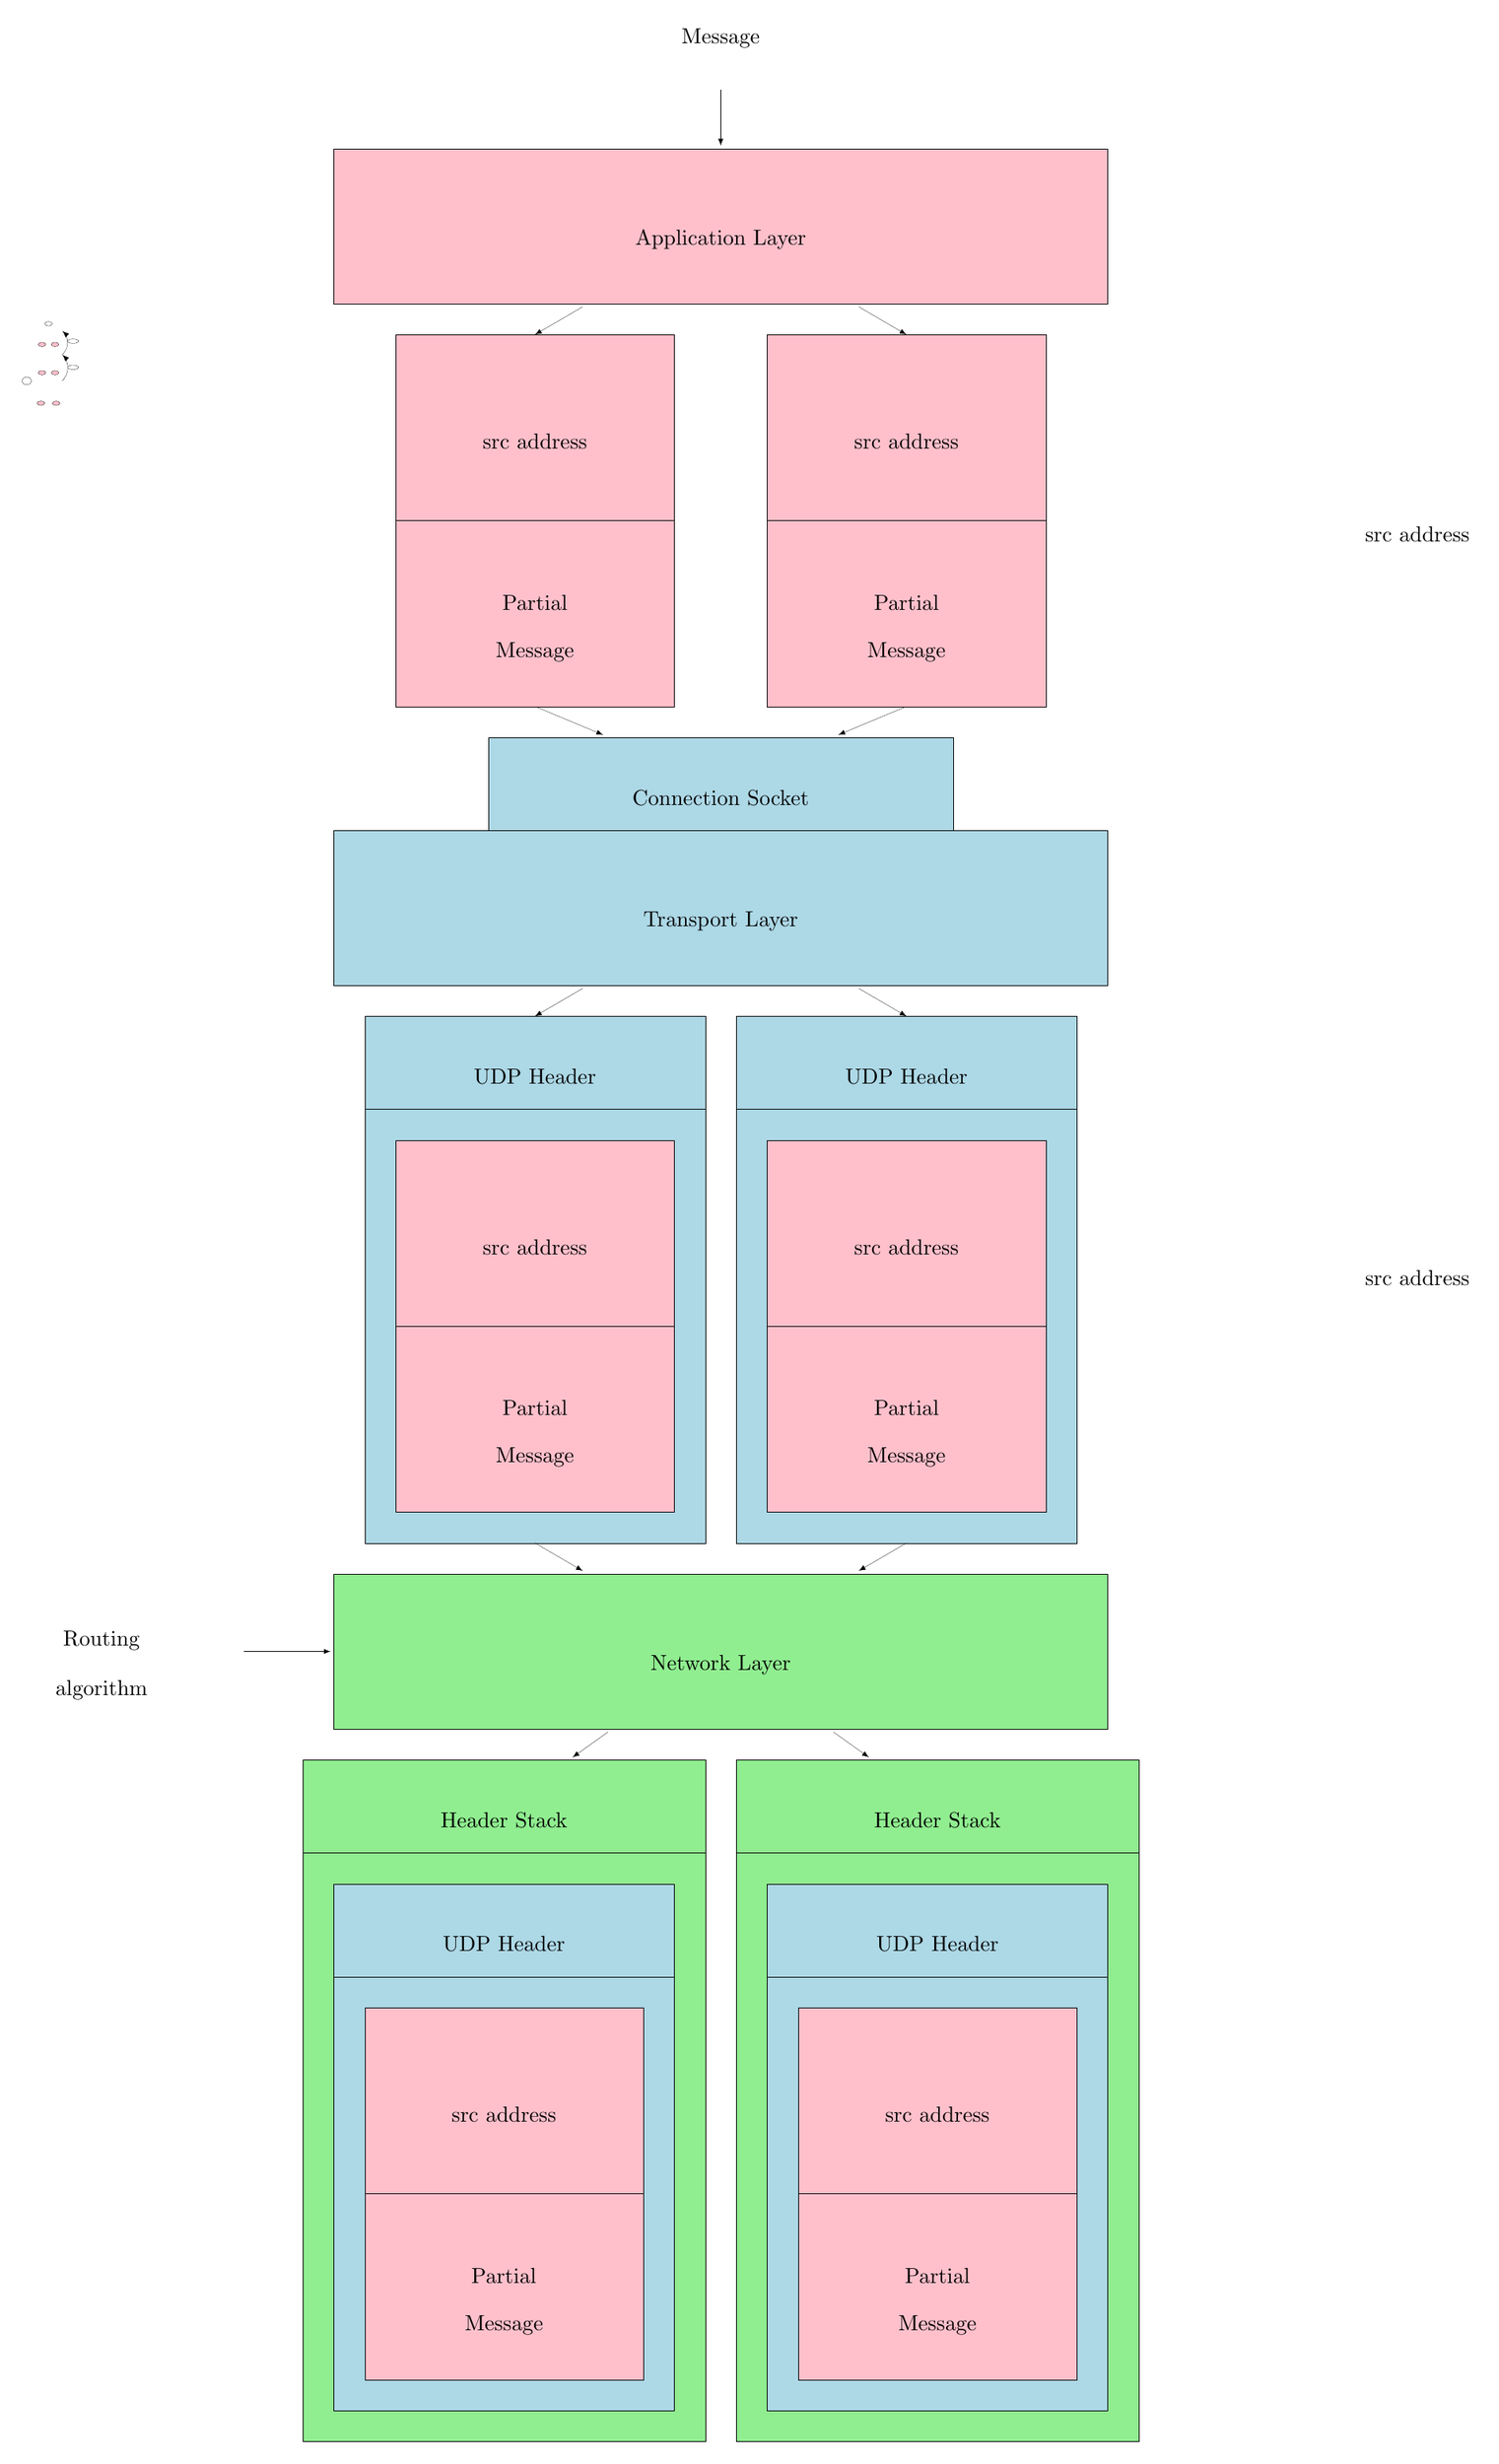
\begin{tikzpicture}
\pgftransformxscale{1.000000}
\pgftransformyscale{-1.000000}
\definecolor{dialinecolor}{rgb}{0.000000, 0.000000, 0.000000}
\pgfsetstrokecolor{dialinecolor}
\definecolor{dialinecolor}{rgb}{1.000000, 1.000000, 1.000000}
\pgfsetfillcolor{dialinecolor}
\pgfsetlinewidth{0.100000\du}
\pgfsetdash{}{0pt}
\pgfsetdash{}{0pt}
\pgfsetmiterjoin
\definecolor{dialinecolor}{rgb}{0.564706, 0.933333, 0.564706}
\pgfsetfillcolor{dialinecolor}
\fill (11.500000\du,24.500000\du)--(11.500000\du,34.000000\du)--(18.000000\du,34.000000\du)--(18.000000\du,24.500000\du)--cycle;
\definecolor{dialinecolor}{rgb}{0.000000, 0.000000, 0.000000}
\pgfsetstrokecolor{dialinecolor}
\draw (11.500000\du,24.500000\du)--(11.500000\du,34.000000\du)--(18.000000\du,34.000000\du)--(18.000000\du,24.500000\du)--cycle;
\pgfsetlinewidth{0.100000\du}
\pgfsetdash{}{0pt}
\pgfsetdash{}{0pt}
\pgfsetmiterjoin
\definecolor{dialinecolor}{rgb}{0.564706, 0.933333, 0.564706}
\pgfsetfillcolor{dialinecolor}
\fill (4.500000\du,24.500000\du)--(4.500000\du,34.000000\du)--(11.000000\du,34.000000\du)--(11.000000\du,24.500000\du)--cycle;
\definecolor{dialinecolor}{rgb}{0.000000, 0.000000, 0.000000}
\pgfsetstrokecolor{dialinecolor}
\draw (4.500000\du,24.500000\du)--(4.500000\du,34.000000\du)--(11.000000\du,34.000000\du)--(11.000000\du,24.500000\du)--cycle;
\pgfsetlinewidth{0.100000\du}
\pgfsetdash{}{0pt}
\pgfsetdash{}{0pt}
\pgfsetmiterjoin
\definecolor{dialinecolor}{rgb}{0.678431, 0.847059, 0.901961}
\pgfsetfillcolor{dialinecolor}
\fill (5.000000\du,8.000000\du)--(5.000000\du,10.500000\du)--(17.500000\du,10.500000\du)--(17.500000\du,8.000000\du)--cycle;
\definecolor{dialinecolor}{rgb}{0.000000, 0.000000, 0.000000}
\pgfsetstrokecolor{dialinecolor}
\draw (5.000000\du,8.000000\du)--(5.000000\du,10.500000\du)--(17.500000\du,10.500000\du)--(17.500000\du,8.000000\du)--cycle;
% setfont left to latex
\definecolor{dialinecolor}{rgb}{0.000000, 0.000000, 0.000000}
\pgfsetstrokecolor{dialinecolor}
\node at (11.250000\du,9.472500\du){Transport Layer};
\pgfsetlinewidth{0.100000\du}
\pgfsetdash{}{0pt}
\pgfsetdash{}{0pt}
\pgfsetmiterjoin
\definecolor{dialinecolor}{rgb}{0.564706, 0.933333, 0.564706}
\pgfsetfillcolor{dialinecolor}
\fill (5.000000\du,20.000000\du)--(5.000000\du,22.500000\du)--(17.500000\du,22.500000\du)--(17.500000\du,20.000000\du)--cycle;
\definecolor{dialinecolor}{rgb}{0.000000, 0.000000, 0.000000}
\pgfsetstrokecolor{dialinecolor}
\draw (5.000000\du,20.000000\du)--(5.000000\du,22.500000\du)--(17.500000\du,22.500000\du)--(17.500000\du,20.000000\du)--cycle;
% setfont left to latex
\definecolor{dialinecolor}{rgb}{0.000000, 0.000000, 0.000000}
\pgfsetstrokecolor{dialinecolor}
\node at (11.250000\du,21.472500\du){Network Layer};
\pgfsetlinewidth{0.100000\du}
\pgfsetdash{}{0pt}
\pgfsetdash{}{0pt}
\pgfsetmiterjoin
\definecolor{dialinecolor}{rgb}{1.000000, 0.752941, 0.796078}
\pgfsetfillcolor{dialinecolor}
\fill (5.000000\du,-3.000000\du)--(5.000000\du,-0.500000\du)--(17.500000\du,-0.500000\du)--(17.500000\du,-3.000000\du)--cycle;
\definecolor{dialinecolor}{rgb}{0.000000, 0.000000, 0.000000}
\pgfsetstrokecolor{dialinecolor}
\draw (5.000000\du,-3.000000\du)--(5.000000\du,-0.500000\du)--(17.500000\du,-0.500000\du)--(17.500000\du,-3.000000\du)--cycle;
% setfont left to latex
\definecolor{dialinecolor}{rgb}{0.000000, 0.000000, 0.000000}
\pgfsetstrokecolor{dialinecolor}
\node at (11.250000\du,-1.527500\du){Application Layer};
\definecolor{dialinecolor}{rgb}{1.000000, 1.000000, 1.000000}
\pgfsetfillcolor{dialinecolor}
\pgfpathellipse{\pgfpoint{11.250000\du}{-5.000000\du}}{\pgfpoint{1.750000\du}{0\du}}{\pgfpoint{0\du}{1.000000\du}}
\pgfusepath{fill}
\pgfsetlinewidth{0.100000\du}
\pgfsetdash{}{0pt}
\pgfsetdash{}{0pt}
\definecolor{dialinecolor}{rgb}{0.000000, 0.000000, 0.000000}
\pgfsetstrokecolor{dialinecolor}
\pgfpathellipse{\pgfpoint{11.250000\du}{-5.000000\du}}{\pgfpoint{1.750000\du}{0\du}}{\pgfpoint{0\du}{1.000000\du}}
\pgfusepath{stroke}
% setfont left to latex
\definecolor{dialinecolor}{rgb}{0.000000, 0.000000, 0.000000}
\pgfsetstrokecolor{dialinecolor}
\node at (11.250000\du,-4.777500\du){Message};
\pgfsetlinewidth{0.100000\du}
\pgfsetdash{}{0pt}
\pgfsetdash{}{0pt}
\pgfsetmiterjoin
\definecolor{dialinecolor}{rgb}{0.678431, 0.847059, 0.901961}
\pgfsetfillcolor{dialinecolor}
\fill (11.500000\du,12.500000\du)--(11.500000\du,19.500000\du)--(17.000000\du,19.500000\du)--(17.000000\du,12.500000\du)--cycle;
\definecolor{dialinecolor}{rgb}{0.000000, 0.000000, 0.000000}
\pgfsetstrokecolor{dialinecolor}
\draw (11.500000\du,12.500000\du)--(11.500000\du,19.500000\du)--(17.000000\du,19.500000\du)--(17.000000\du,12.500000\du)--cycle;
\pgfsetlinewidth{0.100000\du}
\pgfsetdash{}{0pt}
\pgfsetdash{}{0pt}
\pgfsetmiterjoin
\definecolor{dialinecolor}{rgb}{1.000000, 0.752941, 0.796078}
\pgfsetfillcolor{dialinecolor}
\fill (12.000000\du,16.000000\du)--(12.000000\du,19.000000\du)--(16.500000\du,19.000000\du)--(16.500000\du,16.000000\du)--cycle;
\definecolor{dialinecolor}{rgb}{0.000000, 0.000000, 0.000000}
\pgfsetstrokecolor{dialinecolor}
\draw (12.000000\du,16.000000\du)--(12.000000\du,19.000000\du)--(16.500000\du,19.000000\du)--(16.500000\du,16.000000\du)--cycle;
\definecolor{dialinecolor}{rgb}{1.000000, 0.752941, 0.796078}
\pgfsetfillcolor{dialinecolor}
\pgfpathellipse{\pgfpoint{14.250000\du}{17.500000\du}}{\pgfpoint{1.750000\du}{0\du}}{\pgfpoint{0\du}{1.000000\du}}
\pgfusepath{fill}
\pgfsetlinewidth{0.100000\du}
\pgfsetdash{}{0pt}
\pgfsetdash{}{0pt}
\definecolor{dialinecolor}{rgb}{0.000000, 0.000000, 0.000000}
\pgfsetstrokecolor{dialinecolor}
\pgfpathellipse{\pgfpoint{14.250000\du}{17.500000\du}}{\pgfpoint{1.750000\du}{0\du}}{\pgfpoint{0\du}{1.000000\du}}
\pgfusepath{stroke}
\pgfsetlinewidth{0.100000\du}
\pgfsetdash{}{0pt}
\pgfsetdash{}{0pt}
\pgfsetmiterjoin
\definecolor{dialinecolor}{rgb}{1.000000, 0.752941, 0.796078}
\pgfsetfillcolor{dialinecolor}
\fill (12.000000\du,13.000000\du)--(12.000000\du,16.000000\du)--(16.500000\du,16.000000\du)--(16.500000\du,13.000000\du)--cycle;
\definecolor{dialinecolor}{rgb}{0.000000, 0.000000, 0.000000}
\pgfsetstrokecolor{dialinecolor}
\draw (12.000000\du,13.000000\du)--(12.000000\du,16.000000\du)--(16.500000\du,16.000000\du)--(16.500000\du,13.000000\du)--cycle;
% setfont left to latex
\definecolor{dialinecolor}{rgb}{0.000000, 0.000000, 0.000000}
\pgfsetstrokecolor{dialinecolor}
\node at (14.250000\du,14.722500\du){src address};
\pgfsetlinewidth{0.100000\du}
\pgfsetdash{}{0pt}
\pgfsetdash{}{0pt}
\pgfsetmiterjoin
\definecolor{dialinecolor}{rgb}{0.678431, 0.847059, 0.901961}
\pgfsetfillcolor{dialinecolor}
\fill (11.500000\du,11.000000\du)--(11.500000\du,12.500000\du)--(17.000000\du,12.500000\du)--(17.000000\du,11.000000\du)--cycle;
\definecolor{dialinecolor}{rgb}{0.000000, 0.000000, 0.000000}
\pgfsetstrokecolor{dialinecolor}
\draw (11.500000\du,11.000000\du)--(11.500000\du,12.500000\du)--(17.000000\du,12.500000\du)--(17.000000\du,11.000000\du)--cycle;
% setfont left to latex
\definecolor{dialinecolor}{rgb}{0.000000, 0.000000, 0.000000}
\pgfsetstrokecolor{dialinecolor}
\node at (14.250000\du,11.972500\du){UDP Header};
\pgfsetlinewidth{0.100000\du}
\pgfsetdash{}{0pt}
\pgfsetdash{}{0pt}
\pgfsetmiterjoin
\definecolor{dialinecolor}{rgb}{0.678431, 0.847059, 0.901961}
\pgfsetfillcolor{dialinecolor}
\fill (5.500000\du,12.500000\du)--(5.500000\du,19.500000\du)--(11.000000\du,19.500000\du)--(11.000000\du,12.500000\du)--cycle;
\definecolor{dialinecolor}{rgb}{0.000000, 0.000000, 0.000000}
\pgfsetstrokecolor{dialinecolor}
\draw (5.500000\du,12.500000\du)--(5.500000\du,19.500000\du)--(11.000000\du,19.500000\du)--(11.000000\du,12.500000\du)--cycle;
\pgfsetlinewidth{0.100000\du}
\pgfsetdash{}{0pt}
\pgfsetdash{}{0pt}
\pgfsetmiterjoin
\definecolor{dialinecolor}{rgb}{1.000000, 0.752941, 0.796078}
\pgfsetfillcolor{dialinecolor}
\fill (6.000000\du,16.000000\du)--(6.000000\du,19.000000\du)--(10.500000\du,19.000000\du)--(10.500000\du,16.000000\du)--cycle;
\definecolor{dialinecolor}{rgb}{0.000000, 0.000000, 0.000000}
\pgfsetstrokecolor{dialinecolor}
\draw (6.000000\du,16.000000\du)--(6.000000\du,19.000000\du)--(10.500000\du,19.000000\du)--(10.500000\du,16.000000\du)--cycle;
\definecolor{dialinecolor}{rgb}{1.000000, 0.752941, 0.796078}
\pgfsetfillcolor{dialinecolor}
\pgfpathellipse{\pgfpoint{8.250000\du}{17.500000\du}}{\pgfpoint{1.750000\du}{0\du}}{\pgfpoint{0\du}{1.000000\du}}
\pgfusepath{fill}
\pgfsetlinewidth{0.100000\du}
\pgfsetdash{}{0pt}
\pgfsetdash{}{0pt}
\definecolor{dialinecolor}{rgb}{0.000000, 0.000000, 0.000000}
\pgfsetstrokecolor{dialinecolor}
\pgfpathellipse{\pgfpoint{8.250000\du}{17.500000\du}}{\pgfpoint{1.750000\du}{0\du}}{\pgfpoint{0\du}{1.000000\du}}
\pgfusepath{stroke}
\pgfsetlinewidth{0.100000\du}
\pgfsetdash{}{0pt}
\pgfsetdash{}{0pt}
\pgfsetmiterjoin
\definecolor{dialinecolor}{rgb}{1.000000, 0.752941, 0.796078}
\pgfsetfillcolor{dialinecolor}
\fill (6.000000\du,13.000000\du)--(6.000000\du,16.000000\du)--(10.500000\du,16.000000\du)--(10.500000\du,13.000000\du)--cycle;
\definecolor{dialinecolor}{rgb}{0.000000, 0.000000, 0.000000}
\pgfsetstrokecolor{dialinecolor}
\draw (6.000000\du,13.000000\du)--(6.000000\du,16.000000\du)--(10.500000\du,16.000000\du)--(10.500000\du,13.000000\du)--cycle;
% setfont left to latex
\definecolor{dialinecolor}{rgb}{0.000000, 0.000000, 0.000000}
\pgfsetstrokecolor{dialinecolor}
\node at (8.250000\du,14.722500\du){src address};
\pgfsetlinewidth{0.100000\du}
\pgfsetdash{}{0pt}
\pgfsetdash{}{0pt}
\pgfsetmiterjoin
\definecolor{dialinecolor}{rgb}{0.678431, 0.847059, 0.901961}
\pgfsetfillcolor{dialinecolor}
\fill (5.500000\du,11.000000\du)--(5.500000\du,12.500000\du)--(11.000000\du,12.500000\du)--(11.000000\du,11.000000\du)--cycle;
\definecolor{dialinecolor}{rgb}{0.000000, 0.000000, 0.000000}
\pgfsetstrokecolor{dialinecolor}
\draw (5.500000\du,11.000000\du)--(5.500000\du,12.500000\du)--(11.000000\du,12.500000\du)--(11.000000\du,11.000000\du)--cycle;
% setfont left to latex
\definecolor{dialinecolor}{rgb}{0.000000, 0.000000, 0.000000}
\pgfsetstrokecolor{dialinecolor}
\node at (8.250000\du,11.972500\du){UDP Header};
\pgfsetlinewidth{0.100000\du}
\pgfsetdash{}{0pt}
\pgfsetdash{}{0pt}
\pgfsetbuttcap
{
\definecolor{dialinecolor}{rgb}{0.000000, 0.000000, 0.000000}
\pgfsetfillcolor{dialinecolor}
% was here!!!
\pgfsetarrowsend{latex}
\definecolor{dialinecolor}{rgb}{0.000000, 0.000000, 0.000000}
\pgfsetstrokecolor{dialinecolor}
\draw (11.250000\du,-3.951050\du)--(11.250000\du,-3.050079\du);
}
\pgfsetlinewidth{0.100000\du}
\pgfsetdash{}{0pt}
\pgfsetdash{}{0pt}
\pgfsetbuttcap
{
\definecolor{dialinecolor}{rgb}{0.000000, 0.000000, 0.000000}
\pgfsetfillcolor{dialinecolor}
% was here!!!
\pgfsetarrowsend{latex}
\definecolor{dialinecolor}{rgb}{0.000000, 0.000000, 0.000000}
\pgfsetstrokecolor{dialinecolor}
\draw (9.021973\du,-0.450317\du)--(8.250000\du,0.000000\du);
}
\pgfsetlinewidth{0.100000\du}
\pgfsetdash{}{0pt}
\pgfsetdash{}{0pt}
\pgfsetbuttcap
{
\definecolor{dialinecolor}{rgb}{0.000000, 0.000000, 0.000000}
\pgfsetfillcolor{dialinecolor}
% was here!!!
\pgfsetarrowsend{latex}
\definecolor{dialinecolor}{rgb}{0.000000, 0.000000, 0.000000}
\pgfsetstrokecolor{dialinecolor}
\draw (13.478027\du,-0.450317\du)--(14.250000\du,0.000000\du);
}
\pgfsetlinewidth{0.100000\du}
\pgfsetdash{}{0pt}
\pgfsetdash{}{0pt}
\pgfsetbuttcap
{
\definecolor{dialinecolor}{rgb}{0.000000, 0.000000, 0.000000}
\pgfsetfillcolor{dialinecolor}
% was here!!!
\pgfsetarrowsend{latex}
\definecolor{dialinecolor}{rgb}{0.000000, 0.000000, 0.000000}
\pgfsetstrokecolor{dialinecolor}
\draw (9.021973\du,10.549683\du)--(8.250000\du,11.000000\du);
}
\pgfsetlinewidth{0.100000\du}
\pgfsetdash{}{0pt}
\pgfsetdash{}{0pt}
\pgfsetbuttcap
{
\definecolor{dialinecolor}{rgb}{0.000000, 0.000000, 0.000000}
\pgfsetfillcolor{dialinecolor}
% was here!!!
\pgfsetarrowsend{latex}
\definecolor{dialinecolor}{rgb}{0.000000, 0.000000, 0.000000}
\pgfsetstrokecolor{dialinecolor}
\draw (13.478027\du,10.549683\du)--(14.250000\du,11.000000\du);
}
\definecolor{dialinecolor}{rgb}{1.000000, 1.000000, 1.000000}
\pgfsetfillcolor{dialinecolor}
\pgfpathellipse{\pgfpoint{1.250000\du}{21.250000\du}}{\pgfpoint{2.250000\du}{0\du}}{\pgfpoint{0\du}{1.750000\du}}
\pgfusepath{fill}
\pgfsetlinewidth{0.100000\du}
\pgfsetdash{}{0pt}
\pgfsetdash{}{0pt}
\definecolor{dialinecolor}{rgb}{0.000000, 0.000000, 0.000000}
\pgfsetstrokecolor{dialinecolor}
\pgfpathellipse{\pgfpoint{1.250000\du}{21.250000\du}}{\pgfpoint{2.250000\du}{0\du}}{\pgfpoint{0\du}{1.750000\du}}
\pgfusepath{stroke}
% setfont left to latex
\definecolor{dialinecolor}{rgb}{0.000000, 0.000000, 0.000000}
\pgfsetstrokecolor{dialinecolor}
\node at (1.250000\du,21.072500\du){Routing};
% setfont left to latex
\definecolor{dialinecolor}{rgb}{0.000000, 0.000000, 0.000000}
\pgfsetstrokecolor{dialinecolor}
\node at (1.250000\du,21.872500\du){algorithm};
\pgfsetlinewidth{0.100000\du}
\pgfsetdash{}{0pt}
\pgfsetdash{}{0pt}
\pgfsetbuttcap
{
\definecolor{dialinecolor}{rgb}{0.000000, 0.000000, 0.000000}
\pgfsetfillcolor{dialinecolor}
% was here!!!
\pgfsetarrowsend{latex}
\definecolor{dialinecolor}{rgb}{0.000000, 0.000000, 0.000000}
\pgfsetstrokecolor{dialinecolor}
\draw (3.550110\du,21.250000\du)--(4.950562\du,21.250000\du);
}
\pgfsetlinewidth{0.100000\du}
\pgfsetdash{}{0pt}
\pgfsetdash{}{0pt}
\pgfsetbuttcap
{
\definecolor{dialinecolor}{rgb}{0.000000, 0.000000, 0.000000}
\pgfsetfillcolor{dialinecolor}
% was here!!!
\pgfsetarrowsend{latex}
\definecolor{dialinecolor}{rgb}{0.000000, 0.000000, 0.000000}
\pgfsetstrokecolor{dialinecolor}
\draw (8.250000\du,19.500000\du)--(9.021973\du,19.950317\du);
}
\pgfsetlinewidth{0.100000\du}
\pgfsetdash{}{0pt}
\pgfsetdash{}{0pt}
\pgfsetbuttcap
{
\definecolor{dialinecolor}{rgb}{0.000000, 0.000000, 0.000000}
\pgfsetfillcolor{dialinecolor}
% was here!!!
\pgfsetarrowsend{latex}
\definecolor{dialinecolor}{rgb}{0.000000, 0.000000, 0.000000}
\pgfsetstrokecolor{dialinecolor}
\draw (14.250000\du,19.500000\du)--(13.478027\du,19.950317\du);
}
\pgfsetlinewidth{0.100000\du}
\pgfsetdash{}{0pt}
\pgfsetdash{}{0pt}
\pgfsetbuttcap
{
\definecolor{dialinecolor}{rgb}{0.000000, 0.000000, 0.000000}
\pgfsetfillcolor{dialinecolor}
% was here!!!
\pgfsetarrowsend{latex}
\definecolor{dialinecolor}{rgb}{0.000000, 0.000000, 0.000000}
\pgfsetstrokecolor{dialinecolor}
\pgfpathmoveto{\pgfpoint{17.499448\du}{21.250548\du}}
\pgfpatharc{46}{-45}{8.450000\du and 8.450000\du}
\pgfusepath{stroke}
}
\definecolor{dialinecolor}{rgb}{1.000000, 1.000000, 1.000000}
\pgfsetfillcolor{dialinecolor}
\pgfpathellipse{\pgfpoint{22.500000\du}{15.000000\du}}{\pgfpoint{2.500000\du}{0\du}}{\pgfpoint{0\du}{1.000000\du}}
\pgfusepath{fill}
\pgfsetlinewidth{0.100000\du}
\pgfsetdash{}{0pt}
\pgfsetdash{}{0pt}
\definecolor{dialinecolor}{rgb}{0.000000, 0.000000, 0.000000}
\pgfsetstrokecolor{dialinecolor}
\pgfpathellipse{\pgfpoint{22.500000\du}{15.000000\du}}{\pgfpoint{2.500000\du}{0\du}}{\pgfpoint{0\du}{1.000000\du}}
\pgfusepath{stroke}
% setfont left to latex
\definecolor{dialinecolor}{rgb}{0.000000, 0.000000, 0.000000}
\pgfsetstrokecolor{dialinecolor}
\node at (22.500000\du,15.222500\du){src address};
\pgfsetlinewidth{0.100000\du}
\pgfsetdash{}{0pt}
\pgfsetdash{}{0pt}
\pgfsetmiterjoin
\definecolor{dialinecolor}{rgb}{0.678431, 0.847059, 0.901961}
\pgfsetfillcolor{dialinecolor}
\fill (5.000000\du,26.500000\du)--(5.000000\du,33.500000\du)--(10.500000\du,33.500000\du)--(10.500000\du,26.500000\du)--cycle;
\definecolor{dialinecolor}{rgb}{0.000000, 0.000000, 0.000000}
\pgfsetstrokecolor{dialinecolor}
\draw (5.000000\du,26.500000\du)--(5.000000\du,33.500000\du)--(10.500000\du,33.500000\du)--(10.500000\du,26.500000\du)--cycle;
\pgfsetlinewidth{0.100000\du}
\pgfsetdash{}{0pt}
\pgfsetdash{}{0pt}
\pgfsetmiterjoin
\definecolor{dialinecolor}{rgb}{1.000000, 0.752941, 0.796078}
\pgfsetfillcolor{dialinecolor}
\fill (5.500000\du,30.000000\du)--(5.500000\du,33.000000\du)--(10.000000\du,33.000000\du)--(10.000000\du,30.000000\du)--cycle;
\definecolor{dialinecolor}{rgb}{0.000000, 0.000000, 0.000000}
\pgfsetstrokecolor{dialinecolor}
\draw (5.500000\du,30.000000\du)--(5.500000\du,33.000000\du)--(10.000000\du,33.000000\du)--(10.000000\du,30.000000\du)--cycle;
\definecolor{dialinecolor}{rgb}{1.000000, 0.752941, 0.796078}
\pgfsetfillcolor{dialinecolor}
\pgfpathellipse{\pgfpoint{7.750000\du}{31.500000\du}}{\pgfpoint{1.750000\du}{0\du}}{\pgfpoint{0\du}{1.000000\du}}
\pgfusepath{fill}
\pgfsetlinewidth{0.100000\du}
\pgfsetdash{}{0pt}
\pgfsetdash{}{0pt}
\definecolor{dialinecolor}{rgb}{0.000000, 0.000000, 0.000000}
\pgfsetstrokecolor{dialinecolor}
\pgfpathellipse{\pgfpoint{7.750000\du}{31.500000\du}}{\pgfpoint{1.750000\du}{0\du}}{\pgfpoint{0\du}{1.000000\du}}
\pgfusepath{stroke}
\pgfsetlinewidth{0.100000\du}
\pgfsetdash{}{0pt}
\pgfsetdash{}{0pt}
\pgfsetmiterjoin
\definecolor{dialinecolor}{rgb}{1.000000, 0.752941, 0.796078}
\pgfsetfillcolor{dialinecolor}
\fill (5.500000\du,27.000000\du)--(5.500000\du,30.000000\du)--(10.000000\du,30.000000\du)--(10.000000\du,27.000000\du)--cycle;
\definecolor{dialinecolor}{rgb}{0.000000, 0.000000, 0.000000}
\pgfsetstrokecolor{dialinecolor}
\draw (5.500000\du,27.000000\du)--(5.500000\du,30.000000\du)--(10.000000\du,30.000000\du)--(10.000000\du,27.000000\du)--cycle;
% setfont left to latex
\definecolor{dialinecolor}{rgb}{0.000000, 0.000000, 0.000000}
\pgfsetstrokecolor{dialinecolor}
\node at (7.750000\du,28.722500\du){src address};
\pgfsetlinewidth{0.100000\du}
\pgfsetdash{}{0pt}
\pgfsetdash{}{0pt}
\pgfsetmiterjoin
\definecolor{dialinecolor}{rgb}{0.678431, 0.847059, 0.901961}
\pgfsetfillcolor{dialinecolor}
\fill (5.000000\du,25.000000\du)--(5.000000\du,26.500000\du)--(10.500000\du,26.500000\du)--(10.500000\du,25.000000\du)--cycle;
\definecolor{dialinecolor}{rgb}{0.000000, 0.000000, 0.000000}
\pgfsetstrokecolor{dialinecolor}
\draw (5.000000\du,25.000000\du)--(5.000000\du,26.500000\du)--(10.500000\du,26.500000\du)--(10.500000\du,25.000000\du)--cycle;
% setfont left to latex
\definecolor{dialinecolor}{rgb}{0.000000, 0.000000, 0.000000}
\pgfsetstrokecolor{dialinecolor}
\node at (7.750000\du,25.972500\du){UDP Header};
\pgfsetlinewidth{0.100000\du}
\pgfsetdash{}{0pt}
\pgfsetdash{}{0pt}
\pgfsetmiterjoin
\definecolor{dialinecolor}{rgb}{0.678431, 0.847059, 0.901961}
\pgfsetfillcolor{dialinecolor}
\fill (12.000000\du,26.500000\du)--(12.000000\du,33.500000\du)--(17.500000\du,33.500000\du)--(17.500000\du,26.500000\du)--cycle;
\definecolor{dialinecolor}{rgb}{0.000000, 0.000000, 0.000000}
\pgfsetstrokecolor{dialinecolor}
\draw (12.000000\du,26.500000\du)--(12.000000\du,33.500000\du)--(17.500000\du,33.500000\du)--(17.500000\du,26.500000\du)--cycle;
\pgfsetlinewidth{0.100000\du}
\pgfsetdash{}{0pt}
\pgfsetdash{}{0pt}
\pgfsetmiterjoin
\definecolor{dialinecolor}{rgb}{1.000000, 0.752941, 0.796078}
\pgfsetfillcolor{dialinecolor}
\fill (12.500000\du,30.000000\du)--(12.500000\du,33.000000\du)--(17.000000\du,33.000000\du)--(17.000000\du,30.000000\du)--cycle;
\definecolor{dialinecolor}{rgb}{0.000000, 0.000000, 0.000000}
\pgfsetstrokecolor{dialinecolor}
\draw (12.500000\du,30.000000\du)--(12.500000\du,33.000000\du)--(17.000000\du,33.000000\du)--(17.000000\du,30.000000\du)--cycle;
\definecolor{dialinecolor}{rgb}{1.000000, 0.752941, 0.796078}
\pgfsetfillcolor{dialinecolor}
\pgfpathellipse{\pgfpoint{14.750000\du}{31.500000\du}}{\pgfpoint{1.750000\du}{0\du}}{\pgfpoint{0\du}{1.000000\du}}
\pgfusepath{fill}
\pgfsetlinewidth{0.100000\du}
\pgfsetdash{}{0pt}
\pgfsetdash{}{0pt}
\definecolor{dialinecolor}{rgb}{0.000000, 0.000000, 0.000000}
\pgfsetstrokecolor{dialinecolor}
\pgfpathellipse{\pgfpoint{14.750000\du}{31.500000\du}}{\pgfpoint{1.750000\du}{0\du}}{\pgfpoint{0\du}{1.000000\du}}
\pgfusepath{stroke}
\pgfsetlinewidth{0.100000\du}
\pgfsetdash{}{0pt}
\pgfsetdash{}{0pt}
\pgfsetmiterjoin
\definecolor{dialinecolor}{rgb}{1.000000, 0.752941, 0.796078}
\pgfsetfillcolor{dialinecolor}
\fill (12.500000\du,27.000000\du)--(12.500000\du,30.000000\du)--(17.000000\du,30.000000\du)--(17.000000\du,27.000000\du)--cycle;
\definecolor{dialinecolor}{rgb}{0.000000, 0.000000, 0.000000}
\pgfsetstrokecolor{dialinecolor}
\draw (12.500000\du,27.000000\du)--(12.500000\du,30.000000\du)--(17.000000\du,30.000000\du)--(17.000000\du,27.000000\du)--cycle;
% setfont left to latex
\definecolor{dialinecolor}{rgb}{0.000000, 0.000000, 0.000000}
\pgfsetstrokecolor{dialinecolor}
\node at (14.750000\du,28.722500\du){src address};
\pgfsetlinewidth{0.100000\du}
\pgfsetdash{}{0pt}
\pgfsetdash{}{0pt}
\pgfsetmiterjoin
\definecolor{dialinecolor}{rgb}{0.678431, 0.847059, 0.901961}
\pgfsetfillcolor{dialinecolor}
\fill (12.000000\du,25.000000\du)--(12.000000\du,26.500000\du)--(17.500000\du,26.500000\du)--(17.500000\du,25.000000\du)--cycle;
\definecolor{dialinecolor}{rgb}{0.000000, 0.000000, 0.000000}
\pgfsetstrokecolor{dialinecolor}
\draw (12.000000\du,25.000000\du)--(12.000000\du,26.500000\du)--(17.500000\du,26.500000\du)--(17.500000\du,25.000000\du)--cycle;
% setfont left to latex
\definecolor{dialinecolor}{rgb}{0.000000, 0.000000, 0.000000}
\pgfsetstrokecolor{dialinecolor}
\node at (14.750000\du,25.972500\du){UDP Header};
\pgfsetlinewidth{0.100000\du}
\pgfsetdash{}{0pt}
\pgfsetdash{}{0pt}
\pgfsetmiterjoin
\definecolor{dialinecolor}{rgb}{0.564706, 0.933333, 0.564706}
\pgfsetfillcolor{dialinecolor}
\fill (4.500000\du,23.000000\du)--(4.500000\du,24.500000\du)--(11.000000\du,24.500000\du)--(11.000000\du,23.000000\du)--cycle;
\definecolor{dialinecolor}{rgb}{0.000000, 0.000000, 0.000000}
\pgfsetstrokecolor{dialinecolor}
\draw (4.500000\du,23.000000\du)--(4.500000\du,24.500000\du)--(11.000000\du,24.500000\du)--(11.000000\du,23.000000\du)--cycle;
% setfont left to latex
\definecolor{dialinecolor}{rgb}{0.000000, 0.000000, 0.000000}
\pgfsetstrokecolor{dialinecolor}
\node at (7.750000\du,23.972500\du){Header Stack};
\pgfsetlinewidth{0.100000\du}
\pgfsetdash{}{0pt}
\pgfsetdash{}{0pt}
\pgfsetmiterjoin
\definecolor{dialinecolor}{rgb}{0.564706, 0.933333, 0.564706}
\pgfsetfillcolor{dialinecolor}
\fill (11.500000\du,23.000000\du)--(11.500000\du,24.500000\du)--(18.000000\du,24.500000\du)--(18.000000\du,23.000000\du)--cycle;
\definecolor{dialinecolor}{rgb}{0.000000, 0.000000, 0.000000}
\pgfsetstrokecolor{dialinecolor}
\draw (11.500000\du,23.000000\du)--(11.500000\du,24.500000\du)--(18.000000\du,24.500000\du)--(18.000000\du,23.000000\du)--cycle;
% setfont left to latex
\definecolor{dialinecolor}{rgb}{0.000000, 0.000000, 0.000000}
\pgfsetstrokecolor{dialinecolor}
\node at (14.750000\du,23.972500\du){Header Stack};
\pgfsetlinewidth{0.100000\du}
\pgfsetdash{}{0pt}
\pgfsetdash{}{0pt}
\pgfsetbuttcap
{
\definecolor{dialinecolor}{rgb}{0.000000, 0.000000, 0.000000}
\pgfsetfillcolor{dialinecolor}
% was here!!!
\pgfsetarrowsend{latex}
\definecolor{dialinecolor}{rgb}{0.000000, 0.000000, 0.000000}
\pgfsetstrokecolor{dialinecolor}
\draw (8.250000\du,6.000000\du)--(9.351562\du,6.458984\du);
}
\pgfsetlinewidth{0.100000\du}
\pgfsetdash{}{0pt}
\pgfsetdash{}{0pt}
\pgfsetbuttcap
{
\definecolor{dialinecolor}{rgb}{0.000000, 0.000000, 0.000000}
\pgfsetfillcolor{dialinecolor}
% was here!!!
\pgfsetarrowsend{latex}
\definecolor{dialinecolor}{rgb}{0.000000, 0.000000, 0.000000}
\pgfsetstrokecolor{dialinecolor}
\draw (14.250000\du,6.000000\du)--(13.148438\du,6.458984\du);
}
\pgfsetlinewidth{0.100000\du}
\pgfsetdash{}{0pt}
\pgfsetdash{}{0pt}
\pgfsetbuttcap
{
\definecolor{dialinecolor}{rgb}{0.000000, 0.000000, 0.000000}
\pgfsetfillcolor{dialinecolor}
% was here!!!
\pgfsetarrowsend{latex}
\definecolor{dialinecolor}{rgb}{0.000000, 0.000000, 0.000000}
\pgfsetstrokecolor{dialinecolor}
\draw (9.430786\du,22.549438\du)--(8.857422\du,22.958984\du);
}
\pgfsetlinewidth{0.100000\du}
\pgfsetdash{}{0pt}
\pgfsetdash{}{0pt}
\pgfsetbuttcap
{
\definecolor{dialinecolor}{rgb}{0.000000, 0.000000, 0.000000}
\pgfsetfillcolor{dialinecolor}
% was here!!!
\pgfsetarrowsend{latex}
\definecolor{dialinecolor}{rgb}{0.000000, 0.000000, 0.000000}
\pgfsetstrokecolor{dialinecolor}
\draw (13.069214\du,22.549438\du)--(13.642578\du,22.958984\du);
}
\pgfsetlinewidth{0.100000\du}
\pgfsetdash{}{0pt}
\pgfsetdash{}{0pt}
\pgfsetmiterjoin
\definecolor{dialinecolor}{rgb}{1.000000, 0.752941, 0.796078}
\pgfsetfillcolor{dialinecolor}
\fill (12.000000\du,3.000000\du)--(12.000000\du,6.000000\du)--(16.500000\du,6.000000\du)--(16.500000\du,3.000000\du)--cycle;
\definecolor{dialinecolor}{rgb}{0.000000, 0.000000, 0.000000}
\pgfsetstrokecolor{dialinecolor}
\draw (12.000000\du,3.000000\du)--(12.000000\du,6.000000\du)--(16.500000\du,6.000000\du)--(16.500000\du,3.000000\du)--cycle;
\definecolor{dialinecolor}{rgb}{1.000000, 0.752941, 0.796078}
\pgfsetfillcolor{dialinecolor}
\pgfpathellipse{\pgfpoint{14.250000\du}{4.500000\du}}{\pgfpoint{1.750000\du}{0\du}}{\pgfpoint{0\du}{1.000000\du}}
\pgfusepath{fill}
\pgfsetlinewidth{0.100000\du}
\pgfsetdash{}{0pt}
\pgfsetdash{}{0pt}
\definecolor{dialinecolor}{rgb}{0.000000, 0.000000, 0.000000}
\pgfsetstrokecolor{dialinecolor}
\pgfpathellipse{\pgfpoint{14.250000\du}{4.500000\du}}{\pgfpoint{1.750000\du}{0\du}}{\pgfpoint{0\du}{1.000000\du}}
\pgfusepath{stroke}
\pgfsetlinewidth{0.100000\du}
\pgfsetdash{}{0pt}
\pgfsetdash{}{0pt}
\pgfsetmiterjoin
\definecolor{dialinecolor}{rgb}{1.000000, 0.752941, 0.796078}
\pgfsetfillcolor{dialinecolor}
\fill (12.000000\du,0.000000\du)--(12.000000\du,3.000000\du)--(16.500000\du,3.000000\du)--(16.500000\du,0.000000\du)--cycle;
\definecolor{dialinecolor}{rgb}{0.000000, 0.000000, 0.000000}
\pgfsetstrokecolor{dialinecolor}
\draw (12.000000\du,0.000000\du)--(12.000000\du,3.000000\du)--(16.500000\du,3.000000\du)--(16.500000\du,0.000000\du)--cycle;
% setfont left to latex
\definecolor{dialinecolor}{rgb}{0.000000, 0.000000, 0.000000}
\pgfsetstrokecolor{dialinecolor}
\node at (14.250000\du,1.722500\du){src address};
% setfont left to latex
\definecolor{dialinecolor}{rgb}{0.000000, 0.000000, 0.000000}
\pgfsetstrokecolor{dialinecolor}
\node at (14.250000\du,4.322500\du){Partial};
% setfont left to latex
\definecolor{dialinecolor}{rgb}{0.000000, 0.000000, 0.000000}
\pgfsetstrokecolor{dialinecolor}
\node at (14.250000\du,5.122500\du){Message};
\pgfsetlinewidth{0.100000\du}
\pgfsetdash{}{0pt}
\pgfsetdash{}{0pt}
\pgfsetmiterjoin
\definecolor{dialinecolor}{rgb}{1.000000, 0.752941, 0.796078}
\pgfsetfillcolor{dialinecolor}
\fill (6.000000\du,3.000000\du)--(6.000000\du,6.000000\du)--(10.500000\du,6.000000\du)--(10.500000\du,3.000000\du)--cycle;
\definecolor{dialinecolor}{rgb}{0.000000, 0.000000, 0.000000}
\pgfsetstrokecolor{dialinecolor}
\draw (6.000000\du,3.000000\du)--(6.000000\du,6.000000\du)--(10.500000\du,6.000000\du)--(10.500000\du,3.000000\du)--cycle;
\definecolor{dialinecolor}{rgb}{1.000000, 0.752941, 0.796078}
\pgfsetfillcolor{dialinecolor}
\pgfpathellipse{\pgfpoint{8.250000\du}{4.500000\du}}{\pgfpoint{1.750000\du}{0\du}}{\pgfpoint{0\du}{1.000000\du}}
\pgfusepath{fill}
\pgfsetlinewidth{0.100000\du}
\pgfsetdash{}{0pt}
\pgfsetdash{}{0pt}
\definecolor{dialinecolor}{rgb}{0.000000, 0.000000, 0.000000}
\pgfsetstrokecolor{dialinecolor}
\pgfpathellipse{\pgfpoint{8.250000\du}{4.500000\du}}{\pgfpoint{1.750000\du}{0\du}}{\pgfpoint{0\du}{1.000000\du}}
\pgfusepath{stroke}
\pgfsetlinewidth{0.100000\du}
\pgfsetdash{}{0pt}
\pgfsetdash{}{0pt}
\pgfsetmiterjoin
\definecolor{dialinecolor}{rgb}{1.000000, 0.752941, 0.796078}
\pgfsetfillcolor{dialinecolor}
\fill (6.000000\du,0.000000\du)--(6.000000\du,3.000000\du)--(10.500000\du,3.000000\du)--(10.500000\du,0.000000\du)--cycle;
\definecolor{dialinecolor}{rgb}{0.000000, 0.000000, 0.000000}
\pgfsetstrokecolor{dialinecolor}
\draw (6.000000\du,0.000000\du)--(6.000000\du,3.000000\du)--(10.500000\du,3.000000\du)--(10.500000\du,0.000000\du)--cycle;
% setfont left to latex
\definecolor{dialinecolor}{rgb}{0.000000, 0.000000, 0.000000}
\pgfsetstrokecolor{dialinecolor}
\node at (8.250000\du,1.722500\du){src address};
% setfont left to latex
\definecolor{dialinecolor}{rgb}{0.000000, 0.000000, 0.000000}
\pgfsetstrokecolor{dialinecolor}
\node at (8.250000\du,4.322500\du){Partial};
% setfont left to latex
\definecolor{dialinecolor}{rgb}{0.000000, 0.000000, 0.000000}
\pgfsetstrokecolor{dialinecolor}
\node at (8.250000\du,5.122500\du){Message};
% setfont left to latex
\definecolor{dialinecolor}{rgb}{0.000000, 0.000000, 0.000000}
\pgfsetstrokecolor{dialinecolor}
\node at (8.250000\du,17.322500\du){Partial};
% setfont left to latex
\definecolor{dialinecolor}{rgb}{0.000000, 0.000000, 0.000000}
\pgfsetstrokecolor{dialinecolor}
\node at (8.250000\du,18.122500\du){Message};
% setfont left to latex
\definecolor{dialinecolor}{rgb}{0.000000, 0.000000, 0.000000}
\pgfsetstrokecolor{dialinecolor}
\node at (14.250000\du,17.322500\du){Partial};
% setfont left to latex
\definecolor{dialinecolor}{rgb}{0.000000, 0.000000, 0.000000}
\pgfsetstrokecolor{dialinecolor}
\node at (14.250000\du,18.122500\du){Message};
% setfont left to latex
\definecolor{dialinecolor}{rgb}{0.000000, 0.000000, 0.000000}
\pgfsetstrokecolor{dialinecolor}
\node at (14.750000\du,31.322500\du){Partial};
% setfont left to latex
\definecolor{dialinecolor}{rgb}{0.000000, 0.000000, 0.000000}
\pgfsetstrokecolor{dialinecolor}
\node at (14.750000\du,32.122500\du){Message};
% setfont left to latex
\definecolor{dialinecolor}{rgb}{0.000000, 0.000000, 0.000000}
\pgfsetstrokecolor{dialinecolor}
\node at (7.750000\du,31.322500\du){Partial};
% setfont left to latex
\definecolor{dialinecolor}{rgb}{0.000000, 0.000000, 0.000000}
\pgfsetstrokecolor{dialinecolor}
\node at (7.750000\du,32.122500\du){Message};
\pgfsetlinewidth{0.100000\du}
\pgfsetdash{}{0pt}
\pgfsetdash{}{0pt}
\pgfsetbuttcap
{
\definecolor{dialinecolor}{rgb}{0.000000, 0.000000, 0.000000}
\pgfsetfillcolor{dialinecolor}
% was here!!!
\pgfsetarrowsend{latex}
\definecolor{dialinecolor}{rgb}{0.000000, 0.000000, 0.000000}
\pgfsetstrokecolor{dialinecolor}
\pgfpathmoveto{\pgfpoint{17.499499\du}{9.250437\du}}
\pgfpatharc{49}{-48}{7.300000\du and 7.300000\du}
\pgfusepath{stroke}
}
\definecolor{dialinecolor}{rgb}{1.000000, 1.000000, 1.000000}
\pgfsetfillcolor{dialinecolor}
\pgfpathellipse{\pgfpoint{22.500000\du}{3.000000\du}}{\pgfpoint{2.500000\du}{0\du}}{\pgfpoint{0\du}{1.000000\du}}
\pgfusepath{fill}
\pgfsetlinewidth{0.100000\du}
\pgfsetdash{}{0pt}
\pgfsetdash{}{0pt}
\definecolor{dialinecolor}{rgb}{0.000000, 0.000000, 0.000000}
\pgfsetstrokecolor{dialinecolor}
\pgfpathellipse{\pgfpoint{22.500000\du}{3.000000\du}}{\pgfpoint{2.500000\du}{0\du}}{\pgfpoint{0\du}{1.000000\du}}
\pgfusepath{stroke}
% setfont left to latex
\definecolor{dialinecolor}{rgb}{0.000000, 0.000000, 0.000000}
\pgfsetstrokecolor{dialinecolor}
\node at (22.500000\du,3.222500\du){src address};
\pgfsetlinewidth{0.100000\du}
\pgfsetdash{}{0pt}
\pgfsetdash{}{0pt}
\pgfsetmiterjoin
\definecolor{dialinecolor}{rgb}{0.678431, 0.847059, 0.901961}
\pgfsetfillcolor{dialinecolor}
\fill (7.500000\du,6.500000\du)--(7.500000\du,8.000000\du)--(15.000000\du,8.000000\du)--(15.000000\du,6.500000\du)--cycle;
\definecolor{dialinecolor}{rgb}{0.000000, 0.000000, 0.000000}
\pgfsetstrokecolor{dialinecolor}
\draw (7.500000\du,6.500000\du)--(7.500000\du,8.000000\du)--(15.000000\du,8.000000\du)--(15.000000\du,6.500000\du)--cycle;
% setfont left to latex
\definecolor{dialinecolor}{rgb}{0.000000, 0.000000, 0.000000}
\pgfsetstrokecolor{dialinecolor}
\node at (11.250000\du,7.472500\du){Connection Socket};
\end{tikzpicture}

  \endgroup
  \caption{Pattern of modified OSI, sender side.}
  \label{fig:OSImodified}
\end{figure}

\section{Complete receiver pattern}
A complete picture is printed in page \pageref{fig:OSImodified2}
\subsection{Network Layer :}
\paragraph{When receiving a packet :}
If the header stack contains only one element, the packet is for Bob. Thus decapsulate the packet, and pass it to the transport layer. Otherwise, remove the top header, and forward the packet. 
\subsection{Transport Layer :}
It is just a UDP protocol.
\subsection{Application Layer :}
\paragraph{On default port :}
When receiving a set of messages on the default port, Bob should xor-compose them. If it makes sense (i.e.: if it is a valid handshake), Bob should open a new socket, dedicated to the connection with Alice. Then he acknoledge from that socket. 
\paragraph{On a dedicated port :}
Then, Bob should wait and compose until the message make sense. Indeed, since submessages goes through different paths, the RTT might be different. If the validity time is over, Bob drops the concerned submessage.
\begin{figure}
  \centering
  \begingroup
  \tikzset{every picture/.style={scale=0.8}}
  % Graphic for TeX using PGF
% Title: /home/martin/Documents/EPFL/Semestre III/CompNet/Essay/OSI_establishing.dia
% Creator: Dia v0.97.2
% CreationDate: Sun Dec 22 20:55:34 2013
% For: martin
% \usepackage{tikz}
% The following commands are not supported in PSTricks at present
% We define them conditionally, so when they are implemented,
% this pgf file will use them.
\ifx\du\undefined
  \newlength{\du}
\fi
\setlength{\du}{15\unitlength}
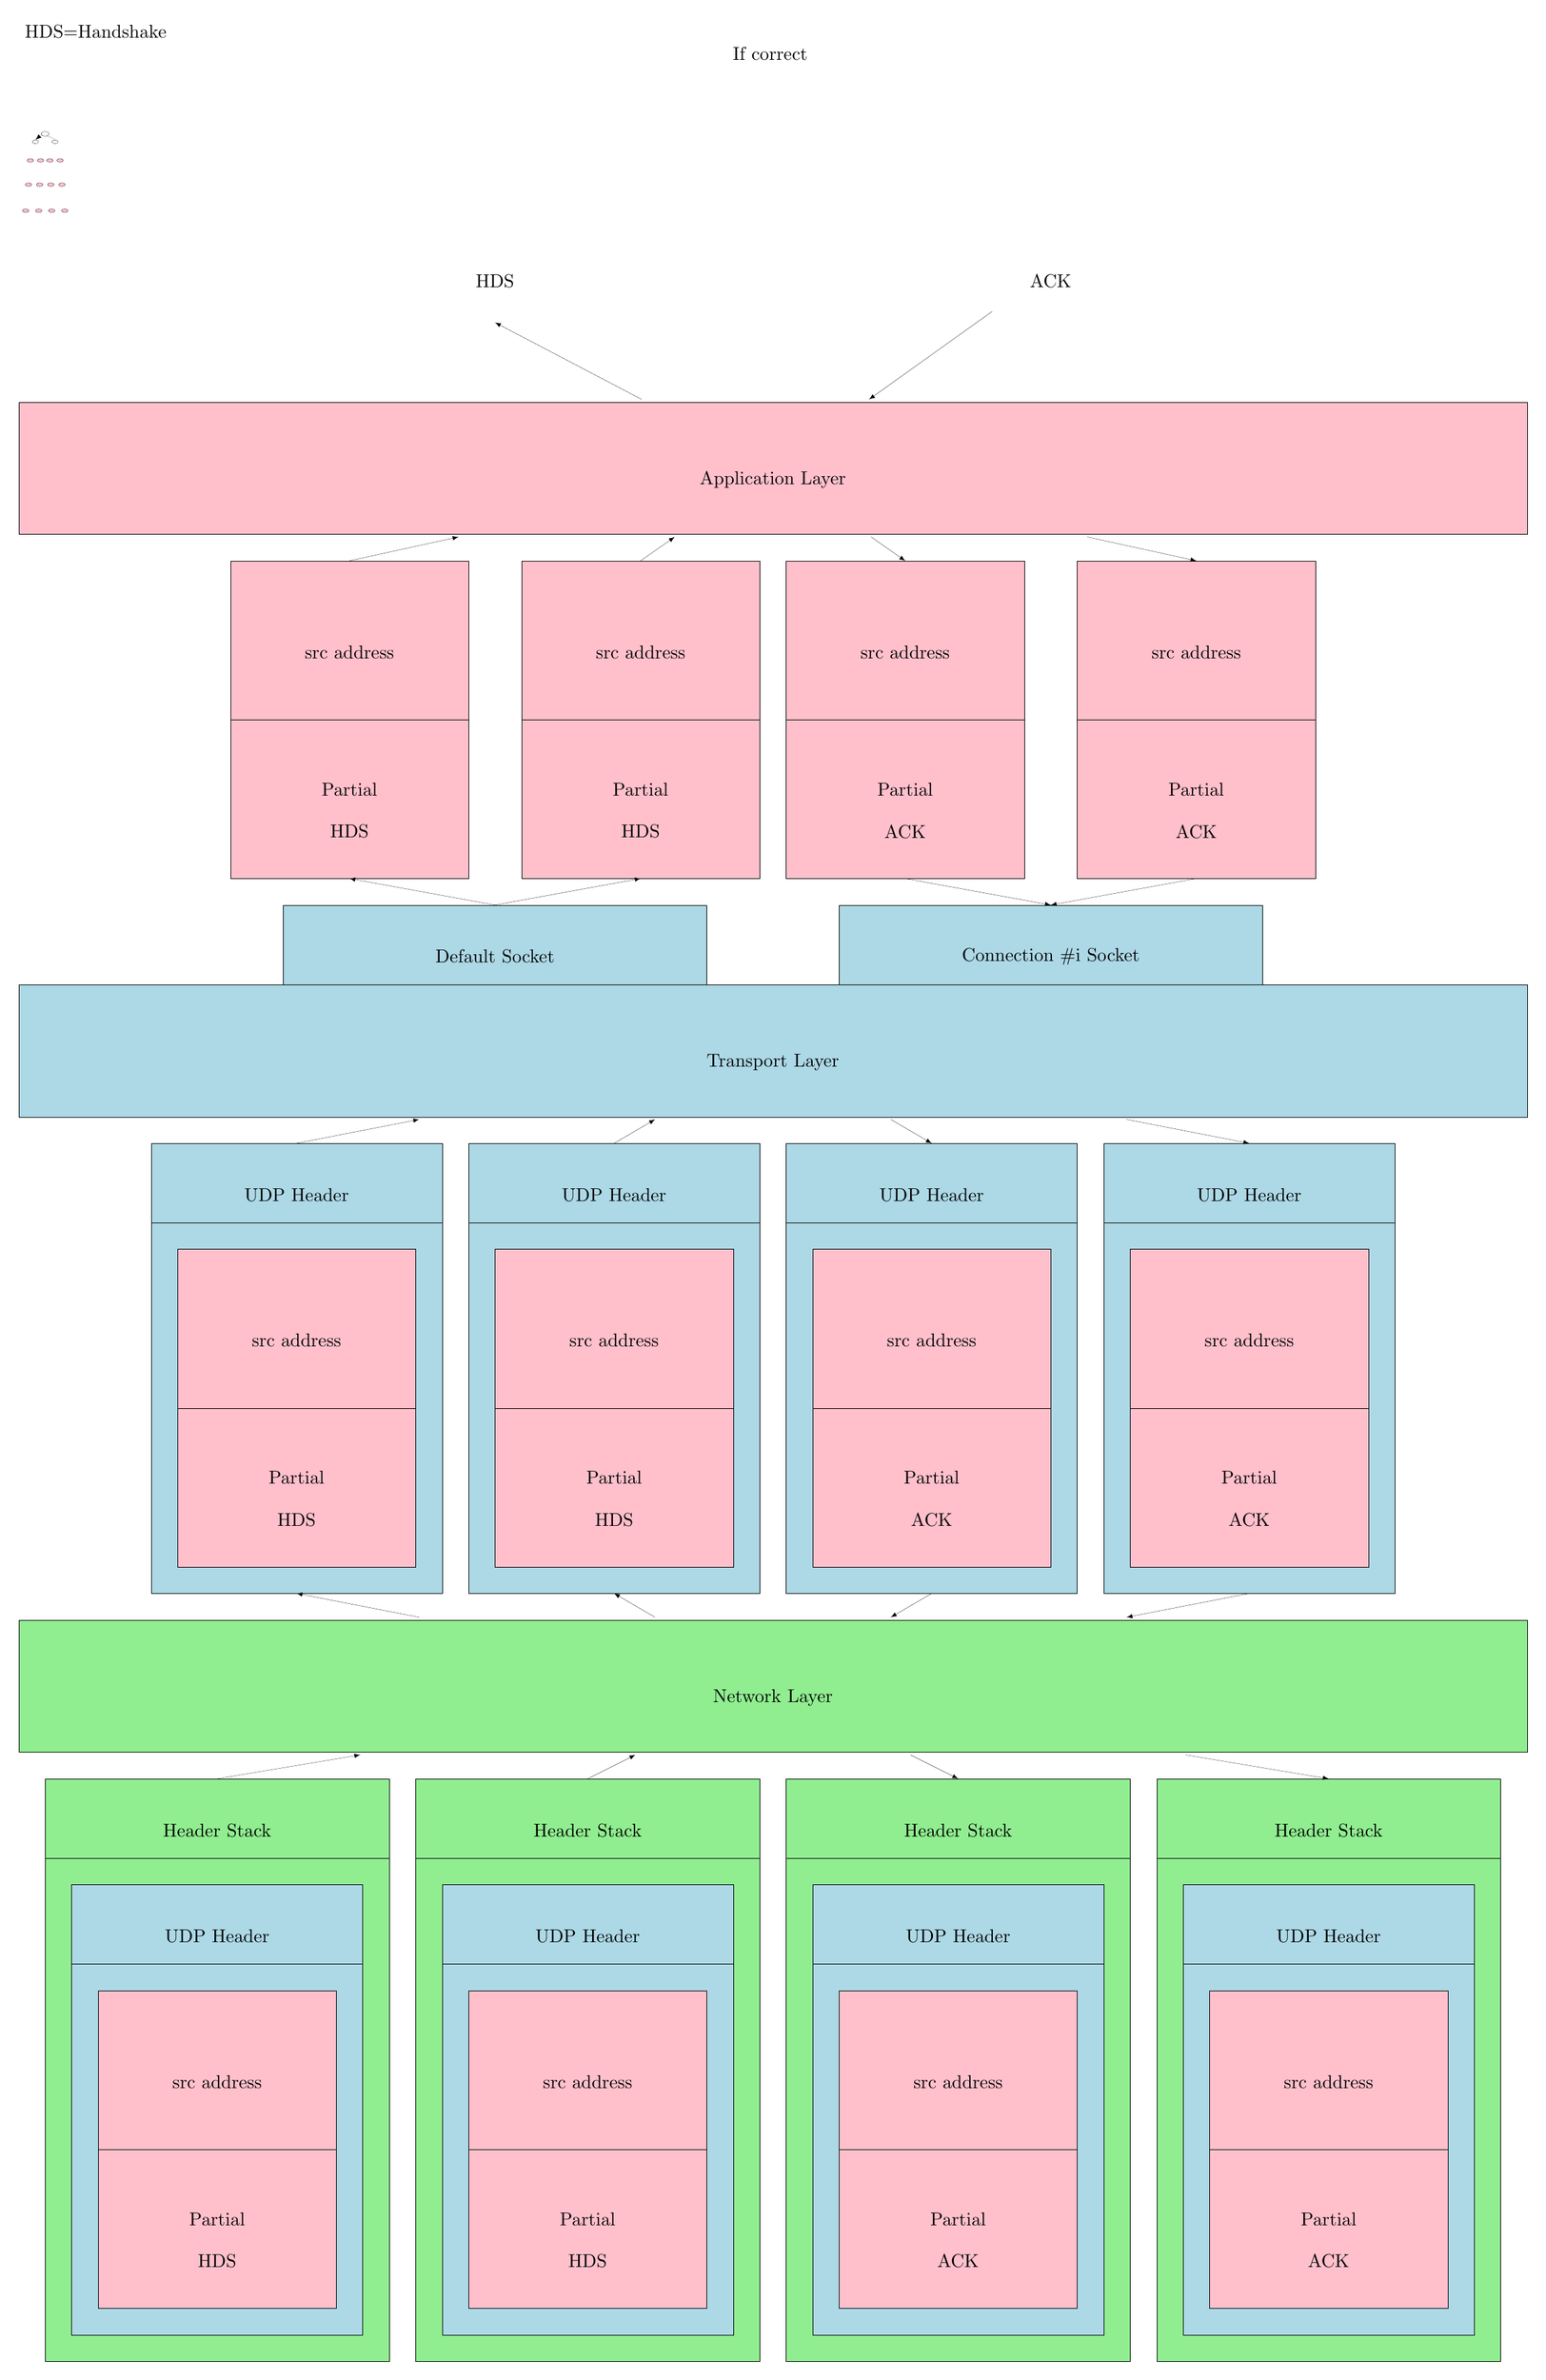
\begin{tikzpicture}
\pgftransformxscale{1.000000}
\pgftransformyscale{-1.000000}
\definecolor{dialinecolor}{rgb}{0.000000, 0.000000, 0.000000}
\pgfsetstrokecolor{dialinecolor}
\definecolor{dialinecolor}{rgb}{1.000000, 1.000000, 1.000000}
\pgfsetfillcolor{dialinecolor}
\pgfsetlinewidth{0.100000\du}
\pgfsetdash{}{0pt}
\pgfsetdash{}{0pt}
\pgfsetmiterjoin
\definecolor{dialinecolor}{rgb}{0.564706, 0.933333, 0.564706}
\pgfsetfillcolor{dialinecolor}
\fill (7.500000\du,32.500000\du)--(7.500000\du,42.000000\du)--(14.000000\du,42.000000\du)--(14.000000\du,32.500000\du)--cycle;
\definecolor{dialinecolor}{rgb}{0.000000, 0.000000, 0.000000}
\pgfsetstrokecolor{dialinecolor}
\draw (7.500000\du,32.500000\du)--(7.500000\du,42.000000\du)--(14.000000\du,42.000000\du)--(14.000000\du,32.500000\du)--cycle;
\pgfsetlinewidth{0.100000\du}
\pgfsetdash{}{0pt}
\pgfsetdash{}{0pt}
\pgfsetmiterjoin
\definecolor{dialinecolor}{rgb}{0.564706, 0.933333, 0.564706}
\pgfsetfillcolor{dialinecolor}
\fill (0.500000\du,32.500000\du)--(0.500000\du,42.000000\du)--(7.000000\du,42.000000\du)--(7.000000\du,32.500000\du)--cycle;
\definecolor{dialinecolor}{rgb}{0.000000, 0.000000, 0.000000}
\pgfsetstrokecolor{dialinecolor}
\draw (0.500000\du,32.500000\du)--(0.500000\du,42.000000\du)--(7.000000\du,42.000000\du)--(7.000000\du,32.500000\du)--cycle;
\pgfsetlinewidth{0.100000\du}
\pgfsetdash{}{0pt}
\pgfsetdash{}{0pt}
\pgfsetmiterjoin
\definecolor{dialinecolor}{rgb}{0.678431, 0.847059, 0.901961}
\pgfsetfillcolor{dialinecolor}
\fill (0.000000\du,16.000000\du)--(0.000000\du,18.500000\du)--(28.500000\du,18.500000\du)--(28.500000\du,16.000000\du)--cycle;
\definecolor{dialinecolor}{rgb}{0.000000, 0.000000, 0.000000}
\pgfsetstrokecolor{dialinecolor}
\draw (0.000000\du,16.000000\du)--(0.000000\du,18.500000\du)--(28.500000\du,18.500000\du)--(28.500000\du,16.000000\du)--cycle;
% setfont left to latex
\definecolor{dialinecolor}{rgb}{0.000000, 0.000000, 0.000000}
\pgfsetstrokecolor{dialinecolor}
\node at (14.250000\du,17.472500\du){Transport Layer};
\pgfsetlinewidth{0.100000\du}
\pgfsetdash{}{0pt}
\pgfsetdash{}{0pt}
\pgfsetmiterjoin
\definecolor{dialinecolor}{rgb}{0.564706, 0.933333, 0.564706}
\pgfsetfillcolor{dialinecolor}
\fill (0.000000\du,28.000000\du)--(0.000000\du,30.500000\du)--(28.500000\du,30.500000\du)--(28.500000\du,28.000000\du)--cycle;
\definecolor{dialinecolor}{rgb}{0.000000, 0.000000, 0.000000}
\pgfsetstrokecolor{dialinecolor}
\draw (0.000000\du,28.000000\du)--(0.000000\du,30.500000\du)--(28.500000\du,30.500000\du)--(28.500000\du,28.000000\du)--cycle;
% setfont left to latex
\definecolor{dialinecolor}{rgb}{0.000000, 0.000000, 0.000000}
\pgfsetstrokecolor{dialinecolor}
\node at (14.250000\du,29.472500\du){Network Layer};
\pgfsetlinewidth{0.100000\du}
\pgfsetdash{}{0pt}
\pgfsetdash{}{0pt}
\pgfsetmiterjoin
\definecolor{dialinecolor}{rgb}{1.000000, 0.752941, 0.796078}
\pgfsetfillcolor{dialinecolor}
\fill (0.000000\du,5.000000\du)--(0.000000\du,7.500000\du)--(28.500000\du,7.500000\du)--(28.500000\du,5.000000\du)--cycle;
\definecolor{dialinecolor}{rgb}{0.000000, 0.000000, 0.000000}
\pgfsetstrokecolor{dialinecolor}
\draw (0.000000\du,5.000000\du)--(0.000000\du,7.500000\du)--(28.500000\du,7.500000\du)--(28.500000\du,5.000000\du)--cycle;
% setfont left to latex
\definecolor{dialinecolor}{rgb}{0.000000, 0.000000, 0.000000}
\pgfsetstrokecolor{dialinecolor}
\node at (14.250000\du,6.472500\du){Application Layer};
\definecolor{dialinecolor}{rgb}{1.000000, 1.000000, 1.000000}
\pgfsetfillcolor{dialinecolor}
\pgfpathellipse{\pgfpoint{9.000000\du}{2.500000\du}}{\pgfpoint{1.650000\du}{0\du}}{\pgfpoint{0\du}{1.000000\du}}
\pgfusepath{fill}
\pgfsetlinewidth{0.100000\du}
\pgfsetdash{}{0pt}
\pgfsetdash{}{0pt}
\definecolor{dialinecolor}{rgb}{0.000000, 0.000000, 0.000000}
\pgfsetstrokecolor{dialinecolor}
\pgfpathellipse{\pgfpoint{9.000000\du}{2.500000\du}}{\pgfpoint{1.650000\du}{0\du}}{\pgfpoint{0\du}{1.000000\du}}
\pgfusepath{stroke}
% setfont left to latex
\definecolor{dialinecolor}{rgb}{0.000000, 0.000000, 0.000000}
\pgfsetstrokecolor{dialinecolor}
\node at (9.000000\du,2.713188\du){HDS};
\pgfsetlinewidth{0.100000\du}
\pgfsetdash{}{0pt}
\pgfsetdash{}{0pt}
\pgfsetmiterjoin
\definecolor{dialinecolor}{rgb}{0.678431, 0.847059, 0.901961}
\pgfsetfillcolor{dialinecolor}
\fill (8.500000\du,20.500000\du)--(8.500000\du,27.500000\du)--(14.000000\du,27.500000\du)--(14.000000\du,20.500000\du)--cycle;
\definecolor{dialinecolor}{rgb}{0.000000, 0.000000, 0.000000}
\pgfsetstrokecolor{dialinecolor}
\draw (8.500000\du,20.500000\du)--(8.500000\du,27.500000\du)--(14.000000\du,27.500000\du)--(14.000000\du,20.500000\du)--cycle;
\pgfsetlinewidth{0.100000\du}
\pgfsetdash{}{0pt}
\pgfsetdash{}{0pt}
\pgfsetmiterjoin
\definecolor{dialinecolor}{rgb}{1.000000, 0.752941, 0.796078}
\pgfsetfillcolor{dialinecolor}
\fill (9.000000\du,24.000000\du)--(9.000000\du,27.000000\du)--(13.500000\du,27.000000\du)--(13.500000\du,24.000000\du)--cycle;
\definecolor{dialinecolor}{rgb}{0.000000, 0.000000, 0.000000}
\pgfsetstrokecolor{dialinecolor}
\draw (9.000000\du,24.000000\du)--(9.000000\du,27.000000\du)--(13.500000\du,27.000000\du)--(13.500000\du,24.000000\du)--cycle;
\definecolor{dialinecolor}{rgb}{1.000000, 0.752941, 0.796078}
\pgfsetfillcolor{dialinecolor}
\pgfpathellipse{\pgfpoint{11.250000\du}{25.500000\du}}{\pgfpoint{1.750000\du}{0\du}}{\pgfpoint{0\du}{1.000000\du}}
\pgfusepath{fill}
\pgfsetlinewidth{0.100000\du}
\pgfsetdash{}{0pt}
\pgfsetdash{}{0pt}
\definecolor{dialinecolor}{rgb}{0.000000, 0.000000, 0.000000}
\pgfsetstrokecolor{dialinecolor}
\pgfpathellipse{\pgfpoint{11.250000\du}{25.500000\du}}{\pgfpoint{1.750000\du}{0\du}}{\pgfpoint{0\du}{1.000000\du}}
\pgfusepath{stroke}
\pgfsetlinewidth{0.100000\du}
\pgfsetdash{}{0pt}
\pgfsetdash{}{0pt}
\pgfsetmiterjoin
\definecolor{dialinecolor}{rgb}{1.000000, 0.752941, 0.796078}
\pgfsetfillcolor{dialinecolor}
\fill (9.000000\du,21.000000\du)--(9.000000\du,24.000000\du)--(13.500000\du,24.000000\du)--(13.500000\du,21.000000\du)--cycle;
\definecolor{dialinecolor}{rgb}{0.000000, 0.000000, 0.000000}
\pgfsetstrokecolor{dialinecolor}
\draw (9.000000\du,21.000000\du)--(9.000000\du,24.000000\du)--(13.500000\du,24.000000\du)--(13.500000\du,21.000000\du)--cycle;
% setfont left to latex
\definecolor{dialinecolor}{rgb}{0.000000, 0.000000, 0.000000}
\pgfsetstrokecolor{dialinecolor}
\node at (11.250000\du,22.722500\du){src address};
\pgfsetlinewidth{0.100000\du}
\pgfsetdash{}{0pt}
\pgfsetdash{}{0pt}
\pgfsetmiterjoin
\definecolor{dialinecolor}{rgb}{0.678431, 0.847059, 0.901961}
\pgfsetfillcolor{dialinecolor}
\fill (8.500000\du,19.000000\du)--(8.500000\du,20.500000\du)--(14.000000\du,20.500000\du)--(14.000000\du,19.000000\du)--cycle;
\definecolor{dialinecolor}{rgb}{0.000000, 0.000000, 0.000000}
\pgfsetstrokecolor{dialinecolor}
\draw (8.500000\du,19.000000\du)--(8.500000\du,20.500000\du)--(14.000000\du,20.500000\du)--(14.000000\du,19.000000\du)--cycle;
% setfont left to latex
\definecolor{dialinecolor}{rgb}{0.000000, 0.000000, 0.000000}
\pgfsetstrokecolor{dialinecolor}
\node at (11.250000\du,19.972500\du){UDP Header};
\pgfsetlinewidth{0.100000\du}
\pgfsetdash{}{0pt}
\pgfsetdash{}{0pt}
\pgfsetmiterjoin
\definecolor{dialinecolor}{rgb}{0.678431, 0.847059, 0.901961}
\pgfsetfillcolor{dialinecolor}
\fill (2.500000\du,20.500000\du)--(2.500000\du,27.500000\du)--(8.000000\du,27.500000\du)--(8.000000\du,20.500000\du)--cycle;
\definecolor{dialinecolor}{rgb}{0.000000, 0.000000, 0.000000}
\pgfsetstrokecolor{dialinecolor}
\draw (2.500000\du,20.500000\du)--(2.500000\du,27.500000\du)--(8.000000\du,27.500000\du)--(8.000000\du,20.500000\du)--cycle;
\pgfsetlinewidth{0.100000\du}
\pgfsetdash{}{0pt}
\pgfsetdash{}{0pt}
\pgfsetmiterjoin
\definecolor{dialinecolor}{rgb}{1.000000, 0.752941, 0.796078}
\pgfsetfillcolor{dialinecolor}
\fill (3.000000\du,24.000000\du)--(3.000000\du,27.000000\du)--(7.500000\du,27.000000\du)--(7.500000\du,24.000000\du)--cycle;
\definecolor{dialinecolor}{rgb}{0.000000, 0.000000, 0.000000}
\pgfsetstrokecolor{dialinecolor}
\draw (3.000000\du,24.000000\du)--(3.000000\du,27.000000\du)--(7.500000\du,27.000000\du)--(7.500000\du,24.000000\du)--cycle;
\definecolor{dialinecolor}{rgb}{1.000000, 0.752941, 0.796078}
\pgfsetfillcolor{dialinecolor}
\pgfpathellipse{\pgfpoint{5.250000\du}{25.500000\du}}{\pgfpoint{1.750000\du}{0\du}}{\pgfpoint{0\du}{1.000000\du}}
\pgfusepath{fill}
\pgfsetlinewidth{0.100000\du}
\pgfsetdash{}{0pt}
\pgfsetdash{}{0pt}
\definecolor{dialinecolor}{rgb}{0.000000, 0.000000, 0.000000}
\pgfsetstrokecolor{dialinecolor}
\pgfpathellipse{\pgfpoint{5.250000\du}{25.500000\du}}{\pgfpoint{1.750000\du}{0\du}}{\pgfpoint{0\du}{1.000000\du}}
\pgfusepath{stroke}
\pgfsetlinewidth{0.100000\du}
\pgfsetdash{}{0pt}
\pgfsetdash{}{0pt}
\pgfsetmiterjoin
\definecolor{dialinecolor}{rgb}{1.000000, 0.752941, 0.796078}
\pgfsetfillcolor{dialinecolor}
\fill (3.000000\du,21.000000\du)--(3.000000\du,24.000000\du)--(7.500000\du,24.000000\du)--(7.500000\du,21.000000\du)--cycle;
\definecolor{dialinecolor}{rgb}{0.000000, 0.000000, 0.000000}
\pgfsetstrokecolor{dialinecolor}
\draw (3.000000\du,21.000000\du)--(3.000000\du,24.000000\du)--(7.500000\du,24.000000\du)--(7.500000\du,21.000000\du)--cycle;
% setfont left to latex
\definecolor{dialinecolor}{rgb}{0.000000, 0.000000, 0.000000}
\pgfsetstrokecolor{dialinecolor}
\node at (5.250000\du,22.722500\du){src address};
\pgfsetlinewidth{0.100000\du}
\pgfsetdash{}{0pt}
\pgfsetdash{}{0pt}
\pgfsetmiterjoin
\definecolor{dialinecolor}{rgb}{0.678431, 0.847059, 0.901961}
\pgfsetfillcolor{dialinecolor}
\fill (2.500000\du,19.000000\du)--(2.500000\du,20.500000\du)--(8.000000\du,20.500000\du)--(8.000000\du,19.000000\du)--cycle;
\definecolor{dialinecolor}{rgb}{0.000000, 0.000000, 0.000000}
\pgfsetstrokecolor{dialinecolor}
\draw (2.500000\du,19.000000\du)--(2.500000\du,20.500000\du)--(8.000000\du,20.500000\du)--(8.000000\du,19.000000\du)--cycle;
% setfont left to latex
\definecolor{dialinecolor}{rgb}{0.000000, 0.000000, 0.000000}
\pgfsetstrokecolor{dialinecolor}
\node at (5.250000\du,19.972500\du){UDP Header};
\pgfsetlinewidth{0.100000\du}
\pgfsetdash{}{0pt}
\pgfsetdash{}{0pt}
\pgfsetmiterjoin
\definecolor{dialinecolor}{rgb}{0.678431, 0.847059, 0.901961}
\pgfsetfillcolor{dialinecolor}
\fill (1.000000\du,34.500000\du)--(1.000000\du,41.500000\du)--(6.500000\du,41.500000\du)--(6.500000\du,34.500000\du)--cycle;
\definecolor{dialinecolor}{rgb}{0.000000, 0.000000, 0.000000}
\pgfsetstrokecolor{dialinecolor}
\draw (1.000000\du,34.500000\du)--(1.000000\du,41.500000\du)--(6.500000\du,41.500000\du)--(6.500000\du,34.500000\du)--cycle;
\pgfsetlinewidth{0.100000\du}
\pgfsetdash{}{0pt}
\pgfsetdash{}{0pt}
\pgfsetmiterjoin
\definecolor{dialinecolor}{rgb}{1.000000, 0.752941, 0.796078}
\pgfsetfillcolor{dialinecolor}
\fill (1.500000\du,38.000000\du)--(1.500000\du,41.000000\du)--(6.000000\du,41.000000\du)--(6.000000\du,38.000000\du)--cycle;
\definecolor{dialinecolor}{rgb}{0.000000, 0.000000, 0.000000}
\pgfsetstrokecolor{dialinecolor}
\draw (1.500000\du,38.000000\du)--(1.500000\du,41.000000\du)--(6.000000\du,41.000000\du)--(6.000000\du,38.000000\du)--cycle;
\definecolor{dialinecolor}{rgb}{1.000000, 0.752941, 0.796078}
\pgfsetfillcolor{dialinecolor}
\pgfpathellipse{\pgfpoint{3.750000\du}{39.500000\du}}{\pgfpoint{1.750000\du}{0\du}}{\pgfpoint{0\du}{1.000000\du}}
\pgfusepath{fill}
\pgfsetlinewidth{0.100000\du}
\pgfsetdash{}{0pt}
\pgfsetdash{}{0pt}
\definecolor{dialinecolor}{rgb}{0.000000, 0.000000, 0.000000}
\pgfsetstrokecolor{dialinecolor}
\pgfpathellipse{\pgfpoint{3.750000\du}{39.500000\du}}{\pgfpoint{1.750000\du}{0\du}}{\pgfpoint{0\du}{1.000000\du}}
\pgfusepath{stroke}
\pgfsetlinewidth{0.100000\du}
\pgfsetdash{}{0pt}
\pgfsetdash{}{0pt}
\pgfsetmiterjoin
\definecolor{dialinecolor}{rgb}{1.000000, 0.752941, 0.796078}
\pgfsetfillcolor{dialinecolor}
\fill (1.500000\du,35.000000\du)--(1.500000\du,38.000000\du)--(6.000000\du,38.000000\du)--(6.000000\du,35.000000\du)--cycle;
\definecolor{dialinecolor}{rgb}{0.000000, 0.000000, 0.000000}
\pgfsetstrokecolor{dialinecolor}
\draw (1.500000\du,35.000000\du)--(1.500000\du,38.000000\du)--(6.000000\du,38.000000\du)--(6.000000\du,35.000000\du)--cycle;
% setfont left to latex
\definecolor{dialinecolor}{rgb}{0.000000, 0.000000, 0.000000}
\pgfsetstrokecolor{dialinecolor}
\node at (3.750000\du,36.722500\du){src address};
\pgfsetlinewidth{0.100000\du}
\pgfsetdash{}{0pt}
\pgfsetdash{}{0pt}
\pgfsetmiterjoin
\definecolor{dialinecolor}{rgb}{0.678431, 0.847059, 0.901961}
\pgfsetfillcolor{dialinecolor}
\fill (1.000000\du,33.000000\du)--(1.000000\du,34.500000\du)--(6.500000\du,34.500000\du)--(6.500000\du,33.000000\du)--cycle;
\definecolor{dialinecolor}{rgb}{0.000000, 0.000000, 0.000000}
\pgfsetstrokecolor{dialinecolor}
\draw (1.000000\du,33.000000\du)--(1.000000\du,34.500000\du)--(6.500000\du,34.500000\du)--(6.500000\du,33.000000\du)--cycle;
% setfont left to latex
\definecolor{dialinecolor}{rgb}{0.000000, 0.000000, 0.000000}
\pgfsetstrokecolor{dialinecolor}
\node at (3.750000\du,33.972500\du){UDP Header};
\pgfsetlinewidth{0.100000\du}
\pgfsetdash{}{0pt}
\pgfsetdash{}{0pt}
\pgfsetmiterjoin
\definecolor{dialinecolor}{rgb}{0.678431, 0.847059, 0.901961}
\pgfsetfillcolor{dialinecolor}
\fill (8.000000\du,34.500000\du)--(8.000000\du,41.500000\du)--(13.500000\du,41.500000\du)--(13.500000\du,34.500000\du)--cycle;
\definecolor{dialinecolor}{rgb}{0.000000, 0.000000, 0.000000}
\pgfsetstrokecolor{dialinecolor}
\draw (8.000000\du,34.500000\du)--(8.000000\du,41.500000\du)--(13.500000\du,41.500000\du)--(13.500000\du,34.500000\du)--cycle;
\pgfsetlinewidth{0.100000\du}
\pgfsetdash{}{0pt}
\pgfsetdash{}{0pt}
\pgfsetmiterjoin
\definecolor{dialinecolor}{rgb}{1.000000, 0.752941, 0.796078}
\pgfsetfillcolor{dialinecolor}
\fill (8.500000\du,38.000000\du)--(8.500000\du,41.000000\du)--(13.000000\du,41.000000\du)--(13.000000\du,38.000000\du)--cycle;
\definecolor{dialinecolor}{rgb}{0.000000, 0.000000, 0.000000}
\pgfsetstrokecolor{dialinecolor}
\draw (8.500000\du,38.000000\du)--(8.500000\du,41.000000\du)--(13.000000\du,41.000000\du)--(13.000000\du,38.000000\du)--cycle;
\definecolor{dialinecolor}{rgb}{1.000000, 0.752941, 0.796078}
\pgfsetfillcolor{dialinecolor}
\pgfpathellipse{\pgfpoint{10.750000\du}{39.500000\du}}{\pgfpoint{1.750000\du}{0\du}}{\pgfpoint{0\du}{1.000000\du}}
\pgfusepath{fill}
\pgfsetlinewidth{0.100000\du}
\pgfsetdash{}{0pt}
\pgfsetdash{}{0pt}
\definecolor{dialinecolor}{rgb}{0.000000, 0.000000, 0.000000}
\pgfsetstrokecolor{dialinecolor}
\pgfpathellipse{\pgfpoint{10.750000\du}{39.500000\du}}{\pgfpoint{1.750000\du}{0\du}}{\pgfpoint{0\du}{1.000000\du}}
\pgfusepath{stroke}
\pgfsetlinewidth{0.100000\du}
\pgfsetdash{}{0pt}
\pgfsetdash{}{0pt}
\pgfsetmiterjoin
\definecolor{dialinecolor}{rgb}{1.000000, 0.752941, 0.796078}
\pgfsetfillcolor{dialinecolor}
\fill (8.500000\du,35.000000\du)--(8.500000\du,38.000000\du)--(13.000000\du,38.000000\du)--(13.000000\du,35.000000\du)--cycle;
\definecolor{dialinecolor}{rgb}{0.000000, 0.000000, 0.000000}
\pgfsetstrokecolor{dialinecolor}
\draw (8.500000\du,35.000000\du)--(8.500000\du,38.000000\du)--(13.000000\du,38.000000\du)--(13.000000\du,35.000000\du)--cycle;
% setfont left to latex
\definecolor{dialinecolor}{rgb}{0.000000, 0.000000, 0.000000}
\pgfsetstrokecolor{dialinecolor}
\node at (10.750000\du,36.722500\du){src address};
\pgfsetlinewidth{0.100000\du}
\pgfsetdash{}{0pt}
\pgfsetdash{}{0pt}
\pgfsetmiterjoin
\definecolor{dialinecolor}{rgb}{0.678431, 0.847059, 0.901961}
\pgfsetfillcolor{dialinecolor}
\fill (8.000000\du,33.000000\du)--(8.000000\du,34.500000\du)--(13.500000\du,34.500000\du)--(13.500000\du,33.000000\du)--cycle;
\definecolor{dialinecolor}{rgb}{0.000000, 0.000000, 0.000000}
\pgfsetstrokecolor{dialinecolor}
\draw (8.000000\du,33.000000\du)--(8.000000\du,34.500000\du)--(13.500000\du,34.500000\du)--(13.500000\du,33.000000\du)--cycle;
% setfont left to latex
\definecolor{dialinecolor}{rgb}{0.000000, 0.000000, 0.000000}
\pgfsetstrokecolor{dialinecolor}
\node at (10.750000\du,33.972500\du){UDP Header};
\pgfsetlinewidth{0.100000\du}
\pgfsetdash{}{0pt}
\pgfsetdash{}{0pt}
\pgfsetmiterjoin
\definecolor{dialinecolor}{rgb}{0.564706, 0.933333, 0.564706}
\pgfsetfillcolor{dialinecolor}
\fill (0.500000\du,31.000000\du)--(0.500000\du,32.500000\du)--(7.000000\du,32.500000\du)--(7.000000\du,31.000000\du)--cycle;
\definecolor{dialinecolor}{rgb}{0.000000, 0.000000, 0.000000}
\pgfsetstrokecolor{dialinecolor}
\draw (0.500000\du,31.000000\du)--(0.500000\du,32.500000\du)--(7.000000\du,32.500000\du)--(7.000000\du,31.000000\du)--cycle;
% setfont left to latex
\definecolor{dialinecolor}{rgb}{0.000000, 0.000000, 0.000000}
\pgfsetstrokecolor{dialinecolor}
\node at (3.750000\du,31.972500\du){Header Stack};
\pgfsetlinewidth{0.100000\du}
\pgfsetdash{}{0pt}
\pgfsetdash{}{0pt}
\pgfsetmiterjoin
\definecolor{dialinecolor}{rgb}{0.564706, 0.933333, 0.564706}
\pgfsetfillcolor{dialinecolor}
\fill (7.500000\du,31.000000\du)--(7.500000\du,32.500000\du)--(14.000000\du,32.500000\du)--(14.000000\du,31.000000\du)--cycle;
\definecolor{dialinecolor}{rgb}{0.000000, 0.000000, 0.000000}
\pgfsetstrokecolor{dialinecolor}
\draw (7.500000\du,31.000000\du)--(7.500000\du,32.500000\du)--(14.000000\du,32.500000\du)--(14.000000\du,31.000000\du)--cycle;
% setfont left to latex
\definecolor{dialinecolor}{rgb}{0.000000, 0.000000, 0.000000}
\pgfsetstrokecolor{dialinecolor}
\node at (10.750000\du,31.972500\du){Header Stack};
\pgfsetlinewidth{0.100000\du}
\pgfsetdash{}{0pt}
\pgfsetdash{}{0pt}
\pgfsetmiterjoin
\definecolor{dialinecolor}{rgb}{1.000000, 0.752941, 0.796078}
\pgfsetfillcolor{dialinecolor}
\fill (9.500000\du,11.000000\du)--(9.500000\du,14.000000\du)--(14.000000\du,14.000000\du)--(14.000000\du,11.000000\du)--cycle;
\definecolor{dialinecolor}{rgb}{0.000000, 0.000000, 0.000000}
\pgfsetstrokecolor{dialinecolor}
\draw (9.500000\du,11.000000\du)--(9.500000\du,14.000000\du)--(14.000000\du,14.000000\du)--(14.000000\du,11.000000\du)--cycle;
\definecolor{dialinecolor}{rgb}{1.000000, 0.752941, 0.796078}
\pgfsetfillcolor{dialinecolor}
\pgfpathellipse{\pgfpoint{11.750000\du}{12.500000\du}}{\pgfpoint{1.750000\du}{0\du}}{\pgfpoint{0\du}{1.000000\du}}
\pgfusepath{fill}
\pgfsetlinewidth{0.100000\du}
\pgfsetdash{}{0pt}
\pgfsetdash{}{0pt}
\definecolor{dialinecolor}{rgb}{0.000000, 0.000000, 0.000000}
\pgfsetstrokecolor{dialinecolor}
\pgfpathellipse{\pgfpoint{11.750000\du}{12.500000\du}}{\pgfpoint{1.750000\du}{0\du}}{\pgfpoint{0\du}{1.000000\du}}
\pgfusepath{stroke}
\pgfsetlinewidth{0.100000\du}
\pgfsetdash{}{0pt}
\pgfsetdash{}{0pt}
\pgfsetmiterjoin
\definecolor{dialinecolor}{rgb}{1.000000, 0.752941, 0.796078}
\pgfsetfillcolor{dialinecolor}
\fill (9.500000\du,8.000000\du)--(9.500000\du,11.000000\du)--(14.000000\du,11.000000\du)--(14.000000\du,8.000000\du)--cycle;
\definecolor{dialinecolor}{rgb}{0.000000, 0.000000, 0.000000}
\pgfsetstrokecolor{dialinecolor}
\draw (9.500000\du,8.000000\du)--(9.500000\du,11.000000\du)--(14.000000\du,11.000000\du)--(14.000000\du,8.000000\du)--cycle;
% setfont left to latex
\definecolor{dialinecolor}{rgb}{0.000000, 0.000000, 0.000000}
\pgfsetstrokecolor{dialinecolor}
\node at (11.750000\du,9.722500\du){src address};
% setfont left to latex
\definecolor{dialinecolor}{rgb}{0.000000, 0.000000, 0.000000}
\pgfsetstrokecolor{dialinecolor}
\node at (11.750000\du,12.313188\du){Partial};
% setfont left to latex
\definecolor{dialinecolor}{rgb}{0.000000, 0.000000, 0.000000}
\pgfsetstrokecolor{dialinecolor}
\node at (11.750000\du,13.113188\du){HDS};
\pgfsetlinewidth{0.100000\du}
\pgfsetdash{}{0pt}
\pgfsetdash{}{0pt}
\pgfsetmiterjoin
\definecolor{dialinecolor}{rgb}{1.000000, 0.752941, 0.796078}
\pgfsetfillcolor{dialinecolor}
\fill (4.000000\du,11.000000\du)--(4.000000\du,14.000000\du)--(8.500000\du,14.000000\du)--(8.500000\du,11.000000\du)--cycle;
\definecolor{dialinecolor}{rgb}{0.000000, 0.000000, 0.000000}
\pgfsetstrokecolor{dialinecolor}
\draw (4.000000\du,11.000000\du)--(4.000000\du,14.000000\du)--(8.500000\du,14.000000\du)--(8.500000\du,11.000000\du)--cycle;
\definecolor{dialinecolor}{rgb}{1.000000, 0.752941, 0.796078}
\pgfsetfillcolor{dialinecolor}
\pgfpathellipse{\pgfpoint{6.250000\du}{12.500000\du}}{\pgfpoint{1.750000\du}{0\du}}{\pgfpoint{0\du}{1.000000\du}}
\pgfusepath{fill}
\pgfsetlinewidth{0.100000\du}
\pgfsetdash{}{0pt}
\pgfsetdash{}{0pt}
\definecolor{dialinecolor}{rgb}{0.000000, 0.000000, 0.000000}
\pgfsetstrokecolor{dialinecolor}
\pgfpathellipse{\pgfpoint{6.250000\du}{12.500000\du}}{\pgfpoint{1.750000\du}{0\du}}{\pgfpoint{0\du}{1.000000\du}}
\pgfusepath{stroke}
\pgfsetlinewidth{0.100000\du}
\pgfsetdash{}{0pt}
\pgfsetdash{}{0pt}
\pgfsetmiterjoin
\definecolor{dialinecolor}{rgb}{1.000000, 0.752941, 0.796078}
\pgfsetfillcolor{dialinecolor}
\fill (4.000000\du,8.000000\du)--(4.000000\du,11.000000\du)--(8.500000\du,11.000000\du)--(8.500000\du,8.000000\du)--cycle;
\definecolor{dialinecolor}{rgb}{0.000000, 0.000000, 0.000000}
\pgfsetstrokecolor{dialinecolor}
\draw (4.000000\du,8.000000\du)--(4.000000\du,11.000000\du)--(8.500000\du,11.000000\du)--(8.500000\du,8.000000\du)--cycle;
% setfont left to latex
\definecolor{dialinecolor}{rgb}{0.000000, 0.000000, 0.000000}
\pgfsetstrokecolor{dialinecolor}
\node at (6.250000\du,9.722500\du){src address};
% setfont left to latex
\definecolor{dialinecolor}{rgb}{0.000000, 0.000000, 0.000000}
\pgfsetstrokecolor{dialinecolor}
\node at (6.250000\du,12.313188\du){Partial};
% setfont left to latex
\definecolor{dialinecolor}{rgb}{0.000000, 0.000000, 0.000000}
\pgfsetstrokecolor{dialinecolor}
\node at (6.250000\du,13.113188\du){HDS};
% setfont left to latex
\definecolor{dialinecolor}{rgb}{0.000000, 0.000000, 0.000000}
\pgfsetstrokecolor{dialinecolor}
\node at (5.250000\du,25.313187\du){Partial};
% setfont left to latex
\definecolor{dialinecolor}{rgb}{0.000000, 0.000000, 0.000000}
\pgfsetstrokecolor{dialinecolor}
\node at (5.250000\du,26.113187\du){HDS};
% setfont left to latex
\definecolor{dialinecolor}{rgb}{0.000000, 0.000000, 0.000000}
\pgfsetstrokecolor{dialinecolor}
\node at (11.250000\du,25.313187\du){Partial};
% setfont left to latex
\definecolor{dialinecolor}{rgb}{0.000000, 0.000000, 0.000000}
\pgfsetstrokecolor{dialinecolor}
\node at (11.250000\du,26.113187\du){HDS};
% setfont left to latex
\definecolor{dialinecolor}{rgb}{0.000000, 0.000000, 0.000000}
\pgfsetstrokecolor{dialinecolor}
\node at (10.750000\du,39.313187\du){Partial};
% setfont left to latex
\definecolor{dialinecolor}{rgb}{0.000000, 0.000000, 0.000000}
\pgfsetstrokecolor{dialinecolor}
\node at (10.750000\du,40.113187\du){HDS};
% setfont left to latex
\definecolor{dialinecolor}{rgb}{0.000000, 0.000000, 0.000000}
\pgfsetstrokecolor{dialinecolor}
\node at (3.750000\du,39.313187\du){Partial};
% setfont left to latex
\definecolor{dialinecolor}{rgb}{0.000000, 0.000000, 0.000000}
\pgfsetstrokecolor{dialinecolor}
\node at (3.750000\du,40.113187\du){HDS};
\pgfsetlinewidth{0.100000\du}
\pgfsetdash{}{0pt}
\pgfsetdash{}{0pt}
\pgfsetmiterjoin
\definecolor{dialinecolor}{rgb}{0.678431, 0.847059, 0.901961}
\pgfsetfillcolor{dialinecolor}
\fill (5.000000\du,14.500000\du)--(5.000000\du,16.000000\du)--(13.000000\du,16.000000\du)--(13.000000\du,14.500000\du)--cycle;
\definecolor{dialinecolor}{rgb}{0.000000, 0.000000, 0.000000}
\pgfsetstrokecolor{dialinecolor}
\draw (5.000000\du,14.500000\du)--(5.000000\du,16.000000\du)--(13.000000\du,16.000000\du)--(13.000000\du,14.500000\du)--cycle;
% setfont left to latex
\definecolor{dialinecolor}{rgb}{0.000000, 0.000000, 0.000000}
\pgfsetstrokecolor{dialinecolor}
\node at (9.000000\du,15.472500\du){Default Socket};
\pgfsetlinewidth{0.100000\du}
\pgfsetdash{}{0pt}
\pgfsetdash{}{0pt}
\pgfsetmiterjoin
\definecolor{dialinecolor}{rgb}{0.678431, 0.847059, 0.901961}
\pgfsetfillcolor{dialinecolor}
\fill (15.500000\du,14.500000\du)--(15.500000\du,16.000000\du)--(23.500000\du,16.000000\du)--(23.500000\du,14.500000\du)--cycle;
\definecolor{dialinecolor}{rgb}{0.000000, 0.000000, 0.000000}
\pgfsetstrokecolor{dialinecolor}
\draw (15.500000\du,14.500000\du)--(15.500000\du,16.000000\du)--(23.500000\du,16.000000\du)--(23.500000\du,14.500000\du)--cycle;
% setfont left to latex
\definecolor{dialinecolor}{rgb}{0.000000, 0.000000, 0.000000}
\pgfsetstrokecolor{dialinecolor}
\node at (19.500000\du,15.472500\du){Connection \#i Socket};
\pgfsetlinewidth{0.100000\du}
\pgfsetdash{}{0pt}
\pgfsetdash{}{0pt}
\pgfsetbuttcap
{
\definecolor{dialinecolor}{rgb}{0.000000, 0.000000, 0.000000}
\pgfsetfillcolor{dialinecolor}
% was here!!!
\pgfsetarrowsend{latex}
\definecolor{dialinecolor}{rgb}{0.000000, 0.000000, 0.000000}
\pgfsetstrokecolor{dialinecolor}
\draw (11.750000\du,8.000000\du)--(12.393311\du,7.549683\du);
}
\pgfsetlinewidth{0.100000\du}
\pgfsetdash{}{0pt}
\pgfsetdash{}{0pt}
\pgfsetbuttcap
{
\definecolor{dialinecolor}{rgb}{0.000000, 0.000000, 0.000000}
\pgfsetfillcolor{dialinecolor}
% was here!!!
\pgfsetarrowsend{latex}
\definecolor{dialinecolor}{rgb}{0.000000, 0.000000, 0.000000}
\pgfsetstrokecolor{dialinecolor}
\draw (6.250000\du,8.000000\du)--(8.308594\du,7.549683\du);
}
\pgfsetlinewidth{0.100000\du}
\pgfsetdash{}{0pt}
\pgfsetdash{}{0pt}
\pgfsetbuttcap
{
\definecolor{dialinecolor}{rgb}{0.000000, 0.000000, 0.000000}
\pgfsetfillcolor{dialinecolor}
% was here!!!
\pgfsetarrowsend{latex}
\definecolor{dialinecolor}{rgb}{0.000000, 0.000000, 0.000000}
\pgfsetstrokecolor{dialinecolor}
\draw (9.000000\du,14.500000\du)--(6.250000\du,14.000000\du);
}
\pgfsetlinewidth{0.100000\du}
\pgfsetdash{}{0pt}
\pgfsetdash{}{0pt}
\pgfsetbuttcap
{
\definecolor{dialinecolor}{rgb}{0.000000, 0.000000, 0.000000}
\pgfsetfillcolor{dialinecolor}
% was here!!!
\pgfsetarrowsend{latex}
\definecolor{dialinecolor}{rgb}{0.000000, 0.000000, 0.000000}
\pgfsetstrokecolor{dialinecolor}
\draw (9.000000\du,14.500000\du)--(11.750000\du,14.000000\du);
}
\pgfsetlinewidth{0.100000\du}
\pgfsetdash{}{0pt}
\pgfsetdash{}{0pt}
\pgfsetbuttcap
{
\definecolor{dialinecolor}{rgb}{0.000000, 0.000000, 0.000000}
\pgfsetfillcolor{dialinecolor}
% was here!!!
\pgfsetarrowsend{latex}
\definecolor{dialinecolor}{rgb}{0.000000, 0.000000, 0.000000}
\pgfsetstrokecolor{dialinecolor}
\draw (11.250000\du,19.000000\du)--(12.021973\du,18.549683\du);
}
\pgfsetlinewidth{0.100000\du}
\pgfsetdash{}{0pt}
\pgfsetdash{}{0pt}
\pgfsetbuttcap
{
\definecolor{dialinecolor}{rgb}{0.000000, 0.000000, 0.000000}
\pgfsetfillcolor{dialinecolor}
% was here!!!
\pgfsetarrowsend{latex}
\definecolor{dialinecolor}{rgb}{0.000000, 0.000000, 0.000000}
\pgfsetstrokecolor{dialinecolor}
\draw (5.250000\du,19.000000\du)--(7.565918\du,18.549683\du);
}
\pgfsetlinewidth{0.100000\du}
\pgfsetdash{}{0pt}
\pgfsetdash{}{0pt}
\pgfsetbuttcap
{
\definecolor{dialinecolor}{rgb}{0.000000, 0.000000, 0.000000}
\pgfsetfillcolor{dialinecolor}
% was here!!!
\pgfsetarrowsend{latex}
\definecolor{dialinecolor}{rgb}{0.000000, 0.000000, 0.000000}
\pgfsetstrokecolor{dialinecolor}
\draw (7.565918\du,27.950317\du)--(5.250000\du,27.500000\du);
}
\pgfsetlinewidth{0.100000\du}
\pgfsetdash{}{0pt}
\pgfsetdash{}{0pt}
\pgfsetbuttcap
{
\definecolor{dialinecolor}{rgb}{0.000000, 0.000000, 0.000000}
\pgfsetfillcolor{dialinecolor}
% was here!!!
\pgfsetarrowsend{latex}
\definecolor{dialinecolor}{rgb}{0.000000, 0.000000, 0.000000}
\pgfsetstrokecolor{dialinecolor}
\draw (12.021973\du,27.950317\du)--(11.250000\du,27.500000\du);
}
\pgfsetlinewidth{0.100000\du}
\pgfsetdash{}{0pt}
\pgfsetdash{}{0pt}
\pgfsetbuttcap
{
\definecolor{dialinecolor}{rgb}{0.000000, 0.000000, 0.000000}
\pgfsetfillcolor{dialinecolor}
% was here!!!
\pgfsetarrowsend{latex}
\definecolor{dialinecolor}{rgb}{0.000000, 0.000000, 0.000000}
\pgfsetstrokecolor{dialinecolor}
\draw (3.750000\du,31.000000\du)--(6.451904\du,30.549683\du);
}
\pgfsetlinewidth{0.100000\du}
\pgfsetdash{}{0pt}
\pgfsetdash{}{0pt}
\pgfsetbuttcap
{
\definecolor{dialinecolor}{rgb}{0.000000, 0.000000, 0.000000}
\pgfsetfillcolor{dialinecolor}
% was here!!!
\pgfsetarrowsend{latex}
\definecolor{dialinecolor}{rgb}{0.000000, 0.000000, 0.000000}
\pgfsetstrokecolor{dialinecolor}
\draw (10.750000\du,31.000000\du)--(11.650635\du,30.549683\du);
}
\pgfsetlinewidth{0.100000\du}
\pgfsetdash{}{0pt}
\pgfsetdash{}{0pt}
\pgfsetbuttcap
{
\definecolor{dialinecolor}{rgb}{0.000000, 0.000000, 0.000000}
\pgfsetfillcolor{dialinecolor}
% was here!!!
\pgfsetarrowsend{latex}
\definecolor{dialinecolor}{rgb}{0.000000, 0.000000, 0.000000}
\pgfsetstrokecolor{dialinecolor}
\draw (11.767914\du,4.949860\du)--(9.000000\du,3.500000\du);
}
\definecolor{dialinecolor}{rgb}{1.000000, 1.000000, 1.000000}
\pgfsetfillcolor{dialinecolor}
\pgfpathellipse{\pgfpoint{19.500000\du}{2.500000\du}}{\pgfpoint{1.650000\du}{0\du}}{\pgfpoint{0\du}{1.000000\du}}
\pgfusepath{fill}
\pgfsetlinewidth{0.100000\du}
\pgfsetdash{}{0pt}
\pgfsetdash{}{0pt}
\definecolor{dialinecolor}{rgb}{0.000000, 0.000000, 0.000000}
\pgfsetstrokecolor{dialinecolor}
\pgfpathellipse{\pgfpoint{19.500000\du}{2.500000\du}}{\pgfpoint{1.650000\du}{0\du}}{\pgfpoint{0\du}{1.000000\du}}
\pgfusepath{stroke}
% setfont left to latex
\definecolor{dialinecolor}{rgb}{0.000000, 0.000000, 0.000000}
\pgfsetstrokecolor{dialinecolor}
\node at (19.500000\du,2.722500\du){ACK};
\pgfsetlinewidth{0.100000\du}
\pgfsetdash{}{0pt}
\pgfsetdash{}{0pt}
\pgfsetmiterjoin
\definecolor{dialinecolor}{rgb}{1.000000, 0.752941, 0.796078}
\pgfsetfillcolor{dialinecolor}
\fill (20.000000\du,11.000000\du)--(20.000000\du,14.000000\du)--(24.500000\du,14.000000\du)--(24.500000\du,11.000000\du)--cycle;
\definecolor{dialinecolor}{rgb}{0.000000, 0.000000, 0.000000}
\pgfsetstrokecolor{dialinecolor}
\draw (20.000000\du,11.000000\du)--(20.000000\du,14.000000\du)--(24.500000\du,14.000000\du)--(24.500000\du,11.000000\du)--cycle;
\definecolor{dialinecolor}{rgb}{1.000000, 0.752941, 0.796078}
\pgfsetfillcolor{dialinecolor}
\pgfpathellipse{\pgfpoint{22.250000\du}{12.500000\du}}{\pgfpoint{1.750000\du}{0\du}}{\pgfpoint{0\du}{1.000000\du}}
\pgfusepath{fill}
\pgfsetlinewidth{0.100000\du}
\pgfsetdash{}{0pt}
\pgfsetdash{}{0pt}
\definecolor{dialinecolor}{rgb}{0.000000, 0.000000, 0.000000}
\pgfsetstrokecolor{dialinecolor}
\pgfpathellipse{\pgfpoint{22.250000\du}{12.500000\du}}{\pgfpoint{1.750000\du}{0\du}}{\pgfpoint{0\du}{1.000000\du}}
\pgfusepath{stroke}
\pgfsetlinewidth{0.100000\du}
\pgfsetdash{}{0pt}
\pgfsetdash{}{0pt}
\pgfsetmiterjoin
\definecolor{dialinecolor}{rgb}{1.000000, 0.752941, 0.796078}
\pgfsetfillcolor{dialinecolor}
\fill (20.000000\du,8.000000\du)--(20.000000\du,11.000000\du)--(24.500000\du,11.000000\du)--(24.500000\du,8.000000\du)--cycle;
\definecolor{dialinecolor}{rgb}{0.000000, 0.000000, 0.000000}
\pgfsetstrokecolor{dialinecolor}
\draw (20.000000\du,8.000000\du)--(20.000000\du,11.000000\du)--(24.500000\du,11.000000\du)--(24.500000\du,8.000000\du)--cycle;
% setfont left to latex
\definecolor{dialinecolor}{rgb}{0.000000, 0.000000, 0.000000}
\pgfsetstrokecolor{dialinecolor}
\node at (22.250000\du,9.722500\du){src address};
% setfont left to latex
\definecolor{dialinecolor}{rgb}{0.000000, 0.000000, 0.000000}
\pgfsetstrokecolor{dialinecolor}
\node at (22.250000\du,12.322500\du){Partial};
% setfont left to latex
\definecolor{dialinecolor}{rgb}{0.000000, 0.000000, 0.000000}
\pgfsetstrokecolor{dialinecolor}
\node at (22.250000\du,13.122500\du){ACK};
\pgfsetlinewidth{0.100000\du}
\pgfsetdash{}{0pt}
\pgfsetdash{}{0pt}
\pgfsetmiterjoin
\definecolor{dialinecolor}{rgb}{1.000000, 0.752941, 0.796078}
\pgfsetfillcolor{dialinecolor}
\fill (14.500000\du,11.000000\du)--(14.500000\du,14.000000\du)--(19.000000\du,14.000000\du)--(19.000000\du,11.000000\du)--cycle;
\definecolor{dialinecolor}{rgb}{0.000000, 0.000000, 0.000000}
\pgfsetstrokecolor{dialinecolor}
\draw (14.500000\du,11.000000\du)--(14.500000\du,14.000000\du)--(19.000000\du,14.000000\du)--(19.000000\du,11.000000\du)--cycle;
\definecolor{dialinecolor}{rgb}{1.000000, 0.752941, 0.796078}
\pgfsetfillcolor{dialinecolor}
\pgfpathellipse{\pgfpoint{16.750000\du}{12.500000\du}}{\pgfpoint{1.750000\du}{0\du}}{\pgfpoint{0\du}{1.000000\du}}
\pgfusepath{fill}
\pgfsetlinewidth{0.100000\du}
\pgfsetdash{}{0pt}
\pgfsetdash{}{0pt}
\definecolor{dialinecolor}{rgb}{0.000000, 0.000000, 0.000000}
\pgfsetstrokecolor{dialinecolor}
\pgfpathellipse{\pgfpoint{16.750000\du}{12.500000\du}}{\pgfpoint{1.750000\du}{0\du}}{\pgfpoint{0\du}{1.000000\du}}
\pgfusepath{stroke}
\pgfsetlinewidth{0.100000\du}
\pgfsetdash{}{0pt}
\pgfsetdash{}{0pt}
\pgfsetmiterjoin
\definecolor{dialinecolor}{rgb}{1.000000, 0.752941, 0.796078}
\pgfsetfillcolor{dialinecolor}
\fill (14.500000\du,8.000000\du)--(14.500000\du,11.000000\du)--(19.000000\du,11.000000\du)--(19.000000\du,8.000000\du)--cycle;
\definecolor{dialinecolor}{rgb}{0.000000, 0.000000, 0.000000}
\pgfsetstrokecolor{dialinecolor}
\draw (14.500000\du,8.000000\du)--(14.500000\du,11.000000\du)--(19.000000\du,11.000000\du)--(19.000000\du,8.000000\du)--cycle;
% setfont left to latex
\definecolor{dialinecolor}{rgb}{0.000000, 0.000000, 0.000000}
\pgfsetstrokecolor{dialinecolor}
\node at (16.750000\du,9.722500\du){src address};
% setfont left to latex
\definecolor{dialinecolor}{rgb}{0.000000, 0.000000, 0.000000}
\pgfsetstrokecolor{dialinecolor}
\node at (16.750000\du,12.322500\du){Partial};
% setfont left to latex
\definecolor{dialinecolor}{rgb}{0.000000, 0.000000, 0.000000}
\pgfsetstrokecolor{dialinecolor}
\node at (16.750000\du,13.122500\du){ACK};
\pgfsetlinewidth{0.100000\du}
\pgfsetdash{}{0pt}
\pgfsetdash{}{0pt}
\pgfsetbuttcap
{
\definecolor{dialinecolor}{rgb}{0.000000, 0.000000, 0.000000}
\pgfsetfillcolor{dialinecolor}
% was here!!!
\pgfsetarrowsend{latex}
\definecolor{dialinecolor}{rgb}{0.000000, 0.000000, 0.000000}
\pgfsetstrokecolor{dialinecolor}
\draw (18.391937\du,3.291473\du)--(16.067505\du,4.951782\du);
}
\pgfsetlinewidth{0.100000\du}
\pgfsetdash{}{0pt}
\pgfsetdash{}{0pt}
\pgfsetbuttcap
{
\definecolor{dialinecolor}{rgb}{0.000000, 0.000000, 0.000000}
\pgfsetfillcolor{dialinecolor}
% was here!!!
\pgfsetarrowsend{latex}
\definecolor{dialinecolor}{rgb}{0.000000, 0.000000, 0.000000}
\pgfsetstrokecolor{dialinecolor}
\draw (16.106689\du,7.549683\du)--(16.750000\du,8.000000\du);
}
\pgfsetlinewidth{0.100000\du}
\pgfsetdash{}{0pt}
\pgfsetdash{}{0pt}
\pgfsetbuttcap
{
\definecolor{dialinecolor}{rgb}{0.000000, 0.000000, 0.000000}
\pgfsetfillcolor{dialinecolor}
% was here!!!
\pgfsetarrowsend{latex}
\definecolor{dialinecolor}{rgb}{0.000000, 0.000000, 0.000000}
\pgfsetstrokecolor{dialinecolor}
\draw (20.191406\du,7.549683\du)--(22.250000\du,8.000000\du);
}
\pgfsetlinewidth{0.100000\du}
\pgfsetdash{}{0pt}
\pgfsetdash{}{0pt}
\pgfsetbuttcap
{
\definecolor{dialinecolor}{rgb}{0.000000, 0.000000, 0.000000}
\pgfsetfillcolor{dialinecolor}
% was here!!!
\pgfsetarrowsend{latex}
\definecolor{dialinecolor}{rgb}{0.000000, 0.000000, 0.000000}
\pgfsetstrokecolor{dialinecolor}
\draw (16.750000\du,14.000000\du)--(19.500000\du,14.500000\du);
}
\pgfsetlinewidth{0.100000\du}
\pgfsetdash{}{0pt}
\pgfsetdash{}{0pt}
\pgfsetbuttcap
{
\definecolor{dialinecolor}{rgb}{0.000000, 0.000000, 0.000000}
\pgfsetfillcolor{dialinecolor}
% was here!!!
\pgfsetarrowsend{latex}
\definecolor{dialinecolor}{rgb}{0.000000, 0.000000, 0.000000}
\pgfsetstrokecolor{dialinecolor}
\draw (22.250000\du,14.000000\du)--(19.500000\du,14.500000\du);
}
\pgfsetlinewidth{0.100000\du}
\pgfsetdash{}{0pt}
\pgfsetdash{}{0pt}
\pgfsetmiterjoin
\definecolor{dialinecolor}{rgb}{0.678431, 0.847059, 0.901961}
\pgfsetfillcolor{dialinecolor}
\fill (20.500000\du,20.500000\du)--(20.500000\du,27.500000\du)--(26.000000\du,27.500000\du)--(26.000000\du,20.500000\du)--cycle;
\definecolor{dialinecolor}{rgb}{0.000000, 0.000000, 0.000000}
\pgfsetstrokecolor{dialinecolor}
\draw (20.500000\du,20.500000\du)--(20.500000\du,27.500000\du)--(26.000000\du,27.500000\du)--(26.000000\du,20.500000\du)--cycle;
\pgfsetlinewidth{0.100000\du}
\pgfsetdash{}{0pt}
\pgfsetdash{}{0pt}
\pgfsetmiterjoin
\definecolor{dialinecolor}{rgb}{1.000000, 0.752941, 0.796078}
\pgfsetfillcolor{dialinecolor}
\fill (21.000000\du,24.000000\du)--(21.000000\du,27.000000\du)--(25.500000\du,27.000000\du)--(25.500000\du,24.000000\du)--cycle;
\definecolor{dialinecolor}{rgb}{0.000000, 0.000000, 0.000000}
\pgfsetstrokecolor{dialinecolor}
\draw (21.000000\du,24.000000\du)--(21.000000\du,27.000000\du)--(25.500000\du,27.000000\du)--(25.500000\du,24.000000\du)--cycle;
\definecolor{dialinecolor}{rgb}{1.000000, 0.752941, 0.796078}
\pgfsetfillcolor{dialinecolor}
\pgfpathellipse{\pgfpoint{23.250000\du}{25.500000\du}}{\pgfpoint{1.750000\du}{0\du}}{\pgfpoint{0\du}{1.000000\du}}
\pgfusepath{fill}
\pgfsetlinewidth{0.100000\du}
\pgfsetdash{}{0pt}
\pgfsetdash{}{0pt}
\definecolor{dialinecolor}{rgb}{0.000000, 0.000000, 0.000000}
\pgfsetstrokecolor{dialinecolor}
\pgfpathellipse{\pgfpoint{23.250000\du}{25.500000\du}}{\pgfpoint{1.750000\du}{0\du}}{\pgfpoint{0\du}{1.000000\du}}
\pgfusepath{stroke}
\pgfsetlinewidth{0.100000\du}
\pgfsetdash{}{0pt}
\pgfsetdash{}{0pt}
\pgfsetmiterjoin
\definecolor{dialinecolor}{rgb}{1.000000, 0.752941, 0.796078}
\pgfsetfillcolor{dialinecolor}
\fill (21.000000\du,21.000000\du)--(21.000000\du,24.000000\du)--(25.500000\du,24.000000\du)--(25.500000\du,21.000000\du)--cycle;
\definecolor{dialinecolor}{rgb}{0.000000, 0.000000, 0.000000}
\pgfsetstrokecolor{dialinecolor}
\draw (21.000000\du,21.000000\du)--(21.000000\du,24.000000\du)--(25.500000\du,24.000000\du)--(25.500000\du,21.000000\du)--cycle;
% setfont left to latex
\definecolor{dialinecolor}{rgb}{0.000000, 0.000000, 0.000000}
\pgfsetstrokecolor{dialinecolor}
\node at (23.250000\du,22.722500\du){src address};
\pgfsetlinewidth{0.100000\du}
\pgfsetdash{}{0pt}
\pgfsetdash{}{0pt}
\pgfsetmiterjoin
\definecolor{dialinecolor}{rgb}{0.678431, 0.847059, 0.901961}
\pgfsetfillcolor{dialinecolor}
\fill (20.500000\du,19.000000\du)--(20.500000\du,20.500000\du)--(26.000000\du,20.500000\du)--(26.000000\du,19.000000\du)--cycle;
\definecolor{dialinecolor}{rgb}{0.000000, 0.000000, 0.000000}
\pgfsetstrokecolor{dialinecolor}
\draw (20.500000\du,19.000000\du)--(20.500000\du,20.500000\du)--(26.000000\du,20.500000\du)--(26.000000\du,19.000000\du)--cycle;
% setfont left to latex
\definecolor{dialinecolor}{rgb}{0.000000, 0.000000, 0.000000}
\pgfsetstrokecolor{dialinecolor}
\node at (23.250000\du,19.972500\du){UDP Header};
\pgfsetlinewidth{0.100000\du}
\pgfsetdash{}{0pt}
\pgfsetdash{}{0pt}
\pgfsetmiterjoin
\definecolor{dialinecolor}{rgb}{0.678431, 0.847059, 0.901961}
\pgfsetfillcolor{dialinecolor}
\fill (14.500000\du,20.500000\du)--(14.500000\du,27.500000\du)--(20.000000\du,27.500000\du)--(20.000000\du,20.500000\du)--cycle;
\definecolor{dialinecolor}{rgb}{0.000000, 0.000000, 0.000000}
\pgfsetstrokecolor{dialinecolor}
\draw (14.500000\du,20.500000\du)--(14.500000\du,27.500000\du)--(20.000000\du,27.500000\du)--(20.000000\du,20.500000\du)--cycle;
\pgfsetlinewidth{0.100000\du}
\pgfsetdash{}{0pt}
\pgfsetdash{}{0pt}
\pgfsetmiterjoin
\definecolor{dialinecolor}{rgb}{1.000000, 0.752941, 0.796078}
\pgfsetfillcolor{dialinecolor}
\fill (15.000000\du,24.000000\du)--(15.000000\du,27.000000\du)--(19.500000\du,27.000000\du)--(19.500000\du,24.000000\du)--cycle;
\definecolor{dialinecolor}{rgb}{0.000000, 0.000000, 0.000000}
\pgfsetstrokecolor{dialinecolor}
\draw (15.000000\du,24.000000\du)--(15.000000\du,27.000000\du)--(19.500000\du,27.000000\du)--(19.500000\du,24.000000\du)--cycle;
\definecolor{dialinecolor}{rgb}{1.000000, 0.752941, 0.796078}
\pgfsetfillcolor{dialinecolor}
\pgfpathellipse{\pgfpoint{17.250000\du}{25.500000\du}}{\pgfpoint{1.750000\du}{0\du}}{\pgfpoint{0\du}{1.000000\du}}
\pgfusepath{fill}
\pgfsetlinewidth{0.100000\du}
\pgfsetdash{}{0pt}
\pgfsetdash{}{0pt}
\definecolor{dialinecolor}{rgb}{0.000000, 0.000000, 0.000000}
\pgfsetstrokecolor{dialinecolor}
\pgfpathellipse{\pgfpoint{17.250000\du}{25.500000\du}}{\pgfpoint{1.750000\du}{0\du}}{\pgfpoint{0\du}{1.000000\du}}
\pgfusepath{stroke}
\pgfsetlinewidth{0.100000\du}
\pgfsetdash{}{0pt}
\pgfsetdash{}{0pt}
\pgfsetmiterjoin
\definecolor{dialinecolor}{rgb}{1.000000, 0.752941, 0.796078}
\pgfsetfillcolor{dialinecolor}
\fill (15.000000\du,21.000000\du)--(15.000000\du,24.000000\du)--(19.500000\du,24.000000\du)--(19.500000\du,21.000000\du)--cycle;
\definecolor{dialinecolor}{rgb}{0.000000, 0.000000, 0.000000}
\pgfsetstrokecolor{dialinecolor}
\draw (15.000000\du,21.000000\du)--(15.000000\du,24.000000\du)--(19.500000\du,24.000000\du)--(19.500000\du,21.000000\du)--cycle;
% setfont left to latex
\definecolor{dialinecolor}{rgb}{0.000000, 0.000000, 0.000000}
\pgfsetstrokecolor{dialinecolor}
\node at (17.250000\du,22.722500\du){src address};
\pgfsetlinewidth{0.100000\du}
\pgfsetdash{}{0pt}
\pgfsetdash{}{0pt}
\pgfsetmiterjoin
\definecolor{dialinecolor}{rgb}{0.678431, 0.847059, 0.901961}
\pgfsetfillcolor{dialinecolor}
\fill (14.500000\du,19.000000\du)--(14.500000\du,20.500000\du)--(20.000000\du,20.500000\du)--(20.000000\du,19.000000\du)--cycle;
\definecolor{dialinecolor}{rgb}{0.000000, 0.000000, 0.000000}
\pgfsetstrokecolor{dialinecolor}
\draw (14.500000\du,19.000000\du)--(14.500000\du,20.500000\du)--(20.000000\du,20.500000\du)--(20.000000\du,19.000000\du)--cycle;
% setfont left to latex
\definecolor{dialinecolor}{rgb}{0.000000, 0.000000, 0.000000}
\pgfsetstrokecolor{dialinecolor}
\node at (17.250000\du,19.972500\du){UDP Header};
% setfont left to latex
\definecolor{dialinecolor}{rgb}{0.000000, 0.000000, 0.000000}
\pgfsetstrokecolor{dialinecolor}
\node at (17.250000\du,25.313187\du){Partial};
% setfont left to latex
\definecolor{dialinecolor}{rgb}{0.000000, 0.000000, 0.000000}
\pgfsetstrokecolor{dialinecolor}
\node at (17.250000\du,26.113187\du){ACK};
% setfont left to latex
\definecolor{dialinecolor}{rgb}{0.000000, 0.000000, 0.000000}
\pgfsetstrokecolor{dialinecolor}
\node at (23.250000\du,25.313187\du){Partial};
% setfont left to latex
\definecolor{dialinecolor}{rgb}{0.000000, 0.000000, 0.000000}
\pgfsetstrokecolor{dialinecolor}
\node at (23.250000\du,26.113187\du){ACK};
\pgfsetlinewidth{0.100000\du}
\pgfsetdash{}{0pt}
\pgfsetdash{}{0pt}
\pgfsetbuttcap
{
\definecolor{dialinecolor}{rgb}{0.000000, 0.000000, 0.000000}
\pgfsetfillcolor{dialinecolor}
% was here!!!
\pgfsetarrowsend{latex}
\definecolor{dialinecolor}{rgb}{0.000000, 0.000000, 0.000000}
\pgfsetstrokecolor{dialinecolor}
\draw (16.478027\du,18.549683\du)--(17.250000\du,19.000000\du);
}
\pgfsetlinewidth{0.100000\du}
\pgfsetdash{}{0pt}
\pgfsetdash{}{0pt}
\pgfsetbuttcap
{
\definecolor{dialinecolor}{rgb}{0.000000, 0.000000, 0.000000}
\pgfsetfillcolor{dialinecolor}
% was here!!!
\pgfsetarrowsend{latex}
\definecolor{dialinecolor}{rgb}{0.000000, 0.000000, 0.000000}
\pgfsetstrokecolor{dialinecolor}
\draw (20.934082\du,18.549683\du)--(23.250000\du,19.000000\du);
}
\pgfsetlinewidth{0.100000\du}
\pgfsetdash{}{0pt}
\pgfsetdash{}{0pt}
\pgfsetbuttcap
{
\definecolor{dialinecolor}{rgb}{0.000000, 0.000000, 0.000000}
\pgfsetfillcolor{dialinecolor}
% was here!!!
\pgfsetarrowsend{latex}
\definecolor{dialinecolor}{rgb}{0.000000, 0.000000, 0.000000}
\pgfsetstrokecolor{dialinecolor}
\draw (17.250000\du,27.500000\du)--(16.478027\du,27.950317\du);
}
\pgfsetlinewidth{0.100000\du}
\pgfsetdash{}{0pt}
\pgfsetdash{}{0pt}
\pgfsetbuttcap
{
\definecolor{dialinecolor}{rgb}{0.000000, 0.000000, 0.000000}
\pgfsetfillcolor{dialinecolor}
% was here!!!
\pgfsetarrowsend{latex}
\definecolor{dialinecolor}{rgb}{0.000000, 0.000000, 0.000000}
\pgfsetstrokecolor{dialinecolor}
\draw (23.250000\du,27.500000\du)--(20.934082\du,27.950317\du);
}
\pgfsetlinewidth{0.100000\du}
\pgfsetdash{}{0pt}
\pgfsetdash{}{0pt}
\pgfsetmiterjoin
\definecolor{dialinecolor}{rgb}{0.564706, 0.933333, 0.564706}
\pgfsetfillcolor{dialinecolor}
\fill (21.500000\du,32.500000\du)--(21.500000\du,42.000000\du)--(28.000000\du,42.000000\du)--(28.000000\du,32.500000\du)--cycle;
\definecolor{dialinecolor}{rgb}{0.000000, 0.000000, 0.000000}
\pgfsetstrokecolor{dialinecolor}
\draw (21.500000\du,32.500000\du)--(21.500000\du,42.000000\du)--(28.000000\du,42.000000\du)--(28.000000\du,32.500000\du)--cycle;
\pgfsetlinewidth{0.100000\du}
\pgfsetdash{}{0pt}
\pgfsetdash{}{0pt}
\pgfsetmiterjoin
\definecolor{dialinecolor}{rgb}{0.564706, 0.933333, 0.564706}
\pgfsetfillcolor{dialinecolor}
\fill (14.500000\du,32.500000\du)--(14.500000\du,42.000000\du)--(21.000000\du,42.000000\du)--(21.000000\du,32.500000\du)--cycle;
\definecolor{dialinecolor}{rgb}{0.000000, 0.000000, 0.000000}
\pgfsetstrokecolor{dialinecolor}
\draw (14.500000\du,32.500000\du)--(14.500000\du,42.000000\du)--(21.000000\du,42.000000\du)--(21.000000\du,32.500000\du)--cycle;
\pgfsetlinewidth{0.100000\du}
\pgfsetdash{}{0pt}
\pgfsetdash{}{0pt}
\pgfsetmiterjoin
\definecolor{dialinecolor}{rgb}{0.678431, 0.847059, 0.901961}
\pgfsetfillcolor{dialinecolor}
\fill (15.000000\du,34.500000\du)--(15.000000\du,41.500000\du)--(20.500000\du,41.500000\du)--(20.500000\du,34.500000\du)--cycle;
\definecolor{dialinecolor}{rgb}{0.000000, 0.000000, 0.000000}
\pgfsetstrokecolor{dialinecolor}
\draw (15.000000\du,34.500000\du)--(15.000000\du,41.500000\du)--(20.500000\du,41.500000\du)--(20.500000\du,34.500000\du)--cycle;
\pgfsetlinewidth{0.100000\du}
\pgfsetdash{}{0pt}
\pgfsetdash{}{0pt}
\pgfsetmiterjoin
\definecolor{dialinecolor}{rgb}{1.000000, 0.752941, 0.796078}
\pgfsetfillcolor{dialinecolor}
\fill (15.500000\du,38.000000\du)--(15.500000\du,41.000000\du)--(20.000000\du,41.000000\du)--(20.000000\du,38.000000\du)--cycle;
\definecolor{dialinecolor}{rgb}{0.000000, 0.000000, 0.000000}
\pgfsetstrokecolor{dialinecolor}
\draw (15.500000\du,38.000000\du)--(15.500000\du,41.000000\du)--(20.000000\du,41.000000\du)--(20.000000\du,38.000000\du)--cycle;
\definecolor{dialinecolor}{rgb}{1.000000, 0.752941, 0.796078}
\pgfsetfillcolor{dialinecolor}
\pgfpathellipse{\pgfpoint{17.750000\du}{39.500000\du}}{\pgfpoint{1.750000\du}{0\du}}{\pgfpoint{0\du}{1.000000\du}}
\pgfusepath{fill}
\pgfsetlinewidth{0.100000\du}
\pgfsetdash{}{0pt}
\pgfsetdash{}{0pt}
\definecolor{dialinecolor}{rgb}{0.000000, 0.000000, 0.000000}
\pgfsetstrokecolor{dialinecolor}
\pgfpathellipse{\pgfpoint{17.750000\du}{39.500000\du}}{\pgfpoint{1.750000\du}{0\du}}{\pgfpoint{0\du}{1.000000\du}}
\pgfusepath{stroke}
\pgfsetlinewidth{0.100000\du}
\pgfsetdash{}{0pt}
\pgfsetdash{}{0pt}
\pgfsetmiterjoin
\definecolor{dialinecolor}{rgb}{1.000000, 0.752941, 0.796078}
\pgfsetfillcolor{dialinecolor}
\fill (15.500000\du,35.000000\du)--(15.500000\du,38.000000\du)--(20.000000\du,38.000000\du)--(20.000000\du,35.000000\du)--cycle;
\definecolor{dialinecolor}{rgb}{0.000000, 0.000000, 0.000000}
\pgfsetstrokecolor{dialinecolor}
\draw (15.500000\du,35.000000\du)--(15.500000\du,38.000000\du)--(20.000000\du,38.000000\du)--(20.000000\du,35.000000\du)--cycle;
% setfont left to latex
\definecolor{dialinecolor}{rgb}{0.000000, 0.000000, 0.000000}
\pgfsetstrokecolor{dialinecolor}
\node at (17.750000\du,36.722500\du){src address};
\pgfsetlinewidth{0.100000\du}
\pgfsetdash{}{0pt}
\pgfsetdash{}{0pt}
\pgfsetmiterjoin
\definecolor{dialinecolor}{rgb}{0.678431, 0.847059, 0.901961}
\pgfsetfillcolor{dialinecolor}
\fill (15.000000\du,33.000000\du)--(15.000000\du,34.500000\du)--(20.500000\du,34.500000\du)--(20.500000\du,33.000000\du)--cycle;
\definecolor{dialinecolor}{rgb}{0.000000, 0.000000, 0.000000}
\pgfsetstrokecolor{dialinecolor}
\draw (15.000000\du,33.000000\du)--(15.000000\du,34.500000\du)--(20.500000\du,34.500000\du)--(20.500000\du,33.000000\du)--cycle;
% setfont left to latex
\definecolor{dialinecolor}{rgb}{0.000000, 0.000000, 0.000000}
\pgfsetstrokecolor{dialinecolor}
\node at (17.750000\du,33.972500\du){UDP Header};
\pgfsetlinewidth{0.100000\du}
\pgfsetdash{}{0pt}
\pgfsetdash{}{0pt}
\pgfsetmiterjoin
\definecolor{dialinecolor}{rgb}{0.678431, 0.847059, 0.901961}
\pgfsetfillcolor{dialinecolor}
\fill (22.000000\du,34.500000\du)--(22.000000\du,41.500000\du)--(27.500000\du,41.500000\du)--(27.500000\du,34.500000\du)--cycle;
\definecolor{dialinecolor}{rgb}{0.000000, 0.000000, 0.000000}
\pgfsetstrokecolor{dialinecolor}
\draw (22.000000\du,34.500000\du)--(22.000000\du,41.500000\du)--(27.500000\du,41.500000\du)--(27.500000\du,34.500000\du)--cycle;
\pgfsetlinewidth{0.100000\du}
\pgfsetdash{}{0pt}
\pgfsetdash{}{0pt}
\pgfsetmiterjoin
\definecolor{dialinecolor}{rgb}{1.000000, 0.752941, 0.796078}
\pgfsetfillcolor{dialinecolor}
\fill (22.500000\du,38.000000\du)--(22.500000\du,41.000000\du)--(27.000000\du,41.000000\du)--(27.000000\du,38.000000\du)--cycle;
\definecolor{dialinecolor}{rgb}{0.000000, 0.000000, 0.000000}
\pgfsetstrokecolor{dialinecolor}
\draw (22.500000\du,38.000000\du)--(22.500000\du,41.000000\du)--(27.000000\du,41.000000\du)--(27.000000\du,38.000000\du)--cycle;
\definecolor{dialinecolor}{rgb}{1.000000, 0.752941, 0.796078}
\pgfsetfillcolor{dialinecolor}
\pgfpathellipse{\pgfpoint{24.750000\du}{39.500000\du}}{\pgfpoint{1.750000\du}{0\du}}{\pgfpoint{0\du}{1.000000\du}}
\pgfusepath{fill}
\pgfsetlinewidth{0.100000\du}
\pgfsetdash{}{0pt}
\pgfsetdash{}{0pt}
\definecolor{dialinecolor}{rgb}{0.000000, 0.000000, 0.000000}
\pgfsetstrokecolor{dialinecolor}
\pgfpathellipse{\pgfpoint{24.750000\du}{39.500000\du}}{\pgfpoint{1.750000\du}{0\du}}{\pgfpoint{0\du}{1.000000\du}}
\pgfusepath{stroke}
\pgfsetlinewidth{0.100000\du}
\pgfsetdash{}{0pt}
\pgfsetdash{}{0pt}
\pgfsetmiterjoin
\definecolor{dialinecolor}{rgb}{1.000000, 0.752941, 0.796078}
\pgfsetfillcolor{dialinecolor}
\fill (22.500000\du,35.000000\du)--(22.500000\du,38.000000\du)--(27.000000\du,38.000000\du)--(27.000000\du,35.000000\du)--cycle;
\definecolor{dialinecolor}{rgb}{0.000000, 0.000000, 0.000000}
\pgfsetstrokecolor{dialinecolor}
\draw (22.500000\du,35.000000\du)--(22.500000\du,38.000000\du)--(27.000000\du,38.000000\du)--(27.000000\du,35.000000\du)--cycle;
% setfont left to latex
\definecolor{dialinecolor}{rgb}{0.000000, 0.000000, 0.000000}
\pgfsetstrokecolor{dialinecolor}
\node at (24.750000\du,36.722500\du){src address};
\pgfsetlinewidth{0.100000\du}
\pgfsetdash{}{0pt}
\pgfsetdash{}{0pt}
\pgfsetmiterjoin
\definecolor{dialinecolor}{rgb}{0.678431, 0.847059, 0.901961}
\pgfsetfillcolor{dialinecolor}
\fill (22.000000\du,33.000000\du)--(22.000000\du,34.500000\du)--(27.500000\du,34.500000\du)--(27.500000\du,33.000000\du)--cycle;
\definecolor{dialinecolor}{rgb}{0.000000, 0.000000, 0.000000}
\pgfsetstrokecolor{dialinecolor}
\draw (22.000000\du,33.000000\du)--(22.000000\du,34.500000\du)--(27.500000\du,34.500000\du)--(27.500000\du,33.000000\du)--cycle;
% setfont left to latex
\definecolor{dialinecolor}{rgb}{0.000000, 0.000000, 0.000000}
\pgfsetstrokecolor{dialinecolor}
\node at (24.750000\du,33.972500\du){UDP Header};
\pgfsetlinewidth{0.100000\du}
\pgfsetdash{}{0pt}
\pgfsetdash{}{0pt}
\pgfsetmiterjoin
\definecolor{dialinecolor}{rgb}{0.564706, 0.933333, 0.564706}
\pgfsetfillcolor{dialinecolor}
\fill (14.500000\du,31.000000\du)--(14.500000\du,32.500000\du)--(21.000000\du,32.500000\du)--(21.000000\du,31.000000\du)--cycle;
\definecolor{dialinecolor}{rgb}{0.000000, 0.000000, 0.000000}
\pgfsetstrokecolor{dialinecolor}
\draw (14.500000\du,31.000000\du)--(14.500000\du,32.500000\du)--(21.000000\du,32.500000\du)--(21.000000\du,31.000000\du)--cycle;
% setfont left to latex
\definecolor{dialinecolor}{rgb}{0.000000, 0.000000, 0.000000}
\pgfsetstrokecolor{dialinecolor}
\node at (17.750000\du,31.972500\du){Header Stack};
\pgfsetlinewidth{0.100000\du}
\pgfsetdash{}{0pt}
\pgfsetdash{}{0pt}
\pgfsetmiterjoin
\definecolor{dialinecolor}{rgb}{0.564706, 0.933333, 0.564706}
\pgfsetfillcolor{dialinecolor}
\fill (21.500000\du,31.000000\du)--(21.500000\du,32.500000\du)--(28.000000\du,32.500000\du)--(28.000000\du,31.000000\du)--cycle;
\definecolor{dialinecolor}{rgb}{0.000000, 0.000000, 0.000000}
\pgfsetstrokecolor{dialinecolor}
\draw (21.500000\du,31.000000\du)--(21.500000\du,32.500000\du)--(28.000000\du,32.500000\du)--(28.000000\du,31.000000\du)--cycle;
% setfont left to latex
\definecolor{dialinecolor}{rgb}{0.000000, 0.000000, 0.000000}
\pgfsetstrokecolor{dialinecolor}
\node at (24.750000\du,31.972500\du){Header Stack};
% setfont left to latex
\definecolor{dialinecolor}{rgb}{0.000000, 0.000000, 0.000000}
\pgfsetstrokecolor{dialinecolor}
\node at (24.750000\du,39.313187\du){Partial};
% setfont left to latex
\definecolor{dialinecolor}{rgb}{0.000000, 0.000000, 0.000000}
\pgfsetstrokecolor{dialinecolor}
\node at (24.750000\du,40.113187\du){ACK};
% setfont left to latex
\definecolor{dialinecolor}{rgb}{0.000000, 0.000000, 0.000000}
\pgfsetstrokecolor{dialinecolor}
\node at (17.750000\du,39.313187\du){Partial};
% setfont left to latex
\definecolor{dialinecolor}{rgb}{0.000000, 0.000000, 0.000000}
\pgfsetstrokecolor{dialinecolor}
\node at (17.750000\du,40.113187\du){ACK};
\pgfsetlinewidth{0.100000\du}
\pgfsetdash{}{0pt}
\pgfsetdash{}{0pt}
\pgfsetbuttcap
{
\definecolor{dialinecolor}{rgb}{0.000000, 0.000000, 0.000000}
\pgfsetfillcolor{dialinecolor}
% was here!!!
\pgfsetarrowsend{latex}
\definecolor{dialinecolor}{rgb}{0.000000, 0.000000, 0.000000}
\pgfsetstrokecolor{dialinecolor}
\draw (16.849365\du,30.549683\du)--(17.750000\du,31.000000\du);
}
\pgfsetlinewidth{0.100000\du}
\pgfsetdash{}{0pt}
\pgfsetdash{}{0pt}
\pgfsetbuttcap
{
\definecolor{dialinecolor}{rgb}{0.000000, 0.000000, 0.000000}
\pgfsetfillcolor{dialinecolor}
% was here!!!
\pgfsetarrowsend{latex}
\definecolor{dialinecolor}{rgb}{0.000000, 0.000000, 0.000000}
\pgfsetstrokecolor{dialinecolor}
\draw (22.048096\du,30.549683\du)--(24.750000\du,31.000000\du);
}
\pgfsetlinewidth{0.100000\du}
\pgfsetdash{{1.000000\du}{1.000000\du}}{0\du}
\pgfsetdash{{0.300000\du}{0.300000\du}}{0\du}
\pgfsetbuttcap
{
\definecolor{dialinecolor}{rgb}{0.000000, 0.000000, 0.000000}
\pgfsetfillcolor{dialinecolor}
% was here!!!
\pgfsetarrowsend{latex}
\definecolor{dialinecolor}{rgb}{0.000000, 0.000000, 0.000000}
\pgfsetstrokecolor{dialinecolor}
\pgfpathmoveto{\pgfpoint{19.500083\du}{1.500074\du}}
\pgfpatharc{312}{229}{7.890625\du and 7.890625\du}
\pgfusepath{stroke}
}
\definecolor{dialinecolor}{rgb}{1.000000, 1.000000, 1.000000}
\pgfsetfillcolor{dialinecolor}
\pgfpathellipse{\pgfpoint{14.200000\du}{-1.800000\du}}{\pgfpoint{2.200000\du}{0\du}}{\pgfpoint{0\du}{1.200000\du}}
\pgfusepath{fill}
\pgfsetlinewidth{0.100000\du}
\pgfsetdash{}{0pt}
\pgfsetdash{}{0pt}
\definecolor{dialinecolor}{rgb}{0.000000, 0.000000, 0.000000}
\pgfsetstrokecolor{dialinecolor}
\pgfpathellipse{\pgfpoint{14.200000\du}{-1.800000\du}}{\pgfpoint{2.200000\du}{0\du}}{\pgfpoint{0\du}{1.200000\du}}
\pgfusepath{stroke}
% setfont left to latex
\definecolor{dialinecolor}{rgb}{0.000000, 0.000000, 0.000000}
\pgfsetstrokecolor{dialinecolor}
\node at (14.200000\du,-1.577500\du){If correct};
% setfont left to latex
\definecolor{dialinecolor}{rgb}{0.000000, 0.000000, 0.000000}
\pgfsetstrokecolor{dialinecolor}
\node[anchor=west] at (0.000000\du,-2.000000\du){HDS=Handshake};
\end{tikzpicture}

  \endgroup
  \caption{Pattern of modified OSI, receiver side, when handshaking}
  \label{fig:OSImodified2}
\end{figure}

\section{Resistance to attacks :}
\subsection{Settings :}
We suppose to be in a huge enough network, such that an observer can not observe on all links of the network.
\subsection{Eve :}
For huge enough networks, Eve can do nothing. Indeed, to uncypher the message, one must have all the message from Alice to Bob. But Eve cannot even knows if a message she intercepts come from Alice or not. That is why, even if she catch all the messages, she cannot knonws that she has all the message. 
\subsection{Mallory :}
\paragraph{Modification :}
Mallory can modify some bits of the message. Nevertheless, as Eve, she doesn't know what to modify. Then, Mallory's modification are similar to noise of a channel. Then we can use usual error detection and correction.
\paragraph{Reordering :}
Reordering has no sense. Usually, we reorder to cause an action. Here, Mallory doesn't know what message cause which action. To same submessage can cause different actions if the other submessages are different. And even if Mallory wants to reorder messages, she has to catch and re-send all messages. And Alice may include in the data of the message order number, etc...

\section{Limitations :}
\subsection{Network size :}
The method above should work well on huge networks. Nevertheless, on small network, it is easy for a single person to observe all links. 
\subsection{Isolated end-system :}
Even on huge networks, if an observer wants to focus on one particular person, it is easy for the observer to catch all the messages coming in and out of this end-system. By comparing them, he can deduce messages produced by this particular end-system, and then the data. Nevertheless, we can cypher the data before xor-decomposing it, which reduce the risk of data leak.
\subsection{IP address spoofing :}
If the attacker knows the IP of the receiver, he can spoof it. Then we will send all data to the attacker. One should then take care to cypher the data before decompositing it.

\section{Conclusion}
\subsection{Privacy :}
By using multipath messages, we use the size of the network to preserve the privacy of users. We use the fact that all pieces of message are needed to understand every part of the message. This is achieved by the Xor-decomposition, and multipath routing (i.e.: Header stacks).
\subsection{Anonymity :}
To guarantee anonymity, the source address is not in the headers, which are not cyphered. This is achieved by the format of Network headers.
\subsection{Weaknesses :}
\begin{description}
  \item[Isolated End-systems] One should take care not to be isolated, but to multiply the number of links
  \item[Only on wide networks] Otherwise, it is easy to monitor all links.
  \item[Only a good-enough solution\footnote{Well, who can pretend to have a 100\% reliable system ?}] We can not guarantee that the data is not catched.
\end{description}
\subsection{Strong Points :}
\begin{description}
  \item[Shared Data] The sender and receiver doesn't need to share sensitive datas such as keys. 
  \item[Scalability] The bigger the network is, the more potential paths there are, and the harder it is for and opponent to monitor all links.
  \item[Few modification on current web architecture] We only need to modify the application layer and the network layer.
  \item[Distributed system] There isn't a server which manages all exchanges, each sender manages its data.
\end{description}


\newpage
\appendix 
\section{Example}
The following example shows an idea of implementation of the above method. We are given the network shown in \figref{fig:example0}.
\begin{figure}[h]
  \begin{center}
    % Graphic for TeX using PGF
% Title: /home/martin/Documents/EPFL/Semestre III/CompNet/Essay/Example0.dia
% Creator: Dia v0.97.2
% CreationDate: Fri Jan 10 17:32:14 2014
% For: martin
% \usepackage{tikz}
% The following commands are not supported in PSTricks at present
% We define them conditionally, so when they are implemented,
% this pgf file will use them.
\ifx\du\undefined
  \newlength{\du}
\fi
\setlength{\du}{15\unitlength}
\begin{tikzpicture}
\pgftransformxscale{1.000000}
\pgftransformyscale{-1.000000}
\definecolor{dialinecolor}{rgb}{0.000000, 0.000000, 0.000000}
\pgfsetstrokecolor{dialinecolor}
\definecolor{dialinecolor}{rgb}{1.000000, 1.000000, 1.000000}
\pgfsetfillcolor{dialinecolor}
\pgfsetlinewidth{0.100000\du}
\pgfsetdash{}{0pt}
\pgfsetdash{}{0pt}
\pgfsetbuttcap
\pgfsetmiterjoin
\pgfsetlinewidth{0.001000\du}
\pgfsetbuttcap
\pgfsetmiterjoin
\pgfsetdash{}{0pt}
\definecolor{dialinecolor}{rgb}{0.788235, 0.788235, 0.713726}
\pgfsetfillcolor{dialinecolor}
\pgfpathmoveto{\pgfpoint{14.298590\du}{17.416437\du}}
\pgfpathlineto{\pgfpoint{14.502188\du}{17.226455\du}}
\pgfpathlineto{\pgfpoint{16.022370\du}{17.226455\du}}
\pgfpathlineto{\pgfpoint{15.819095\du}{17.416437\du}}
\pgfpathlineto{\pgfpoint{14.298590\du}{17.416437\du}}
\pgfusepath{fill}
\pgfsetbuttcap
\pgfsetmiterjoin
\pgfsetdash{}{0pt}
\definecolor{dialinecolor}{rgb}{0.286275, 0.286275, 0.211765}
\pgfsetstrokecolor{dialinecolor}
\pgfpathmoveto{\pgfpoint{14.298590\du}{17.416437\du}}
\pgfpathlineto{\pgfpoint{14.502188\du}{17.226455\du}}
\pgfpathlineto{\pgfpoint{16.022370\du}{17.226455\du}}
\pgfpathlineto{\pgfpoint{15.819095\du}{17.416437\du}}
\pgfpathlineto{\pgfpoint{14.298590\du}{17.416437\du}}
\pgfusepath{stroke}
\pgfsetbuttcap
\pgfsetmiterjoin
\pgfsetdash{}{0pt}
\definecolor{dialinecolor}{rgb}{0.717647, 0.717647, 0.615686}
\pgfsetfillcolor{dialinecolor}
\pgfpathmoveto{\pgfpoint{14.298590\du}{17.416437\du}}
\pgfpathlineto{\pgfpoint{15.819095\du}{17.416437\du}}
\pgfpathlineto{\pgfpoint{15.819095\du}{17.702059\du}}
\pgfpathlineto{\pgfpoint{14.298590\du}{17.702059\du}}
\pgfpathlineto{\pgfpoint{14.298590\du}{17.416437\du}}
\pgfusepath{fill}
\pgfsetbuttcap
\pgfsetmiterjoin
\pgfsetdash{}{0pt}
\definecolor{dialinecolor}{rgb}{0.286275, 0.286275, 0.211765}
\pgfsetstrokecolor{dialinecolor}
\pgfpathmoveto{\pgfpoint{14.298590\du}{17.416437\du}}
\pgfpathlineto{\pgfpoint{15.819095\du}{17.416437\du}}
\pgfpathlineto{\pgfpoint{15.819095\du}{17.702059\du}}
\pgfpathlineto{\pgfpoint{14.298590\du}{17.702059\du}}
\pgfpathlineto{\pgfpoint{14.298590\du}{17.416437\du}}
\pgfusepath{stroke}
\pgfsetbuttcap
\pgfsetmiterjoin
\pgfsetdash{}{0pt}
\definecolor{dialinecolor}{rgb}{0.478431, 0.478431, 0.352941}
\pgfsetfillcolor{dialinecolor}
\pgfpathmoveto{\pgfpoint{15.819095\du}{17.702059\du}}
\pgfpathlineto{\pgfpoint{16.022370\du}{17.499433\du}}
\pgfpathlineto{\pgfpoint{16.022370\du}{17.226455\du}}
\pgfpathlineto{\pgfpoint{15.819095\du}{17.416437\du}}
\pgfpathlineto{\pgfpoint{15.819095\du}{17.702059\du}}
\pgfusepath{fill}
\pgfsetbuttcap
\pgfsetmiterjoin
\pgfsetdash{}{0pt}
\definecolor{dialinecolor}{rgb}{0.286275, 0.286275, 0.211765}
\pgfsetstrokecolor{dialinecolor}
\pgfpathmoveto{\pgfpoint{15.819095\du}{17.702059\du}}
\pgfpathlineto{\pgfpoint{16.022370\du}{17.499433\du}}
\pgfpathlineto{\pgfpoint{16.022370\du}{17.226455\du}}
\pgfpathlineto{\pgfpoint{15.819095\du}{17.416437\du}}
\pgfpathlineto{\pgfpoint{15.819095\du}{17.702059\du}}
\pgfusepath{stroke}
\pgfsetbuttcap
\pgfsetmiterjoin
\pgfsetdash{}{0pt}
\definecolor{dialinecolor}{rgb}{0.000000, 0.000000, 0.000000}
\pgfsetfillcolor{dialinecolor}
\pgfpathmoveto{\pgfpoint{14.346896\du}{17.380775\du}}
\pgfpathlineto{\pgfpoint{14.502188\du}{17.226455\du}}
\pgfpathlineto{\pgfpoint{15.986384\du}{17.226455\du}}
\pgfpathlineto{\pgfpoint{15.830767\du}{17.380775\du}}
\pgfpathlineto{\pgfpoint{14.346896\du}{17.380775\du}}
\pgfusepath{fill}
\pgfsetbuttcap
\pgfsetmiterjoin
\pgfsetdash{}{0pt}
\definecolor{dialinecolor}{rgb}{0.000000, 0.000000, 0.000000}
\pgfsetstrokecolor{dialinecolor}
\pgfpathmoveto{\pgfpoint{14.346896\du}{17.380775\du}}
\pgfpathlineto{\pgfpoint{14.502188\du}{17.226455\du}}
\pgfpathlineto{\pgfpoint{15.986384\du}{17.226455\du}}
\pgfpathlineto{\pgfpoint{15.830767\du}{17.380775\du}}
\pgfpathlineto{\pgfpoint{14.346896\du}{17.380775\du}}
\pgfusepath{stroke}
\pgfsetbuttcap
\pgfsetmiterjoin
\pgfsetdash{}{0pt}
\definecolor{dialinecolor}{rgb}{0.788235, 0.788235, 0.713726}
\pgfsetfillcolor{dialinecolor}
\pgfpathmoveto{\pgfpoint{14.298590\du}{16.154320\du}}
\pgfpathlineto{\pgfpoint{14.466526\du}{16.000000\du}}
\pgfpathlineto{\pgfpoint{15.986384\du}{16.000000\du}}
\pgfpathlineto{\pgfpoint{15.819095\du}{16.154320\du}}
\pgfpathlineto{\pgfpoint{14.298590\du}{16.154320\du}}
\pgfusepath{fill}
\pgfsetbuttcap
\pgfsetmiterjoin
\pgfsetdash{}{0pt}
\definecolor{dialinecolor}{rgb}{0.286275, 0.286275, 0.211765}
\pgfsetstrokecolor{dialinecolor}
\pgfpathmoveto{\pgfpoint{14.298590\du}{16.154320\du}}
\pgfpathlineto{\pgfpoint{14.466526\du}{16.000000\du}}
\pgfpathlineto{\pgfpoint{15.986384\du}{16.000000\du}}
\pgfpathlineto{\pgfpoint{15.819095\du}{16.154320\du}}
\pgfpathlineto{\pgfpoint{14.298590\du}{16.154320\du}}
\pgfusepath{stroke}
\pgfsetbuttcap
\pgfsetmiterjoin
\pgfsetdash{}{0pt}
\definecolor{dialinecolor}{rgb}{0.717647, 0.717647, 0.615686}
\pgfsetfillcolor{dialinecolor}
\pgfpathmoveto{\pgfpoint{14.298590\du}{16.154320\du}}
\pgfpathlineto{\pgfpoint{15.830443\du}{16.154320\du}}
\pgfpathlineto{\pgfpoint{15.830443\du}{17.357108\du}}
\pgfpathlineto{\pgfpoint{14.298590\du}{17.357108\du}}
\pgfpathlineto{\pgfpoint{14.298590\du}{16.154320\du}}
\pgfusepath{fill}
\pgfsetbuttcap
\pgfsetmiterjoin
\pgfsetdash{}{0pt}
\definecolor{dialinecolor}{rgb}{0.286275, 0.286275, 0.211765}
\pgfsetstrokecolor{dialinecolor}
\pgfpathmoveto{\pgfpoint{14.298590\du}{16.154320\du}}
\pgfpathlineto{\pgfpoint{15.830118\du}{16.154320\du}}
\pgfpathlineto{\pgfpoint{15.830118\du}{17.356460\du}}
\pgfpathlineto{\pgfpoint{14.298590\du}{17.356460\du}}
\pgfpathlineto{\pgfpoint{14.298590\du}{16.154320\du}}
\pgfusepath{stroke}
\pgfsetbuttcap
\pgfsetmiterjoin
\pgfsetdash{}{0pt}
\definecolor{dialinecolor}{rgb}{1.000000, 1.000000, 1.000000}
\pgfsetfillcolor{dialinecolor}
\pgfpathmoveto{\pgfpoint{14.431188\du}{16.309288\du}}
\pgfpathlineto{\pgfpoint{15.699465\du}{16.309288\du}}
\pgfpathlineto{\pgfpoint{15.699465\du}{17.238126\du}}
\pgfpathlineto{\pgfpoint{14.431188\du}{17.238126\du}}
\pgfpathlineto{\pgfpoint{14.431188\du}{16.309288\du}}
\pgfusepath{fill}
\pgfsetbuttcap
\pgfsetmiterjoin
\pgfsetdash{}{0pt}
\definecolor{dialinecolor}{rgb}{0.286275, 0.286275, 0.211765}
\pgfsetstrokecolor{dialinecolor}
\pgfpathmoveto{\pgfpoint{14.431188\du}{16.309288\du}}
\pgfpathlineto{\pgfpoint{15.699141\du}{16.309288\du}}
\pgfpathlineto{\pgfpoint{15.699141\du}{17.237478\du}}
\pgfpathlineto{\pgfpoint{14.431188\du}{17.237478\du}}
\pgfpathlineto{\pgfpoint{14.431188\du}{16.309288\du}}
\pgfusepath{stroke}
\pgfsetbuttcap
\pgfsetmiterjoin
\pgfsetdash{}{0pt}
\definecolor{dialinecolor}{rgb}{0.478431, 0.478431, 0.352941}
\pgfsetfillcolor{dialinecolor}
\pgfpathmoveto{\pgfpoint{15.819095\du}{17.344464\du}}
\pgfpathlineto{\pgfpoint{15.986384\du}{17.178149\du}}
\pgfpathlineto{\pgfpoint{15.986384\du}{16.000000\du}}
\pgfpathlineto{\pgfpoint{15.819095\du}{16.154320\du}}
\pgfpathlineto{\pgfpoint{15.819095\du}{17.344464\du}}
\pgfusepath{fill}
\pgfsetbuttcap
\pgfsetmiterjoin
\pgfsetdash{}{0pt}
\definecolor{dialinecolor}{rgb}{0.286275, 0.286275, 0.211765}
\pgfsetstrokecolor{dialinecolor}
\pgfpathmoveto{\pgfpoint{15.819095\du}{17.344464\du}}
\pgfpathlineto{\pgfpoint{15.986384\du}{17.178149\du}}
\pgfpathlineto{\pgfpoint{15.986384\du}{16.000000\du}}
\pgfpathlineto{\pgfpoint{15.819095\du}{16.154320\du}}
\pgfpathlineto{\pgfpoint{15.819095\du}{17.344464\du}}
\pgfusepath{stroke}
\pgfsetbuttcap
\pgfsetmiterjoin
\pgfsetdash{}{0pt}
\definecolor{dialinecolor}{rgb}{0.788235, 0.788235, 0.713726}
\pgfsetfillcolor{dialinecolor}
\pgfpathmoveto{\pgfpoint{14.000000\du}{17.940023\du}}
\pgfpathlineto{\pgfpoint{14.239261\du}{17.642730\du}}
\pgfpathlineto{\pgfpoint{15.890096\du}{17.642730\du}}
\pgfpathlineto{\pgfpoint{15.651159\du}{17.940023\du}}
\pgfpathlineto{\pgfpoint{14.000000\du}{17.940023\du}}
\pgfusepath{fill}
\pgfsetbuttcap
\pgfsetmiterjoin
\pgfsetdash{}{0pt}
\definecolor{dialinecolor}{rgb}{0.286275, 0.286275, 0.211765}
\pgfsetstrokecolor{dialinecolor}
\pgfpathmoveto{\pgfpoint{14.001621\du}{17.938077\du}}
\pgfpathlineto{\pgfpoint{14.239261\du}{17.642730\du}}
\pgfpathlineto{\pgfpoint{15.890096\du}{17.642730\du}}
\pgfpathlineto{\pgfpoint{15.651159\du}{17.940023\du}}
\pgfpathlineto{\pgfpoint{14.001621\du}{17.940023\du}}
\pgfusepath{stroke}
\pgfsetbuttcap
\pgfsetmiterjoin
\pgfsetdash{}{0pt}
\definecolor{dialinecolor}{rgb}{0.478431, 0.478431, 0.352941}
\pgfsetfillcolor{dialinecolor}
\pgfpathmoveto{\pgfpoint{15.651159\du}{18.000000\du}}
\pgfpathlineto{\pgfpoint{15.890096\du}{17.749716\du}}
\pgfpathlineto{\pgfpoint{15.890096\du}{17.642730\du}}
\pgfpathlineto{\pgfpoint{15.651159\du}{17.940023\du}}
\pgfpathlineto{\pgfpoint{15.651159\du}{18.000000\du}}
\pgfusepath{fill}
\pgfsetbuttcap
\pgfsetmiterjoin
\pgfsetdash{}{0pt}
\definecolor{dialinecolor}{rgb}{0.286275, 0.286275, 0.211765}
\pgfsetstrokecolor{dialinecolor}
\pgfpathmoveto{\pgfpoint{15.652132\du}{17.998379\du}}
\pgfpathlineto{\pgfpoint{15.890096\du}{17.749716\du}}
\pgfpathlineto{\pgfpoint{15.890096\du}{17.642730\du}}
\pgfpathlineto{\pgfpoint{15.651159\du}{17.940023\du}}
\pgfpathlineto{\pgfpoint{15.651159\du}{17.998379\du}}
\pgfusepath{stroke}
\pgfsetbuttcap
\pgfsetmiterjoin
\pgfsetdash{}{0pt}
\definecolor{dialinecolor}{rgb}{0.717647, 0.717647, 0.615686}
\pgfsetfillcolor{dialinecolor}
\pgfpathmoveto{\pgfpoint{14.000000\du}{17.940023\du}}
\pgfpathlineto{\pgfpoint{15.651159\du}{17.940023\du}}
\pgfpathlineto{\pgfpoint{15.651159\du}{18.000000\du}}
\pgfpathlineto{\pgfpoint{14.000000\du}{18.000000\du}}
\pgfpathlineto{\pgfpoint{14.000000\du}{17.940023\du}}
\pgfusepath{fill}
\pgfsetbuttcap
\pgfsetmiterjoin
\pgfsetdash{}{0pt}
\definecolor{dialinecolor}{rgb}{0.286275, 0.286275, 0.211765}
\pgfsetstrokecolor{dialinecolor}
\pgfpathmoveto{\pgfpoint{14.001621\du}{17.940023\du}}
\pgfpathlineto{\pgfpoint{15.651159\du}{17.940023\du}}
\pgfpathlineto{\pgfpoint{15.651159\du}{17.998379\du}}
\pgfusepath{stroke}
\pgfsetlinewidth{0.100000\du}
\pgfsetdash{}{0pt}
\pgfsetdash{}{0pt}
\pgfsetbuttcap
\pgfsetmiterjoin
\pgfsetlinewidth{0.001000\du}
\pgfsetbuttcap
\pgfsetmiterjoin
\pgfsetdash{}{0pt}
\definecolor{dialinecolor}{rgb}{0.788235, 0.788235, 0.713726}
\pgfsetfillcolor{dialinecolor}
\pgfpathmoveto{\pgfpoint{30.723780\du}{17.416437\du}}
\pgfpathlineto{\pgfpoint{30.520182\du}{17.226455\du}}
\pgfpathlineto{\pgfpoint{29.000000\du}{17.226455\du}}
\pgfpathlineto{\pgfpoint{29.203274\du}{17.416437\du}}
\pgfpathlineto{\pgfpoint{30.723780\du}{17.416437\du}}
\pgfusepath{fill}
\pgfsetbuttcap
\pgfsetmiterjoin
\pgfsetdash{}{0pt}
\definecolor{dialinecolor}{rgb}{0.286275, 0.286275, 0.211765}
\pgfsetstrokecolor{dialinecolor}
\pgfpathmoveto{\pgfpoint{30.723780\du}{17.416437\du}}
\pgfpathlineto{\pgfpoint{30.520182\du}{17.226455\du}}
\pgfpathlineto{\pgfpoint{29.000000\du}{17.226455\du}}
\pgfpathlineto{\pgfpoint{29.203274\du}{17.416437\du}}
\pgfpathlineto{\pgfpoint{30.723780\du}{17.416437\du}}
\pgfusepath{stroke}
\pgfsetbuttcap
\pgfsetmiterjoin
\pgfsetdash{}{0pt}
\definecolor{dialinecolor}{rgb}{0.717647, 0.717647, 0.615686}
\pgfsetfillcolor{dialinecolor}
\pgfpathmoveto{\pgfpoint{30.723780\du}{17.416437\du}}
\pgfpathlineto{\pgfpoint{29.203274\du}{17.416437\du}}
\pgfpathlineto{\pgfpoint{29.203274\du}{17.702059\du}}
\pgfpathlineto{\pgfpoint{30.723780\du}{17.702059\du}}
\pgfpathlineto{\pgfpoint{30.723780\du}{17.416437\du}}
\pgfusepath{fill}
\pgfsetbuttcap
\pgfsetmiterjoin
\pgfsetdash{}{0pt}
\definecolor{dialinecolor}{rgb}{0.286275, 0.286275, 0.211765}
\pgfsetstrokecolor{dialinecolor}
\pgfpathmoveto{\pgfpoint{30.723780\du}{17.416437\du}}
\pgfpathlineto{\pgfpoint{29.203274\du}{17.416437\du}}
\pgfpathlineto{\pgfpoint{29.203274\du}{17.702059\du}}
\pgfpathlineto{\pgfpoint{30.723780\du}{17.702059\du}}
\pgfpathlineto{\pgfpoint{30.723780\du}{17.416437\du}}
\pgfusepath{stroke}
\pgfsetbuttcap
\pgfsetmiterjoin
\pgfsetdash{}{0pt}
\definecolor{dialinecolor}{rgb}{0.478431, 0.478431, 0.352941}
\pgfsetfillcolor{dialinecolor}
\pgfpathmoveto{\pgfpoint{29.203274\du}{17.702059\du}}
\pgfpathlineto{\pgfpoint{29.000000\du}{17.499433\du}}
\pgfpathlineto{\pgfpoint{29.000000\du}{17.226455\du}}
\pgfpathlineto{\pgfpoint{29.203274\du}{17.416437\du}}
\pgfpathlineto{\pgfpoint{29.203274\du}{17.702059\du}}
\pgfusepath{fill}
\pgfsetbuttcap
\pgfsetmiterjoin
\pgfsetdash{}{0pt}
\definecolor{dialinecolor}{rgb}{0.286275, 0.286275, 0.211765}
\pgfsetstrokecolor{dialinecolor}
\pgfpathmoveto{\pgfpoint{29.203274\du}{17.702059\du}}
\pgfpathlineto{\pgfpoint{29.000000\du}{17.499433\du}}
\pgfpathlineto{\pgfpoint{29.000000\du}{17.226455\du}}
\pgfpathlineto{\pgfpoint{29.203274\du}{17.416437\du}}
\pgfpathlineto{\pgfpoint{29.203274\du}{17.702059\du}}
\pgfusepath{stroke}
\pgfsetbuttcap
\pgfsetmiterjoin
\pgfsetdash{}{0pt}
\definecolor{dialinecolor}{rgb}{0.000000, 0.000000, 0.000000}
\pgfsetfillcolor{dialinecolor}
\pgfpathmoveto{\pgfpoint{30.675474\du}{17.380775\du}}
\pgfpathlineto{\pgfpoint{30.520182\du}{17.226455\du}}
\pgfpathlineto{\pgfpoint{29.035986\du}{17.226455\du}}
\pgfpathlineto{\pgfpoint{29.191603\du}{17.380775\du}}
\pgfpathlineto{\pgfpoint{30.675474\du}{17.380775\du}}
\pgfusepath{fill}
\pgfsetbuttcap
\pgfsetmiterjoin
\pgfsetdash{}{0pt}
\definecolor{dialinecolor}{rgb}{0.000000, 0.000000, 0.000000}
\pgfsetstrokecolor{dialinecolor}
\pgfpathmoveto{\pgfpoint{30.675474\du}{17.380775\du}}
\pgfpathlineto{\pgfpoint{30.520182\du}{17.226455\du}}
\pgfpathlineto{\pgfpoint{29.035986\du}{17.226455\du}}
\pgfpathlineto{\pgfpoint{29.191603\du}{17.380775\du}}
\pgfpathlineto{\pgfpoint{30.675474\du}{17.380775\du}}
\pgfusepath{stroke}
\pgfsetbuttcap
\pgfsetmiterjoin
\pgfsetdash{}{0pt}
\definecolor{dialinecolor}{rgb}{0.788235, 0.788235, 0.713726}
\pgfsetfillcolor{dialinecolor}
\pgfpathmoveto{\pgfpoint{30.723780\du}{16.154320\du}}
\pgfpathlineto{\pgfpoint{30.555844\du}{16.000000\du}}
\pgfpathlineto{\pgfpoint{29.035986\du}{16.000000\du}}
\pgfpathlineto{\pgfpoint{29.203274\du}{16.154320\du}}
\pgfpathlineto{\pgfpoint{30.723780\du}{16.154320\du}}
\pgfusepath{fill}
\pgfsetbuttcap
\pgfsetmiterjoin
\pgfsetdash{}{0pt}
\definecolor{dialinecolor}{rgb}{0.286275, 0.286275, 0.211765}
\pgfsetstrokecolor{dialinecolor}
\pgfpathmoveto{\pgfpoint{30.723780\du}{16.154320\du}}
\pgfpathlineto{\pgfpoint{30.555844\du}{16.000000\du}}
\pgfpathlineto{\pgfpoint{29.035986\du}{16.000000\du}}
\pgfpathlineto{\pgfpoint{29.203274\du}{16.154320\du}}
\pgfpathlineto{\pgfpoint{30.723780\du}{16.154320\du}}
\pgfusepath{stroke}
\pgfsetbuttcap
\pgfsetmiterjoin
\pgfsetdash{}{0pt}
\definecolor{dialinecolor}{rgb}{0.717647, 0.717647, 0.615686}
\pgfsetfillcolor{dialinecolor}
\pgfpathmoveto{\pgfpoint{30.723780\du}{16.154320\du}}
\pgfpathlineto{\pgfpoint{29.191927\du}{16.154320\du}}
\pgfpathlineto{\pgfpoint{29.191927\du}{17.357108\du}}
\pgfpathlineto{\pgfpoint{30.723780\du}{17.357108\du}}
\pgfpathlineto{\pgfpoint{30.723780\du}{16.154320\du}}
\pgfusepath{fill}
\pgfsetbuttcap
\pgfsetmiterjoin
\pgfsetdash{}{0pt}
\definecolor{dialinecolor}{rgb}{0.286275, 0.286275, 0.211765}
\pgfsetstrokecolor{dialinecolor}
\pgfpathmoveto{\pgfpoint{30.723780\du}{16.154320\du}}
\pgfpathlineto{\pgfpoint{29.192252\du}{16.154320\du}}
\pgfpathlineto{\pgfpoint{29.192252\du}{17.356460\du}}
\pgfpathlineto{\pgfpoint{30.723780\du}{17.356460\du}}
\pgfpathlineto{\pgfpoint{30.723780\du}{16.154320\du}}
\pgfusepath{stroke}
\pgfsetbuttcap
\pgfsetmiterjoin
\pgfsetdash{}{0pt}
\definecolor{dialinecolor}{rgb}{1.000000, 1.000000, 1.000000}
\pgfsetfillcolor{dialinecolor}
\pgfpathmoveto{\pgfpoint{30.591182\du}{16.309288\du}}
\pgfpathlineto{\pgfpoint{29.322905\du}{16.309288\du}}
\pgfpathlineto{\pgfpoint{29.322905\du}{17.238126\du}}
\pgfpathlineto{\pgfpoint{30.591182\du}{17.238126\du}}
\pgfpathlineto{\pgfpoint{30.591182\du}{16.309288\du}}
\pgfusepath{fill}
\pgfsetbuttcap
\pgfsetmiterjoin
\pgfsetdash{}{0pt}
\definecolor{dialinecolor}{rgb}{0.286275, 0.286275, 0.211765}
\pgfsetstrokecolor{dialinecolor}
\pgfpathmoveto{\pgfpoint{30.591182\du}{16.309288\du}}
\pgfpathlineto{\pgfpoint{29.323229\du}{16.309288\du}}
\pgfpathlineto{\pgfpoint{29.323229\du}{17.237478\du}}
\pgfpathlineto{\pgfpoint{30.591182\du}{17.237478\du}}
\pgfpathlineto{\pgfpoint{30.591182\du}{16.309288\du}}
\pgfusepath{stroke}
\pgfsetbuttcap
\pgfsetmiterjoin
\pgfsetdash{}{0pt}
\definecolor{dialinecolor}{rgb}{0.478431, 0.478431, 0.352941}
\pgfsetfillcolor{dialinecolor}
\pgfpathmoveto{\pgfpoint{29.203274\du}{17.344464\du}}
\pgfpathlineto{\pgfpoint{29.035986\du}{17.178149\du}}
\pgfpathlineto{\pgfpoint{29.035986\du}{16.000000\du}}
\pgfpathlineto{\pgfpoint{29.203274\du}{16.154320\du}}
\pgfpathlineto{\pgfpoint{29.203274\du}{17.344464\du}}
\pgfusepath{fill}
\pgfsetbuttcap
\pgfsetmiterjoin
\pgfsetdash{}{0pt}
\definecolor{dialinecolor}{rgb}{0.286275, 0.286275, 0.211765}
\pgfsetstrokecolor{dialinecolor}
\pgfpathmoveto{\pgfpoint{29.203274\du}{17.344464\du}}
\pgfpathlineto{\pgfpoint{29.035986\du}{17.178149\du}}
\pgfpathlineto{\pgfpoint{29.035986\du}{16.000000\du}}
\pgfpathlineto{\pgfpoint{29.203274\du}{16.154320\du}}
\pgfpathlineto{\pgfpoint{29.203274\du}{17.344464\du}}
\pgfusepath{stroke}
\pgfsetbuttcap
\pgfsetmiterjoin
\pgfsetdash{}{0pt}
\definecolor{dialinecolor}{rgb}{0.788235, 0.788235, 0.713726}
\pgfsetfillcolor{dialinecolor}
\pgfpathmoveto{\pgfpoint{31.022370\du}{17.940023\du}}
\pgfpathlineto{\pgfpoint{30.783109\du}{17.642730\du}}
\pgfpathlineto{\pgfpoint{29.132274\du}{17.642730\du}}
\pgfpathlineto{\pgfpoint{29.371211\du}{17.940023\du}}
\pgfpathlineto{\pgfpoint{31.022370\du}{17.940023\du}}
\pgfusepath{fill}
\pgfsetbuttcap
\pgfsetmiterjoin
\pgfsetdash{}{0pt}
\definecolor{dialinecolor}{rgb}{0.286275, 0.286275, 0.211765}
\pgfsetstrokecolor{dialinecolor}
\pgfpathmoveto{\pgfpoint{31.020749\du}{17.938077\du}}
\pgfpathlineto{\pgfpoint{30.783109\du}{17.642730\du}}
\pgfpathlineto{\pgfpoint{29.132274\du}{17.642730\du}}
\pgfpathlineto{\pgfpoint{29.371211\du}{17.940023\du}}
\pgfpathlineto{\pgfpoint{31.020749\du}{17.940023\du}}
\pgfusepath{stroke}
\pgfsetbuttcap
\pgfsetmiterjoin
\pgfsetdash{}{0pt}
\definecolor{dialinecolor}{rgb}{0.478431, 0.478431, 0.352941}
\pgfsetfillcolor{dialinecolor}
\pgfpathmoveto{\pgfpoint{29.371211\du}{18.000000\du}}
\pgfpathlineto{\pgfpoint{29.132274\du}{17.749716\du}}
\pgfpathlineto{\pgfpoint{29.132274\du}{17.642730\du}}
\pgfpathlineto{\pgfpoint{29.371211\du}{17.940023\du}}
\pgfpathlineto{\pgfpoint{29.371211\du}{18.000000\du}}
\pgfusepath{fill}
\pgfsetbuttcap
\pgfsetmiterjoin
\pgfsetdash{}{0pt}
\definecolor{dialinecolor}{rgb}{0.286275, 0.286275, 0.211765}
\pgfsetstrokecolor{dialinecolor}
\pgfpathmoveto{\pgfpoint{29.370238\du}{17.998379\du}}
\pgfpathlineto{\pgfpoint{29.132274\du}{17.749716\du}}
\pgfpathlineto{\pgfpoint{29.132274\du}{17.642730\du}}
\pgfpathlineto{\pgfpoint{29.371211\du}{17.940023\du}}
\pgfpathlineto{\pgfpoint{29.371211\du}{17.998379\du}}
\pgfusepath{stroke}
\pgfsetbuttcap
\pgfsetmiterjoin
\pgfsetdash{}{0pt}
\definecolor{dialinecolor}{rgb}{0.717647, 0.717647, 0.615686}
\pgfsetfillcolor{dialinecolor}
\pgfpathmoveto{\pgfpoint{31.022370\du}{17.940023\du}}
\pgfpathlineto{\pgfpoint{29.371211\du}{17.940023\du}}
\pgfpathlineto{\pgfpoint{29.371211\du}{18.000000\du}}
\pgfpathlineto{\pgfpoint{31.022370\du}{18.000000\du}}
\pgfpathlineto{\pgfpoint{31.022370\du}{17.940023\du}}
\pgfusepath{fill}
\pgfsetbuttcap
\pgfsetmiterjoin
\pgfsetdash{}{0pt}
\definecolor{dialinecolor}{rgb}{0.286275, 0.286275, 0.211765}
\pgfsetstrokecolor{dialinecolor}
\pgfpathmoveto{\pgfpoint{31.020749\du}{17.940023\du}}
\pgfpathlineto{\pgfpoint{29.371211\du}{17.940023\du}}
\pgfpathlineto{\pgfpoint{29.371211\du}{17.998379\du}}
\pgfusepath{stroke}
\pgfsetlinewidth{0.100000\du}
\pgfsetdash{}{0pt}
\pgfsetdash{}{0pt}
\pgfsetbuttcap
{
\definecolor{dialinecolor}{rgb}{0.000000, 0.000000, 0.000000}
\pgfsetfillcolor{dialinecolor}
% was here!!!
\definecolor{dialinecolor}{rgb}{0.000000, 0.000000, 0.000000}
\pgfsetstrokecolor{dialinecolor}
\draw (17.500000\du,17.500000\du)--(20.000000\du,15.000000\du);
}
\pgfsetlinewidth{0.100000\du}
\pgfsetdash{}{0pt}
\pgfsetdash{}{0pt}
\pgfsetbuttcap
{
\definecolor{dialinecolor}{rgb}{0.000000, 0.000000, 0.000000}
\pgfsetfillcolor{dialinecolor}
% was here!!!
\definecolor{dialinecolor}{rgb}{0.000000, 0.000000, 0.000000}
\pgfsetstrokecolor{dialinecolor}
\draw (20.000000\du,15.000000\du)--(25.000000\du,15.000000\du);
}
\pgfsetlinewidth{0.100000\du}
\pgfsetdash{}{0pt}
\pgfsetdash{}{0pt}
\pgfsetbuttcap
{
\definecolor{dialinecolor}{rgb}{0.000000, 0.000000, 0.000000}
\pgfsetfillcolor{dialinecolor}
% was here!!!
\definecolor{dialinecolor}{rgb}{0.000000, 0.000000, 0.000000}
\pgfsetstrokecolor{dialinecolor}
\draw (17.500000\du,17.500000\du)--(20.000000\du,20.000000\du);
}
\pgfsetlinewidth{0.100000\du}
\pgfsetdash{}{0pt}
\pgfsetdash{}{0pt}
\pgfsetbuttcap
{
\definecolor{dialinecolor}{rgb}{0.000000, 0.000000, 0.000000}
\pgfsetfillcolor{dialinecolor}
% was here!!!
\definecolor{dialinecolor}{rgb}{0.000000, 0.000000, 0.000000}
\pgfsetstrokecolor{dialinecolor}
\draw (20.000000\du,20.000000\du)--(25.000000\du,15.000000\du);
}
\pgfsetlinewidth{0.100000\du}
\pgfsetdash{}{0pt}
\pgfsetdash{}{0pt}
\pgfsetbuttcap
{
\definecolor{dialinecolor}{rgb}{0.000000, 0.000000, 0.000000}
\pgfsetfillcolor{dialinecolor}
% was here!!!
\definecolor{dialinecolor}{rgb}{0.000000, 0.000000, 0.000000}
\pgfsetstrokecolor{dialinecolor}
\draw (20.000000\du,20.000000\du)--(25.000000\du,20.000000\du);
}
\pgfsetlinewidth{0.100000\du}
\pgfsetdash{}{0pt}
\pgfsetdash{}{0pt}
\pgfsetbuttcap
{
\definecolor{dialinecolor}{rgb}{0.000000, 0.000000, 0.000000}
\pgfsetfillcolor{dialinecolor}
% was here!!!
\definecolor{dialinecolor}{rgb}{0.000000, 0.000000, 0.000000}
\pgfsetstrokecolor{dialinecolor}
\draw (25.000000\du,15.000000\du)--(27.500000\du,17.500000\du);
}
\pgfsetlinewidth{0.100000\du}
\pgfsetdash{}{0pt}
\pgfsetdash{}{0pt}
\pgfsetbuttcap
{
\definecolor{dialinecolor}{rgb}{0.000000, 0.000000, 0.000000}
\pgfsetfillcolor{dialinecolor}
% was here!!!
\definecolor{dialinecolor}{rgb}{0.000000, 0.000000, 0.000000}
\pgfsetstrokecolor{dialinecolor}
\draw (27.500000\du,17.500000\du)--(25.000000\du,20.000000\du);
}
% setfont left to latex
\definecolor{dialinecolor}{rgb}{0.000000, 0.000000, 0.000000}
\pgfsetstrokecolor{dialinecolor}
\node[anchor=east] at (18.750000\du,16.250000\du){0.3};
% setfont left to latex
\definecolor{dialinecolor}{rgb}{0.000000, 0.000000, 0.000000}
\pgfsetstrokecolor{dialinecolor}
\node[anchor=east] at (18.750000\du,19.345000\du){0.8};
% setfont left to latex
\definecolor{dialinecolor}{rgb}{0.000000, 0.000000, 0.000000}
\pgfsetstrokecolor{dialinecolor}
\node at (22.500000\du,14.850000\du){0.6};
% setfont left to latex
\definecolor{dialinecolor}{rgb}{0.000000, 0.000000, 0.000000}
\pgfsetstrokecolor{dialinecolor}
\node[anchor=west] at (22.500000\du,18.095000\du){0.4};
% setfont left to latex
\definecolor{dialinecolor}{rgb}{0.000000, 0.000000, 0.000000}
\pgfsetstrokecolor{dialinecolor}
\node at (22.500000\du,20.595000\du){0.6};
% setfont left to latex
\definecolor{dialinecolor}{rgb}{0.000000, 0.000000, 0.000000}
\pgfsetstrokecolor{dialinecolor}
\node[anchor=west] at (26.250000\du,19.345000\du){0.1};
% setfont left to latex
\definecolor{dialinecolor}{rgb}{0.000000, 0.000000, 0.000000}
\pgfsetstrokecolor{dialinecolor}
\node[anchor=west] at (26.250000\du,16.250000\du){0.5};
% setfont left to latex
\definecolor{dialinecolor}{rgb}{0.000000, 0.000000, 0.000000}
\pgfsetstrokecolor{dialinecolor}
\node at (15.226500\du,15.850000\du){Alice};
% setfont left to latex
\definecolor{dialinecolor}{rgb}{0.000000, 0.000000, 0.000000}
\pgfsetstrokecolor{dialinecolor}
\node at (29.795900\du,15.850000\du){Bob};
\end{tikzpicture}

    \caption{Example on a small network}
    \label{fig:example0}
  \end{center}
\end{figure}
\subsection{Get receiver IP :}
\paragraph{Directory IP :}
To get Bob IP, Alice should ask a directory (a bit like a phone book). But, we assume Alice doesn't know anything, i.e. she doesn't even know the directory IP. To learn it, she just have to send a broadcast message\footnote{To limit the number of answer, Alice can set a short Time-to-Live.} asking for that IP. Alice obtain back a list of directories IPs (if people doesn't use the same IP). Alice now have a list of directories, but she deosn't know if these directories are corrupted or not. But, the bigger the network is, the more chance there are to have at least one correct directory. 
\paragraph{Receiver IP :}
Alice should ask for every directory Bob IP. If a directory is corrupted, it may return a wrong IP, but we assume that the network is wide enough such that Alice has at least one correct directory. Then Alice has a list of Bob address, with at least one correct. Alice just as to send to every address a message (using the decomposition method), asking for each receiver to authenticate (with usual methods for instance). Then Alice may know which of the received addresses is correct. Notice that we can imagine a system of feedbacks on the directories, and also, when Alice ask for an address, she can inform of its address, to complete the database of the directories.
\subsection{Cypher the plain text :}
Alice just cyphers the text with any existing method. For instance with RSA, getting Bob public key with a system similar to the directory above. She sends the cypher text to Bob. Bob uncyphers it.
\subsection{Sending :}
Alice send two submessages as shown in \figref{fig:example}, with one common link. Each link is associate with a probability of being monitored. To compute the global probability of success, we should reccursively merge serial and parallel links.
\begin{figure}[h]
  \begin{center}
    % Graphic for TeX using PGF
% Title: /home/martin/Documents/EPFL/Semestre III/CompNet/Essay/Example.dia
% Creator: Dia v0.97.2
% CreationDate: Fri Jan 10 16:59:44 2014
% For: martin
% \usepackage{tikz}
% The following commands are not supported in PSTricks at present
% We define them conditionally, so when they are implemented,
% this pgf file will use them.
\ifx\du\undefined
  \newlength{\du}
\fi
\setlength{\du}{15\unitlength}
\begin{tikzpicture}
\pgftransformxscale{1.000000}
\pgftransformyscale{-1.000000}
\definecolor{dialinecolor}{rgb}{0.000000, 0.000000, 0.000000}
\pgfsetstrokecolor{dialinecolor}
\definecolor{dialinecolor}{rgb}{1.000000, 1.000000, 1.000000}
\pgfsetfillcolor{dialinecolor}
\pgfsetlinewidth{0.100000\du}
\pgfsetdash{}{0pt}
\pgfsetdash{}{0pt}
\pgfsetbuttcap
\pgfsetmiterjoin
\pgfsetlinewidth{0.001000\du}
\pgfsetbuttcap
\pgfsetmiterjoin
\pgfsetdash{}{0pt}
\definecolor{dialinecolor}{rgb}{0.788235, 0.788235, 0.713726}
\pgfsetfillcolor{dialinecolor}
\pgfpathmoveto{\pgfpoint{14.298590\du}{17.416437\du}}
\pgfpathlineto{\pgfpoint{14.502188\du}{17.226455\du}}
\pgfpathlineto{\pgfpoint{16.022370\du}{17.226455\du}}
\pgfpathlineto{\pgfpoint{15.819095\du}{17.416437\du}}
\pgfpathlineto{\pgfpoint{14.298590\du}{17.416437\du}}
\pgfusepath{fill}
\pgfsetbuttcap
\pgfsetmiterjoin
\pgfsetdash{}{0pt}
\definecolor{dialinecolor}{rgb}{0.286275, 0.286275, 0.211765}
\pgfsetstrokecolor{dialinecolor}
\pgfpathmoveto{\pgfpoint{14.298590\du}{17.416437\du}}
\pgfpathlineto{\pgfpoint{14.502188\du}{17.226455\du}}
\pgfpathlineto{\pgfpoint{16.022370\du}{17.226455\du}}
\pgfpathlineto{\pgfpoint{15.819095\du}{17.416437\du}}
\pgfpathlineto{\pgfpoint{14.298590\du}{17.416437\du}}
\pgfusepath{stroke}
\pgfsetbuttcap
\pgfsetmiterjoin
\pgfsetdash{}{0pt}
\definecolor{dialinecolor}{rgb}{0.717647, 0.717647, 0.615686}
\pgfsetfillcolor{dialinecolor}
\pgfpathmoveto{\pgfpoint{14.298590\du}{17.416437\du}}
\pgfpathlineto{\pgfpoint{15.819095\du}{17.416437\du}}
\pgfpathlineto{\pgfpoint{15.819095\du}{17.702059\du}}
\pgfpathlineto{\pgfpoint{14.298590\du}{17.702059\du}}
\pgfpathlineto{\pgfpoint{14.298590\du}{17.416437\du}}
\pgfusepath{fill}
\pgfsetbuttcap
\pgfsetmiterjoin
\pgfsetdash{}{0pt}
\definecolor{dialinecolor}{rgb}{0.286275, 0.286275, 0.211765}
\pgfsetstrokecolor{dialinecolor}
\pgfpathmoveto{\pgfpoint{14.298590\du}{17.416437\du}}
\pgfpathlineto{\pgfpoint{15.819095\du}{17.416437\du}}
\pgfpathlineto{\pgfpoint{15.819095\du}{17.702059\du}}
\pgfpathlineto{\pgfpoint{14.298590\du}{17.702059\du}}
\pgfpathlineto{\pgfpoint{14.298590\du}{17.416437\du}}
\pgfusepath{stroke}
\pgfsetbuttcap
\pgfsetmiterjoin
\pgfsetdash{}{0pt}
\definecolor{dialinecolor}{rgb}{0.478431, 0.478431, 0.352941}
\pgfsetfillcolor{dialinecolor}
\pgfpathmoveto{\pgfpoint{15.819095\du}{17.702059\du}}
\pgfpathlineto{\pgfpoint{16.022370\du}{17.499433\du}}
\pgfpathlineto{\pgfpoint{16.022370\du}{17.226455\du}}
\pgfpathlineto{\pgfpoint{15.819095\du}{17.416437\du}}
\pgfpathlineto{\pgfpoint{15.819095\du}{17.702059\du}}
\pgfusepath{fill}
\pgfsetbuttcap
\pgfsetmiterjoin
\pgfsetdash{}{0pt}
\definecolor{dialinecolor}{rgb}{0.286275, 0.286275, 0.211765}
\pgfsetstrokecolor{dialinecolor}
\pgfpathmoveto{\pgfpoint{15.819095\du}{17.702059\du}}
\pgfpathlineto{\pgfpoint{16.022370\du}{17.499433\du}}
\pgfpathlineto{\pgfpoint{16.022370\du}{17.226455\du}}
\pgfpathlineto{\pgfpoint{15.819095\du}{17.416437\du}}
\pgfpathlineto{\pgfpoint{15.819095\du}{17.702059\du}}
\pgfusepath{stroke}
\pgfsetbuttcap
\pgfsetmiterjoin
\pgfsetdash{}{0pt}
\definecolor{dialinecolor}{rgb}{0.000000, 0.000000, 0.000000}
\pgfsetfillcolor{dialinecolor}
\pgfpathmoveto{\pgfpoint{14.346896\du}{17.380775\du}}
\pgfpathlineto{\pgfpoint{14.502188\du}{17.226455\du}}
\pgfpathlineto{\pgfpoint{15.986384\du}{17.226455\du}}
\pgfpathlineto{\pgfpoint{15.830767\du}{17.380775\du}}
\pgfpathlineto{\pgfpoint{14.346896\du}{17.380775\du}}
\pgfusepath{fill}
\pgfsetbuttcap
\pgfsetmiterjoin
\pgfsetdash{}{0pt}
\definecolor{dialinecolor}{rgb}{0.000000, 0.000000, 0.000000}
\pgfsetstrokecolor{dialinecolor}
\pgfpathmoveto{\pgfpoint{14.346896\du}{17.380775\du}}
\pgfpathlineto{\pgfpoint{14.502188\du}{17.226455\du}}
\pgfpathlineto{\pgfpoint{15.986384\du}{17.226455\du}}
\pgfpathlineto{\pgfpoint{15.830767\du}{17.380775\du}}
\pgfpathlineto{\pgfpoint{14.346896\du}{17.380775\du}}
\pgfusepath{stroke}
\pgfsetbuttcap
\pgfsetmiterjoin
\pgfsetdash{}{0pt}
\definecolor{dialinecolor}{rgb}{0.788235, 0.788235, 0.713726}
\pgfsetfillcolor{dialinecolor}
\pgfpathmoveto{\pgfpoint{14.298590\du}{16.154320\du}}
\pgfpathlineto{\pgfpoint{14.466526\du}{16.000000\du}}
\pgfpathlineto{\pgfpoint{15.986384\du}{16.000000\du}}
\pgfpathlineto{\pgfpoint{15.819095\du}{16.154320\du}}
\pgfpathlineto{\pgfpoint{14.298590\du}{16.154320\du}}
\pgfusepath{fill}
\pgfsetbuttcap
\pgfsetmiterjoin
\pgfsetdash{}{0pt}
\definecolor{dialinecolor}{rgb}{0.286275, 0.286275, 0.211765}
\pgfsetstrokecolor{dialinecolor}
\pgfpathmoveto{\pgfpoint{14.298590\du}{16.154320\du}}
\pgfpathlineto{\pgfpoint{14.466526\du}{16.000000\du}}
\pgfpathlineto{\pgfpoint{15.986384\du}{16.000000\du}}
\pgfpathlineto{\pgfpoint{15.819095\du}{16.154320\du}}
\pgfpathlineto{\pgfpoint{14.298590\du}{16.154320\du}}
\pgfusepath{stroke}
\pgfsetbuttcap
\pgfsetmiterjoin
\pgfsetdash{}{0pt}
\definecolor{dialinecolor}{rgb}{0.717647, 0.717647, 0.615686}
\pgfsetfillcolor{dialinecolor}
\pgfpathmoveto{\pgfpoint{14.298590\du}{16.154320\du}}
\pgfpathlineto{\pgfpoint{15.830443\du}{16.154320\du}}
\pgfpathlineto{\pgfpoint{15.830443\du}{17.357108\du}}
\pgfpathlineto{\pgfpoint{14.298590\du}{17.357108\du}}
\pgfpathlineto{\pgfpoint{14.298590\du}{16.154320\du}}
\pgfusepath{fill}
\pgfsetbuttcap
\pgfsetmiterjoin
\pgfsetdash{}{0pt}
\definecolor{dialinecolor}{rgb}{0.286275, 0.286275, 0.211765}
\pgfsetstrokecolor{dialinecolor}
\pgfpathmoveto{\pgfpoint{14.298590\du}{16.154320\du}}
\pgfpathlineto{\pgfpoint{15.830118\du}{16.154320\du}}
\pgfpathlineto{\pgfpoint{15.830118\du}{17.356460\du}}
\pgfpathlineto{\pgfpoint{14.298590\du}{17.356460\du}}
\pgfpathlineto{\pgfpoint{14.298590\du}{16.154320\du}}
\pgfusepath{stroke}
\pgfsetbuttcap
\pgfsetmiterjoin
\pgfsetdash{}{0pt}
\definecolor{dialinecolor}{rgb}{1.000000, 1.000000, 1.000000}
\pgfsetfillcolor{dialinecolor}
\pgfpathmoveto{\pgfpoint{14.431188\du}{16.309288\du}}
\pgfpathlineto{\pgfpoint{15.699465\du}{16.309288\du}}
\pgfpathlineto{\pgfpoint{15.699465\du}{17.238126\du}}
\pgfpathlineto{\pgfpoint{14.431188\du}{17.238126\du}}
\pgfpathlineto{\pgfpoint{14.431188\du}{16.309288\du}}
\pgfusepath{fill}
\pgfsetbuttcap
\pgfsetmiterjoin
\pgfsetdash{}{0pt}
\definecolor{dialinecolor}{rgb}{0.286275, 0.286275, 0.211765}
\pgfsetstrokecolor{dialinecolor}
\pgfpathmoveto{\pgfpoint{14.431188\du}{16.309288\du}}
\pgfpathlineto{\pgfpoint{15.699141\du}{16.309288\du}}
\pgfpathlineto{\pgfpoint{15.699141\du}{17.237478\du}}
\pgfpathlineto{\pgfpoint{14.431188\du}{17.237478\du}}
\pgfpathlineto{\pgfpoint{14.431188\du}{16.309288\du}}
\pgfusepath{stroke}
\pgfsetbuttcap
\pgfsetmiterjoin
\pgfsetdash{}{0pt}
\definecolor{dialinecolor}{rgb}{0.478431, 0.478431, 0.352941}
\pgfsetfillcolor{dialinecolor}
\pgfpathmoveto{\pgfpoint{15.819095\du}{17.344464\du}}
\pgfpathlineto{\pgfpoint{15.986384\du}{17.178149\du}}
\pgfpathlineto{\pgfpoint{15.986384\du}{16.000000\du}}
\pgfpathlineto{\pgfpoint{15.819095\du}{16.154320\du}}
\pgfpathlineto{\pgfpoint{15.819095\du}{17.344464\du}}
\pgfusepath{fill}
\pgfsetbuttcap
\pgfsetmiterjoin
\pgfsetdash{}{0pt}
\definecolor{dialinecolor}{rgb}{0.286275, 0.286275, 0.211765}
\pgfsetstrokecolor{dialinecolor}
\pgfpathmoveto{\pgfpoint{15.819095\du}{17.344464\du}}
\pgfpathlineto{\pgfpoint{15.986384\du}{17.178149\du}}
\pgfpathlineto{\pgfpoint{15.986384\du}{16.000000\du}}
\pgfpathlineto{\pgfpoint{15.819095\du}{16.154320\du}}
\pgfpathlineto{\pgfpoint{15.819095\du}{17.344464\du}}
\pgfusepath{stroke}
\pgfsetbuttcap
\pgfsetmiterjoin
\pgfsetdash{}{0pt}
\definecolor{dialinecolor}{rgb}{0.788235, 0.788235, 0.713726}
\pgfsetfillcolor{dialinecolor}
\pgfpathmoveto{\pgfpoint{14.000000\du}{17.940023\du}}
\pgfpathlineto{\pgfpoint{14.239261\du}{17.642730\du}}
\pgfpathlineto{\pgfpoint{15.890096\du}{17.642730\du}}
\pgfpathlineto{\pgfpoint{15.651159\du}{17.940023\du}}
\pgfpathlineto{\pgfpoint{14.000000\du}{17.940023\du}}
\pgfusepath{fill}
\pgfsetbuttcap
\pgfsetmiterjoin
\pgfsetdash{}{0pt}
\definecolor{dialinecolor}{rgb}{0.286275, 0.286275, 0.211765}
\pgfsetstrokecolor{dialinecolor}
\pgfpathmoveto{\pgfpoint{14.001621\du}{17.938077\du}}
\pgfpathlineto{\pgfpoint{14.239261\du}{17.642730\du}}
\pgfpathlineto{\pgfpoint{15.890096\du}{17.642730\du}}
\pgfpathlineto{\pgfpoint{15.651159\du}{17.940023\du}}
\pgfpathlineto{\pgfpoint{14.001621\du}{17.940023\du}}
\pgfusepath{stroke}
\pgfsetbuttcap
\pgfsetmiterjoin
\pgfsetdash{}{0pt}
\definecolor{dialinecolor}{rgb}{0.478431, 0.478431, 0.352941}
\pgfsetfillcolor{dialinecolor}
\pgfpathmoveto{\pgfpoint{15.651159\du}{18.000000\du}}
\pgfpathlineto{\pgfpoint{15.890096\du}{17.749716\du}}
\pgfpathlineto{\pgfpoint{15.890096\du}{17.642730\du}}
\pgfpathlineto{\pgfpoint{15.651159\du}{17.940023\du}}
\pgfpathlineto{\pgfpoint{15.651159\du}{18.000000\du}}
\pgfusepath{fill}
\pgfsetbuttcap
\pgfsetmiterjoin
\pgfsetdash{}{0pt}
\definecolor{dialinecolor}{rgb}{0.286275, 0.286275, 0.211765}
\pgfsetstrokecolor{dialinecolor}
\pgfpathmoveto{\pgfpoint{15.652132\du}{17.998379\du}}
\pgfpathlineto{\pgfpoint{15.890096\du}{17.749716\du}}
\pgfpathlineto{\pgfpoint{15.890096\du}{17.642730\du}}
\pgfpathlineto{\pgfpoint{15.651159\du}{17.940023\du}}
\pgfpathlineto{\pgfpoint{15.651159\du}{17.998379\du}}
\pgfusepath{stroke}
\pgfsetbuttcap
\pgfsetmiterjoin
\pgfsetdash{}{0pt}
\definecolor{dialinecolor}{rgb}{0.717647, 0.717647, 0.615686}
\pgfsetfillcolor{dialinecolor}
\pgfpathmoveto{\pgfpoint{14.000000\du}{17.940023\du}}
\pgfpathlineto{\pgfpoint{15.651159\du}{17.940023\du}}
\pgfpathlineto{\pgfpoint{15.651159\du}{18.000000\du}}
\pgfpathlineto{\pgfpoint{14.000000\du}{18.000000\du}}
\pgfpathlineto{\pgfpoint{14.000000\du}{17.940023\du}}
\pgfusepath{fill}
\pgfsetbuttcap
\pgfsetmiterjoin
\pgfsetdash{}{0pt}
\definecolor{dialinecolor}{rgb}{0.286275, 0.286275, 0.211765}
\pgfsetstrokecolor{dialinecolor}
\pgfpathmoveto{\pgfpoint{14.001621\du}{17.940023\du}}
\pgfpathlineto{\pgfpoint{15.651159\du}{17.940023\du}}
\pgfpathlineto{\pgfpoint{15.651159\du}{17.998379\du}}
\pgfusepath{stroke}
\pgfsetlinewidth{0.100000\du}
\pgfsetdash{}{0pt}
\pgfsetdash{}{0pt}
\pgfsetbuttcap
\pgfsetmiterjoin
\pgfsetlinewidth{0.001000\du}
\pgfsetbuttcap
\pgfsetmiterjoin
\pgfsetdash{}{0pt}
\definecolor{dialinecolor}{rgb}{0.788235, 0.788235, 0.713726}
\pgfsetfillcolor{dialinecolor}
\pgfpathmoveto{\pgfpoint{30.723780\du}{17.416437\du}}
\pgfpathlineto{\pgfpoint{30.520182\du}{17.226455\du}}
\pgfpathlineto{\pgfpoint{29.000000\du}{17.226455\du}}
\pgfpathlineto{\pgfpoint{29.203274\du}{17.416437\du}}
\pgfpathlineto{\pgfpoint{30.723780\du}{17.416437\du}}
\pgfusepath{fill}
\pgfsetbuttcap
\pgfsetmiterjoin
\pgfsetdash{}{0pt}
\definecolor{dialinecolor}{rgb}{0.286275, 0.286275, 0.211765}
\pgfsetstrokecolor{dialinecolor}
\pgfpathmoveto{\pgfpoint{30.723780\du}{17.416437\du}}
\pgfpathlineto{\pgfpoint{30.520182\du}{17.226455\du}}
\pgfpathlineto{\pgfpoint{29.000000\du}{17.226455\du}}
\pgfpathlineto{\pgfpoint{29.203274\du}{17.416437\du}}
\pgfpathlineto{\pgfpoint{30.723780\du}{17.416437\du}}
\pgfusepath{stroke}
\pgfsetbuttcap
\pgfsetmiterjoin
\pgfsetdash{}{0pt}
\definecolor{dialinecolor}{rgb}{0.717647, 0.717647, 0.615686}
\pgfsetfillcolor{dialinecolor}
\pgfpathmoveto{\pgfpoint{30.723780\du}{17.416437\du}}
\pgfpathlineto{\pgfpoint{29.203274\du}{17.416437\du}}
\pgfpathlineto{\pgfpoint{29.203274\du}{17.702059\du}}
\pgfpathlineto{\pgfpoint{30.723780\du}{17.702059\du}}
\pgfpathlineto{\pgfpoint{30.723780\du}{17.416437\du}}
\pgfusepath{fill}
\pgfsetbuttcap
\pgfsetmiterjoin
\pgfsetdash{}{0pt}
\definecolor{dialinecolor}{rgb}{0.286275, 0.286275, 0.211765}
\pgfsetstrokecolor{dialinecolor}
\pgfpathmoveto{\pgfpoint{30.723780\du}{17.416437\du}}
\pgfpathlineto{\pgfpoint{29.203274\du}{17.416437\du}}
\pgfpathlineto{\pgfpoint{29.203274\du}{17.702059\du}}
\pgfpathlineto{\pgfpoint{30.723780\du}{17.702059\du}}
\pgfpathlineto{\pgfpoint{30.723780\du}{17.416437\du}}
\pgfusepath{stroke}
\pgfsetbuttcap
\pgfsetmiterjoin
\pgfsetdash{}{0pt}
\definecolor{dialinecolor}{rgb}{0.478431, 0.478431, 0.352941}
\pgfsetfillcolor{dialinecolor}
\pgfpathmoveto{\pgfpoint{29.203274\du}{17.702059\du}}
\pgfpathlineto{\pgfpoint{29.000000\du}{17.499433\du}}
\pgfpathlineto{\pgfpoint{29.000000\du}{17.226455\du}}
\pgfpathlineto{\pgfpoint{29.203274\du}{17.416437\du}}
\pgfpathlineto{\pgfpoint{29.203274\du}{17.702059\du}}
\pgfusepath{fill}
\pgfsetbuttcap
\pgfsetmiterjoin
\pgfsetdash{}{0pt}
\definecolor{dialinecolor}{rgb}{0.286275, 0.286275, 0.211765}
\pgfsetstrokecolor{dialinecolor}
\pgfpathmoveto{\pgfpoint{29.203274\du}{17.702059\du}}
\pgfpathlineto{\pgfpoint{29.000000\du}{17.499433\du}}
\pgfpathlineto{\pgfpoint{29.000000\du}{17.226455\du}}
\pgfpathlineto{\pgfpoint{29.203274\du}{17.416437\du}}
\pgfpathlineto{\pgfpoint{29.203274\du}{17.702059\du}}
\pgfusepath{stroke}
\pgfsetbuttcap
\pgfsetmiterjoin
\pgfsetdash{}{0pt}
\definecolor{dialinecolor}{rgb}{0.000000, 0.000000, 0.000000}
\pgfsetfillcolor{dialinecolor}
\pgfpathmoveto{\pgfpoint{30.675474\du}{17.380775\du}}
\pgfpathlineto{\pgfpoint{30.520182\du}{17.226455\du}}
\pgfpathlineto{\pgfpoint{29.035986\du}{17.226455\du}}
\pgfpathlineto{\pgfpoint{29.191603\du}{17.380775\du}}
\pgfpathlineto{\pgfpoint{30.675474\du}{17.380775\du}}
\pgfusepath{fill}
\pgfsetbuttcap
\pgfsetmiterjoin
\pgfsetdash{}{0pt}
\definecolor{dialinecolor}{rgb}{0.000000, 0.000000, 0.000000}
\pgfsetstrokecolor{dialinecolor}
\pgfpathmoveto{\pgfpoint{30.675474\du}{17.380775\du}}
\pgfpathlineto{\pgfpoint{30.520182\du}{17.226455\du}}
\pgfpathlineto{\pgfpoint{29.035986\du}{17.226455\du}}
\pgfpathlineto{\pgfpoint{29.191603\du}{17.380775\du}}
\pgfpathlineto{\pgfpoint{30.675474\du}{17.380775\du}}
\pgfusepath{stroke}
\pgfsetbuttcap
\pgfsetmiterjoin
\pgfsetdash{}{0pt}
\definecolor{dialinecolor}{rgb}{0.788235, 0.788235, 0.713726}
\pgfsetfillcolor{dialinecolor}
\pgfpathmoveto{\pgfpoint{30.723780\du}{16.154320\du}}
\pgfpathlineto{\pgfpoint{30.555844\du}{16.000000\du}}
\pgfpathlineto{\pgfpoint{29.035986\du}{16.000000\du}}
\pgfpathlineto{\pgfpoint{29.203274\du}{16.154320\du}}
\pgfpathlineto{\pgfpoint{30.723780\du}{16.154320\du}}
\pgfusepath{fill}
\pgfsetbuttcap
\pgfsetmiterjoin
\pgfsetdash{}{0pt}
\definecolor{dialinecolor}{rgb}{0.286275, 0.286275, 0.211765}
\pgfsetstrokecolor{dialinecolor}
\pgfpathmoveto{\pgfpoint{30.723780\du}{16.154320\du}}
\pgfpathlineto{\pgfpoint{30.555844\du}{16.000000\du}}
\pgfpathlineto{\pgfpoint{29.035986\du}{16.000000\du}}
\pgfpathlineto{\pgfpoint{29.203274\du}{16.154320\du}}
\pgfpathlineto{\pgfpoint{30.723780\du}{16.154320\du}}
\pgfusepath{stroke}
\pgfsetbuttcap
\pgfsetmiterjoin
\pgfsetdash{}{0pt}
\definecolor{dialinecolor}{rgb}{0.717647, 0.717647, 0.615686}
\pgfsetfillcolor{dialinecolor}
\pgfpathmoveto{\pgfpoint{30.723780\du}{16.154320\du}}
\pgfpathlineto{\pgfpoint{29.191927\du}{16.154320\du}}
\pgfpathlineto{\pgfpoint{29.191927\du}{17.357108\du}}
\pgfpathlineto{\pgfpoint{30.723780\du}{17.357108\du}}
\pgfpathlineto{\pgfpoint{30.723780\du}{16.154320\du}}
\pgfusepath{fill}
\pgfsetbuttcap
\pgfsetmiterjoin
\pgfsetdash{}{0pt}
\definecolor{dialinecolor}{rgb}{0.286275, 0.286275, 0.211765}
\pgfsetstrokecolor{dialinecolor}
\pgfpathmoveto{\pgfpoint{30.723780\du}{16.154320\du}}
\pgfpathlineto{\pgfpoint{29.192252\du}{16.154320\du}}
\pgfpathlineto{\pgfpoint{29.192252\du}{17.356460\du}}
\pgfpathlineto{\pgfpoint{30.723780\du}{17.356460\du}}
\pgfpathlineto{\pgfpoint{30.723780\du}{16.154320\du}}
\pgfusepath{stroke}
\pgfsetbuttcap
\pgfsetmiterjoin
\pgfsetdash{}{0pt}
\definecolor{dialinecolor}{rgb}{1.000000, 1.000000, 1.000000}
\pgfsetfillcolor{dialinecolor}
\pgfpathmoveto{\pgfpoint{30.591182\du}{16.309288\du}}
\pgfpathlineto{\pgfpoint{29.322905\du}{16.309288\du}}
\pgfpathlineto{\pgfpoint{29.322905\du}{17.238126\du}}
\pgfpathlineto{\pgfpoint{30.591182\du}{17.238126\du}}
\pgfpathlineto{\pgfpoint{30.591182\du}{16.309288\du}}
\pgfusepath{fill}
\pgfsetbuttcap
\pgfsetmiterjoin
\pgfsetdash{}{0pt}
\definecolor{dialinecolor}{rgb}{0.286275, 0.286275, 0.211765}
\pgfsetstrokecolor{dialinecolor}
\pgfpathmoveto{\pgfpoint{30.591182\du}{16.309288\du}}
\pgfpathlineto{\pgfpoint{29.323229\du}{16.309288\du}}
\pgfpathlineto{\pgfpoint{29.323229\du}{17.237478\du}}
\pgfpathlineto{\pgfpoint{30.591182\du}{17.237478\du}}
\pgfpathlineto{\pgfpoint{30.591182\du}{16.309288\du}}
\pgfusepath{stroke}
\pgfsetbuttcap
\pgfsetmiterjoin
\pgfsetdash{}{0pt}
\definecolor{dialinecolor}{rgb}{0.478431, 0.478431, 0.352941}
\pgfsetfillcolor{dialinecolor}
\pgfpathmoveto{\pgfpoint{29.203274\du}{17.344464\du}}
\pgfpathlineto{\pgfpoint{29.035986\du}{17.178149\du}}
\pgfpathlineto{\pgfpoint{29.035986\du}{16.000000\du}}
\pgfpathlineto{\pgfpoint{29.203274\du}{16.154320\du}}
\pgfpathlineto{\pgfpoint{29.203274\du}{17.344464\du}}
\pgfusepath{fill}
\pgfsetbuttcap
\pgfsetmiterjoin
\pgfsetdash{}{0pt}
\definecolor{dialinecolor}{rgb}{0.286275, 0.286275, 0.211765}
\pgfsetstrokecolor{dialinecolor}
\pgfpathmoveto{\pgfpoint{29.203274\du}{17.344464\du}}
\pgfpathlineto{\pgfpoint{29.035986\du}{17.178149\du}}
\pgfpathlineto{\pgfpoint{29.035986\du}{16.000000\du}}
\pgfpathlineto{\pgfpoint{29.203274\du}{16.154320\du}}
\pgfpathlineto{\pgfpoint{29.203274\du}{17.344464\du}}
\pgfusepath{stroke}
\pgfsetbuttcap
\pgfsetmiterjoin
\pgfsetdash{}{0pt}
\definecolor{dialinecolor}{rgb}{0.788235, 0.788235, 0.713726}
\pgfsetfillcolor{dialinecolor}
\pgfpathmoveto{\pgfpoint{31.022370\du}{17.940023\du}}
\pgfpathlineto{\pgfpoint{30.783109\du}{17.642730\du}}
\pgfpathlineto{\pgfpoint{29.132274\du}{17.642730\du}}
\pgfpathlineto{\pgfpoint{29.371211\du}{17.940023\du}}
\pgfpathlineto{\pgfpoint{31.022370\du}{17.940023\du}}
\pgfusepath{fill}
\pgfsetbuttcap
\pgfsetmiterjoin
\pgfsetdash{}{0pt}
\definecolor{dialinecolor}{rgb}{0.286275, 0.286275, 0.211765}
\pgfsetstrokecolor{dialinecolor}
\pgfpathmoveto{\pgfpoint{31.020749\du}{17.938077\du}}
\pgfpathlineto{\pgfpoint{30.783109\du}{17.642730\du}}
\pgfpathlineto{\pgfpoint{29.132274\du}{17.642730\du}}
\pgfpathlineto{\pgfpoint{29.371211\du}{17.940023\du}}
\pgfpathlineto{\pgfpoint{31.020749\du}{17.940023\du}}
\pgfusepath{stroke}
\pgfsetbuttcap
\pgfsetmiterjoin
\pgfsetdash{}{0pt}
\definecolor{dialinecolor}{rgb}{0.478431, 0.478431, 0.352941}
\pgfsetfillcolor{dialinecolor}
\pgfpathmoveto{\pgfpoint{29.371211\du}{18.000000\du}}
\pgfpathlineto{\pgfpoint{29.132274\du}{17.749716\du}}
\pgfpathlineto{\pgfpoint{29.132274\du}{17.642730\du}}
\pgfpathlineto{\pgfpoint{29.371211\du}{17.940023\du}}
\pgfpathlineto{\pgfpoint{29.371211\du}{18.000000\du}}
\pgfusepath{fill}
\pgfsetbuttcap
\pgfsetmiterjoin
\pgfsetdash{}{0pt}
\definecolor{dialinecolor}{rgb}{0.286275, 0.286275, 0.211765}
\pgfsetstrokecolor{dialinecolor}
\pgfpathmoveto{\pgfpoint{29.370238\du}{17.998379\du}}
\pgfpathlineto{\pgfpoint{29.132274\du}{17.749716\du}}
\pgfpathlineto{\pgfpoint{29.132274\du}{17.642730\du}}
\pgfpathlineto{\pgfpoint{29.371211\du}{17.940023\du}}
\pgfpathlineto{\pgfpoint{29.371211\du}{17.998379\du}}
\pgfusepath{stroke}
\pgfsetbuttcap
\pgfsetmiterjoin
\pgfsetdash{}{0pt}
\definecolor{dialinecolor}{rgb}{0.717647, 0.717647, 0.615686}
\pgfsetfillcolor{dialinecolor}
\pgfpathmoveto{\pgfpoint{31.022370\du}{17.940023\du}}
\pgfpathlineto{\pgfpoint{29.371211\du}{17.940023\du}}
\pgfpathlineto{\pgfpoint{29.371211\du}{18.000000\du}}
\pgfpathlineto{\pgfpoint{31.022370\du}{18.000000\du}}
\pgfpathlineto{\pgfpoint{31.022370\du}{17.940023\du}}
\pgfusepath{fill}
\pgfsetbuttcap
\pgfsetmiterjoin
\pgfsetdash{}{0pt}
\definecolor{dialinecolor}{rgb}{0.286275, 0.286275, 0.211765}
\pgfsetstrokecolor{dialinecolor}
\pgfpathmoveto{\pgfpoint{31.020749\du}{17.940023\du}}
\pgfpathlineto{\pgfpoint{29.371211\du}{17.940023\du}}
\pgfpathlineto{\pgfpoint{29.371211\du}{17.998379\du}}
\pgfusepath{stroke}
\pgfsetlinewidth{0.100000\du}
\pgfsetdash{}{0pt}
\pgfsetdash{}{0pt}
\pgfsetbuttcap
{
\definecolor{dialinecolor}{rgb}{0.000000, 0.000000, 0.000000}
\pgfsetfillcolor{dialinecolor}
% was here!!!
\definecolor{dialinecolor}{rgb}{0.000000, 0.000000, 0.000000}
\pgfsetstrokecolor{dialinecolor}
\draw (17.500000\du,17.500000\du)--(20.000000\du,15.000000\du);
}
\pgfsetlinewidth{0.100000\du}
\pgfsetdash{}{0pt}
\pgfsetdash{}{0pt}
\pgfsetbuttcap
{
\definecolor{dialinecolor}{rgb}{0.000000, 0.000000, 0.000000}
\pgfsetfillcolor{dialinecolor}
% was here!!!
\definecolor{dialinecolor}{rgb}{0.000000, 0.000000, 0.000000}
\pgfsetstrokecolor{dialinecolor}
\draw (20.000000\du,15.000000\du)--(25.000000\du,15.000000\du);
}
\pgfsetlinewidth{0.100000\du}
\pgfsetdash{}{0pt}
\pgfsetdash{}{0pt}
\pgfsetbuttcap
{
\definecolor{dialinecolor}{rgb}{0.000000, 0.000000, 0.000000}
\pgfsetfillcolor{dialinecolor}
% was here!!!
\definecolor{dialinecolor}{rgb}{0.000000, 0.000000, 0.000000}
\pgfsetstrokecolor{dialinecolor}
\draw (17.500000\du,17.500000\du)--(20.000000\du,20.000000\du);
}
\pgfsetlinewidth{0.100000\du}
\pgfsetdash{}{0pt}
\pgfsetdash{}{0pt}
\pgfsetbuttcap
{
\definecolor{dialinecolor}{rgb}{0.000000, 0.000000, 0.000000}
\pgfsetfillcolor{dialinecolor}
% was here!!!
\definecolor{dialinecolor}{rgb}{0.000000, 0.000000, 0.000000}
\pgfsetstrokecolor{dialinecolor}
\draw (20.000000\du,20.000000\du)--(25.000000\du,15.000000\du);
}
\pgfsetlinewidth{0.100000\du}
\pgfsetdash{}{0pt}
\pgfsetdash{}{0pt}
\pgfsetbuttcap
{
\definecolor{dialinecolor}{rgb}{0.000000, 0.000000, 0.000000}
\pgfsetfillcolor{dialinecolor}
% was here!!!
\definecolor{dialinecolor}{rgb}{0.000000, 0.000000, 0.000000}
\pgfsetstrokecolor{dialinecolor}
\draw (20.000000\du,20.000000\du)--(25.000000\du,20.000000\du);
}
\pgfsetlinewidth{0.100000\du}
\pgfsetdash{}{0pt}
\pgfsetdash{}{0pt}
\pgfsetbuttcap
{
\definecolor{dialinecolor}{rgb}{0.000000, 0.000000, 0.000000}
\pgfsetfillcolor{dialinecolor}
% was here!!!
\definecolor{dialinecolor}{rgb}{0.000000, 0.000000, 0.000000}
\pgfsetstrokecolor{dialinecolor}
\draw (25.000000\du,15.000000\du)--(27.500000\du,17.500000\du);
}
\pgfsetlinewidth{0.100000\du}
\pgfsetdash{}{0pt}
\pgfsetdash{}{0pt}
\pgfsetbuttcap
{
\definecolor{dialinecolor}{rgb}{0.000000, 0.000000, 0.000000}
\pgfsetfillcolor{dialinecolor}
% was here!!!
\definecolor{dialinecolor}{rgb}{0.000000, 0.000000, 0.000000}
\pgfsetstrokecolor{dialinecolor}
\draw (27.500000\du,17.500000\du)--(25.000000\du,20.000000\du);
}
% setfont left to latex
\definecolor{dialinecolor}{rgb}{0.000000, 0.000000, 0.000000}
\pgfsetstrokecolor{dialinecolor}
\node[anchor=east] at (18.750000\du,16.250000\du){0.3};
% setfont left to latex
\definecolor{dialinecolor}{rgb}{0.000000, 0.000000, 0.000000}
\pgfsetstrokecolor{dialinecolor}
\node[anchor=east] at (18.750000\du,19.345000\du){0.8};
% setfont left to latex
\definecolor{dialinecolor}{rgb}{0.000000, 0.000000, 0.000000}
\pgfsetstrokecolor{dialinecolor}
\node at (22.500000\du,14.850000\du){0.6};
% setfont left to latex
\definecolor{dialinecolor}{rgb}{0.000000, 0.000000, 0.000000}
\pgfsetstrokecolor{dialinecolor}
\node[anchor=west] at (22.500000\du,18.095000\du){0.4};
% setfont left to latex
\definecolor{dialinecolor}{rgb}{0.000000, 0.000000, 0.000000}
\pgfsetstrokecolor{dialinecolor}
\node at (22.500000\du,20.595000\du){0.6};
% setfont left to latex
\definecolor{dialinecolor}{rgb}{0.000000, 0.000000, 0.000000}
\pgfsetstrokecolor{dialinecolor}
\node[anchor=west] at (26.250000\du,19.345000\du){0.1};
% setfont left to latex
\definecolor{dialinecolor}{rgb}{0.000000, 0.000000, 0.000000}
\pgfsetstrokecolor{dialinecolor}
\node[anchor=west] at (26.250000\du,16.250000\du){0.5};
\pgfsetlinewidth{0.100000\du}
\pgfsetdash{}{0pt}
\pgfsetdash{}{0pt}
\pgfsetmiterjoin
\pgfsetbuttcap
{
\definecolor{dialinecolor}{rgb}{1.000000, 0.000000, 0.000000}
\pgfsetfillcolor{dialinecolor}
% was here!!!
\definecolor{dialinecolor}{rgb}{1.000000, 0.000000, 0.000000}
\pgfsetstrokecolor{dialinecolor}
\pgfpathmoveto{\pgfpoint{16.022370\du}{17.499433\du}}
\pgfpathcurveto{\pgfpoint{17.022370\du}{17.499433\du}}{\pgfpoint{17.750000\du}{17.250000\du}}{\pgfpoint{18.750000\du}{16.250000\du}}
\pgfpathcurveto{\pgfpoint{19.750000\du}{15.250000\du}}{\pgfpoint{20.500000\du}{15.000000\du}}{\pgfpoint{22.500000\du}{15.000000\du}}
\pgfpathcurveto{\pgfpoint{24.500000\du}{15.000000\du}}{\pgfpoint{23.500000\du}{15.000567\du}}{\pgfpoint{25.000000\du}{15.000000\du}}
\pgfusepath{stroke}
}
\pgfsetlinewidth{0.100000\du}
\pgfsetdash{}{0pt}
\pgfsetdash{}{0pt}
\pgfsetmiterjoin
\pgfsetbuttcap
{
\definecolor{dialinecolor}{rgb}{1.000000, 0.000000, 0.000000}
\pgfsetfillcolor{dialinecolor}
% was here!!!
\definecolor{dialinecolor}{rgb}{1.000000, 0.000000, 0.000000}
\pgfsetstrokecolor{dialinecolor}
\pgfpathmoveto{\pgfpoint{16.022370\du}{17.499433\du}}
\pgfpathcurveto{\pgfpoint{17.000000\du}{17.500000\du}}{\pgfpoint{18.000000\du}{18.000000\du}}{\pgfpoint{18.750000\du}{18.750000\du}}
\pgfpathcurveto{\pgfpoint{19.500000\du}{19.500000\du}}{\pgfpoint{20.500000\du}{19.500000\du}}{\pgfpoint{22.500000\du}{17.500000\du}}
\pgfpathcurveto{\pgfpoint{24.500000\du}{15.500000\du}}{\pgfpoint{24.500000\du}{15.000000\du}}{\pgfpoint{25.000000\du}{15.000000\du}}
\pgfusepath{stroke}
}
\pgfsetlinewidth{0.100000\du}
\pgfsetdash{}{0pt}
\pgfsetdash{}{0pt}
\pgfsetmiterjoin
\pgfsetbuttcap
{
\definecolor{dialinecolor}{rgb}{1.000000, 0.000000, 0.000000}
\pgfsetfillcolor{dialinecolor}
% was here!!!
\pgfsetarrowsend{latex}
\definecolor{dialinecolor}{rgb}{1.000000, 0.000000, 0.000000}
\pgfsetstrokecolor{dialinecolor}
\pgfpathmoveto{\pgfpoint{25.000000\du}{15.000000\du}}
\pgfpathcurveto{\pgfpoint{25.500000\du}{15.000000\du}}{\pgfpoint{25.500000\du}{15.500000\du}}{\pgfpoint{26.250000\du}{16.250000\du}}
\pgfpathcurveto{\pgfpoint{27.000000\du}{17.000000\du}}{\pgfpoint{28.000000\du}{17.500000\du}}{\pgfpoint{29.000000\du}{17.499433\du}}
\pgfusepath{stroke}
}
% setfont left to latex
\definecolor{dialinecolor}{rgb}{0.000000, 0.000000, 0.000000}
\pgfsetstrokecolor{dialinecolor}
\node at (15.226455\du,15.850000\du){Alice};
% setfont left to latex
\definecolor{dialinecolor}{rgb}{0.000000, 0.000000, 0.000000}
\pgfsetstrokecolor{dialinecolor}
\node at (29.795915\du,15.850000\du){Bob};
\end{tikzpicture}

    \caption{Pathes Alice chooses}
    \label{fig:example}
  \end{center}
\end{figure}
\subsubsection{Merging serial links :}
To catch a submessage, one should only catch it once. That is why successfully transmit a data over serial links is successfully transmit data on every link of the path. Then we can merge serial links by multiplying success probabilities. When applying that to the given network, we get the paths shown in \figref{fig:example2}.
\begin{figure}[h]
  \begin{center}
    % Graphic for TeX using PGF
% Title: /home/martin/Documents/EPFL/Semestre III/CompNet/Essay/Example2.dia
% Creator: Dia v0.97.2
% CreationDate: Fri Jan 10 17:30:33 2014
% For: martin
% \usepackage{tikz}
% The following commands are not supported in PSTricks at present
% We define them conditionally, so when they are implemented,
% this pgf file will use them.
\ifx\du\undefined
  \newlength{\du}
\fi
\setlength{\du}{15\unitlength}
\begin{tikzpicture}
\pgftransformxscale{1.000000}
\pgftransformyscale{-1.000000}
\definecolor{dialinecolor}{rgb}{0.000000, 0.000000, 0.000000}
\pgfsetstrokecolor{dialinecolor}
\definecolor{dialinecolor}{rgb}{1.000000, 1.000000, 1.000000}
\pgfsetfillcolor{dialinecolor}
\pgfsetlinewidth{0.100000\du}
\pgfsetdash{}{0pt}
\pgfsetdash{}{0pt}
\pgfsetbuttcap
\pgfsetmiterjoin
\pgfsetlinewidth{0.001000\du}
\pgfsetbuttcap
\pgfsetmiterjoin
\pgfsetdash{}{0pt}
\definecolor{dialinecolor}{rgb}{0.788235, 0.788235, 0.713726}
\pgfsetfillcolor{dialinecolor}
\pgfpathmoveto{\pgfpoint{14.298590\du}{17.416437\du}}
\pgfpathlineto{\pgfpoint{14.502188\du}{17.226455\du}}
\pgfpathlineto{\pgfpoint{16.022370\du}{17.226455\du}}
\pgfpathlineto{\pgfpoint{15.819095\du}{17.416437\du}}
\pgfpathlineto{\pgfpoint{14.298590\du}{17.416437\du}}
\pgfusepath{fill}
\pgfsetbuttcap
\pgfsetmiterjoin
\pgfsetdash{}{0pt}
\definecolor{dialinecolor}{rgb}{0.286275, 0.286275, 0.211765}
\pgfsetstrokecolor{dialinecolor}
\pgfpathmoveto{\pgfpoint{14.298590\du}{17.416437\du}}
\pgfpathlineto{\pgfpoint{14.502188\du}{17.226455\du}}
\pgfpathlineto{\pgfpoint{16.022370\du}{17.226455\du}}
\pgfpathlineto{\pgfpoint{15.819095\du}{17.416437\du}}
\pgfpathlineto{\pgfpoint{14.298590\du}{17.416437\du}}
\pgfusepath{stroke}
\pgfsetbuttcap
\pgfsetmiterjoin
\pgfsetdash{}{0pt}
\definecolor{dialinecolor}{rgb}{0.717647, 0.717647, 0.615686}
\pgfsetfillcolor{dialinecolor}
\pgfpathmoveto{\pgfpoint{14.298590\du}{17.416437\du}}
\pgfpathlineto{\pgfpoint{15.819095\du}{17.416437\du}}
\pgfpathlineto{\pgfpoint{15.819095\du}{17.702059\du}}
\pgfpathlineto{\pgfpoint{14.298590\du}{17.702059\du}}
\pgfpathlineto{\pgfpoint{14.298590\du}{17.416437\du}}
\pgfusepath{fill}
\pgfsetbuttcap
\pgfsetmiterjoin
\pgfsetdash{}{0pt}
\definecolor{dialinecolor}{rgb}{0.286275, 0.286275, 0.211765}
\pgfsetstrokecolor{dialinecolor}
\pgfpathmoveto{\pgfpoint{14.298590\du}{17.416437\du}}
\pgfpathlineto{\pgfpoint{15.819095\du}{17.416437\du}}
\pgfpathlineto{\pgfpoint{15.819095\du}{17.702059\du}}
\pgfpathlineto{\pgfpoint{14.298590\du}{17.702059\du}}
\pgfpathlineto{\pgfpoint{14.298590\du}{17.416437\du}}
\pgfusepath{stroke}
\pgfsetbuttcap
\pgfsetmiterjoin
\pgfsetdash{}{0pt}
\definecolor{dialinecolor}{rgb}{0.478431, 0.478431, 0.352941}
\pgfsetfillcolor{dialinecolor}
\pgfpathmoveto{\pgfpoint{15.819095\du}{17.702059\du}}
\pgfpathlineto{\pgfpoint{16.022370\du}{17.499433\du}}
\pgfpathlineto{\pgfpoint{16.022370\du}{17.226455\du}}
\pgfpathlineto{\pgfpoint{15.819095\du}{17.416437\du}}
\pgfpathlineto{\pgfpoint{15.819095\du}{17.702059\du}}
\pgfusepath{fill}
\pgfsetbuttcap
\pgfsetmiterjoin
\pgfsetdash{}{0pt}
\definecolor{dialinecolor}{rgb}{0.286275, 0.286275, 0.211765}
\pgfsetstrokecolor{dialinecolor}
\pgfpathmoveto{\pgfpoint{15.819095\du}{17.702059\du}}
\pgfpathlineto{\pgfpoint{16.022370\du}{17.499433\du}}
\pgfpathlineto{\pgfpoint{16.022370\du}{17.226455\du}}
\pgfpathlineto{\pgfpoint{15.819095\du}{17.416437\du}}
\pgfpathlineto{\pgfpoint{15.819095\du}{17.702059\du}}
\pgfusepath{stroke}
\pgfsetbuttcap
\pgfsetmiterjoin
\pgfsetdash{}{0pt}
\definecolor{dialinecolor}{rgb}{0.000000, 0.000000, 0.000000}
\pgfsetfillcolor{dialinecolor}
\pgfpathmoveto{\pgfpoint{14.346896\du}{17.380775\du}}
\pgfpathlineto{\pgfpoint{14.502188\du}{17.226455\du}}
\pgfpathlineto{\pgfpoint{15.986384\du}{17.226455\du}}
\pgfpathlineto{\pgfpoint{15.830767\du}{17.380775\du}}
\pgfpathlineto{\pgfpoint{14.346896\du}{17.380775\du}}
\pgfusepath{fill}
\pgfsetbuttcap
\pgfsetmiterjoin
\pgfsetdash{}{0pt}
\definecolor{dialinecolor}{rgb}{0.000000, 0.000000, 0.000000}
\pgfsetstrokecolor{dialinecolor}
\pgfpathmoveto{\pgfpoint{14.346896\du}{17.380775\du}}
\pgfpathlineto{\pgfpoint{14.502188\du}{17.226455\du}}
\pgfpathlineto{\pgfpoint{15.986384\du}{17.226455\du}}
\pgfpathlineto{\pgfpoint{15.830767\du}{17.380775\du}}
\pgfpathlineto{\pgfpoint{14.346896\du}{17.380775\du}}
\pgfusepath{stroke}
\pgfsetbuttcap
\pgfsetmiterjoin
\pgfsetdash{}{0pt}
\definecolor{dialinecolor}{rgb}{0.788235, 0.788235, 0.713726}
\pgfsetfillcolor{dialinecolor}
\pgfpathmoveto{\pgfpoint{14.298590\du}{16.154320\du}}
\pgfpathlineto{\pgfpoint{14.466526\du}{16.000000\du}}
\pgfpathlineto{\pgfpoint{15.986384\du}{16.000000\du}}
\pgfpathlineto{\pgfpoint{15.819095\du}{16.154320\du}}
\pgfpathlineto{\pgfpoint{14.298590\du}{16.154320\du}}
\pgfusepath{fill}
\pgfsetbuttcap
\pgfsetmiterjoin
\pgfsetdash{}{0pt}
\definecolor{dialinecolor}{rgb}{0.286275, 0.286275, 0.211765}
\pgfsetstrokecolor{dialinecolor}
\pgfpathmoveto{\pgfpoint{14.298590\du}{16.154320\du}}
\pgfpathlineto{\pgfpoint{14.466526\du}{16.000000\du}}
\pgfpathlineto{\pgfpoint{15.986384\du}{16.000000\du}}
\pgfpathlineto{\pgfpoint{15.819095\du}{16.154320\du}}
\pgfpathlineto{\pgfpoint{14.298590\du}{16.154320\du}}
\pgfusepath{stroke}
\pgfsetbuttcap
\pgfsetmiterjoin
\pgfsetdash{}{0pt}
\definecolor{dialinecolor}{rgb}{0.717647, 0.717647, 0.615686}
\pgfsetfillcolor{dialinecolor}
\pgfpathmoveto{\pgfpoint{14.298590\du}{16.154320\du}}
\pgfpathlineto{\pgfpoint{15.830443\du}{16.154320\du}}
\pgfpathlineto{\pgfpoint{15.830443\du}{17.357108\du}}
\pgfpathlineto{\pgfpoint{14.298590\du}{17.357108\du}}
\pgfpathlineto{\pgfpoint{14.298590\du}{16.154320\du}}
\pgfusepath{fill}
\pgfsetbuttcap
\pgfsetmiterjoin
\pgfsetdash{}{0pt}
\definecolor{dialinecolor}{rgb}{0.286275, 0.286275, 0.211765}
\pgfsetstrokecolor{dialinecolor}
\pgfpathmoveto{\pgfpoint{14.298590\du}{16.154320\du}}
\pgfpathlineto{\pgfpoint{15.830118\du}{16.154320\du}}
\pgfpathlineto{\pgfpoint{15.830118\du}{17.356460\du}}
\pgfpathlineto{\pgfpoint{14.298590\du}{17.356460\du}}
\pgfpathlineto{\pgfpoint{14.298590\du}{16.154320\du}}
\pgfusepath{stroke}
\pgfsetbuttcap
\pgfsetmiterjoin
\pgfsetdash{}{0pt}
\definecolor{dialinecolor}{rgb}{1.000000, 1.000000, 1.000000}
\pgfsetfillcolor{dialinecolor}
\pgfpathmoveto{\pgfpoint{14.431188\du}{16.309288\du}}
\pgfpathlineto{\pgfpoint{15.699465\du}{16.309288\du}}
\pgfpathlineto{\pgfpoint{15.699465\du}{17.238126\du}}
\pgfpathlineto{\pgfpoint{14.431188\du}{17.238126\du}}
\pgfpathlineto{\pgfpoint{14.431188\du}{16.309288\du}}
\pgfusepath{fill}
\pgfsetbuttcap
\pgfsetmiterjoin
\pgfsetdash{}{0pt}
\definecolor{dialinecolor}{rgb}{0.286275, 0.286275, 0.211765}
\pgfsetstrokecolor{dialinecolor}
\pgfpathmoveto{\pgfpoint{14.431188\du}{16.309288\du}}
\pgfpathlineto{\pgfpoint{15.699141\du}{16.309288\du}}
\pgfpathlineto{\pgfpoint{15.699141\du}{17.237478\du}}
\pgfpathlineto{\pgfpoint{14.431188\du}{17.237478\du}}
\pgfpathlineto{\pgfpoint{14.431188\du}{16.309288\du}}
\pgfusepath{stroke}
\pgfsetbuttcap
\pgfsetmiterjoin
\pgfsetdash{}{0pt}
\definecolor{dialinecolor}{rgb}{0.478431, 0.478431, 0.352941}
\pgfsetfillcolor{dialinecolor}
\pgfpathmoveto{\pgfpoint{15.819095\du}{17.344464\du}}
\pgfpathlineto{\pgfpoint{15.986384\du}{17.178149\du}}
\pgfpathlineto{\pgfpoint{15.986384\du}{16.000000\du}}
\pgfpathlineto{\pgfpoint{15.819095\du}{16.154320\du}}
\pgfpathlineto{\pgfpoint{15.819095\du}{17.344464\du}}
\pgfusepath{fill}
\pgfsetbuttcap
\pgfsetmiterjoin
\pgfsetdash{}{0pt}
\definecolor{dialinecolor}{rgb}{0.286275, 0.286275, 0.211765}
\pgfsetstrokecolor{dialinecolor}
\pgfpathmoveto{\pgfpoint{15.819095\du}{17.344464\du}}
\pgfpathlineto{\pgfpoint{15.986384\du}{17.178149\du}}
\pgfpathlineto{\pgfpoint{15.986384\du}{16.000000\du}}
\pgfpathlineto{\pgfpoint{15.819095\du}{16.154320\du}}
\pgfpathlineto{\pgfpoint{15.819095\du}{17.344464\du}}
\pgfusepath{stroke}
\pgfsetbuttcap
\pgfsetmiterjoin
\pgfsetdash{}{0pt}
\definecolor{dialinecolor}{rgb}{0.788235, 0.788235, 0.713726}
\pgfsetfillcolor{dialinecolor}
\pgfpathmoveto{\pgfpoint{14.000000\du}{17.940023\du}}
\pgfpathlineto{\pgfpoint{14.239261\du}{17.642730\du}}
\pgfpathlineto{\pgfpoint{15.890096\du}{17.642730\du}}
\pgfpathlineto{\pgfpoint{15.651159\du}{17.940023\du}}
\pgfpathlineto{\pgfpoint{14.000000\du}{17.940023\du}}
\pgfusepath{fill}
\pgfsetbuttcap
\pgfsetmiterjoin
\pgfsetdash{}{0pt}
\definecolor{dialinecolor}{rgb}{0.286275, 0.286275, 0.211765}
\pgfsetstrokecolor{dialinecolor}
\pgfpathmoveto{\pgfpoint{14.001621\du}{17.938077\du}}
\pgfpathlineto{\pgfpoint{14.239261\du}{17.642730\du}}
\pgfpathlineto{\pgfpoint{15.890096\du}{17.642730\du}}
\pgfpathlineto{\pgfpoint{15.651159\du}{17.940023\du}}
\pgfpathlineto{\pgfpoint{14.001621\du}{17.940023\du}}
\pgfusepath{stroke}
\pgfsetbuttcap
\pgfsetmiterjoin
\pgfsetdash{}{0pt}
\definecolor{dialinecolor}{rgb}{0.478431, 0.478431, 0.352941}
\pgfsetfillcolor{dialinecolor}
\pgfpathmoveto{\pgfpoint{15.651159\du}{18.000000\du}}
\pgfpathlineto{\pgfpoint{15.890096\du}{17.749716\du}}
\pgfpathlineto{\pgfpoint{15.890096\du}{17.642730\du}}
\pgfpathlineto{\pgfpoint{15.651159\du}{17.940023\du}}
\pgfpathlineto{\pgfpoint{15.651159\du}{18.000000\du}}
\pgfusepath{fill}
\pgfsetbuttcap
\pgfsetmiterjoin
\pgfsetdash{}{0pt}
\definecolor{dialinecolor}{rgb}{0.286275, 0.286275, 0.211765}
\pgfsetstrokecolor{dialinecolor}
\pgfpathmoveto{\pgfpoint{15.652132\du}{17.998379\du}}
\pgfpathlineto{\pgfpoint{15.890096\du}{17.749716\du}}
\pgfpathlineto{\pgfpoint{15.890096\du}{17.642730\du}}
\pgfpathlineto{\pgfpoint{15.651159\du}{17.940023\du}}
\pgfpathlineto{\pgfpoint{15.651159\du}{17.998379\du}}
\pgfusepath{stroke}
\pgfsetbuttcap
\pgfsetmiterjoin
\pgfsetdash{}{0pt}
\definecolor{dialinecolor}{rgb}{0.717647, 0.717647, 0.615686}
\pgfsetfillcolor{dialinecolor}
\pgfpathmoveto{\pgfpoint{14.000000\du}{17.940023\du}}
\pgfpathlineto{\pgfpoint{15.651159\du}{17.940023\du}}
\pgfpathlineto{\pgfpoint{15.651159\du}{18.000000\du}}
\pgfpathlineto{\pgfpoint{14.000000\du}{18.000000\du}}
\pgfpathlineto{\pgfpoint{14.000000\du}{17.940023\du}}
\pgfusepath{fill}
\pgfsetbuttcap
\pgfsetmiterjoin
\pgfsetdash{}{0pt}
\definecolor{dialinecolor}{rgb}{0.286275, 0.286275, 0.211765}
\pgfsetstrokecolor{dialinecolor}
\pgfpathmoveto{\pgfpoint{14.001621\du}{17.940023\du}}
\pgfpathlineto{\pgfpoint{15.651159\du}{17.940023\du}}
\pgfpathlineto{\pgfpoint{15.651159\du}{17.998379\du}}
\pgfusepath{stroke}
\pgfsetlinewidth{0.100000\du}
\pgfsetdash{}{0pt}
\pgfsetdash{}{0pt}
\pgfsetbuttcap
\pgfsetmiterjoin
\pgfsetlinewidth{0.001000\du}
\pgfsetbuttcap
\pgfsetmiterjoin
\pgfsetdash{}{0pt}
\definecolor{dialinecolor}{rgb}{0.788235, 0.788235, 0.713726}
\pgfsetfillcolor{dialinecolor}
\pgfpathmoveto{\pgfpoint{30.723780\du}{17.416437\du}}
\pgfpathlineto{\pgfpoint{30.520182\du}{17.226455\du}}
\pgfpathlineto{\pgfpoint{29.000000\du}{17.226455\du}}
\pgfpathlineto{\pgfpoint{29.203274\du}{17.416437\du}}
\pgfpathlineto{\pgfpoint{30.723780\du}{17.416437\du}}
\pgfusepath{fill}
\pgfsetbuttcap
\pgfsetmiterjoin
\pgfsetdash{}{0pt}
\definecolor{dialinecolor}{rgb}{0.286275, 0.286275, 0.211765}
\pgfsetstrokecolor{dialinecolor}
\pgfpathmoveto{\pgfpoint{30.723780\du}{17.416437\du}}
\pgfpathlineto{\pgfpoint{30.520182\du}{17.226455\du}}
\pgfpathlineto{\pgfpoint{29.000000\du}{17.226455\du}}
\pgfpathlineto{\pgfpoint{29.203274\du}{17.416437\du}}
\pgfpathlineto{\pgfpoint{30.723780\du}{17.416437\du}}
\pgfusepath{stroke}
\pgfsetbuttcap
\pgfsetmiterjoin
\pgfsetdash{}{0pt}
\definecolor{dialinecolor}{rgb}{0.717647, 0.717647, 0.615686}
\pgfsetfillcolor{dialinecolor}
\pgfpathmoveto{\pgfpoint{30.723780\du}{17.416437\du}}
\pgfpathlineto{\pgfpoint{29.203274\du}{17.416437\du}}
\pgfpathlineto{\pgfpoint{29.203274\du}{17.702059\du}}
\pgfpathlineto{\pgfpoint{30.723780\du}{17.702059\du}}
\pgfpathlineto{\pgfpoint{30.723780\du}{17.416437\du}}
\pgfusepath{fill}
\pgfsetbuttcap
\pgfsetmiterjoin
\pgfsetdash{}{0pt}
\definecolor{dialinecolor}{rgb}{0.286275, 0.286275, 0.211765}
\pgfsetstrokecolor{dialinecolor}
\pgfpathmoveto{\pgfpoint{30.723780\du}{17.416437\du}}
\pgfpathlineto{\pgfpoint{29.203274\du}{17.416437\du}}
\pgfpathlineto{\pgfpoint{29.203274\du}{17.702059\du}}
\pgfpathlineto{\pgfpoint{30.723780\du}{17.702059\du}}
\pgfpathlineto{\pgfpoint{30.723780\du}{17.416437\du}}
\pgfusepath{stroke}
\pgfsetbuttcap
\pgfsetmiterjoin
\pgfsetdash{}{0pt}
\definecolor{dialinecolor}{rgb}{0.478431, 0.478431, 0.352941}
\pgfsetfillcolor{dialinecolor}
\pgfpathmoveto{\pgfpoint{29.203274\du}{17.702059\du}}
\pgfpathlineto{\pgfpoint{29.000000\du}{17.499433\du}}
\pgfpathlineto{\pgfpoint{29.000000\du}{17.226455\du}}
\pgfpathlineto{\pgfpoint{29.203274\du}{17.416437\du}}
\pgfpathlineto{\pgfpoint{29.203274\du}{17.702059\du}}
\pgfusepath{fill}
\pgfsetbuttcap
\pgfsetmiterjoin
\pgfsetdash{}{0pt}
\definecolor{dialinecolor}{rgb}{0.286275, 0.286275, 0.211765}
\pgfsetstrokecolor{dialinecolor}
\pgfpathmoveto{\pgfpoint{29.203274\du}{17.702059\du}}
\pgfpathlineto{\pgfpoint{29.000000\du}{17.499433\du}}
\pgfpathlineto{\pgfpoint{29.000000\du}{17.226455\du}}
\pgfpathlineto{\pgfpoint{29.203274\du}{17.416437\du}}
\pgfpathlineto{\pgfpoint{29.203274\du}{17.702059\du}}
\pgfusepath{stroke}
\pgfsetbuttcap
\pgfsetmiterjoin
\pgfsetdash{}{0pt}
\definecolor{dialinecolor}{rgb}{0.000000, 0.000000, 0.000000}
\pgfsetfillcolor{dialinecolor}
\pgfpathmoveto{\pgfpoint{30.675474\du}{17.380775\du}}
\pgfpathlineto{\pgfpoint{30.520182\du}{17.226455\du}}
\pgfpathlineto{\pgfpoint{29.035986\du}{17.226455\du}}
\pgfpathlineto{\pgfpoint{29.191603\du}{17.380775\du}}
\pgfpathlineto{\pgfpoint{30.675474\du}{17.380775\du}}
\pgfusepath{fill}
\pgfsetbuttcap
\pgfsetmiterjoin
\pgfsetdash{}{0pt}
\definecolor{dialinecolor}{rgb}{0.000000, 0.000000, 0.000000}
\pgfsetstrokecolor{dialinecolor}
\pgfpathmoveto{\pgfpoint{30.675474\du}{17.380775\du}}
\pgfpathlineto{\pgfpoint{30.520182\du}{17.226455\du}}
\pgfpathlineto{\pgfpoint{29.035986\du}{17.226455\du}}
\pgfpathlineto{\pgfpoint{29.191603\du}{17.380775\du}}
\pgfpathlineto{\pgfpoint{30.675474\du}{17.380775\du}}
\pgfusepath{stroke}
\pgfsetbuttcap
\pgfsetmiterjoin
\pgfsetdash{}{0pt}
\definecolor{dialinecolor}{rgb}{0.788235, 0.788235, 0.713726}
\pgfsetfillcolor{dialinecolor}
\pgfpathmoveto{\pgfpoint{30.723780\du}{16.154320\du}}
\pgfpathlineto{\pgfpoint{30.555844\du}{16.000000\du}}
\pgfpathlineto{\pgfpoint{29.035986\du}{16.000000\du}}
\pgfpathlineto{\pgfpoint{29.203274\du}{16.154320\du}}
\pgfpathlineto{\pgfpoint{30.723780\du}{16.154320\du}}
\pgfusepath{fill}
\pgfsetbuttcap
\pgfsetmiterjoin
\pgfsetdash{}{0pt}
\definecolor{dialinecolor}{rgb}{0.286275, 0.286275, 0.211765}
\pgfsetstrokecolor{dialinecolor}
\pgfpathmoveto{\pgfpoint{30.723780\du}{16.154320\du}}
\pgfpathlineto{\pgfpoint{30.555844\du}{16.000000\du}}
\pgfpathlineto{\pgfpoint{29.035986\du}{16.000000\du}}
\pgfpathlineto{\pgfpoint{29.203274\du}{16.154320\du}}
\pgfpathlineto{\pgfpoint{30.723780\du}{16.154320\du}}
\pgfusepath{stroke}
\pgfsetbuttcap
\pgfsetmiterjoin
\pgfsetdash{}{0pt}
\definecolor{dialinecolor}{rgb}{0.717647, 0.717647, 0.615686}
\pgfsetfillcolor{dialinecolor}
\pgfpathmoveto{\pgfpoint{30.723780\du}{16.154320\du}}
\pgfpathlineto{\pgfpoint{29.191927\du}{16.154320\du}}
\pgfpathlineto{\pgfpoint{29.191927\du}{17.357108\du}}
\pgfpathlineto{\pgfpoint{30.723780\du}{17.357108\du}}
\pgfpathlineto{\pgfpoint{30.723780\du}{16.154320\du}}
\pgfusepath{fill}
\pgfsetbuttcap
\pgfsetmiterjoin
\pgfsetdash{}{0pt}
\definecolor{dialinecolor}{rgb}{0.286275, 0.286275, 0.211765}
\pgfsetstrokecolor{dialinecolor}
\pgfpathmoveto{\pgfpoint{30.723780\du}{16.154320\du}}
\pgfpathlineto{\pgfpoint{29.192252\du}{16.154320\du}}
\pgfpathlineto{\pgfpoint{29.192252\du}{17.356460\du}}
\pgfpathlineto{\pgfpoint{30.723780\du}{17.356460\du}}
\pgfpathlineto{\pgfpoint{30.723780\du}{16.154320\du}}
\pgfusepath{stroke}
\pgfsetbuttcap
\pgfsetmiterjoin
\pgfsetdash{}{0pt}
\definecolor{dialinecolor}{rgb}{1.000000, 1.000000, 1.000000}
\pgfsetfillcolor{dialinecolor}
\pgfpathmoveto{\pgfpoint{30.591182\du}{16.309288\du}}
\pgfpathlineto{\pgfpoint{29.322905\du}{16.309288\du}}
\pgfpathlineto{\pgfpoint{29.322905\du}{17.238126\du}}
\pgfpathlineto{\pgfpoint{30.591182\du}{17.238126\du}}
\pgfpathlineto{\pgfpoint{30.591182\du}{16.309288\du}}
\pgfusepath{fill}
\pgfsetbuttcap
\pgfsetmiterjoin
\pgfsetdash{}{0pt}
\definecolor{dialinecolor}{rgb}{0.286275, 0.286275, 0.211765}
\pgfsetstrokecolor{dialinecolor}
\pgfpathmoveto{\pgfpoint{30.591182\du}{16.309288\du}}
\pgfpathlineto{\pgfpoint{29.323229\du}{16.309288\du}}
\pgfpathlineto{\pgfpoint{29.323229\du}{17.237478\du}}
\pgfpathlineto{\pgfpoint{30.591182\du}{17.237478\du}}
\pgfpathlineto{\pgfpoint{30.591182\du}{16.309288\du}}
\pgfusepath{stroke}
\pgfsetbuttcap
\pgfsetmiterjoin
\pgfsetdash{}{0pt}
\definecolor{dialinecolor}{rgb}{0.478431, 0.478431, 0.352941}
\pgfsetfillcolor{dialinecolor}
\pgfpathmoveto{\pgfpoint{29.203274\du}{17.344464\du}}
\pgfpathlineto{\pgfpoint{29.035986\du}{17.178149\du}}
\pgfpathlineto{\pgfpoint{29.035986\du}{16.000000\du}}
\pgfpathlineto{\pgfpoint{29.203274\du}{16.154320\du}}
\pgfpathlineto{\pgfpoint{29.203274\du}{17.344464\du}}
\pgfusepath{fill}
\pgfsetbuttcap
\pgfsetmiterjoin
\pgfsetdash{}{0pt}
\definecolor{dialinecolor}{rgb}{0.286275, 0.286275, 0.211765}
\pgfsetstrokecolor{dialinecolor}
\pgfpathmoveto{\pgfpoint{29.203274\du}{17.344464\du}}
\pgfpathlineto{\pgfpoint{29.035986\du}{17.178149\du}}
\pgfpathlineto{\pgfpoint{29.035986\du}{16.000000\du}}
\pgfpathlineto{\pgfpoint{29.203274\du}{16.154320\du}}
\pgfpathlineto{\pgfpoint{29.203274\du}{17.344464\du}}
\pgfusepath{stroke}
\pgfsetbuttcap
\pgfsetmiterjoin
\pgfsetdash{}{0pt}
\definecolor{dialinecolor}{rgb}{0.788235, 0.788235, 0.713726}
\pgfsetfillcolor{dialinecolor}
\pgfpathmoveto{\pgfpoint{31.022370\du}{17.940023\du}}
\pgfpathlineto{\pgfpoint{30.783109\du}{17.642730\du}}
\pgfpathlineto{\pgfpoint{29.132274\du}{17.642730\du}}
\pgfpathlineto{\pgfpoint{29.371211\du}{17.940023\du}}
\pgfpathlineto{\pgfpoint{31.022370\du}{17.940023\du}}
\pgfusepath{fill}
\pgfsetbuttcap
\pgfsetmiterjoin
\pgfsetdash{}{0pt}
\definecolor{dialinecolor}{rgb}{0.286275, 0.286275, 0.211765}
\pgfsetstrokecolor{dialinecolor}
\pgfpathmoveto{\pgfpoint{31.020749\du}{17.938077\du}}
\pgfpathlineto{\pgfpoint{30.783109\du}{17.642730\du}}
\pgfpathlineto{\pgfpoint{29.132274\du}{17.642730\du}}
\pgfpathlineto{\pgfpoint{29.371211\du}{17.940023\du}}
\pgfpathlineto{\pgfpoint{31.020749\du}{17.940023\du}}
\pgfusepath{stroke}
\pgfsetbuttcap
\pgfsetmiterjoin
\pgfsetdash{}{0pt}
\definecolor{dialinecolor}{rgb}{0.478431, 0.478431, 0.352941}
\pgfsetfillcolor{dialinecolor}
\pgfpathmoveto{\pgfpoint{29.371211\du}{18.000000\du}}
\pgfpathlineto{\pgfpoint{29.132274\du}{17.749716\du}}
\pgfpathlineto{\pgfpoint{29.132274\du}{17.642730\du}}
\pgfpathlineto{\pgfpoint{29.371211\du}{17.940023\du}}
\pgfpathlineto{\pgfpoint{29.371211\du}{18.000000\du}}
\pgfusepath{fill}
\pgfsetbuttcap
\pgfsetmiterjoin
\pgfsetdash{}{0pt}
\definecolor{dialinecolor}{rgb}{0.286275, 0.286275, 0.211765}
\pgfsetstrokecolor{dialinecolor}
\pgfpathmoveto{\pgfpoint{29.370238\du}{17.998379\du}}
\pgfpathlineto{\pgfpoint{29.132274\du}{17.749716\du}}
\pgfpathlineto{\pgfpoint{29.132274\du}{17.642730\du}}
\pgfpathlineto{\pgfpoint{29.371211\du}{17.940023\du}}
\pgfpathlineto{\pgfpoint{29.371211\du}{17.998379\du}}
\pgfusepath{stroke}
\pgfsetbuttcap
\pgfsetmiterjoin
\pgfsetdash{}{0pt}
\definecolor{dialinecolor}{rgb}{0.717647, 0.717647, 0.615686}
\pgfsetfillcolor{dialinecolor}
\pgfpathmoveto{\pgfpoint{31.022370\du}{17.940023\du}}
\pgfpathlineto{\pgfpoint{29.371211\du}{17.940023\du}}
\pgfpathlineto{\pgfpoint{29.371211\du}{18.000000\du}}
\pgfpathlineto{\pgfpoint{31.022370\du}{18.000000\du}}
\pgfpathlineto{\pgfpoint{31.022370\du}{17.940023\du}}
\pgfusepath{fill}
\pgfsetbuttcap
\pgfsetmiterjoin
\pgfsetdash{}{0pt}
\definecolor{dialinecolor}{rgb}{0.286275, 0.286275, 0.211765}
\pgfsetstrokecolor{dialinecolor}
\pgfpathmoveto{\pgfpoint{31.020749\du}{17.940023\du}}
\pgfpathlineto{\pgfpoint{29.371211\du}{17.940023\du}}
\pgfpathlineto{\pgfpoint{29.371211\du}{17.998379\du}}
\pgfusepath{stroke}
\pgfsetlinewidth{0.100000\du}
\pgfsetdash{}{0pt}
\pgfsetdash{}{0pt}
\pgfsetmiterjoin
\pgfsetbuttcap
{
\definecolor{dialinecolor}{rgb}{1.000000, 0.000000, 0.000000}
\pgfsetfillcolor{dialinecolor}
% was here!!!
\definecolor{dialinecolor}{rgb}{1.000000, 0.000000, 0.000000}
\pgfsetstrokecolor{dialinecolor}
\pgfpathmoveto{\pgfpoint{16.022400\du}{17.499400\du}}
\pgfpathcurveto{\pgfpoint{17.022400\du}{17.499400\du}}{\pgfpoint{19.000000\du}{16.000000\du}}{\pgfpoint{20.500000\du}{16.000000\du}}
\pgfpathcurveto{\pgfpoint{22.000000\du}{16.000000\du}}{\pgfpoint{23.500000\du}{17.500600\du}}{\pgfpoint{25.000000\du}{17.500000\du}}
\pgfusepath{stroke}
}
\pgfsetlinewidth{0.100000\du}
\pgfsetdash{}{0pt}
\pgfsetdash{}{0pt}
\pgfsetmiterjoin
\pgfsetbuttcap
{
\definecolor{dialinecolor}{rgb}{1.000000, 0.000000, 0.000000}
\pgfsetfillcolor{dialinecolor}
% was here!!!
\definecolor{dialinecolor}{rgb}{1.000000, 0.000000, 0.000000}
\pgfsetstrokecolor{dialinecolor}
\pgfpathmoveto{\pgfpoint{16.022400\du}{17.499400\du}}
\pgfpathcurveto{\pgfpoint{17.000000\du}{17.500000\du}}{\pgfpoint{19.000000\du}{19.000000\du}}{\pgfpoint{20.500000\du}{19.000000\du}}
\pgfpathcurveto{\pgfpoint{22.000000\du}{19.000000\du}}{\pgfpoint{23.500000\du}{17.500000\du}}{\pgfpoint{25.000000\du}{17.500000\du}}
\pgfusepath{stroke}
}
% setfont left to latex
\definecolor{dialinecolor}{rgb}{0.000000, 0.000000, 0.000000}
\pgfsetstrokecolor{dialinecolor}
\node at (15.226500\du,15.850000\du){Alice};
% setfont left to latex
\definecolor{dialinecolor}{rgb}{0.000000, 0.000000, 0.000000}
\pgfsetstrokecolor{dialinecolor}
\node at (29.795900\du,15.850000\du){Bob};
\pgfsetlinewidth{0.100000\du}
\pgfsetdash{}{0pt}
\pgfsetdash{}{0pt}
\pgfsetbuttcap
{
\definecolor{dialinecolor}{rgb}{1.000000, 0.000000, 0.000000}
\pgfsetfillcolor{dialinecolor}
% was here!!!
\pgfsetarrowsend{latex}
\definecolor{dialinecolor}{rgb}{1.000000, 0.000000, 0.000000}
\pgfsetstrokecolor{dialinecolor}
\draw (25.000000\du,17.500000\du)--(29.000000\du,17.499433\du);
}
% setfont left to latex
\definecolor{dialinecolor}{rgb}{0.000000, 0.000000, 0.000000}
\pgfsetstrokecolor{dialinecolor}
\node at (20.500000\du,15.850000\du){0.18};
% setfont left to latex
\definecolor{dialinecolor}{rgb}{0.000000, 0.000000, 0.000000}
\pgfsetstrokecolor{dialinecolor}
\node at (20.500000\du,19.595000\du){0.32};
% setfont left to latex
\definecolor{dialinecolor}{rgb}{0.000000, 0.000000, 0.000000}
\pgfsetstrokecolor{dialinecolor}
\node at (27.000000\du,17.499716\du){0.5};
\end{tikzpicture}

    \caption{We merge the serial links.}
    \label{fig:example2}
  \end{center}
\end{figure}
\subsubsection{Merging parallel links :}
To get the whole message, an observer should get all submessages. That is, the transmission should fail on all separated links. Thus, to merge parallel links, we should multiply failure probability. In our example, we get the paths shown in \figref{fig:example3}
\begin{figure}[h]
  \begin{center}
    % Graphic for TeX using PGF
% Title: /home/martin/Documents/EPFL/Semestre III/CompNet/Essay/Example3.dia
% Creator: Dia v0.97.2
% CreationDate: Fri Jan 10 17:22:39 2014
% For: martin
% \usepackage{tikz}
% The following commands are not supported in PSTricks at present
% We define them conditionally, so when they are implemented,
% this pgf file will use them.
\ifx\du\undefined
  \newlength{\du}
\fi
\setlength{\du}{15\unitlength}
\begin{tikzpicture}
\pgftransformxscale{1.000000}
\pgftransformyscale{-1.000000}
\definecolor{dialinecolor}{rgb}{0.000000, 0.000000, 0.000000}
\pgfsetstrokecolor{dialinecolor}
\definecolor{dialinecolor}{rgb}{1.000000, 1.000000, 1.000000}
\pgfsetfillcolor{dialinecolor}
\pgfsetlinewidth{0.100000\du}
\pgfsetdash{}{0pt}
\pgfsetdash{}{0pt}
\pgfsetbuttcap
\pgfsetmiterjoin
\pgfsetlinewidth{0.001000\du}
\pgfsetbuttcap
\pgfsetmiterjoin
\pgfsetdash{}{0pt}
\definecolor{dialinecolor}{rgb}{0.788235, 0.788235, 0.713726}
\pgfsetfillcolor{dialinecolor}
\pgfpathmoveto{\pgfpoint{19.298590\du}{17.416437\du}}
\pgfpathlineto{\pgfpoint{19.502188\du}{17.226455\du}}
\pgfpathlineto{\pgfpoint{21.022370\du}{17.226455\du}}
\pgfpathlineto{\pgfpoint{20.819095\du}{17.416437\du}}
\pgfpathlineto{\pgfpoint{19.298590\du}{17.416437\du}}
\pgfusepath{fill}
\pgfsetbuttcap
\pgfsetmiterjoin
\pgfsetdash{}{0pt}
\definecolor{dialinecolor}{rgb}{0.286275, 0.286275, 0.211765}
\pgfsetstrokecolor{dialinecolor}
\pgfpathmoveto{\pgfpoint{19.298590\du}{17.416437\du}}
\pgfpathlineto{\pgfpoint{19.502188\du}{17.226455\du}}
\pgfpathlineto{\pgfpoint{21.022370\du}{17.226455\du}}
\pgfpathlineto{\pgfpoint{20.819095\du}{17.416437\du}}
\pgfpathlineto{\pgfpoint{19.298590\du}{17.416437\du}}
\pgfusepath{stroke}
\pgfsetbuttcap
\pgfsetmiterjoin
\pgfsetdash{}{0pt}
\definecolor{dialinecolor}{rgb}{0.717647, 0.717647, 0.615686}
\pgfsetfillcolor{dialinecolor}
\pgfpathmoveto{\pgfpoint{19.298590\du}{17.416437\du}}
\pgfpathlineto{\pgfpoint{20.819095\du}{17.416437\du}}
\pgfpathlineto{\pgfpoint{20.819095\du}{17.702059\du}}
\pgfpathlineto{\pgfpoint{19.298590\du}{17.702059\du}}
\pgfpathlineto{\pgfpoint{19.298590\du}{17.416437\du}}
\pgfusepath{fill}
\pgfsetbuttcap
\pgfsetmiterjoin
\pgfsetdash{}{0pt}
\definecolor{dialinecolor}{rgb}{0.286275, 0.286275, 0.211765}
\pgfsetstrokecolor{dialinecolor}
\pgfpathmoveto{\pgfpoint{19.298590\du}{17.416437\du}}
\pgfpathlineto{\pgfpoint{20.819095\du}{17.416437\du}}
\pgfpathlineto{\pgfpoint{20.819095\du}{17.702059\du}}
\pgfpathlineto{\pgfpoint{19.298590\du}{17.702059\du}}
\pgfpathlineto{\pgfpoint{19.298590\du}{17.416437\du}}
\pgfusepath{stroke}
\pgfsetbuttcap
\pgfsetmiterjoin
\pgfsetdash{}{0pt}
\definecolor{dialinecolor}{rgb}{0.478431, 0.478431, 0.352941}
\pgfsetfillcolor{dialinecolor}
\pgfpathmoveto{\pgfpoint{20.819095\du}{17.702059\du}}
\pgfpathlineto{\pgfpoint{21.022370\du}{17.499433\du}}
\pgfpathlineto{\pgfpoint{21.022370\du}{17.226455\du}}
\pgfpathlineto{\pgfpoint{20.819095\du}{17.416437\du}}
\pgfpathlineto{\pgfpoint{20.819095\du}{17.702059\du}}
\pgfusepath{fill}
\pgfsetbuttcap
\pgfsetmiterjoin
\pgfsetdash{}{0pt}
\definecolor{dialinecolor}{rgb}{0.286275, 0.286275, 0.211765}
\pgfsetstrokecolor{dialinecolor}
\pgfpathmoveto{\pgfpoint{20.819095\du}{17.702059\du}}
\pgfpathlineto{\pgfpoint{21.022370\du}{17.499433\du}}
\pgfpathlineto{\pgfpoint{21.022370\du}{17.226455\du}}
\pgfpathlineto{\pgfpoint{20.819095\du}{17.416437\du}}
\pgfpathlineto{\pgfpoint{20.819095\du}{17.702059\du}}
\pgfusepath{stroke}
\pgfsetbuttcap
\pgfsetmiterjoin
\pgfsetdash{}{0pt}
\definecolor{dialinecolor}{rgb}{0.000000, 0.000000, 0.000000}
\pgfsetfillcolor{dialinecolor}
\pgfpathmoveto{\pgfpoint{19.346896\du}{17.380775\du}}
\pgfpathlineto{\pgfpoint{19.502188\du}{17.226455\du}}
\pgfpathlineto{\pgfpoint{20.986384\du}{17.226455\du}}
\pgfpathlineto{\pgfpoint{20.830767\du}{17.380775\du}}
\pgfpathlineto{\pgfpoint{19.346896\du}{17.380775\du}}
\pgfusepath{fill}
\pgfsetbuttcap
\pgfsetmiterjoin
\pgfsetdash{}{0pt}
\definecolor{dialinecolor}{rgb}{0.000000, 0.000000, 0.000000}
\pgfsetstrokecolor{dialinecolor}
\pgfpathmoveto{\pgfpoint{19.346896\du}{17.380775\du}}
\pgfpathlineto{\pgfpoint{19.502188\du}{17.226455\du}}
\pgfpathlineto{\pgfpoint{20.986384\du}{17.226455\du}}
\pgfpathlineto{\pgfpoint{20.830767\du}{17.380775\du}}
\pgfpathlineto{\pgfpoint{19.346896\du}{17.380775\du}}
\pgfusepath{stroke}
\pgfsetbuttcap
\pgfsetmiterjoin
\pgfsetdash{}{0pt}
\definecolor{dialinecolor}{rgb}{0.788235, 0.788235, 0.713726}
\pgfsetfillcolor{dialinecolor}
\pgfpathmoveto{\pgfpoint{19.298590\du}{16.154320\du}}
\pgfpathlineto{\pgfpoint{19.466526\du}{16.000000\du}}
\pgfpathlineto{\pgfpoint{20.986384\du}{16.000000\du}}
\pgfpathlineto{\pgfpoint{20.819095\du}{16.154320\du}}
\pgfpathlineto{\pgfpoint{19.298590\du}{16.154320\du}}
\pgfusepath{fill}
\pgfsetbuttcap
\pgfsetmiterjoin
\pgfsetdash{}{0pt}
\definecolor{dialinecolor}{rgb}{0.286275, 0.286275, 0.211765}
\pgfsetstrokecolor{dialinecolor}
\pgfpathmoveto{\pgfpoint{19.298590\du}{16.154320\du}}
\pgfpathlineto{\pgfpoint{19.466526\du}{16.000000\du}}
\pgfpathlineto{\pgfpoint{20.986384\du}{16.000000\du}}
\pgfpathlineto{\pgfpoint{20.819095\du}{16.154320\du}}
\pgfpathlineto{\pgfpoint{19.298590\du}{16.154320\du}}
\pgfusepath{stroke}
\pgfsetbuttcap
\pgfsetmiterjoin
\pgfsetdash{}{0pt}
\definecolor{dialinecolor}{rgb}{0.717647, 0.717647, 0.615686}
\pgfsetfillcolor{dialinecolor}
\pgfpathmoveto{\pgfpoint{19.298590\du}{16.154320\du}}
\pgfpathlineto{\pgfpoint{20.830443\du}{16.154320\du}}
\pgfpathlineto{\pgfpoint{20.830443\du}{17.357108\du}}
\pgfpathlineto{\pgfpoint{19.298590\du}{17.357108\du}}
\pgfpathlineto{\pgfpoint{19.298590\du}{16.154320\du}}
\pgfusepath{fill}
\pgfsetbuttcap
\pgfsetmiterjoin
\pgfsetdash{}{0pt}
\definecolor{dialinecolor}{rgb}{0.286275, 0.286275, 0.211765}
\pgfsetstrokecolor{dialinecolor}
\pgfpathmoveto{\pgfpoint{19.298590\du}{16.154320\du}}
\pgfpathlineto{\pgfpoint{20.830118\du}{16.154320\du}}
\pgfpathlineto{\pgfpoint{20.830118\du}{17.356460\du}}
\pgfpathlineto{\pgfpoint{19.298590\du}{17.356460\du}}
\pgfpathlineto{\pgfpoint{19.298590\du}{16.154320\du}}
\pgfusepath{stroke}
\pgfsetbuttcap
\pgfsetmiterjoin
\pgfsetdash{}{0pt}
\definecolor{dialinecolor}{rgb}{1.000000, 1.000000, 1.000000}
\pgfsetfillcolor{dialinecolor}
\pgfpathmoveto{\pgfpoint{19.431188\du}{16.309288\du}}
\pgfpathlineto{\pgfpoint{20.699465\du}{16.309288\du}}
\pgfpathlineto{\pgfpoint{20.699465\du}{17.238126\du}}
\pgfpathlineto{\pgfpoint{19.431188\du}{17.238126\du}}
\pgfpathlineto{\pgfpoint{19.431188\du}{16.309288\du}}
\pgfusepath{fill}
\pgfsetbuttcap
\pgfsetmiterjoin
\pgfsetdash{}{0pt}
\definecolor{dialinecolor}{rgb}{0.286275, 0.286275, 0.211765}
\pgfsetstrokecolor{dialinecolor}
\pgfpathmoveto{\pgfpoint{19.431188\du}{16.309288\du}}
\pgfpathlineto{\pgfpoint{20.699141\du}{16.309288\du}}
\pgfpathlineto{\pgfpoint{20.699141\du}{17.237478\du}}
\pgfpathlineto{\pgfpoint{19.431188\du}{17.237478\du}}
\pgfpathlineto{\pgfpoint{19.431188\du}{16.309288\du}}
\pgfusepath{stroke}
\pgfsetbuttcap
\pgfsetmiterjoin
\pgfsetdash{}{0pt}
\definecolor{dialinecolor}{rgb}{0.478431, 0.478431, 0.352941}
\pgfsetfillcolor{dialinecolor}
\pgfpathmoveto{\pgfpoint{20.819095\du}{17.344464\du}}
\pgfpathlineto{\pgfpoint{20.986384\du}{17.178149\du}}
\pgfpathlineto{\pgfpoint{20.986384\du}{16.000000\du}}
\pgfpathlineto{\pgfpoint{20.819095\du}{16.154320\du}}
\pgfpathlineto{\pgfpoint{20.819095\du}{17.344464\du}}
\pgfusepath{fill}
\pgfsetbuttcap
\pgfsetmiterjoin
\pgfsetdash{}{0pt}
\definecolor{dialinecolor}{rgb}{0.286275, 0.286275, 0.211765}
\pgfsetstrokecolor{dialinecolor}
\pgfpathmoveto{\pgfpoint{20.819095\du}{17.344464\du}}
\pgfpathlineto{\pgfpoint{20.986384\du}{17.178149\du}}
\pgfpathlineto{\pgfpoint{20.986384\du}{16.000000\du}}
\pgfpathlineto{\pgfpoint{20.819095\du}{16.154320\du}}
\pgfpathlineto{\pgfpoint{20.819095\du}{17.344464\du}}
\pgfusepath{stroke}
\pgfsetbuttcap
\pgfsetmiterjoin
\pgfsetdash{}{0pt}
\definecolor{dialinecolor}{rgb}{0.788235, 0.788235, 0.713726}
\pgfsetfillcolor{dialinecolor}
\pgfpathmoveto{\pgfpoint{19.000000\du}{17.940023\du}}
\pgfpathlineto{\pgfpoint{19.239261\du}{17.642730\du}}
\pgfpathlineto{\pgfpoint{20.890096\du}{17.642730\du}}
\pgfpathlineto{\pgfpoint{20.651159\du}{17.940023\du}}
\pgfpathlineto{\pgfpoint{19.000000\du}{17.940023\du}}
\pgfusepath{fill}
\pgfsetbuttcap
\pgfsetmiterjoin
\pgfsetdash{}{0pt}
\definecolor{dialinecolor}{rgb}{0.286275, 0.286275, 0.211765}
\pgfsetstrokecolor{dialinecolor}
\pgfpathmoveto{\pgfpoint{19.001621\du}{17.938077\du}}
\pgfpathlineto{\pgfpoint{19.239261\du}{17.642730\du}}
\pgfpathlineto{\pgfpoint{20.890096\du}{17.642730\du}}
\pgfpathlineto{\pgfpoint{20.651159\du}{17.940023\du}}
\pgfpathlineto{\pgfpoint{19.001621\du}{17.940023\du}}
\pgfusepath{stroke}
\pgfsetbuttcap
\pgfsetmiterjoin
\pgfsetdash{}{0pt}
\definecolor{dialinecolor}{rgb}{0.478431, 0.478431, 0.352941}
\pgfsetfillcolor{dialinecolor}
\pgfpathmoveto{\pgfpoint{20.651159\du}{18.000000\du}}
\pgfpathlineto{\pgfpoint{20.890096\du}{17.749716\du}}
\pgfpathlineto{\pgfpoint{20.890096\du}{17.642730\du}}
\pgfpathlineto{\pgfpoint{20.651159\du}{17.940023\du}}
\pgfpathlineto{\pgfpoint{20.651159\du}{18.000000\du}}
\pgfusepath{fill}
\pgfsetbuttcap
\pgfsetmiterjoin
\pgfsetdash{}{0pt}
\definecolor{dialinecolor}{rgb}{0.286275, 0.286275, 0.211765}
\pgfsetstrokecolor{dialinecolor}
\pgfpathmoveto{\pgfpoint{20.652132\du}{17.998379\du}}
\pgfpathlineto{\pgfpoint{20.890096\du}{17.749716\du}}
\pgfpathlineto{\pgfpoint{20.890096\du}{17.642730\du}}
\pgfpathlineto{\pgfpoint{20.651159\du}{17.940023\du}}
\pgfpathlineto{\pgfpoint{20.651159\du}{17.998379\du}}
\pgfusepath{stroke}
\pgfsetbuttcap
\pgfsetmiterjoin
\pgfsetdash{}{0pt}
\definecolor{dialinecolor}{rgb}{0.717647, 0.717647, 0.615686}
\pgfsetfillcolor{dialinecolor}
\pgfpathmoveto{\pgfpoint{19.000000\du}{17.940023\du}}
\pgfpathlineto{\pgfpoint{20.651159\du}{17.940023\du}}
\pgfpathlineto{\pgfpoint{20.651159\du}{18.000000\du}}
\pgfpathlineto{\pgfpoint{19.000000\du}{18.000000\du}}
\pgfpathlineto{\pgfpoint{19.000000\du}{17.940023\du}}
\pgfusepath{fill}
\pgfsetbuttcap
\pgfsetmiterjoin
\pgfsetdash{}{0pt}
\definecolor{dialinecolor}{rgb}{0.286275, 0.286275, 0.211765}
\pgfsetstrokecolor{dialinecolor}
\pgfpathmoveto{\pgfpoint{19.001621\du}{17.940023\du}}
\pgfpathlineto{\pgfpoint{20.651159\du}{17.940023\du}}
\pgfpathlineto{\pgfpoint{20.651159\du}{17.998379\du}}
\pgfusepath{stroke}
\pgfsetlinewidth{0.100000\du}
\pgfsetdash{}{0pt}
\pgfsetdash{}{0pt}
\pgfsetbuttcap
\pgfsetmiterjoin
\pgfsetlinewidth{0.001000\du}
\pgfsetbuttcap
\pgfsetmiterjoin
\pgfsetdash{}{0pt}
\definecolor{dialinecolor}{rgb}{0.788235, 0.788235, 0.713726}
\pgfsetfillcolor{dialinecolor}
\pgfpathmoveto{\pgfpoint{30.723780\du}{17.416437\du}}
\pgfpathlineto{\pgfpoint{30.520182\du}{17.226455\du}}
\pgfpathlineto{\pgfpoint{29.000000\du}{17.226455\du}}
\pgfpathlineto{\pgfpoint{29.203274\du}{17.416437\du}}
\pgfpathlineto{\pgfpoint{30.723780\du}{17.416437\du}}
\pgfusepath{fill}
\pgfsetbuttcap
\pgfsetmiterjoin
\pgfsetdash{}{0pt}
\definecolor{dialinecolor}{rgb}{0.286275, 0.286275, 0.211765}
\pgfsetstrokecolor{dialinecolor}
\pgfpathmoveto{\pgfpoint{30.723780\du}{17.416437\du}}
\pgfpathlineto{\pgfpoint{30.520182\du}{17.226455\du}}
\pgfpathlineto{\pgfpoint{29.000000\du}{17.226455\du}}
\pgfpathlineto{\pgfpoint{29.203274\du}{17.416437\du}}
\pgfpathlineto{\pgfpoint{30.723780\du}{17.416437\du}}
\pgfusepath{stroke}
\pgfsetbuttcap
\pgfsetmiterjoin
\pgfsetdash{}{0pt}
\definecolor{dialinecolor}{rgb}{0.717647, 0.717647, 0.615686}
\pgfsetfillcolor{dialinecolor}
\pgfpathmoveto{\pgfpoint{30.723780\du}{17.416437\du}}
\pgfpathlineto{\pgfpoint{29.203274\du}{17.416437\du}}
\pgfpathlineto{\pgfpoint{29.203274\du}{17.702059\du}}
\pgfpathlineto{\pgfpoint{30.723780\du}{17.702059\du}}
\pgfpathlineto{\pgfpoint{30.723780\du}{17.416437\du}}
\pgfusepath{fill}
\pgfsetbuttcap
\pgfsetmiterjoin
\pgfsetdash{}{0pt}
\definecolor{dialinecolor}{rgb}{0.286275, 0.286275, 0.211765}
\pgfsetstrokecolor{dialinecolor}
\pgfpathmoveto{\pgfpoint{30.723780\du}{17.416437\du}}
\pgfpathlineto{\pgfpoint{29.203274\du}{17.416437\du}}
\pgfpathlineto{\pgfpoint{29.203274\du}{17.702059\du}}
\pgfpathlineto{\pgfpoint{30.723780\du}{17.702059\du}}
\pgfpathlineto{\pgfpoint{30.723780\du}{17.416437\du}}
\pgfusepath{stroke}
\pgfsetbuttcap
\pgfsetmiterjoin
\pgfsetdash{}{0pt}
\definecolor{dialinecolor}{rgb}{0.478431, 0.478431, 0.352941}
\pgfsetfillcolor{dialinecolor}
\pgfpathmoveto{\pgfpoint{29.203274\du}{17.702059\du}}
\pgfpathlineto{\pgfpoint{29.000000\du}{17.499433\du}}
\pgfpathlineto{\pgfpoint{29.000000\du}{17.226455\du}}
\pgfpathlineto{\pgfpoint{29.203274\du}{17.416437\du}}
\pgfpathlineto{\pgfpoint{29.203274\du}{17.702059\du}}
\pgfusepath{fill}
\pgfsetbuttcap
\pgfsetmiterjoin
\pgfsetdash{}{0pt}
\definecolor{dialinecolor}{rgb}{0.286275, 0.286275, 0.211765}
\pgfsetstrokecolor{dialinecolor}
\pgfpathmoveto{\pgfpoint{29.203274\du}{17.702059\du}}
\pgfpathlineto{\pgfpoint{29.000000\du}{17.499433\du}}
\pgfpathlineto{\pgfpoint{29.000000\du}{17.226455\du}}
\pgfpathlineto{\pgfpoint{29.203274\du}{17.416437\du}}
\pgfpathlineto{\pgfpoint{29.203274\du}{17.702059\du}}
\pgfusepath{stroke}
\pgfsetbuttcap
\pgfsetmiterjoin
\pgfsetdash{}{0pt}
\definecolor{dialinecolor}{rgb}{0.000000, 0.000000, 0.000000}
\pgfsetfillcolor{dialinecolor}
\pgfpathmoveto{\pgfpoint{30.675474\du}{17.380775\du}}
\pgfpathlineto{\pgfpoint{30.520182\du}{17.226455\du}}
\pgfpathlineto{\pgfpoint{29.035986\du}{17.226455\du}}
\pgfpathlineto{\pgfpoint{29.191603\du}{17.380775\du}}
\pgfpathlineto{\pgfpoint{30.675474\du}{17.380775\du}}
\pgfusepath{fill}
\pgfsetbuttcap
\pgfsetmiterjoin
\pgfsetdash{}{0pt}
\definecolor{dialinecolor}{rgb}{0.000000, 0.000000, 0.000000}
\pgfsetstrokecolor{dialinecolor}
\pgfpathmoveto{\pgfpoint{30.675474\du}{17.380775\du}}
\pgfpathlineto{\pgfpoint{30.520182\du}{17.226455\du}}
\pgfpathlineto{\pgfpoint{29.035986\du}{17.226455\du}}
\pgfpathlineto{\pgfpoint{29.191603\du}{17.380775\du}}
\pgfpathlineto{\pgfpoint{30.675474\du}{17.380775\du}}
\pgfusepath{stroke}
\pgfsetbuttcap
\pgfsetmiterjoin
\pgfsetdash{}{0pt}
\definecolor{dialinecolor}{rgb}{0.788235, 0.788235, 0.713726}
\pgfsetfillcolor{dialinecolor}
\pgfpathmoveto{\pgfpoint{30.723780\du}{16.154320\du}}
\pgfpathlineto{\pgfpoint{30.555844\du}{16.000000\du}}
\pgfpathlineto{\pgfpoint{29.035986\du}{16.000000\du}}
\pgfpathlineto{\pgfpoint{29.203274\du}{16.154320\du}}
\pgfpathlineto{\pgfpoint{30.723780\du}{16.154320\du}}
\pgfusepath{fill}
\pgfsetbuttcap
\pgfsetmiterjoin
\pgfsetdash{}{0pt}
\definecolor{dialinecolor}{rgb}{0.286275, 0.286275, 0.211765}
\pgfsetstrokecolor{dialinecolor}
\pgfpathmoveto{\pgfpoint{30.723780\du}{16.154320\du}}
\pgfpathlineto{\pgfpoint{30.555844\du}{16.000000\du}}
\pgfpathlineto{\pgfpoint{29.035986\du}{16.000000\du}}
\pgfpathlineto{\pgfpoint{29.203274\du}{16.154320\du}}
\pgfpathlineto{\pgfpoint{30.723780\du}{16.154320\du}}
\pgfusepath{stroke}
\pgfsetbuttcap
\pgfsetmiterjoin
\pgfsetdash{}{0pt}
\definecolor{dialinecolor}{rgb}{0.717647, 0.717647, 0.615686}
\pgfsetfillcolor{dialinecolor}
\pgfpathmoveto{\pgfpoint{30.723780\du}{16.154320\du}}
\pgfpathlineto{\pgfpoint{29.191927\du}{16.154320\du}}
\pgfpathlineto{\pgfpoint{29.191927\du}{17.357108\du}}
\pgfpathlineto{\pgfpoint{30.723780\du}{17.357108\du}}
\pgfpathlineto{\pgfpoint{30.723780\du}{16.154320\du}}
\pgfusepath{fill}
\pgfsetbuttcap
\pgfsetmiterjoin
\pgfsetdash{}{0pt}
\definecolor{dialinecolor}{rgb}{0.286275, 0.286275, 0.211765}
\pgfsetstrokecolor{dialinecolor}
\pgfpathmoveto{\pgfpoint{30.723780\du}{16.154320\du}}
\pgfpathlineto{\pgfpoint{29.192252\du}{16.154320\du}}
\pgfpathlineto{\pgfpoint{29.192252\du}{17.356460\du}}
\pgfpathlineto{\pgfpoint{30.723780\du}{17.356460\du}}
\pgfpathlineto{\pgfpoint{30.723780\du}{16.154320\du}}
\pgfusepath{stroke}
\pgfsetbuttcap
\pgfsetmiterjoin
\pgfsetdash{}{0pt}
\definecolor{dialinecolor}{rgb}{1.000000, 1.000000, 1.000000}
\pgfsetfillcolor{dialinecolor}
\pgfpathmoveto{\pgfpoint{30.591182\du}{16.309288\du}}
\pgfpathlineto{\pgfpoint{29.322905\du}{16.309288\du}}
\pgfpathlineto{\pgfpoint{29.322905\du}{17.238126\du}}
\pgfpathlineto{\pgfpoint{30.591182\du}{17.238126\du}}
\pgfpathlineto{\pgfpoint{30.591182\du}{16.309288\du}}
\pgfusepath{fill}
\pgfsetbuttcap
\pgfsetmiterjoin
\pgfsetdash{}{0pt}
\definecolor{dialinecolor}{rgb}{0.286275, 0.286275, 0.211765}
\pgfsetstrokecolor{dialinecolor}
\pgfpathmoveto{\pgfpoint{30.591182\du}{16.309288\du}}
\pgfpathlineto{\pgfpoint{29.323229\du}{16.309288\du}}
\pgfpathlineto{\pgfpoint{29.323229\du}{17.237478\du}}
\pgfpathlineto{\pgfpoint{30.591182\du}{17.237478\du}}
\pgfpathlineto{\pgfpoint{30.591182\du}{16.309288\du}}
\pgfusepath{stroke}
\pgfsetbuttcap
\pgfsetmiterjoin
\pgfsetdash{}{0pt}
\definecolor{dialinecolor}{rgb}{0.478431, 0.478431, 0.352941}
\pgfsetfillcolor{dialinecolor}
\pgfpathmoveto{\pgfpoint{29.203274\du}{17.344464\du}}
\pgfpathlineto{\pgfpoint{29.035986\du}{17.178149\du}}
\pgfpathlineto{\pgfpoint{29.035986\du}{16.000000\du}}
\pgfpathlineto{\pgfpoint{29.203274\du}{16.154320\du}}
\pgfpathlineto{\pgfpoint{29.203274\du}{17.344464\du}}
\pgfusepath{fill}
\pgfsetbuttcap
\pgfsetmiterjoin
\pgfsetdash{}{0pt}
\definecolor{dialinecolor}{rgb}{0.286275, 0.286275, 0.211765}
\pgfsetstrokecolor{dialinecolor}
\pgfpathmoveto{\pgfpoint{29.203274\du}{17.344464\du}}
\pgfpathlineto{\pgfpoint{29.035986\du}{17.178149\du}}
\pgfpathlineto{\pgfpoint{29.035986\du}{16.000000\du}}
\pgfpathlineto{\pgfpoint{29.203274\du}{16.154320\du}}
\pgfpathlineto{\pgfpoint{29.203274\du}{17.344464\du}}
\pgfusepath{stroke}
\pgfsetbuttcap
\pgfsetmiterjoin
\pgfsetdash{}{0pt}
\definecolor{dialinecolor}{rgb}{0.788235, 0.788235, 0.713726}
\pgfsetfillcolor{dialinecolor}
\pgfpathmoveto{\pgfpoint{31.022370\du}{17.940023\du}}
\pgfpathlineto{\pgfpoint{30.783109\du}{17.642730\du}}
\pgfpathlineto{\pgfpoint{29.132274\du}{17.642730\du}}
\pgfpathlineto{\pgfpoint{29.371211\du}{17.940023\du}}
\pgfpathlineto{\pgfpoint{31.022370\du}{17.940023\du}}
\pgfusepath{fill}
\pgfsetbuttcap
\pgfsetmiterjoin
\pgfsetdash{}{0pt}
\definecolor{dialinecolor}{rgb}{0.286275, 0.286275, 0.211765}
\pgfsetstrokecolor{dialinecolor}
\pgfpathmoveto{\pgfpoint{31.020749\du}{17.938077\du}}
\pgfpathlineto{\pgfpoint{30.783109\du}{17.642730\du}}
\pgfpathlineto{\pgfpoint{29.132274\du}{17.642730\du}}
\pgfpathlineto{\pgfpoint{29.371211\du}{17.940023\du}}
\pgfpathlineto{\pgfpoint{31.020749\du}{17.940023\du}}
\pgfusepath{stroke}
\pgfsetbuttcap
\pgfsetmiterjoin
\pgfsetdash{}{0pt}
\definecolor{dialinecolor}{rgb}{0.478431, 0.478431, 0.352941}
\pgfsetfillcolor{dialinecolor}
\pgfpathmoveto{\pgfpoint{29.371211\du}{18.000000\du}}
\pgfpathlineto{\pgfpoint{29.132274\du}{17.749716\du}}
\pgfpathlineto{\pgfpoint{29.132274\du}{17.642730\du}}
\pgfpathlineto{\pgfpoint{29.371211\du}{17.940023\du}}
\pgfpathlineto{\pgfpoint{29.371211\du}{18.000000\du}}
\pgfusepath{fill}
\pgfsetbuttcap
\pgfsetmiterjoin
\pgfsetdash{}{0pt}
\definecolor{dialinecolor}{rgb}{0.286275, 0.286275, 0.211765}
\pgfsetstrokecolor{dialinecolor}
\pgfpathmoveto{\pgfpoint{29.370238\du}{17.998379\du}}
\pgfpathlineto{\pgfpoint{29.132274\du}{17.749716\du}}
\pgfpathlineto{\pgfpoint{29.132274\du}{17.642730\du}}
\pgfpathlineto{\pgfpoint{29.371211\du}{17.940023\du}}
\pgfpathlineto{\pgfpoint{29.371211\du}{17.998379\du}}
\pgfusepath{stroke}
\pgfsetbuttcap
\pgfsetmiterjoin
\pgfsetdash{}{0pt}
\definecolor{dialinecolor}{rgb}{0.717647, 0.717647, 0.615686}
\pgfsetfillcolor{dialinecolor}
\pgfpathmoveto{\pgfpoint{31.022370\du}{17.940023\du}}
\pgfpathlineto{\pgfpoint{29.371211\du}{17.940023\du}}
\pgfpathlineto{\pgfpoint{29.371211\du}{18.000000\du}}
\pgfpathlineto{\pgfpoint{31.022370\du}{18.000000\du}}
\pgfpathlineto{\pgfpoint{31.022370\du}{17.940023\du}}
\pgfusepath{fill}
\pgfsetbuttcap
\pgfsetmiterjoin
\pgfsetdash{}{0pt}
\definecolor{dialinecolor}{rgb}{0.286275, 0.286275, 0.211765}
\pgfsetstrokecolor{dialinecolor}
\pgfpathmoveto{\pgfpoint{31.020749\du}{17.940023\du}}
\pgfpathlineto{\pgfpoint{29.371211\du}{17.940023\du}}
\pgfpathlineto{\pgfpoint{29.371211\du}{17.998379\du}}
\pgfusepath{stroke}
% setfont left to latex
\definecolor{dialinecolor}{rgb}{0.000000, 0.000000, 0.000000}
\pgfsetstrokecolor{dialinecolor}
\node at (23.011185\du,17.349716\du){0.4424};
% setfont left to latex
\definecolor{dialinecolor}{rgb}{0.000000, 0.000000, 0.000000}
\pgfsetstrokecolor{dialinecolor}
\node at (27.125000\du,17.349716\du){0.5};
% setfont left to latex
\definecolor{dialinecolor}{rgb}{0.000000, 0.000000, 0.000000}
\pgfsetstrokecolor{dialinecolor}
\node at (20.226455\du,15.850000\du){Alice};
% setfont left to latex
\definecolor{dialinecolor}{rgb}{0.000000, 0.000000, 0.000000}
\pgfsetstrokecolor{dialinecolor}
\node at (29.795915\du,15.850000\du){Bob};
\pgfsetlinewidth{0.100000\du}
\pgfsetdash{}{0pt}
\pgfsetdash{}{0pt}
\pgfsetbuttcap
{
\definecolor{dialinecolor}{rgb}{1.000000, 0.000000, 0.000000}
\pgfsetfillcolor{dialinecolor}
% was here!!!
\definecolor{dialinecolor}{rgb}{1.000000, 0.000000, 0.000000}
\pgfsetstrokecolor{dialinecolor}
\draw (21.022370\du,17.499433\du)--(25.000000\du,17.500000\du);
}
\definecolor{dialinecolor}{rgb}{1.000000, 0.000000, 0.000000}
\pgfsetfillcolor{dialinecolor}
\pgfpathellipse{\pgfpoint{25.000000\du}{17.500000\du}}{\pgfpoint{0.250000\du}{0\du}}{\pgfpoint{0\du}{0.250000\du}}
\pgfusepath{fill}
\pgfsetlinewidth{0.100000\du}
\pgfsetdash{}{0pt}
\pgfsetdash{}{0pt}
\definecolor{dialinecolor}{rgb}{1.000000, 0.000000, 0.000000}
\pgfsetstrokecolor{dialinecolor}
\pgfpathellipse{\pgfpoint{25.000000\du}{17.500000\du}}{\pgfpoint{0.250000\du}{0\du}}{\pgfpoint{0\du}{0.250000\du}}
\pgfusepath{stroke}
\pgfsetlinewidth{0.100000\du}
\pgfsetdash{}{0pt}
\pgfsetdash{}{0pt}
\pgfsetbuttcap
{
\definecolor{dialinecolor}{rgb}{1.000000, 0.000000, 0.000000}
\pgfsetfillcolor{dialinecolor}
% was here!!!
\pgfsetarrowsend{latex}
\definecolor{dialinecolor}{rgb}{1.000000, 0.000000, 0.000000}
\pgfsetstrokecolor{dialinecolor}
\draw (25.250000\du,17.500000\du)--(29.000000\du,17.499433\du);
}
\end{tikzpicture}

    \caption{We merge parallel links.}
    \label{fig:example3}
  \end{center}
\end{figure}
\subsubsection{Merging serial links :}
As above, we multiply success probabilities. We finally find that the transmission has a success probability around $22\%$ while the best path has a probability of $16\%$ ($0.4\times 0.8\times 0.5$). With only two paths, we improve the probability by approximatively $37\%$.

\section{About this essay}
\paragraph{Writing conditions :}This essay was written for the course of \textsc{Computer Networks} for second year students in computer science at EPFL, Switzerland. This course was given by Katerina \textsc{Argyraki}. 
\paragraph{Aknoledgements :}
First of all, I would like to thank Katerina \textsc{Argyraki}, who gives us the opportunity to try to write something, and who endures all our questions. I would also thank the readers of this essay, who report a lot of mistakes. 
\paragraph{Sharing conditions :}This essay is distributed under Creative Commons BY-SA. Feel free to redistribute it under the same licence, with a credit to the original, and indicate the modifications.\newline
\begin{flushright}

\includegraphics[scale=0.8]{by-sa.png}
\end{flushright}
\paragraph{Contact :}
If you have a remark, you can join me at $<$martin.vassor@epfl.ch$>$. 
% \appendix
% \section{Simplification rules :}
% In this section, we will prove that some parts of graph are equivalent, i.e. we can replace each other as we want.
% \subsection{Neutral element of a path :}
% If $S$ is a success-path (i.e. $p_s(S)=1$). We will prove that the path $P_1$ on \figref{fig:simplepath} and the path $P_2$ on \figref{fig:pathneutralelement} are equivalent.
% This is trivially true. The probability of success with the simple path is, by definition $p_s(P_1)=p_s(s_1)$. In the second case, we have $p_s(P_2)=p_s(S)\cdot p_s(s_1)=p_s(s_1)$.
% \subsection{Combining two serial segments :}
% Let $N_1$ be \figref{fig:serialSeg} and $N_2$ be \figref{fig:simplepath}. To achieve sending a message through $N_1$, we should both send it successfully through $s_1$ and $s_2$. Since segments in a path are disjoint, 
% $$p_s(N_1)=p_s(s_1)\cdot p_s(s_2)$$
% Then we can reduce two serial links into one by multiplying success probabilities.
% \subsection{Combining two parallel segments :}
% Let $N_1$ be \figref{fig:parallelSeg} and $N_2$ be \figref{fig:simplepath}. $p_f(x)$ is the probability the a message is catched when crossing $x$. To catch the message, we have to catch it through both $s_1$ and $s_2$. Thus, we have the following :
% $$p_e(N_1)=p(E(P_1))=p(E(s_1\cap s_2))$$
% Since a path contains disjoint elements, we have :
% $$p_e(N_1)=p(E(s_1))\cdot p(E(s_2))$$
% Thus, $$p_e(N_2)=p_e(s_1)\cdot p_e(s_2)$$
% Then we can reduce two parallel segments into one by multiplying failure probabilities.
% \subsection{Multiplying parallels :}
% To transform a network $N_1$ like \figref{fig:bigPara} into a network $N_2$ like \figref{fig:smallPara}, we will compare both failure probabilities.
% \subsubsection{In \figref{fig:bigPara} :}
% We combine $s_1$ and $s_2$ together into $s_{1,2}$
% $$p_s(s_{1,2})=p_s(s_1)\cdot p_s(s_2)$$
% Then combining with the second rule :
% $$p_f(N_1)=p_f(s_{1,2})\cdot p_f(s_3)$$
% $$p_f(N_1)=(1-p_s(s_1)\cdot p_s(s_2))\cdot p_f(s_3)$$
% \subsubsection{In \figref{fig:smallPara} :}
% To fail, both $P_1$ and $P_2$ have to fail. Then :
% $$p_f(N_2)=p_f(P_1)\cdot p_f(P_2)$$
% $$p_f(N_2)=(1-p_s(P_1))\cdot (1-p_s(P_2))$$
% $$p_f(N_2)=(1-p_s(S\cup s_3)) \cdot (1-p_s(s_1\cup s_2))$$
% Since $S$ and $s_3$ are in serie and $s_1$ and $s_2$ too, using the first rule :
% $$p_f(N_2)=(1-p_s(S)\cdot p_s(s_3))\cdot(1-p_s(s_1)\cdot p_s(s_2))$$
% Since $p_s(S)=1$ :
% $$p_f(N_2)=(1-p_s(s_3))\cdot(1-p_s(s_1)\cdot p_s(P_2))$$
% $$p_f(N_2)=p_f(s_3)\cdot(1-p_s(s_1)\cdot p_s(P_2))$$
% $$p_f(N_2)=p_f(N_1)$$
% 
% 
% % Figures
% \section{Figures :}
% \begin{figure}[h]
%   \begin{center}
%     % Graphic for TeX using PGF
% Title: /home/martin/Documents/EPFL/Semestre III/CompNet/Essay/ExampleNetwork.dia
% Creator: Dia v0.97.2
% CreationDate: Sat Dec 21 16:11:10 2013
% For: martin
% \usepackage{tikz}
% The following commands are not supported in PSTricks at present
% We define them conditionally, so when they are implemented,
% this pgf file will use them.
\ifx\du\undefined
  \newlength{\du}
\fi
\setlength{\du}{15\unitlength}
\begin{tikzpicture}
\pgftransformxscale{1.000000}
\pgftransformyscale{-1.000000}
\definecolor{dialinecolor}{rgb}{0.000000, 0.000000, 0.000000}
\pgfsetstrokecolor{dialinecolor}
\definecolor{dialinecolor}{rgb}{1.000000, 1.000000, 1.000000}
\pgfsetfillcolor{dialinecolor}
\pgfsetlinewidth{0.100000\du}
\pgfsetdash{}{0pt}
\pgfsetdash{}{0pt}
\pgfsetbuttcap
\pgfsetmiterjoin
\pgfsetlinewidth{0.001000\du}
\pgfsetbuttcap
\pgfsetmiterjoin
\pgfsetdash{}{0pt}
\definecolor{dialinecolor}{rgb}{0.788235, 0.788235, 0.713726}
\pgfsetfillcolor{dialinecolor}
\pgfpathmoveto{\pgfpoint{33.298590\du}{4.416437\du}}
\pgfpathlineto{\pgfpoint{33.502188\du}{4.226455\du}}
\pgfpathlineto{\pgfpoint{35.022370\du}{4.226455\du}}
\pgfpathlineto{\pgfpoint{34.819095\du}{4.416437\du}}
\pgfpathlineto{\pgfpoint{33.298590\du}{4.416437\du}}
\pgfusepath{fill}
\pgfsetbuttcap
\pgfsetmiterjoin
\pgfsetdash{}{0pt}
\definecolor{dialinecolor}{rgb}{0.286275, 0.286275, 0.211765}
\pgfsetstrokecolor{dialinecolor}
\pgfpathmoveto{\pgfpoint{33.298590\du}{4.416437\du}}
\pgfpathlineto{\pgfpoint{33.502188\du}{4.226455\du}}
\pgfpathlineto{\pgfpoint{35.022370\du}{4.226455\du}}
\pgfpathlineto{\pgfpoint{34.819095\du}{4.416437\du}}
\pgfpathlineto{\pgfpoint{33.298590\du}{4.416437\du}}
\pgfusepath{stroke}
\pgfsetbuttcap
\pgfsetmiterjoin
\pgfsetdash{}{0pt}
\definecolor{dialinecolor}{rgb}{0.717647, 0.717647, 0.615686}
\pgfsetfillcolor{dialinecolor}
\pgfpathmoveto{\pgfpoint{33.298590\du}{4.416437\du}}
\pgfpathlineto{\pgfpoint{34.819095\du}{4.416437\du}}
\pgfpathlineto{\pgfpoint{34.819095\du}{4.702059\du}}
\pgfpathlineto{\pgfpoint{33.298590\du}{4.702059\du}}
\pgfpathlineto{\pgfpoint{33.298590\du}{4.416437\du}}
\pgfusepath{fill}
\pgfsetbuttcap
\pgfsetmiterjoin
\pgfsetdash{}{0pt}
\definecolor{dialinecolor}{rgb}{0.286275, 0.286275, 0.211765}
\pgfsetstrokecolor{dialinecolor}
\pgfpathmoveto{\pgfpoint{33.298590\du}{4.416437\du}}
\pgfpathlineto{\pgfpoint{34.819095\du}{4.416437\du}}
\pgfpathlineto{\pgfpoint{34.819095\du}{4.702059\du}}
\pgfpathlineto{\pgfpoint{33.298590\du}{4.702059\du}}
\pgfpathlineto{\pgfpoint{33.298590\du}{4.416437\du}}
\pgfusepath{stroke}
\pgfsetbuttcap
\pgfsetmiterjoin
\pgfsetdash{}{0pt}
\definecolor{dialinecolor}{rgb}{0.478431, 0.478431, 0.352941}
\pgfsetfillcolor{dialinecolor}
\pgfpathmoveto{\pgfpoint{34.819095\du}{4.702059\du}}
\pgfpathlineto{\pgfpoint{35.022370\du}{4.499433\du}}
\pgfpathlineto{\pgfpoint{35.022370\du}{4.226455\du}}
\pgfpathlineto{\pgfpoint{34.819095\du}{4.416437\du}}
\pgfpathlineto{\pgfpoint{34.819095\du}{4.702059\du}}
\pgfusepath{fill}
\pgfsetbuttcap
\pgfsetmiterjoin
\pgfsetdash{}{0pt}
\definecolor{dialinecolor}{rgb}{0.286275, 0.286275, 0.211765}
\pgfsetstrokecolor{dialinecolor}
\pgfpathmoveto{\pgfpoint{34.819095\du}{4.702059\du}}
\pgfpathlineto{\pgfpoint{35.022370\du}{4.499433\du}}
\pgfpathlineto{\pgfpoint{35.022370\du}{4.226455\du}}
\pgfpathlineto{\pgfpoint{34.819095\du}{4.416437\du}}
\pgfpathlineto{\pgfpoint{34.819095\du}{4.702059\du}}
\pgfusepath{stroke}
\pgfsetbuttcap
\pgfsetmiterjoin
\pgfsetdash{}{0pt}
\definecolor{dialinecolor}{rgb}{0.000000, 0.000000, 0.000000}
\pgfsetfillcolor{dialinecolor}
\pgfpathmoveto{\pgfpoint{33.346896\du}{4.380775\du}}
\pgfpathlineto{\pgfpoint{33.502188\du}{4.226455\du}}
\pgfpathlineto{\pgfpoint{34.986384\du}{4.226455\du}}
\pgfpathlineto{\pgfpoint{34.830767\du}{4.380775\du}}
\pgfpathlineto{\pgfpoint{33.346896\du}{4.380775\du}}
\pgfusepath{fill}
\pgfsetbuttcap
\pgfsetmiterjoin
\pgfsetdash{}{0pt}
\definecolor{dialinecolor}{rgb}{0.000000, 0.000000, 0.000000}
\pgfsetstrokecolor{dialinecolor}
\pgfpathmoveto{\pgfpoint{33.346896\du}{4.380775\du}}
\pgfpathlineto{\pgfpoint{33.502188\du}{4.226455\du}}
\pgfpathlineto{\pgfpoint{34.986384\du}{4.226455\du}}
\pgfpathlineto{\pgfpoint{34.830767\du}{4.380775\du}}
\pgfpathlineto{\pgfpoint{33.346896\du}{4.380775\du}}
\pgfusepath{stroke}
\pgfsetbuttcap
\pgfsetmiterjoin
\pgfsetdash{}{0pt}
\definecolor{dialinecolor}{rgb}{0.788235, 0.788235, 0.713726}
\pgfsetfillcolor{dialinecolor}
\pgfpathmoveto{\pgfpoint{33.298590\du}{3.154320\du}}
\pgfpathlineto{\pgfpoint{33.466526\du}{3.000000\du}}
\pgfpathlineto{\pgfpoint{34.986384\du}{3.000000\du}}
\pgfpathlineto{\pgfpoint{34.819095\du}{3.154320\du}}
\pgfpathlineto{\pgfpoint{33.298590\du}{3.154320\du}}
\pgfusepath{fill}
\pgfsetbuttcap
\pgfsetmiterjoin
\pgfsetdash{}{0pt}
\definecolor{dialinecolor}{rgb}{0.286275, 0.286275, 0.211765}
\pgfsetstrokecolor{dialinecolor}
\pgfpathmoveto{\pgfpoint{33.298590\du}{3.154320\du}}
\pgfpathlineto{\pgfpoint{33.466526\du}{3.000000\du}}
\pgfpathlineto{\pgfpoint{34.986384\du}{3.000000\du}}
\pgfpathlineto{\pgfpoint{34.819095\du}{3.154320\du}}
\pgfpathlineto{\pgfpoint{33.298590\du}{3.154320\du}}
\pgfusepath{stroke}
\pgfsetbuttcap
\pgfsetmiterjoin
\pgfsetdash{}{0pt}
\definecolor{dialinecolor}{rgb}{0.717647, 0.717647, 0.615686}
\pgfsetfillcolor{dialinecolor}
\pgfpathmoveto{\pgfpoint{33.298590\du}{3.154320\du}}
\pgfpathlineto{\pgfpoint{34.830443\du}{3.154320\du}}
\pgfpathlineto{\pgfpoint{34.830443\du}{4.357108\du}}
\pgfpathlineto{\pgfpoint{33.298590\du}{4.357108\du}}
\pgfpathlineto{\pgfpoint{33.298590\du}{3.154320\du}}
\pgfusepath{fill}
\pgfsetbuttcap
\pgfsetmiterjoin
\pgfsetdash{}{0pt}
\definecolor{dialinecolor}{rgb}{0.286275, 0.286275, 0.211765}
\pgfsetstrokecolor{dialinecolor}
\pgfpathmoveto{\pgfpoint{33.298590\du}{3.154320\du}}
\pgfpathlineto{\pgfpoint{34.830118\du}{3.154320\du}}
\pgfpathlineto{\pgfpoint{34.830118\du}{4.356460\du}}
\pgfpathlineto{\pgfpoint{33.298590\du}{4.356460\du}}
\pgfpathlineto{\pgfpoint{33.298590\du}{3.154320\du}}
\pgfusepath{stroke}
\pgfsetbuttcap
\pgfsetmiterjoin
\pgfsetdash{}{0pt}
\definecolor{dialinecolor}{rgb}{1.000000, 1.000000, 1.000000}
\pgfsetfillcolor{dialinecolor}
\pgfpathmoveto{\pgfpoint{33.431188\du}{3.309288\du}}
\pgfpathlineto{\pgfpoint{34.699465\du}{3.309288\du}}
\pgfpathlineto{\pgfpoint{34.699465\du}{4.238126\du}}
\pgfpathlineto{\pgfpoint{33.431188\du}{4.238126\du}}
\pgfpathlineto{\pgfpoint{33.431188\du}{3.309288\du}}
\pgfusepath{fill}
\pgfsetbuttcap
\pgfsetmiterjoin
\pgfsetdash{}{0pt}
\definecolor{dialinecolor}{rgb}{0.286275, 0.286275, 0.211765}
\pgfsetstrokecolor{dialinecolor}
\pgfpathmoveto{\pgfpoint{33.431188\du}{3.309288\du}}
\pgfpathlineto{\pgfpoint{34.699141\du}{3.309288\du}}
\pgfpathlineto{\pgfpoint{34.699141\du}{4.237478\du}}
\pgfpathlineto{\pgfpoint{33.431188\du}{4.237478\du}}
\pgfpathlineto{\pgfpoint{33.431188\du}{3.309288\du}}
\pgfusepath{stroke}
\pgfsetbuttcap
\pgfsetmiterjoin
\pgfsetdash{}{0pt}
\definecolor{dialinecolor}{rgb}{0.478431, 0.478431, 0.352941}
\pgfsetfillcolor{dialinecolor}
\pgfpathmoveto{\pgfpoint{34.819095\du}{4.344464\du}}
\pgfpathlineto{\pgfpoint{34.986384\du}{4.178149\du}}
\pgfpathlineto{\pgfpoint{34.986384\du}{3.000000\du}}
\pgfpathlineto{\pgfpoint{34.819095\du}{3.154320\du}}
\pgfpathlineto{\pgfpoint{34.819095\du}{4.344464\du}}
\pgfusepath{fill}
\pgfsetbuttcap
\pgfsetmiterjoin
\pgfsetdash{}{0pt}
\definecolor{dialinecolor}{rgb}{0.286275, 0.286275, 0.211765}
\pgfsetstrokecolor{dialinecolor}
\pgfpathmoveto{\pgfpoint{34.819095\du}{4.344464\du}}
\pgfpathlineto{\pgfpoint{34.986384\du}{4.178149\du}}
\pgfpathlineto{\pgfpoint{34.986384\du}{3.000000\du}}
\pgfpathlineto{\pgfpoint{34.819095\du}{3.154320\du}}
\pgfpathlineto{\pgfpoint{34.819095\du}{4.344464\du}}
\pgfusepath{stroke}
\pgfsetbuttcap
\pgfsetmiterjoin
\pgfsetdash{}{0pt}
\definecolor{dialinecolor}{rgb}{0.788235, 0.788235, 0.713726}
\pgfsetfillcolor{dialinecolor}
\pgfpathmoveto{\pgfpoint{33.000000\du}{4.940023\du}}
\pgfpathlineto{\pgfpoint{33.239261\du}{4.642730\du}}
\pgfpathlineto{\pgfpoint{34.890096\du}{4.642730\du}}
\pgfpathlineto{\pgfpoint{34.651159\du}{4.940023\du}}
\pgfpathlineto{\pgfpoint{33.000000\du}{4.940023\du}}
\pgfusepath{fill}
\pgfsetbuttcap
\pgfsetmiterjoin
\pgfsetdash{}{0pt}
\definecolor{dialinecolor}{rgb}{0.286275, 0.286275, 0.211765}
\pgfsetstrokecolor{dialinecolor}
\pgfpathmoveto{\pgfpoint{33.001621\du}{4.938077\du}}
\pgfpathlineto{\pgfpoint{33.239261\du}{4.642730\du}}
\pgfpathlineto{\pgfpoint{34.890096\du}{4.642730\du}}
\pgfpathlineto{\pgfpoint{34.651159\du}{4.940023\du}}
\pgfpathlineto{\pgfpoint{33.001621\du}{4.940023\du}}
\pgfusepath{stroke}
\pgfsetbuttcap
\pgfsetmiterjoin
\pgfsetdash{}{0pt}
\definecolor{dialinecolor}{rgb}{0.478431, 0.478431, 0.352941}
\pgfsetfillcolor{dialinecolor}
\pgfpathmoveto{\pgfpoint{34.651159\du}{5.000000\du}}
\pgfpathlineto{\pgfpoint{34.890096\du}{4.749716\du}}
\pgfpathlineto{\pgfpoint{34.890096\du}{4.642730\du}}
\pgfpathlineto{\pgfpoint{34.651159\du}{4.940023\du}}
\pgfpathlineto{\pgfpoint{34.651159\du}{5.000000\du}}
\pgfusepath{fill}
\pgfsetbuttcap
\pgfsetmiterjoin
\pgfsetdash{}{0pt}
\definecolor{dialinecolor}{rgb}{0.286275, 0.286275, 0.211765}
\pgfsetstrokecolor{dialinecolor}
\pgfpathmoveto{\pgfpoint{34.652132\du}{4.998379\du}}
\pgfpathlineto{\pgfpoint{34.890096\du}{4.749716\du}}
\pgfpathlineto{\pgfpoint{34.890096\du}{4.642730\du}}
\pgfpathlineto{\pgfpoint{34.651159\du}{4.940023\du}}
\pgfpathlineto{\pgfpoint{34.651159\du}{4.998379\du}}
\pgfusepath{stroke}
\pgfsetbuttcap
\pgfsetmiterjoin
\pgfsetdash{}{0pt}
\definecolor{dialinecolor}{rgb}{0.717647, 0.717647, 0.615686}
\pgfsetfillcolor{dialinecolor}
\pgfpathmoveto{\pgfpoint{33.000000\du}{4.940023\du}}
\pgfpathlineto{\pgfpoint{34.651159\du}{4.940023\du}}
\pgfpathlineto{\pgfpoint{34.651159\du}{5.000000\du}}
\pgfpathlineto{\pgfpoint{33.000000\du}{5.000000\du}}
\pgfpathlineto{\pgfpoint{33.000000\du}{4.940023\du}}
\pgfusepath{fill}
\pgfsetbuttcap
\pgfsetmiterjoin
\pgfsetdash{}{0pt}
\definecolor{dialinecolor}{rgb}{0.286275, 0.286275, 0.211765}
\pgfsetstrokecolor{dialinecolor}
\pgfpathmoveto{\pgfpoint{33.001621\du}{4.940023\du}}
\pgfpathlineto{\pgfpoint{34.651159\du}{4.940023\du}}
\pgfpathlineto{\pgfpoint{34.651159\du}{4.998379\du}}
\pgfusepath{stroke}
\pgfsetlinewidth{0.100000\du}
\pgfsetdash{}{0pt}
\pgfsetdash{}{0pt}
\pgfsetbuttcap
\pgfsetmiterjoin
\pgfsetlinewidth{0.001000\du}
\pgfsetbuttcap
\pgfsetmiterjoin
\pgfsetdash{}{0pt}
\definecolor{dialinecolor}{rgb}{0.788235, 0.788235, 0.713726}
\pgfsetfillcolor{dialinecolor}
\pgfpathmoveto{\pgfpoint{54.223780\du}{4.416437\du}}
\pgfpathlineto{\pgfpoint{54.020182\du}{4.226455\du}}
\pgfpathlineto{\pgfpoint{52.500000\du}{4.226455\du}}
\pgfpathlineto{\pgfpoint{52.703274\du}{4.416437\du}}
\pgfpathlineto{\pgfpoint{54.223780\du}{4.416437\du}}
\pgfusepath{fill}
\pgfsetbuttcap
\pgfsetmiterjoin
\pgfsetdash{}{0pt}
\definecolor{dialinecolor}{rgb}{0.286275, 0.286275, 0.211765}
\pgfsetstrokecolor{dialinecolor}
\pgfpathmoveto{\pgfpoint{54.223780\du}{4.416437\du}}
\pgfpathlineto{\pgfpoint{54.020182\du}{4.226455\du}}
\pgfpathlineto{\pgfpoint{52.500000\du}{4.226455\du}}
\pgfpathlineto{\pgfpoint{52.703274\du}{4.416437\du}}
\pgfpathlineto{\pgfpoint{54.223780\du}{4.416437\du}}
\pgfusepath{stroke}
\pgfsetbuttcap
\pgfsetmiterjoin
\pgfsetdash{}{0pt}
\definecolor{dialinecolor}{rgb}{0.717647, 0.717647, 0.615686}
\pgfsetfillcolor{dialinecolor}
\pgfpathmoveto{\pgfpoint{54.223780\du}{4.416437\du}}
\pgfpathlineto{\pgfpoint{52.703274\du}{4.416437\du}}
\pgfpathlineto{\pgfpoint{52.703274\du}{4.702059\du}}
\pgfpathlineto{\pgfpoint{54.223780\du}{4.702059\du}}
\pgfpathlineto{\pgfpoint{54.223780\du}{4.416437\du}}
\pgfusepath{fill}
\pgfsetbuttcap
\pgfsetmiterjoin
\pgfsetdash{}{0pt}
\definecolor{dialinecolor}{rgb}{0.286275, 0.286275, 0.211765}
\pgfsetstrokecolor{dialinecolor}
\pgfpathmoveto{\pgfpoint{54.223780\du}{4.416437\du}}
\pgfpathlineto{\pgfpoint{52.703274\du}{4.416437\du}}
\pgfpathlineto{\pgfpoint{52.703274\du}{4.702059\du}}
\pgfpathlineto{\pgfpoint{54.223780\du}{4.702059\du}}
\pgfpathlineto{\pgfpoint{54.223780\du}{4.416437\du}}
\pgfusepath{stroke}
\pgfsetbuttcap
\pgfsetmiterjoin
\pgfsetdash{}{0pt}
\definecolor{dialinecolor}{rgb}{0.478431, 0.478431, 0.352941}
\pgfsetfillcolor{dialinecolor}
\pgfpathmoveto{\pgfpoint{52.703274\du}{4.702059\du}}
\pgfpathlineto{\pgfpoint{52.500000\du}{4.499433\du}}
\pgfpathlineto{\pgfpoint{52.500000\du}{4.226455\du}}
\pgfpathlineto{\pgfpoint{52.703274\du}{4.416437\du}}
\pgfpathlineto{\pgfpoint{52.703274\du}{4.702059\du}}
\pgfusepath{fill}
\pgfsetbuttcap
\pgfsetmiterjoin
\pgfsetdash{}{0pt}
\definecolor{dialinecolor}{rgb}{0.286275, 0.286275, 0.211765}
\pgfsetstrokecolor{dialinecolor}
\pgfpathmoveto{\pgfpoint{52.703274\du}{4.702059\du}}
\pgfpathlineto{\pgfpoint{52.500000\du}{4.499433\du}}
\pgfpathlineto{\pgfpoint{52.500000\du}{4.226455\du}}
\pgfpathlineto{\pgfpoint{52.703274\du}{4.416437\du}}
\pgfpathlineto{\pgfpoint{52.703274\du}{4.702059\du}}
\pgfusepath{stroke}
\pgfsetbuttcap
\pgfsetmiterjoin
\pgfsetdash{}{0pt}
\definecolor{dialinecolor}{rgb}{0.000000, 0.000000, 0.000000}
\pgfsetfillcolor{dialinecolor}
\pgfpathmoveto{\pgfpoint{54.175474\du}{4.380775\du}}
\pgfpathlineto{\pgfpoint{54.020182\du}{4.226455\du}}
\pgfpathlineto{\pgfpoint{52.535986\du}{4.226455\du}}
\pgfpathlineto{\pgfpoint{52.691603\du}{4.380775\du}}
\pgfpathlineto{\pgfpoint{54.175474\du}{4.380775\du}}
\pgfusepath{fill}
\pgfsetbuttcap
\pgfsetmiterjoin
\pgfsetdash{}{0pt}
\definecolor{dialinecolor}{rgb}{0.000000, 0.000000, 0.000000}
\pgfsetstrokecolor{dialinecolor}
\pgfpathmoveto{\pgfpoint{54.175474\du}{4.380775\du}}
\pgfpathlineto{\pgfpoint{54.020182\du}{4.226455\du}}
\pgfpathlineto{\pgfpoint{52.535986\du}{4.226455\du}}
\pgfpathlineto{\pgfpoint{52.691603\du}{4.380775\du}}
\pgfpathlineto{\pgfpoint{54.175474\du}{4.380775\du}}
\pgfusepath{stroke}
\pgfsetbuttcap
\pgfsetmiterjoin
\pgfsetdash{}{0pt}
\definecolor{dialinecolor}{rgb}{0.788235, 0.788235, 0.713726}
\pgfsetfillcolor{dialinecolor}
\pgfpathmoveto{\pgfpoint{54.223780\du}{3.154320\du}}
\pgfpathlineto{\pgfpoint{54.055844\du}{3.000000\du}}
\pgfpathlineto{\pgfpoint{52.535986\du}{3.000000\du}}
\pgfpathlineto{\pgfpoint{52.703274\du}{3.154320\du}}
\pgfpathlineto{\pgfpoint{54.223780\du}{3.154320\du}}
\pgfusepath{fill}
\pgfsetbuttcap
\pgfsetmiterjoin
\pgfsetdash{}{0pt}
\definecolor{dialinecolor}{rgb}{0.286275, 0.286275, 0.211765}
\pgfsetstrokecolor{dialinecolor}
\pgfpathmoveto{\pgfpoint{54.223780\du}{3.154320\du}}
\pgfpathlineto{\pgfpoint{54.055844\du}{3.000000\du}}
\pgfpathlineto{\pgfpoint{52.535986\du}{3.000000\du}}
\pgfpathlineto{\pgfpoint{52.703274\du}{3.154320\du}}
\pgfpathlineto{\pgfpoint{54.223780\du}{3.154320\du}}
\pgfusepath{stroke}
\pgfsetbuttcap
\pgfsetmiterjoin
\pgfsetdash{}{0pt}
\definecolor{dialinecolor}{rgb}{0.717647, 0.717647, 0.615686}
\pgfsetfillcolor{dialinecolor}
\pgfpathmoveto{\pgfpoint{54.223780\du}{3.154320\du}}
\pgfpathlineto{\pgfpoint{52.691927\du}{3.154320\du}}
\pgfpathlineto{\pgfpoint{52.691927\du}{4.357108\du}}
\pgfpathlineto{\pgfpoint{54.223780\du}{4.357108\du}}
\pgfpathlineto{\pgfpoint{54.223780\du}{3.154320\du}}
\pgfusepath{fill}
\pgfsetbuttcap
\pgfsetmiterjoin
\pgfsetdash{}{0pt}
\definecolor{dialinecolor}{rgb}{0.286275, 0.286275, 0.211765}
\pgfsetstrokecolor{dialinecolor}
\pgfpathmoveto{\pgfpoint{54.223780\du}{3.154320\du}}
\pgfpathlineto{\pgfpoint{52.692252\du}{3.154320\du}}
\pgfpathlineto{\pgfpoint{52.692252\du}{4.356460\du}}
\pgfpathlineto{\pgfpoint{54.223780\du}{4.356460\du}}
\pgfpathlineto{\pgfpoint{54.223780\du}{3.154320\du}}
\pgfusepath{stroke}
\pgfsetbuttcap
\pgfsetmiterjoin
\pgfsetdash{}{0pt}
\definecolor{dialinecolor}{rgb}{1.000000, 1.000000, 1.000000}
\pgfsetfillcolor{dialinecolor}
\pgfpathmoveto{\pgfpoint{54.091182\du}{3.309288\du}}
\pgfpathlineto{\pgfpoint{52.822905\du}{3.309288\du}}
\pgfpathlineto{\pgfpoint{52.822905\du}{4.238126\du}}
\pgfpathlineto{\pgfpoint{54.091182\du}{4.238126\du}}
\pgfpathlineto{\pgfpoint{54.091182\du}{3.309288\du}}
\pgfusepath{fill}
\pgfsetbuttcap
\pgfsetmiterjoin
\pgfsetdash{}{0pt}
\definecolor{dialinecolor}{rgb}{0.286275, 0.286275, 0.211765}
\pgfsetstrokecolor{dialinecolor}
\pgfpathmoveto{\pgfpoint{54.091182\du}{3.309288\du}}
\pgfpathlineto{\pgfpoint{52.823229\du}{3.309288\du}}
\pgfpathlineto{\pgfpoint{52.823229\du}{4.237478\du}}
\pgfpathlineto{\pgfpoint{54.091182\du}{4.237478\du}}
\pgfpathlineto{\pgfpoint{54.091182\du}{3.309288\du}}
\pgfusepath{stroke}
\pgfsetbuttcap
\pgfsetmiterjoin
\pgfsetdash{}{0pt}
\definecolor{dialinecolor}{rgb}{0.478431, 0.478431, 0.352941}
\pgfsetfillcolor{dialinecolor}
\pgfpathmoveto{\pgfpoint{52.703274\du}{4.344464\du}}
\pgfpathlineto{\pgfpoint{52.535986\du}{4.178149\du}}
\pgfpathlineto{\pgfpoint{52.535986\du}{3.000000\du}}
\pgfpathlineto{\pgfpoint{52.703274\du}{3.154320\du}}
\pgfpathlineto{\pgfpoint{52.703274\du}{4.344464\du}}
\pgfusepath{fill}
\pgfsetbuttcap
\pgfsetmiterjoin
\pgfsetdash{}{0pt}
\definecolor{dialinecolor}{rgb}{0.286275, 0.286275, 0.211765}
\pgfsetstrokecolor{dialinecolor}
\pgfpathmoveto{\pgfpoint{52.703274\du}{4.344464\du}}
\pgfpathlineto{\pgfpoint{52.535986\du}{4.178149\du}}
\pgfpathlineto{\pgfpoint{52.535986\du}{3.000000\du}}
\pgfpathlineto{\pgfpoint{52.703274\du}{3.154320\du}}
\pgfpathlineto{\pgfpoint{52.703274\du}{4.344464\du}}
\pgfusepath{stroke}
\pgfsetbuttcap
\pgfsetmiterjoin
\pgfsetdash{}{0pt}
\definecolor{dialinecolor}{rgb}{0.788235, 0.788235, 0.713726}
\pgfsetfillcolor{dialinecolor}
\pgfpathmoveto{\pgfpoint{54.522370\du}{4.940023\du}}
\pgfpathlineto{\pgfpoint{54.283109\du}{4.642730\du}}
\pgfpathlineto{\pgfpoint{52.632274\du}{4.642730\du}}
\pgfpathlineto{\pgfpoint{52.871211\du}{4.940023\du}}
\pgfpathlineto{\pgfpoint{54.522370\du}{4.940023\du}}
\pgfusepath{fill}
\pgfsetbuttcap
\pgfsetmiterjoin
\pgfsetdash{}{0pt}
\definecolor{dialinecolor}{rgb}{0.286275, 0.286275, 0.211765}
\pgfsetstrokecolor{dialinecolor}
\pgfpathmoveto{\pgfpoint{54.520749\du}{4.938077\du}}
\pgfpathlineto{\pgfpoint{54.283109\du}{4.642730\du}}
\pgfpathlineto{\pgfpoint{52.632274\du}{4.642730\du}}
\pgfpathlineto{\pgfpoint{52.871211\du}{4.940023\du}}
\pgfpathlineto{\pgfpoint{54.520749\du}{4.940023\du}}
\pgfusepath{stroke}
\pgfsetbuttcap
\pgfsetmiterjoin
\pgfsetdash{}{0pt}
\definecolor{dialinecolor}{rgb}{0.478431, 0.478431, 0.352941}
\pgfsetfillcolor{dialinecolor}
\pgfpathmoveto{\pgfpoint{52.871211\du}{5.000000\du}}
\pgfpathlineto{\pgfpoint{52.632274\du}{4.749716\du}}
\pgfpathlineto{\pgfpoint{52.632274\du}{4.642730\du}}
\pgfpathlineto{\pgfpoint{52.871211\du}{4.940023\du}}
\pgfpathlineto{\pgfpoint{52.871211\du}{5.000000\du}}
\pgfusepath{fill}
\pgfsetbuttcap
\pgfsetmiterjoin
\pgfsetdash{}{0pt}
\definecolor{dialinecolor}{rgb}{0.286275, 0.286275, 0.211765}
\pgfsetstrokecolor{dialinecolor}
\pgfpathmoveto{\pgfpoint{52.870238\du}{4.998379\du}}
\pgfpathlineto{\pgfpoint{52.632274\du}{4.749716\du}}
\pgfpathlineto{\pgfpoint{52.632274\du}{4.642730\du}}
\pgfpathlineto{\pgfpoint{52.871211\du}{4.940023\du}}
\pgfpathlineto{\pgfpoint{52.871211\du}{4.998379\du}}
\pgfusepath{stroke}
\pgfsetbuttcap
\pgfsetmiterjoin
\pgfsetdash{}{0pt}
\definecolor{dialinecolor}{rgb}{0.717647, 0.717647, 0.615686}
\pgfsetfillcolor{dialinecolor}
\pgfpathmoveto{\pgfpoint{54.522370\du}{4.940023\du}}
\pgfpathlineto{\pgfpoint{52.871211\du}{4.940023\du}}
\pgfpathlineto{\pgfpoint{52.871211\du}{5.000000\du}}
\pgfpathlineto{\pgfpoint{54.522370\du}{5.000000\du}}
\pgfpathlineto{\pgfpoint{54.522370\du}{4.940023\du}}
\pgfusepath{fill}
\pgfsetbuttcap
\pgfsetmiterjoin
\pgfsetdash{}{0pt}
\definecolor{dialinecolor}{rgb}{0.286275, 0.286275, 0.211765}
\pgfsetstrokecolor{dialinecolor}
\pgfpathmoveto{\pgfpoint{54.520749\du}{4.940023\du}}
\pgfpathlineto{\pgfpoint{52.871211\du}{4.940023\du}}
\pgfpathlineto{\pgfpoint{52.871211\du}{4.998379\du}}
\pgfusepath{stroke}
% setfont left to latex
\definecolor{dialinecolor}{rgb}{0.000000, 0.000000, 0.000000}
\pgfsetstrokecolor{dialinecolor}
\node at (34.226500\du,2.850000\du){Alice};
% setfont left to latex
\definecolor{dialinecolor}{rgb}{0.000000, 0.000000, 0.000000}
\pgfsetstrokecolor{dialinecolor}
\node at (53.295900\du,2.850000\du){Bob};
\pgfsetlinewidth{0.100000\du}
\pgfsetdash{}{0pt}
\pgfsetdash{}{0pt}
\pgfsetbuttcap
\pgfsetmiterjoin
\pgfsetlinewidth{0.001000\du}
\pgfsetbuttcap
\pgfsetmiterjoin
\pgfsetdash{}{0pt}
\definecolor{dialinecolor}{rgb}{0.000000, 0.470588, 0.666667}
\pgfsetfillcolor{dialinecolor}
\pgfpathmoveto{\pgfpoint{39.524201\du}{4.635565\du}}
\pgfpathlineto{\pgfpoint{39.522917\du}{4.622088\du}}
\pgfpathlineto{\pgfpoint{39.520136\du}{4.608611\du}}
\pgfpathlineto{\pgfpoint{39.515430\du}{4.595347\du}}
\pgfpathlineto{\pgfpoint{39.508798\du}{4.582298\du}}
\pgfpathlineto{\pgfpoint{39.499814\du}{4.569035\du}}
\pgfpathlineto{\pgfpoint{39.489331\du}{4.556200\du}}
\pgfpathlineto{\pgfpoint{39.476710\du}{4.543578\du}}
\pgfpathlineto{\pgfpoint{39.462591\du}{4.531171\du}}
\pgfpathlineto{\pgfpoint{39.446333\du}{4.518977\du}}
\pgfpathlineto{\pgfpoint{39.428363\du}{4.507211\du}}
\pgfpathlineto{\pgfpoint{39.408896\du}{4.495873\du}}
\pgfpathlineto{\pgfpoint{39.387718\du}{4.484321\du}}
\pgfpathlineto{\pgfpoint{39.364828\du}{4.473411\du}}
\pgfpathlineto{\pgfpoint{39.340441\du}{4.463143\du}}
\pgfpathlineto{\pgfpoint{39.314342\du}{4.453303\du}}
\pgfpathlineto{\pgfpoint{39.286960\du}{4.443890\du}}
\pgfpathlineto{\pgfpoint{39.258508\du}{4.434691\du}}
\pgfpathlineto{\pgfpoint{39.228559\du}{4.426348\du}}
\pgfpathlineto{\pgfpoint{39.197540\du}{4.418433\du}}
\pgfpathlineto{\pgfpoint{39.165238\du}{4.410946\du}}
\pgfpathlineto{\pgfpoint{39.131866\du}{4.404100\du}}
\pgfpathlineto{\pgfpoint{39.097425\du}{4.398324\du}}
\pgfpathlineto{\pgfpoint{39.062341\du}{4.392335\du}}
\pgfpathlineto{\pgfpoint{39.026830\du}{4.387628\du}}
\pgfpathlineto{\pgfpoint{38.990249\du}{4.383136\du}}
\pgfpathlineto{\pgfpoint{38.953027\du}{4.379713\du}}
\pgfpathlineto{\pgfpoint{38.915376\du}{4.376504\du}}
\pgfpathlineto{\pgfpoint{38.877298\du}{4.374365\du}}
\pgfpathlineto{\pgfpoint{38.839220\du}{4.372226\du}}
\pgfpathlineto{\pgfpoint{38.800713\du}{4.371584\du}}
\pgfpathlineto{\pgfpoint{38.762207\du}{4.370942\du}}
\pgfpathlineto{\pgfpoint{38.762207\du}{4.370942\du}}
\pgfpathlineto{\pgfpoint{38.723487\du}{4.371584\du}}
\pgfpathlineto{\pgfpoint{38.684981\du}{4.372226\du}}
\pgfpathlineto{\pgfpoint{38.646903\du}{4.374365\du}}
\pgfpathlineto{\pgfpoint{38.608825\du}{4.376504\du}}
\pgfpathlineto{\pgfpoint{38.571174\du}{4.379713\du}}
\pgfpathlineto{\pgfpoint{38.533952\du}{4.383136\du}}
\pgfpathlineto{\pgfpoint{38.497371\du}{4.387628\du}}
\pgfpathlineto{\pgfpoint{38.461646\du}{4.392335\du}}
\pgfpathlineto{\pgfpoint{38.426562\du}{4.398324\du}}
\pgfpathlineto{\pgfpoint{38.392335\du}{4.404100\du}}
\pgfpathlineto{\pgfpoint{38.358963\du}{4.410946\du}}
\pgfpathlineto{\pgfpoint{38.326660\du}{4.418433\du}}
\pgfpathlineto{\pgfpoint{38.295641\du}{4.426348\du}}
\pgfpathlineto{\pgfpoint{38.265692\du}{4.434691\du}}
\pgfpathlineto{\pgfpoint{38.237027\du}{4.443890\du}}
\pgfpathlineto{\pgfpoint{38.209858\du}{4.453303\du}}
\pgfpathlineto{\pgfpoint{38.183760\du}{4.463143\du}}
\pgfpathlineto{\pgfpoint{38.159373\du}{4.473411\du}}
\pgfpathlineto{\pgfpoint{38.136483\du}{4.484321\du}}
\pgfpathlineto{\pgfpoint{38.115304\du}{4.495873\du}}
\pgfpathlineto{\pgfpoint{38.095837\du}{4.507211\du}}
\pgfpathlineto{\pgfpoint{38.077868\du}{4.518977\du}}
\pgfpathlineto{\pgfpoint{38.061610\du}{4.531171\du}}
\pgfpathlineto{\pgfpoint{38.047491\du}{4.543578\du}}
\pgfpathlineto{\pgfpoint{38.034869\du}{4.556200\du}}
\pgfpathlineto{\pgfpoint{38.024387\du}{4.569035\du}}
\pgfpathlineto{\pgfpoint{38.015402\du}{4.582298\du}}
\pgfpathlineto{\pgfpoint{38.008557\du}{4.595347\du}}
\pgfpathlineto{\pgfpoint{38.003637\du}{4.608611\du}}
\pgfpathlineto{\pgfpoint{38.001070\du}{4.622088\du}}
\pgfpathlineto{\pgfpoint{38.000000\du}{4.635565\du}}
\pgfpathlineto{\pgfpoint{38.000000\du}{4.635565\du}}
\pgfpathlineto{\pgfpoint{38.001070\du}{4.648828\du}}
\pgfpathlineto{\pgfpoint{38.003637\du}{4.662305\du}}
\pgfpathlineto{\pgfpoint{38.008557\du}{4.675569\du}}
\pgfpathlineto{\pgfpoint{38.015402\du}{4.688618\du}}
\pgfpathlineto{\pgfpoint{38.024387\du}{4.701881\du}}
\pgfpathlineto{\pgfpoint{38.034869\du}{4.714716\du}}
\pgfpathlineto{\pgfpoint{38.047491\du}{4.727338\du}}
\pgfpathlineto{\pgfpoint{38.061610\du}{4.739745\du}}
\pgfpathlineto{\pgfpoint{38.077868\du}{4.751939\du}}
\pgfpathlineto{\pgfpoint{38.095837\du}{4.763705\du}}
\pgfpathlineto{\pgfpoint{38.115304\du}{4.775471\du}}
\pgfpathlineto{\pgfpoint{38.136483\du}{4.786595\du}}
\pgfpathlineto{\pgfpoint{38.159373\du}{4.797505\du}}
\pgfpathlineto{\pgfpoint{38.183760\du}{4.807773\du}}
\pgfpathlineto{\pgfpoint{38.209858\du}{4.818041\du}}
\pgfpathlineto{\pgfpoint{38.237027\du}{4.827454\du}}
\pgfpathlineto{\pgfpoint{38.265692\du}{4.836225\du}}
\pgfpathlineto{\pgfpoint{38.295641\du}{4.844782\du}}
\pgfpathlineto{\pgfpoint{38.326660\du}{4.852483\du}}
\pgfpathlineto{\pgfpoint{38.358963\du}{4.859970\du}}
\pgfpathlineto{\pgfpoint{38.392335\du}{4.866816\du}}
\pgfpathlineto{\pgfpoint{38.426562\du}{4.873019\du}}
\pgfpathlineto{\pgfpoint{38.461646\du}{4.878581\du}}
\pgfpathlineto{\pgfpoint{38.497371\du}{4.883716\du}}
\pgfpathlineto{\pgfpoint{38.533952\du}{4.887780\du}}
\pgfpathlineto{\pgfpoint{38.571174\du}{4.891631\du}}
\pgfpathlineto{\pgfpoint{38.608825\du}{4.894412\du}}
\pgfpathlineto{\pgfpoint{38.646903\du}{4.896979\du}}
\pgfpathlineto{\pgfpoint{38.684981\du}{4.898690\du}}
\pgfpathlineto{\pgfpoint{38.723487\du}{4.899760\du}}
\pgfpathlineto{\pgfpoint{38.762207\du}{4.899974\du}}
\pgfpathlineto{\pgfpoint{38.762207\du}{4.899974\du}}
\pgfpathlineto{\pgfpoint{38.800713\du}{4.899760\du}}
\pgfpathlineto{\pgfpoint{38.839220\du}{4.898690\du}}
\pgfpathlineto{\pgfpoint{38.877298\du}{4.896979\du}}
\pgfpathlineto{\pgfpoint{38.915376\du}{4.894412\du}}
\pgfpathlineto{\pgfpoint{38.953027\du}{4.891631\du}}
\pgfpathlineto{\pgfpoint{38.990249\du}{4.887780\du}}
\pgfpathlineto{\pgfpoint{39.026830\du}{4.883716\du}}
\pgfpathlineto{\pgfpoint{39.062341\du}{4.878581\du}}
\pgfpathlineto{\pgfpoint{39.097425\du}{4.873019\du}}
\pgfpathlineto{\pgfpoint{39.131866\du}{4.866816\du}}
\pgfpathlineto{\pgfpoint{39.165238\du}{4.859970\du}}
\pgfpathlineto{\pgfpoint{39.197540\du}{4.852483\du}}
\pgfpathlineto{\pgfpoint{39.228559\du}{4.844782\du}}
\pgfpathlineto{\pgfpoint{39.258508\du}{4.836225\du}}
\pgfpathlineto{\pgfpoint{39.286960\du}{4.827454\du}}
\pgfpathlineto{\pgfpoint{39.314342\du}{4.818041\du}}
\pgfpathlineto{\pgfpoint{39.340441\du}{4.807773\du}}
\pgfpathlineto{\pgfpoint{39.364828\du}{4.797505\du}}
\pgfpathlineto{\pgfpoint{39.387718\du}{4.786595\du}}
\pgfpathlineto{\pgfpoint{39.408896\du}{4.775471\du}}
\pgfpathlineto{\pgfpoint{39.428363\du}{4.763705\du}}
\pgfpathlineto{\pgfpoint{39.446333\du}{4.751939\du}}
\pgfpathlineto{\pgfpoint{39.462591\du}{4.739745\du}}
\pgfpathlineto{\pgfpoint{39.476710\du}{4.727338\du}}
\pgfpathlineto{\pgfpoint{39.489331\du}{4.714716\du}}
\pgfpathlineto{\pgfpoint{39.499814\du}{4.701881\du}}
\pgfpathlineto{\pgfpoint{39.508798\du}{4.688618\du}}
\pgfpathlineto{\pgfpoint{39.515430\du}{4.675569\du}}
\pgfpathlineto{\pgfpoint{39.520136\du}{4.662305\du}}
\pgfpathlineto{\pgfpoint{39.522917\du}{4.648828\du}}
\pgfpathlineto{\pgfpoint{39.524201\du}{4.635565\du}}
\pgfusepath{fill}
\pgfsetbuttcap
\pgfsetmiterjoin
\pgfsetdash{}{0pt}
\definecolor{dialinecolor}{rgb}{0.666667, 0.901961, 1.000000}
\pgfsetstrokecolor{dialinecolor}
\pgfpathmoveto{\pgfpoint{39.515216\du}{4.631287\du}}
\pgfpathlineto{\pgfpoint{39.514146\du}{4.617809\du}}
\pgfpathlineto{\pgfpoint{39.511579\du}{4.604974\du}}
\pgfpathlineto{\pgfpoint{39.506659\du}{4.591711\du}}
\pgfpathlineto{\pgfpoint{39.500027\du}{4.578875\du}}
\pgfpathlineto{\pgfpoint{39.491257\du}{4.566040\du}}
\pgfpathlineto{\pgfpoint{39.480133\du}{4.553419\du}}
\pgfpathlineto{\pgfpoint{39.468581\du}{4.541225\du}}
\pgfpathlineto{\pgfpoint{39.454034\du}{4.528817\du}}
\pgfpathlineto{\pgfpoint{39.437990\du}{4.516838\du}}
\pgfpathlineto{\pgfpoint{39.420234\du}{4.504858\du}}
\pgfpathlineto{\pgfpoint{39.400553\du}{4.493734\du}}
\pgfpathlineto{\pgfpoint{39.379589\du}{4.482610\du}}
\pgfpathlineto{\pgfpoint{39.356913\du}{4.471914\du}}
\pgfpathlineto{\pgfpoint{39.332740\du}{4.461646\du}}
\pgfpathlineto{\pgfpoint{39.307069\du}{4.451805\du}}
\pgfpathlineto{\pgfpoint{39.279687\du}{4.442820\du}}
\pgfpathlineto{\pgfpoint{39.251021\du}{4.434264\du}}
\pgfpathlineto{\pgfpoint{39.221500\du}{4.425493\du}}
\pgfpathlineto{\pgfpoint{39.190695\du}{4.418219\du}}
\pgfpathlineto{\pgfpoint{39.158606\du}{4.410518\du}}
\pgfpathlineto{\pgfpoint{39.125235\du}{4.403886\du}}
\pgfpathlineto{\pgfpoint{39.091435\du}{4.397897\du}}
\pgfpathlineto{\pgfpoint{39.056779\du}{4.392335\du}}
\pgfpathlineto{\pgfpoint{39.021054\du}{4.387628\du}}
\pgfpathlineto{\pgfpoint{38.984901\du}{4.383136\du}}
\pgfpathlineto{\pgfpoint{38.947678\du}{4.379713\du}}
\pgfpathlineto{\pgfpoint{38.910456\du}{4.376504\du}}
\pgfpathlineto{\pgfpoint{38.872592\du}{4.374365\du}}
\pgfpathlineto{\pgfpoint{38.834513\du}{4.372868\du}}
\pgfpathlineto{\pgfpoint{38.796221\du}{4.371584\du}}
\pgfpathlineto{\pgfpoint{38.757929\du}{4.371584\du}}
\pgfpathlineto{\pgfpoint{38.757929\du}{4.371584\du}}
\pgfpathlineto{\pgfpoint{38.719209\du}{4.371584\du}}
\pgfpathlineto{\pgfpoint{38.681131\du}{4.372868\du}}
\pgfpathlineto{\pgfpoint{38.642838\du}{4.374365\du}}
\pgfpathlineto{\pgfpoint{38.605402\du}{4.376504\du}}
\pgfpathlineto{\pgfpoint{38.567965\du}{4.379713\du}}
\pgfpathlineto{\pgfpoint{38.530957\du}{4.383136\du}}
\pgfpathlineto{\pgfpoint{38.494590\du}{4.387628\du}}
\pgfpathlineto{\pgfpoint{38.458865\du}{4.392335\du}}
\pgfpathlineto{\pgfpoint{38.423995\du}{4.397897\du}}
\pgfpathlineto{\pgfpoint{38.390195\du}{4.403886\du}}
\pgfpathlineto{\pgfpoint{38.356823\du}{4.410518\du}}
\pgfpathlineto{\pgfpoint{38.324735\du}{4.418219\du}}
\pgfpathlineto{\pgfpoint{38.294144\du}{4.425493\du}}
\pgfpathlineto{\pgfpoint{38.264409\du}{4.434264\du}}
\pgfpathlineto{\pgfpoint{38.235743\du}{4.442820\du}}
\pgfpathlineto{\pgfpoint{38.208575\du}{4.451805\du}}
\pgfpathlineto{\pgfpoint{38.183118\du}{4.461646\du}}
\pgfpathlineto{\pgfpoint{38.158945\du}{4.471914\du}}
\pgfpathlineto{\pgfpoint{38.136055\du}{4.482610\du}}
\pgfpathlineto{\pgfpoint{38.114663\du}{4.493734\du}}
\pgfpathlineto{\pgfpoint{38.095624\du}{4.504858\du}}
\pgfpathlineto{\pgfpoint{38.077654\du}{4.516838\du}}
\pgfpathlineto{\pgfpoint{38.061610\du}{4.528817\du}}
\pgfpathlineto{\pgfpoint{38.047491\du}{4.541225\du}}
\pgfpathlineto{\pgfpoint{38.035083\du}{4.553419\du}}
\pgfpathlineto{\pgfpoint{38.024387\du}{4.566040\du}}
\pgfpathlineto{\pgfpoint{38.015830\du}{4.578875\du}}
\pgfpathlineto{\pgfpoint{38.008985\du}{4.591711\du}}
\pgfpathlineto{\pgfpoint{38.004065\du}{4.604974\du}}
\pgfpathlineto{\pgfpoint{38.001284\du}{4.617809\du}}
\pgfpathlineto{\pgfpoint{38.000214\du}{4.631287\du}}
\pgfpathlineto{\pgfpoint{38.000214\du}{4.631287\du}}
\pgfpathlineto{\pgfpoint{38.001284\du}{4.644336\du}}
\pgfpathlineto{\pgfpoint{38.004065\du}{4.657813\du}}
\pgfpathlineto{\pgfpoint{38.008985\du}{4.670434\du}}
\pgfpathlineto{\pgfpoint{38.015830\du}{4.683484\du}}
\pgfpathlineto{\pgfpoint{38.024387\du}{4.696533\du}}
\pgfpathlineto{\pgfpoint{38.035083\du}{4.708941\du}}
\pgfpathlineto{\pgfpoint{38.047491\du}{4.721348\du}}
\pgfpathlineto{\pgfpoint{38.061610\du}{4.733756\du}}
\pgfpathlineto{\pgfpoint{38.077654\du}{4.745521\du}}
\pgfpathlineto{\pgfpoint{38.095624\du}{4.757501\du}}
\pgfpathlineto{\pgfpoint{38.114663\du}{4.768839\du}}
\pgfpathlineto{\pgfpoint{38.136055\du}{4.779535\du}}
\pgfpathlineto{\pgfpoint{38.158945\du}{4.790445\du}}
\pgfpathlineto{\pgfpoint{38.183118\du}{4.800927\du}}
\pgfpathlineto{\pgfpoint{38.208575\du}{4.810340\du}}
\pgfpathlineto{\pgfpoint{38.235743\du}{4.819539\du}}
\pgfpathlineto{\pgfpoint{38.264409\du}{4.828310\du}}
\pgfpathlineto{\pgfpoint{38.294144\du}{4.836866\du}}
\pgfpathlineto{\pgfpoint{38.324735\du}{4.844354\du}}
\pgfpathlineto{\pgfpoint{38.356823\du}{4.851627\du}}
\pgfpathlineto{\pgfpoint{38.390195\du}{4.858473\du}}
\pgfpathlineto{\pgfpoint{38.423995\du}{4.864462\du}}
\pgfpathlineto{\pgfpoint{38.458865\du}{4.869811\du}}
\pgfpathlineto{\pgfpoint{38.494590\du}{4.874945\du}}
\pgfpathlineto{\pgfpoint{38.530957\du}{4.879223\du}}
\pgfpathlineto{\pgfpoint{38.567965\du}{4.882646\du}}
\pgfpathlineto{\pgfpoint{38.605402\du}{4.885641\du}}
\pgfpathlineto{\pgfpoint{38.642838\du}{4.887780\du}}
\pgfpathlineto{\pgfpoint{38.681131\du}{4.889705\du}}
\pgfpathlineto{\pgfpoint{38.719209\du}{4.890775\du}}
\pgfpathlineto{\pgfpoint{38.757929\du}{4.890989\du}}
\pgfpathlineto{\pgfpoint{38.757929\du}{4.890989\du}}
\pgfpathlineto{\pgfpoint{38.796221\du}{4.890775\du}}
\pgfpathlineto{\pgfpoint{38.834513\du}{4.889705\du}}
\pgfpathlineto{\pgfpoint{38.872592\du}{4.887780\du}}
\pgfpathlineto{\pgfpoint{38.910456\du}{4.885641\du}}
\pgfpathlineto{\pgfpoint{38.947678\du}{4.882646\du}}
\pgfpathlineto{\pgfpoint{38.984901\du}{4.879223\du}}
\pgfpathlineto{\pgfpoint{39.021054\du}{4.874945\du}}
\pgfpathlineto{\pgfpoint{39.056779\du}{4.869811\du}}
\pgfpathlineto{\pgfpoint{39.091435\du}{4.864462\du}}
\pgfpathlineto{\pgfpoint{39.125235\du}{4.858473\du}}
\pgfpathlineto{\pgfpoint{39.158606\du}{4.851627\du}}
\pgfpathlineto{\pgfpoint{39.190695\du}{4.844354\du}}
\pgfpathlineto{\pgfpoint{39.221500\du}{4.836866\du}}
\pgfpathlineto{\pgfpoint{39.251021\du}{4.828310\du}}
\pgfpathlineto{\pgfpoint{39.279687\du}{4.819539\du}}
\pgfpathlineto{\pgfpoint{39.307069\du}{4.810340\du}}
\pgfpathlineto{\pgfpoint{39.332740\du}{4.800927\du}}
\pgfpathlineto{\pgfpoint{39.356913\du}{4.790445\du}}
\pgfpathlineto{\pgfpoint{39.379589\du}{4.779535\du}}
\pgfpathlineto{\pgfpoint{39.400553\du}{4.768839\du}}
\pgfpathlineto{\pgfpoint{39.420234\du}{4.757501\du}}
\pgfpathlineto{\pgfpoint{39.437990\du}{4.745521\du}}
\pgfpathlineto{\pgfpoint{39.454034\du}{4.733756\du}}
\pgfpathlineto{\pgfpoint{39.468581\du}{4.721348\du}}
\pgfpathlineto{\pgfpoint{39.480133\du}{4.708941\du}}
\pgfpathlineto{\pgfpoint{39.491257\du}{4.696533\du}}
\pgfpathlineto{\pgfpoint{39.500027\du}{4.683484\du}}
\pgfpathlineto{\pgfpoint{39.506659\du}{4.670434\du}}
\pgfpathlineto{\pgfpoint{39.511579\du}{4.657813\du}}
\pgfpathlineto{\pgfpoint{39.514146\du}{4.644336\du}}
\pgfpathlineto{\pgfpoint{39.515216\du}{4.631287\du}}
\pgfusepath{stroke}
\pgfsetbuttcap
\pgfsetmiterjoin
\pgfsetdash{}{0pt}
\definecolor{dialinecolor}{rgb}{0.000000, 0.470588, 0.666667}
\pgfsetfillcolor{dialinecolor}
\pgfpathmoveto{\pgfpoint{38.000214\du}{4.269115\du}}
\pgfpathlineto{\pgfpoint{38.000214\du}{4.640485\du}}
\pgfpathlineto{\pgfpoint{39.515216\du}{4.640485\du}}
\pgfpathlineto{\pgfpoint{39.515216\du}{4.269115\du}}
\pgfpathlineto{\pgfpoint{38.000214\du}{4.269115\du}}
\pgfusepath{fill}
\pgfsetbuttcap
\pgfsetmiterjoin
\pgfsetdash{}{0pt}
\definecolor{dialinecolor}{rgb}{0.000000, 0.705882, 1.000000}
\pgfsetfillcolor{dialinecolor}
\pgfpathmoveto{\pgfpoint{39.524201\du}{4.264623\du}}
\pgfpathlineto{\pgfpoint{39.522917\du}{4.251145\du}}
\pgfpathlineto{\pgfpoint{39.520136\du}{4.237454\du}}
\pgfpathlineto{\pgfpoint{39.515430\du}{4.224405\du}}
\pgfpathlineto{\pgfpoint{39.508798\du}{4.211142\du}}
\pgfpathlineto{\pgfpoint{39.499814\du}{4.197879\du}}
\pgfpathlineto{\pgfpoint{39.489331\du}{4.185043\du}}
\pgfpathlineto{\pgfpoint{39.476710\du}{4.172422\du}}
\pgfpathlineto{\pgfpoint{39.462591\du}{4.160228\du}}
\pgfpathlineto{\pgfpoint{39.446333\du}{4.147821\du}}
\pgfpathlineto{\pgfpoint{39.428363\du}{4.136269\du}}
\pgfpathlineto{\pgfpoint{39.408896\du}{4.124503\du}}
\pgfpathlineto{\pgfpoint{39.387718\du}{4.113379\du}}
\pgfpathlineto{\pgfpoint{39.364828\du}{4.102255\du}}
\pgfpathlineto{\pgfpoint{39.340441\du}{4.092201\du}}
\pgfpathlineto{\pgfpoint{39.314342\du}{4.082146\du}}
\pgfpathlineto{\pgfpoint{39.286960\du}{4.072520\du}}
\pgfpathlineto{\pgfpoint{39.258508\du}{4.063535\du}}
\pgfpathlineto{\pgfpoint{39.228559\du}{4.055192\du}}
\pgfpathlineto{\pgfpoint{39.197540\du}{4.047277\du}}
\pgfpathlineto{\pgfpoint{39.165238\du}{4.040004\du}}
\pgfpathlineto{\pgfpoint{39.131866\du}{4.033372\du}}
\pgfpathlineto{\pgfpoint{39.097425\du}{4.026954\du}}
\pgfpathlineto{\pgfpoint{39.062341\du}{4.021392\du}}
\pgfpathlineto{\pgfpoint{39.026830\du}{4.016258\du}}
\pgfpathlineto{\pgfpoint{38.990249\du}{4.011980\du}}
\pgfpathlineto{\pgfpoint{38.953027\du}{4.008343\du}}
\pgfpathlineto{\pgfpoint{38.915376\du}{4.005348\du}}
\pgfpathlineto{\pgfpoint{38.877298\du}{4.002995\du}}
\pgfpathlineto{\pgfpoint{38.839220\du}{4.001284\du}}
\pgfpathlineto{\pgfpoint{38.800713\du}{4.000214\du}}
\pgfpathlineto{\pgfpoint{38.762207\du}{4.000000\du}}
\pgfpathlineto{\pgfpoint{38.762207\du}{4.000000\du}}
\pgfpathlineto{\pgfpoint{38.723487\du}{4.000214\du}}
\pgfpathlineto{\pgfpoint{38.684981\du}{4.001284\du}}
\pgfpathlineto{\pgfpoint{38.646903\du}{4.002995\du}}
\pgfpathlineto{\pgfpoint{38.608825\du}{4.005348\du}}
\pgfpathlineto{\pgfpoint{38.571174\du}{4.008343\du}}
\pgfpathlineto{\pgfpoint{38.533952\du}{4.011980\du}}
\pgfpathlineto{\pgfpoint{38.497371\du}{4.016258\du}}
\pgfpathlineto{\pgfpoint{38.461646\du}{4.021392\du}}
\pgfpathlineto{\pgfpoint{38.426562\du}{4.026954\du}}
\pgfpathlineto{\pgfpoint{38.392335\du}{4.033372\du}}
\pgfpathlineto{\pgfpoint{38.358963\du}{4.040004\du}}
\pgfpathlineto{\pgfpoint{38.326660\du}{4.047277\du}}
\pgfpathlineto{\pgfpoint{38.295641\du}{4.055192\du}}
\pgfpathlineto{\pgfpoint{38.265692\du}{4.063535\du}}
\pgfpathlineto{\pgfpoint{38.237027\du}{4.072520\du}}
\pgfpathlineto{\pgfpoint{38.209858\du}{4.082146\du}}
\pgfpathlineto{\pgfpoint{38.183760\du}{4.092201\du}}
\pgfpathlineto{\pgfpoint{38.159373\du}{4.102255\du}}
\pgfpathlineto{\pgfpoint{38.136483\du}{4.113379\du}}
\pgfpathlineto{\pgfpoint{38.115304\du}{4.124503\du}}
\pgfpathlineto{\pgfpoint{38.095837\du}{4.136269\du}}
\pgfpathlineto{\pgfpoint{38.077868\du}{4.147821\du}}
\pgfpathlineto{\pgfpoint{38.061610\du}{4.160228\du}}
\pgfpathlineto{\pgfpoint{38.047491\du}{4.172422\du}}
\pgfpathlineto{\pgfpoint{38.034869\du}{4.185043\du}}
\pgfpathlineto{\pgfpoint{38.024387\du}{4.197879\du}}
\pgfpathlineto{\pgfpoint{38.015402\du}{4.211142\du}}
\pgfpathlineto{\pgfpoint{38.008557\du}{4.224405\du}}
\pgfpathlineto{\pgfpoint{38.003637\du}{4.237454\du}}
\pgfpathlineto{\pgfpoint{38.001070\du}{4.251145\du}}
\pgfpathlineto{\pgfpoint{38.000000\du}{4.264623\du}}
\pgfpathlineto{\pgfpoint{38.000000\du}{4.264623\du}}
\pgfpathlineto{\pgfpoint{38.001070\du}{4.277886\du}}
\pgfpathlineto{\pgfpoint{38.003637\du}{4.291363\du}}
\pgfpathlineto{\pgfpoint{38.008557\du}{4.304626\du}}
\pgfpathlineto{\pgfpoint{38.015402\du}{4.317462\du}}
\pgfpathlineto{\pgfpoint{38.024387\du}{4.330725\du}}
\pgfpathlineto{\pgfpoint{38.034869\du}{4.343560\du}}
\pgfpathlineto{\pgfpoint{38.047491\du}{4.356182\du}}
\pgfpathlineto{\pgfpoint{38.061610\du}{4.368803\du}}
\pgfpathlineto{\pgfpoint{38.077868\du}{4.380997\du}}
\pgfpathlineto{\pgfpoint{38.095837\du}{4.392549\du}}
\pgfpathlineto{\pgfpoint{38.115304\du}{4.404100\du}}
\pgfpathlineto{\pgfpoint{38.136483\du}{4.415652\du}}
\pgfpathlineto{\pgfpoint{38.159373\du}{4.426348\du}}
\pgfpathlineto{\pgfpoint{38.183760\du}{4.436617\du}}
\pgfpathlineto{\pgfpoint{38.209858\du}{4.446671\du}}
\pgfpathlineto{\pgfpoint{38.237027\du}{4.456084\du}}
\pgfpathlineto{\pgfpoint{38.265692\du}{4.465282\du}}
\pgfpathlineto{\pgfpoint{38.295641\du}{4.473411\du}}
\pgfpathlineto{\pgfpoint{38.326660\du}{4.481327\du}}
\pgfpathlineto{\pgfpoint{38.358963\du}{4.488814\du}}
\pgfpathlineto{\pgfpoint{38.392335\du}{4.495873\du}}
\pgfpathlineto{\pgfpoint{38.426562\du}{4.501649\du}}
\pgfpathlineto{\pgfpoint{38.461646\du}{4.507425\du}}
\pgfpathlineto{\pgfpoint{38.497371\du}{4.512559\du}}
\pgfpathlineto{\pgfpoint{38.533952\du}{4.516624\du}}
\pgfpathlineto{\pgfpoint{38.571174\du}{4.520261\du}}
\pgfpathlineto{\pgfpoint{38.608825\du}{4.523255\du}}
\pgfpathlineto{\pgfpoint{38.646903\du}{4.525609\du}}
\pgfpathlineto{\pgfpoint{38.684981\du}{4.527534\du}}
\pgfpathlineto{\pgfpoint{38.723487\du}{4.528604\du}}
\pgfpathlineto{\pgfpoint{38.762207\du}{4.528817\du}}
\pgfpathlineto{\pgfpoint{38.762207\du}{4.528817\du}}
\pgfpathlineto{\pgfpoint{38.800713\du}{4.528604\du}}
\pgfpathlineto{\pgfpoint{38.839220\du}{4.527534\du}}
\pgfpathlineto{\pgfpoint{38.877298\du}{4.525609\du}}
\pgfpathlineto{\pgfpoint{38.915376\du}{4.523255\du}}
\pgfpathlineto{\pgfpoint{38.953027\du}{4.520261\du}}
\pgfpathlineto{\pgfpoint{38.990249\du}{4.516624\du}}
\pgfpathlineto{\pgfpoint{39.026830\du}{4.512559\du}}
\pgfpathlineto{\pgfpoint{39.062341\du}{4.507425\du}}
\pgfpathlineto{\pgfpoint{39.097425\du}{4.501649\du}}
\pgfpathlineto{\pgfpoint{39.131866\du}{4.495873\du}}
\pgfpathlineto{\pgfpoint{39.165238\du}{4.488814\du}}
\pgfpathlineto{\pgfpoint{39.197540\du}{4.481327\du}}
\pgfpathlineto{\pgfpoint{39.228559\du}{4.473411\du}}
\pgfpathlineto{\pgfpoint{39.258508\du}{4.465282\du}}
\pgfpathlineto{\pgfpoint{39.286960\du}{4.456084\du}}
\pgfpathlineto{\pgfpoint{39.314342\du}{4.446671\du}}
\pgfpathlineto{\pgfpoint{39.340441\du}{4.436617\du}}
\pgfpathlineto{\pgfpoint{39.364828\du}{4.426348\du}}
\pgfpathlineto{\pgfpoint{39.387718\du}{4.415652\du}}
\pgfpathlineto{\pgfpoint{39.408896\du}{4.404100\du}}
\pgfpathlineto{\pgfpoint{39.428363\du}{4.392549\du}}
\pgfpathlineto{\pgfpoint{39.446333\du}{4.380997\du}}
\pgfpathlineto{\pgfpoint{39.462591\du}{4.368803\du}}
\pgfpathlineto{\pgfpoint{39.476710\du}{4.356182\du}}
\pgfpathlineto{\pgfpoint{39.489331\du}{4.343560\du}}
\pgfpathlineto{\pgfpoint{39.499814\du}{4.330725\du}}
\pgfpathlineto{\pgfpoint{39.508798\du}{4.317462\du}}
\pgfpathlineto{\pgfpoint{39.515430\du}{4.304626\du}}
\pgfpathlineto{\pgfpoint{39.520136\du}{4.291363\du}}
\pgfpathlineto{\pgfpoint{39.522917\du}{4.277886\du}}
\pgfpathlineto{\pgfpoint{39.524201\du}{4.264623\du}}
\pgfusepath{fill}
\pgfsetbuttcap
\pgfsetmiterjoin
\pgfsetdash{}{0pt}
\definecolor{dialinecolor}{rgb}{0.666667, 0.901961, 1.000000}
\pgfsetstrokecolor{dialinecolor}
\pgfpathmoveto{\pgfpoint{39.515216\du}{4.260130\du}}
\pgfpathlineto{\pgfpoint{39.514146\du}{4.246653\du}}
\pgfpathlineto{\pgfpoint{39.511579\du}{4.233818\du}}
\pgfpathlineto{\pgfpoint{39.506659\du}{4.220768\du}}
\pgfpathlineto{\pgfpoint{39.500027\du}{4.207719\du}}
\pgfpathlineto{\pgfpoint{39.491257\du}{4.195098\du}}
\pgfpathlineto{\pgfpoint{39.480133\du}{4.182048\du}}
\pgfpathlineto{\pgfpoint{39.468581\du}{4.170069\du}}
\pgfpathlineto{\pgfpoint{39.454034\du}{4.157661\du}}
\pgfpathlineto{\pgfpoint{39.437990\du}{4.145895\du}}
\pgfpathlineto{\pgfpoint{39.420234\du}{4.133702\du}}
\pgfpathlineto{\pgfpoint{39.400553\du}{4.122792\du}}
\pgfpathlineto{\pgfpoint{39.379589\du}{4.111454\du}}
\pgfpathlineto{\pgfpoint{39.356913\du}{4.100758\du}}
\pgfpathlineto{\pgfpoint{39.332740\du}{4.090917\du}}
\pgfpathlineto{\pgfpoint{39.307069\du}{4.080649\du}}
\pgfpathlineto{\pgfpoint{39.279687\du}{4.072092\du}}
\pgfpathlineto{\pgfpoint{39.251021\du}{4.062893\du}}
\pgfpathlineto{\pgfpoint{39.221500\du}{4.054550\du}}
\pgfpathlineto{\pgfpoint{39.190695\du}{4.046849\du}}
\pgfpathlineto{\pgfpoint{39.158606\du}{4.039362\du}}
\pgfpathlineto{\pgfpoint{39.125235\du}{4.032730\du}}
\pgfpathlineto{\pgfpoint{39.091435\du}{4.026740\du}}
\pgfpathlineto{\pgfpoint{39.056779\du}{4.021392\du}}
\pgfpathlineto{\pgfpoint{39.021054\du}{4.016258\du}}
\pgfpathlineto{\pgfpoint{38.984901\du}{4.011980\du}}
\pgfpathlineto{\pgfpoint{38.947678\du}{4.008557\du}}
\pgfpathlineto{\pgfpoint{38.910456\du}{4.005348\du}}
\pgfpathlineto{\pgfpoint{38.872592\du}{4.003209\du}}
\pgfpathlineto{\pgfpoint{38.834513\du}{4.001497\du}}
\pgfpathlineto{\pgfpoint{38.796221\du}{4.000428\du}}
\pgfpathlineto{\pgfpoint{38.757929\du}{4.000214\du}}
\pgfpathlineto{\pgfpoint{38.757929\du}{4.000214\du}}
\pgfpathlineto{\pgfpoint{38.719209\du}{4.000428\du}}
\pgfpathlineto{\pgfpoint{38.681131\du}{4.001497\du}}
\pgfpathlineto{\pgfpoint{38.642838\du}{4.003209\du}}
\pgfpathlineto{\pgfpoint{38.605402\du}{4.005348\du}}
\pgfpathlineto{\pgfpoint{38.567965\du}{4.008557\du}}
\pgfpathlineto{\pgfpoint{38.530957\du}{4.011980\du}}
\pgfpathlineto{\pgfpoint{38.494590\du}{4.016258\du}}
\pgfpathlineto{\pgfpoint{38.458865\du}{4.021392\du}}
\pgfpathlineto{\pgfpoint{38.423995\du}{4.026740\du}}
\pgfpathlineto{\pgfpoint{38.390195\du}{4.032730\du}}
\pgfpathlineto{\pgfpoint{38.356823\du}{4.039362\du}}
\pgfpathlineto{\pgfpoint{38.324735\du}{4.046849\du}}
\pgfpathlineto{\pgfpoint{38.294144\du}{4.054550\du}}
\pgfpathlineto{\pgfpoint{38.264409\du}{4.062893\du}}
\pgfpathlineto{\pgfpoint{38.235743\du}{4.072092\du}}
\pgfpathlineto{\pgfpoint{38.208575\du}{4.080649\du}}
\pgfpathlineto{\pgfpoint{38.183118\du}{4.090917\du}}
\pgfpathlineto{\pgfpoint{38.158945\du}{4.100758\du}}
\pgfpathlineto{\pgfpoint{38.136055\du}{4.111454\du}}
\pgfpathlineto{\pgfpoint{38.114663\du}{4.122792\du}}
\pgfpathlineto{\pgfpoint{38.095624\du}{4.133702\du}}
\pgfpathlineto{\pgfpoint{38.077654\du}{4.145895\du}}
\pgfpathlineto{\pgfpoint{38.061610\du}{4.157661\du}}
\pgfpathlineto{\pgfpoint{38.047491\du}{4.170069\du}}
\pgfpathlineto{\pgfpoint{38.035083\du}{4.182048\du}}
\pgfpathlineto{\pgfpoint{38.024387\du}{4.195098\du}}
\pgfpathlineto{\pgfpoint{38.015830\du}{4.207719\du}}
\pgfpathlineto{\pgfpoint{38.008985\du}{4.220768\du}}
\pgfpathlineto{\pgfpoint{38.004065\du}{4.233818\du}}
\pgfpathlineto{\pgfpoint{38.001284\du}{4.246653\du}}
\pgfpathlineto{\pgfpoint{38.000214\du}{4.260130\du}}
\pgfpathlineto{\pgfpoint{38.000214\du}{4.260130\du}}
\pgfpathlineto{\pgfpoint{38.001284\du}{4.273393\du}}
\pgfpathlineto{\pgfpoint{38.004065\du}{4.286443\du}}
\pgfpathlineto{\pgfpoint{38.008985\du}{4.299492\du}}
\pgfpathlineto{\pgfpoint{38.015830\du}{4.312327\du}}
\pgfpathlineto{\pgfpoint{38.024387\du}{4.325163\du}}
\pgfpathlineto{\pgfpoint{38.035083\du}{4.337998\du}}
\pgfpathlineto{\pgfpoint{38.047491\du}{4.350192\du}}
\pgfpathlineto{\pgfpoint{38.061610\du}{4.362599\du}}
\pgfpathlineto{\pgfpoint{38.077654\du}{4.374365\du}}
\pgfpathlineto{\pgfpoint{38.095624\du}{4.386345\du}}
\pgfpathlineto{\pgfpoint{38.114663\du}{4.397683\du}}
\pgfpathlineto{\pgfpoint{38.136055\du}{4.408379\du}}
\pgfpathlineto{\pgfpoint{38.158945\du}{4.419289\du}}
\pgfpathlineto{\pgfpoint{38.183118\du}{4.429557\du}}
\pgfpathlineto{\pgfpoint{38.208575\du}{4.439184\du}}
\pgfpathlineto{\pgfpoint{38.235743\du}{4.448382\du}}
\pgfpathlineto{\pgfpoint{38.264409\du}{4.457153\du}}
\pgfpathlineto{\pgfpoint{38.294144\du}{4.465496\du}}
\pgfpathlineto{\pgfpoint{38.324735\du}{4.473197\du}}
\pgfpathlineto{\pgfpoint{38.356823\du}{4.480685\du}}
\pgfpathlineto{\pgfpoint{38.390195\du}{4.487744\du}}
\pgfpathlineto{\pgfpoint{38.423995\du}{4.493306\du}}
\pgfpathlineto{\pgfpoint{38.458865\du}{4.499082\du}}
\pgfpathlineto{\pgfpoint{38.494590\du}{4.504002\du}}
\pgfpathlineto{\pgfpoint{38.530957\du}{4.508067\du}}
\pgfpathlineto{\pgfpoint{38.567965\du}{4.511918\du}}
\pgfpathlineto{\pgfpoint{38.605402\du}{4.514912\du}}
\pgfpathlineto{\pgfpoint{38.642838\du}{4.516838\du}}
\pgfpathlineto{\pgfpoint{38.681131\du}{4.518763\du}}
\pgfpathlineto{\pgfpoint{38.719209\du}{4.519833\du}}
\pgfpathlineto{\pgfpoint{38.757929\du}{4.520047\du}}
\pgfpathlineto{\pgfpoint{38.757929\du}{4.520047\du}}
\pgfpathlineto{\pgfpoint{38.796221\du}{4.519833\du}}
\pgfpathlineto{\pgfpoint{38.834513\du}{4.518763\du}}
\pgfpathlineto{\pgfpoint{38.872592\du}{4.516838\du}}
\pgfpathlineto{\pgfpoint{38.910456\du}{4.514912\du}}
\pgfpathlineto{\pgfpoint{38.947678\du}{4.511918\du}}
\pgfpathlineto{\pgfpoint{38.984901\du}{4.508067\du}}
\pgfpathlineto{\pgfpoint{39.021054\du}{4.504002\du}}
\pgfpathlineto{\pgfpoint{39.056779\du}{4.499082\du}}
\pgfpathlineto{\pgfpoint{39.091435\du}{4.493306\du}}
\pgfpathlineto{\pgfpoint{39.125235\du}{4.487744\du}}
\pgfpathlineto{\pgfpoint{39.158606\du}{4.480685\du}}
\pgfpathlineto{\pgfpoint{39.190695\du}{4.473197\du}}
\pgfpathlineto{\pgfpoint{39.221500\du}{4.465496\du}}
\pgfpathlineto{\pgfpoint{39.251021\du}{4.457153\du}}
\pgfpathlineto{\pgfpoint{39.279687\du}{4.448382\du}}
\pgfpathlineto{\pgfpoint{39.307069\du}{4.439184\du}}
\pgfpathlineto{\pgfpoint{39.332740\du}{4.429557\du}}
\pgfpathlineto{\pgfpoint{39.356913\du}{4.419289\du}}
\pgfpathlineto{\pgfpoint{39.379589\du}{4.408379\du}}
\pgfpathlineto{\pgfpoint{39.400553\du}{4.397683\du}}
\pgfpathlineto{\pgfpoint{39.420234\du}{4.386345\du}}
\pgfpathlineto{\pgfpoint{39.437990\du}{4.374365\du}}
\pgfpathlineto{\pgfpoint{39.454034\du}{4.362599\du}}
\pgfpathlineto{\pgfpoint{39.468581\du}{4.350192\du}}
\pgfpathlineto{\pgfpoint{39.480133\du}{4.337998\du}}
\pgfpathlineto{\pgfpoint{39.491257\du}{4.325163\du}}
\pgfpathlineto{\pgfpoint{39.500027\du}{4.312327\du}}
\pgfpathlineto{\pgfpoint{39.506659\du}{4.299492\du}}
\pgfpathlineto{\pgfpoint{39.511579\du}{4.286443\du}}
\pgfpathlineto{\pgfpoint{39.514146\du}{4.273393\du}}
\pgfpathlineto{\pgfpoint{39.515216\du}{4.260130\du}}
\pgfusepath{stroke}
\pgfsetbuttcap
\pgfsetmiterjoin
\pgfsetdash{}{0pt}
\definecolor{dialinecolor}{rgb}{0.000000, 0.000000, 0.000000}
\pgfsetfillcolor{dialinecolor}
\pgfpathmoveto{\pgfpoint{38.776326\du}{4.204510\du}}
\pgfpathlineto{\pgfpoint{38.887138\du}{4.241733\du}}
\pgfpathlineto{\pgfpoint{39.155184\du}{4.130065\du}}
\pgfpathlineto{\pgfpoint{39.275194\du}{4.167074\du}}
\pgfpathlineto{\pgfpoint{39.210376\du}{4.074659\du}}
\pgfpathlineto{\pgfpoint{38.896551\du}{4.074659\du}}
\pgfpathlineto{\pgfpoint{39.025546\du}{4.102255\du}}
\pgfpathlineto{\pgfpoint{38.776326\du}{4.204510\du}}
\pgfusepath{fill}
\pgfsetbuttcap
\pgfsetmiterjoin
\pgfsetdash{}{0pt}
\definecolor{dialinecolor}{rgb}{0.000000, 0.000000, 0.000000}
\pgfsetfillcolor{dialinecolor}
\pgfpathmoveto{\pgfpoint{38.729905\du}{4.306552\du}}
\pgfpathlineto{\pgfpoint{38.619307\du}{4.269115\du}}
\pgfpathlineto{\pgfpoint{38.360460\du}{4.380997\du}}
\pgfpathlineto{\pgfpoint{38.231251\du}{4.343560\du}}
\pgfpathlineto{\pgfpoint{38.295641\du}{4.445601\du}}
\pgfpathlineto{\pgfpoint{38.619307\du}{4.445601\du}}
\pgfpathlineto{\pgfpoint{38.480471\du}{4.408379\du}}
\pgfpathlineto{\pgfpoint{38.729905\du}{4.306552\du}}
\pgfusepath{fill}
\pgfsetbuttcap
\pgfsetmiterjoin
\pgfsetdash{}{0pt}
\definecolor{dialinecolor}{rgb}{0.000000, 0.000000, 0.000000}
\pgfsetfillcolor{dialinecolor}
\pgfpathmoveto{\pgfpoint{38.258847\du}{4.102255\du}}
\pgfpathlineto{\pgfpoint{38.369445\du}{4.065246\du}}
\pgfpathlineto{\pgfpoint{38.637704\du}{4.167074\du}}
\pgfpathlineto{\pgfpoint{38.757929\du}{4.139478\du}}
\pgfpathlineto{\pgfpoint{38.693324\du}{4.231892\du}}
\pgfpathlineto{\pgfpoint{38.378857\du}{4.231892\du}}
\pgfpathlineto{\pgfpoint{38.508067\du}{4.204510\du}}
\pgfpathlineto{\pgfpoint{38.258847\du}{4.102255\du}}
\pgfusepath{fill}
\pgfsetbuttcap
\pgfsetmiterjoin
\pgfsetdash{}{0pt}
\definecolor{dialinecolor}{rgb}{0.000000, 0.000000, 0.000000}
\pgfsetfillcolor{dialinecolor}
\pgfpathmoveto{\pgfpoint{39.256583\du}{4.417578\du}}
\pgfpathlineto{\pgfpoint{39.145557\du}{4.454800\du}}
\pgfpathlineto{\pgfpoint{38.887138\du}{4.343560\du}}
\pgfpathlineto{\pgfpoint{38.757929\du}{4.380997\du}}
\pgfpathlineto{\pgfpoint{38.822534\du}{4.287726\du}}
\pgfpathlineto{\pgfpoint{39.145557\du}{4.287726\du}}
\pgfpathlineto{\pgfpoint{39.007149\du}{4.315536\du}}
\pgfpathlineto{\pgfpoint{39.256583\du}{4.417578\du}}
\pgfusepath{fill}
\pgfsetbuttcap
\pgfsetmiterjoin
\pgfsetdash{}{0pt}
\definecolor{dialinecolor}{rgb}{1.000000, 1.000000, 1.000000}
\pgfsetfillcolor{dialinecolor}
\pgfpathmoveto{\pgfpoint{38.785525\du}{4.213709\du}}
\pgfpathlineto{\pgfpoint{38.896551\du}{4.250718\du}}
\pgfpathlineto{\pgfpoint{39.163955\du}{4.139478\du}}
\pgfpathlineto{\pgfpoint{39.284393\du}{4.176700\du}}
\pgfpathlineto{\pgfpoint{39.219575\du}{4.083644\du}}
\pgfpathlineto{\pgfpoint{38.905536\du}{4.083644\du}}
\pgfpathlineto{\pgfpoint{39.034959\du}{4.111240\du}}
\pgfpathlineto{\pgfpoint{38.785525\du}{4.213709\du}}
\pgfusepath{fill}
\pgfsetbuttcap
\pgfsetmiterjoin
\pgfsetdash{}{0pt}
\definecolor{dialinecolor}{rgb}{1.000000, 1.000000, 1.000000}
\pgfsetfillcolor{dialinecolor}
\pgfpathmoveto{\pgfpoint{38.739318\du}{4.315536\du}}
\pgfpathlineto{\pgfpoint{38.628078\du}{4.278528\du}}
\pgfpathlineto{\pgfpoint{38.369445\du}{4.389768\du}}
\pgfpathlineto{\pgfpoint{38.240235\du}{4.352759\du}}
\pgfpathlineto{\pgfpoint{38.304840\du}{4.454800\du}}
\pgfpathlineto{\pgfpoint{38.628078\du}{4.454800\du}}
\pgfpathlineto{\pgfpoint{38.489670\du}{4.417578\du}}
\pgfpathlineto{\pgfpoint{38.739318\du}{4.315536\du}}
\pgfusepath{fill}
\pgfsetbuttcap
\pgfsetmiterjoin
\pgfsetdash{}{0pt}
\definecolor{dialinecolor}{rgb}{1.000000, 1.000000, 1.000000}
\pgfsetfillcolor{dialinecolor}
\pgfpathmoveto{\pgfpoint{38.268045\du}{4.111240\du}}
\pgfpathlineto{\pgfpoint{38.378857\du}{4.074659\du}}
\pgfpathlineto{\pgfpoint{38.646903\du}{4.176700\du}}
\pgfpathlineto{\pgfpoint{38.766914\du}{4.148462\du}}
\pgfpathlineto{\pgfpoint{38.702523\du}{4.241733\du}}
\pgfpathlineto{\pgfpoint{38.388056\du}{4.241733\du}}
\pgfpathlineto{\pgfpoint{38.517693\du}{4.213709\du}}
\pgfpathlineto{\pgfpoint{38.268045\du}{4.111240\du}}
\pgfusepath{fill}
\pgfsetbuttcap
\pgfsetmiterjoin
\pgfsetdash{}{0pt}
\definecolor{dialinecolor}{rgb}{1.000000, 1.000000, 1.000000}
\pgfsetfillcolor{dialinecolor}
\pgfpathmoveto{\pgfpoint{39.265568\du}{4.427204\du}}
\pgfpathlineto{\pgfpoint{39.155184\du}{4.464213\du}}
\pgfpathlineto{\pgfpoint{38.896551\du}{4.352759\du}}
\pgfpathlineto{\pgfpoint{38.766914\du}{4.389768\du}}
\pgfpathlineto{\pgfpoint{38.831518\du}{4.297353\du}}
\pgfpathlineto{\pgfpoint{39.155184\du}{4.297353\du}}
\pgfpathlineto{\pgfpoint{39.016562\du}{4.324949\du}}
\pgfpathlineto{\pgfpoint{39.265568\du}{4.427204\du}}
\pgfusepath{fill}
\pgfsetbuttcap
\pgfsetmiterjoin
\pgfsetdash{}{0pt}
\definecolor{dialinecolor}{rgb}{0.666667, 0.901961, 1.000000}
\pgfsetstrokecolor{dialinecolor}
\pgfpathmoveto{\pgfpoint{38.000214\du}{4.260130\du}}
\pgfpathlineto{\pgfpoint{38.000214\du}{4.630859\du}}
\pgfusepath{stroke}
\pgfsetbuttcap
\pgfsetmiterjoin
\pgfsetdash{}{0pt}
\definecolor{dialinecolor}{rgb}{0.666667, 0.901961, 1.000000}
\pgfsetstrokecolor{dialinecolor}
\pgfpathmoveto{\pgfpoint{39.515216\du}{4.260130\du}}
\pgfpathlineto{\pgfpoint{39.515216\du}{4.630859\du}}
\pgfusepath{stroke}
\pgfsetlinewidth{0.100000\du}
\pgfsetdash{}{0pt}
\pgfsetdash{}{0pt}
\pgfsetbuttcap
\pgfsetmiterjoin
\pgfsetlinewidth{0.001000\du}
\pgfsetbuttcap
\pgfsetmiterjoin
\pgfsetdash{}{0pt}
\definecolor{dialinecolor}{rgb}{0.000000, 0.470588, 0.666667}
\pgfsetfillcolor{dialinecolor}
\pgfpathmoveto{\pgfpoint{50.048401\du}{4.645656\du}}
\pgfpathlineto{\pgfpoint{50.047098\du}{4.631965\du}}
\pgfpathlineto{\pgfpoint{50.044272\du}{4.618274\du}}
\pgfpathlineto{\pgfpoint{50.039491\du}{4.604800\du}}
\pgfpathlineto{\pgfpoint{50.032754\du}{4.591544\du}}
\pgfpathlineto{\pgfpoint{50.023627\du}{4.578070\du}}
\pgfpathlineto{\pgfpoint{50.012978\du}{4.565031\du}}
\pgfpathlineto{\pgfpoint{50.000157\du}{4.552209\du}}
\pgfpathlineto{\pgfpoint{49.985813\du}{4.539604\du}}
\pgfpathlineto{\pgfpoint{49.969297\du}{4.527217\du}}
\pgfpathlineto{\pgfpoint{49.951042\du}{4.515265\du}}
\pgfpathlineto{\pgfpoint{49.931266\du}{4.503747\du}}
\pgfpathlineto{\pgfpoint{49.909752\du}{4.492011\du}}
\pgfpathlineto{\pgfpoint{49.886498\du}{4.480928\du}}
\pgfpathlineto{\pgfpoint{49.861724\du}{4.470497\du}}
\pgfpathlineto{\pgfpoint{49.835211\du}{4.460500\du}}
\pgfpathlineto{\pgfpoint{49.807394\du}{4.450938\du}}
\pgfpathlineto{\pgfpoint{49.778491\du}{4.441593\du}}
\pgfpathlineto{\pgfpoint{49.748066\du}{4.433118\du}}
\pgfpathlineto{\pgfpoint{49.716555\du}{4.425077\du}}
\pgfpathlineto{\pgfpoint{49.683739\du}{4.417471\du}}
\pgfpathlineto{\pgfpoint{49.649838\du}{4.410517\du}}
\pgfpathlineto{\pgfpoint{49.614849\du}{4.404649\du}}
\pgfpathlineto{\pgfpoint{49.579209\du}{4.398564\du}}
\pgfpathlineto{\pgfpoint{49.543134\du}{4.393783\du}}
\pgfpathlineto{\pgfpoint{49.505972\du}{4.389219\du}}
\pgfpathlineto{\pgfpoint{49.468158\du}{4.385742\du}}
\pgfpathlineto{\pgfpoint{49.429910\du}{4.382482\du}}
\pgfpathlineto{\pgfpoint{49.391227\du}{4.380309\du}}
\pgfpathlineto{\pgfpoint{49.352544\du}{4.378136\du}}
\pgfpathlineto{\pgfpoint{49.313427\du}{4.377484\du}}
\pgfpathlineto{\pgfpoint{49.274309\du}{4.376832\du}}
\pgfpathlineto{\pgfpoint{49.274309\du}{4.376832\du}}
\pgfpathlineto{\pgfpoint{49.234975\du}{4.377484\du}}
\pgfpathlineto{\pgfpoint{49.195857\du}{4.378136\du}}
\pgfpathlineto{\pgfpoint{49.157174\du}{4.380309\du}}
\pgfpathlineto{\pgfpoint{49.118491\du}{4.382482\du}}
\pgfpathlineto{\pgfpoint{49.080243\du}{4.385742\du}}
\pgfpathlineto{\pgfpoint{49.042429\du}{4.389219\du}}
\pgfpathlineto{\pgfpoint{49.005268\du}{4.393783\du}}
\pgfpathlineto{\pgfpoint{48.968975\du}{4.398564\du}}
\pgfpathlineto{\pgfpoint{48.933335\du}{4.404649\du}}
\pgfpathlineto{\pgfpoint{48.898564\du}{4.410517\du}}
\pgfpathlineto{\pgfpoint{48.864662\du}{4.417471\du}}
\pgfpathlineto{\pgfpoint{48.831847\du}{4.425077\du}}
\pgfpathlineto{\pgfpoint{48.800336\du}{4.433118\du}}
\pgfpathlineto{\pgfpoint{48.769911\du}{4.441593\du}}
\pgfpathlineto{\pgfpoint{48.740790\du}{4.450938\du}}
\pgfpathlineto{\pgfpoint{48.713190\du}{4.460500\du}}
\pgfpathlineto{\pgfpoint{48.686677\du}{4.470497\du}}
\pgfpathlineto{\pgfpoint{48.661903\du}{4.480928\du}}
\pgfpathlineto{\pgfpoint{48.638650\du}{4.492011\du}}
\pgfpathlineto{\pgfpoint{48.617135\du}{4.503747\du}}
\pgfpathlineto{\pgfpoint{48.597359\du}{4.515265\du}}
\pgfpathlineto{\pgfpoint{48.579104\du}{4.527217\du}}
\pgfpathlineto{\pgfpoint{48.562588\du}{4.539604\du}}
\pgfpathlineto{\pgfpoint{48.548245\du}{4.552209\du}}
\pgfpathlineto{\pgfpoint{48.535423\du}{4.565031\du}}
\pgfpathlineto{\pgfpoint{48.524774\du}{4.578070\du}}
\pgfpathlineto{\pgfpoint{48.515647\du}{4.591544\du}}
\pgfpathlineto{\pgfpoint{48.508693\du}{4.604800\du}}
\pgfpathlineto{\pgfpoint{48.503694\du}{4.618274\du}}
\pgfpathlineto{\pgfpoint{48.501087\du}{4.631965\du}}
\pgfpathlineto{\pgfpoint{48.500000\du}{4.645656\du}}
\pgfpathlineto{\pgfpoint{48.500000\du}{4.645656\du}}
\pgfpathlineto{\pgfpoint{48.501087\du}{4.659130\du}}
\pgfpathlineto{\pgfpoint{48.503694\du}{4.672821\du}}
\pgfpathlineto{\pgfpoint{48.508693\du}{4.686295\du}}
\pgfpathlineto{\pgfpoint{48.515647\du}{4.699551\du}}
\pgfpathlineto{\pgfpoint{48.524774\du}{4.713025\du}}
\pgfpathlineto{\pgfpoint{48.535423\du}{4.726064\du}}
\pgfpathlineto{\pgfpoint{48.548245\du}{4.738886\du}}
\pgfpathlineto{\pgfpoint{48.562588\du}{4.751491\du}}
\pgfpathlineto{\pgfpoint{48.579104\du}{4.763878\du}}
\pgfpathlineto{\pgfpoint{48.597359\du}{4.775831\du}}
\pgfpathlineto{\pgfpoint{48.617135\du}{4.787783\du}}
\pgfpathlineto{\pgfpoint{48.638650\du}{4.799084\du}}
\pgfpathlineto{\pgfpoint{48.661903\du}{4.810167\du}}
\pgfpathlineto{\pgfpoint{48.686677\du}{4.820598\du}}
\pgfpathlineto{\pgfpoint{48.713190\du}{4.831030\du}}
\pgfpathlineto{\pgfpoint{48.740790\du}{4.840592\du}}
\pgfpathlineto{\pgfpoint{48.769911\du}{4.849502\du}}
\pgfpathlineto{\pgfpoint{48.800336\du}{4.858195\du}}
\pgfpathlineto{\pgfpoint{48.831847\du}{4.866018\du}}
\pgfpathlineto{\pgfpoint{48.864662\du}{4.873624\du}}
\pgfpathlineto{\pgfpoint{48.898564\du}{4.880579\du}}
\pgfpathlineto{\pgfpoint{48.933335\du}{4.886881\du}}
\pgfpathlineto{\pgfpoint{48.968975\du}{4.892531\du}}
\pgfpathlineto{\pgfpoint{49.005268\du}{4.897747\du}}
\pgfpathlineto{\pgfpoint{49.042429\du}{4.901876\du}}
\pgfpathlineto{\pgfpoint{49.080243\du}{4.905788\du}}
\pgfpathlineto{\pgfpoint{49.118491\du}{4.908613\du}}
\pgfpathlineto{\pgfpoint{49.157174\du}{4.911221\du}}
\pgfpathlineto{\pgfpoint{49.195857\du}{4.912959\du}}
\pgfpathlineto{\pgfpoint{49.234975\du}{4.914046\du}}
\pgfpathlineto{\pgfpoint{49.274309\du}{4.914263\du}}
\pgfpathlineto{\pgfpoint{49.274309\du}{4.914263\du}}
\pgfpathlineto{\pgfpoint{49.313427\du}{4.914046\du}}
\pgfpathlineto{\pgfpoint{49.352544\du}{4.912959\du}}
\pgfpathlineto{\pgfpoint{49.391227\du}{4.911221\du}}
\pgfpathlineto{\pgfpoint{49.429910\du}{4.908613\du}}
\pgfpathlineto{\pgfpoint{49.468158\du}{4.905788\du}}
\pgfpathlineto{\pgfpoint{49.505972\du}{4.901876\du}}
\pgfpathlineto{\pgfpoint{49.543134\du}{4.897747\du}}
\pgfpathlineto{\pgfpoint{49.579209\du}{4.892531\du}}
\pgfpathlineto{\pgfpoint{49.614849\du}{4.886881\du}}
\pgfpathlineto{\pgfpoint{49.649838\du}{4.880579\du}}
\pgfpathlineto{\pgfpoint{49.683739\du}{4.873624\du}}
\pgfpathlineto{\pgfpoint{49.716555\du}{4.866018\du}}
\pgfpathlineto{\pgfpoint{49.748066\du}{4.858195\du}}
\pgfpathlineto{\pgfpoint{49.778491\du}{4.849502\du}}
\pgfpathlineto{\pgfpoint{49.807394\du}{4.840592\du}}
\pgfpathlineto{\pgfpoint{49.835211\du}{4.831030\du}}
\pgfpathlineto{\pgfpoint{49.861724\du}{4.820598\du}}
\pgfpathlineto{\pgfpoint{49.886498\du}{4.810167\du}}
\pgfpathlineto{\pgfpoint{49.909752\du}{4.799084\du}}
\pgfpathlineto{\pgfpoint{49.931266\du}{4.787783\du}}
\pgfpathlineto{\pgfpoint{49.951042\du}{4.775831\du}}
\pgfpathlineto{\pgfpoint{49.969297\du}{4.763878\du}}
\pgfpathlineto{\pgfpoint{49.985813\du}{4.751491\du}}
\pgfpathlineto{\pgfpoint{50.000157\du}{4.738886\du}}
\pgfpathlineto{\pgfpoint{50.012978\du}{4.726064\du}}
\pgfpathlineto{\pgfpoint{50.023627\du}{4.713025\du}}
\pgfpathlineto{\pgfpoint{50.032754\du}{4.699551\du}}
\pgfpathlineto{\pgfpoint{50.039491\du}{4.686295\du}}
\pgfpathlineto{\pgfpoint{50.044272\du}{4.672821\du}}
\pgfpathlineto{\pgfpoint{50.047098\du}{4.659130\du}}
\pgfpathlineto{\pgfpoint{50.048401\du}{4.645656\du}}
\pgfusepath{fill}
\pgfsetbuttcap
\pgfsetmiterjoin
\pgfsetdash{}{0pt}
\definecolor{dialinecolor}{rgb}{0.666667, 0.901961, 1.000000}
\pgfsetstrokecolor{dialinecolor}
\pgfpathmoveto{\pgfpoint{50.039274\du}{4.641310\du}}
\pgfpathlineto{\pgfpoint{50.038187\du}{4.627619\du}}
\pgfpathlineto{\pgfpoint{50.035580\du}{4.614580\du}}
\pgfpathlineto{\pgfpoint{50.030581\du}{4.601106\du}}
\pgfpathlineto{\pgfpoint{50.023844\du}{4.588067\du}}
\pgfpathlineto{\pgfpoint{50.014934\du}{4.575027\du}}
\pgfpathlineto{\pgfpoint{50.003634\du}{4.562206\du}}
\pgfpathlineto{\pgfpoint{49.991898\du}{4.549818\du}}
\pgfpathlineto{\pgfpoint{49.977121\du}{4.537214\du}}
\pgfpathlineto{\pgfpoint{49.960822\du}{4.525044\du}}
\pgfpathlineto{\pgfpoint{49.942784\du}{4.512874\du}}
\pgfpathlineto{\pgfpoint{49.922791\du}{4.501573\du}}
\pgfpathlineto{\pgfpoint{49.901493\du}{4.490273\du}}
\pgfpathlineto{\pgfpoint{49.878458\du}{4.479407\du}}
\pgfpathlineto{\pgfpoint{49.853901\du}{4.468975\du}}
\pgfpathlineto{\pgfpoint{49.827822\du}{4.458979\du}}
\pgfpathlineto{\pgfpoint{49.800005\du}{4.449851\du}}
\pgfpathlineto{\pgfpoint{49.770884\du}{4.441159\du}}
\pgfpathlineto{\pgfpoint{49.740894\du}{4.432248\du}}
\pgfpathlineto{\pgfpoint{49.709600\du}{4.424860\du}}
\pgfpathlineto{\pgfpoint{49.677002\du}{4.417036\du}}
\pgfpathlineto{\pgfpoint{49.643101\du}{4.410299\du}}
\pgfpathlineto{\pgfpoint{49.608764\du}{4.404214\du}}
\pgfpathlineto{\pgfpoint{49.573558\du}{4.398564\du}}
\pgfpathlineto{\pgfpoint{49.537266\du}{4.393783\du}}
\pgfpathlineto{\pgfpoint{49.500539\du}{4.389219\du}}
\pgfpathlineto{\pgfpoint{49.462725\du}{4.385742\du}}
\pgfpathlineto{\pgfpoint{49.424912\du}{4.382482\du}}
\pgfpathlineto{\pgfpoint{49.386446\du}{4.380309\du}}
\pgfpathlineto{\pgfpoint{49.347763\du}{4.378788\du}}
\pgfpathlineto{\pgfpoint{49.308863\du}{4.377484\du}}
\pgfpathlineto{\pgfpoint{49.269963\du}{4.377484\du}}
\pgfpathlineto{\pgfpoint{49.269963\du}{4.377484\du}}
\pgfpathlineto{\pgfpoint{49.230628\du}{4.377484\du}}
\pgfpathlineto{\pgfpoint{49.191945\du}{4.378788\du}}
\pgfpathlineto{\pgfpoint{49.153045\du}{4.380309\du}}
\pgfpathlineto{\pgfpoint{49.115014\du}{4.382482\du}}
\pgfpathlineto{\pgfpoint{49.076983\du}{4.385742\du}}
\pgfpathlineto{\pgfpoint{49.039387\du}{4.389219\du}}
\pgfpathlineto{\pgfpoint{49.002443\du}{4.393783\du}}
\pgfpathlineto{\pgfpoint{48.966150\du}{4.398564\du}}
\pgfpathlineto{\pgfpoint{48.930727\du}{4.404214\du}}
\pgfpathlineto{\pgfpoint{48.896391\du}{4.410299\du}}
\pgfpathlineto{\pgfpoint{48.862489\du}{4.417036\du}}
\pgfpathlineto{\pgfpoint{48.829891\du}{4.424860\du}}
\pgfpathlineto{\pgfpoint{48.798814\du}{4.432248\du}}
\pgfpathlineto{\pgfpoint{48.768607\du}{4.441159\du}}
\pgfpathlineto{\pgfpoint{48.739486\du}{4.449851\du}}
\pgfpathlineto{\pgfpoint{48.711887\du}{4.458979\du}}
\pgfpathlineto{\pgfpoint{48.686025\du}{4.468975\du}}
\pgfpathlineto{\pgfpoint{48.661468\du}{4.479407\du}}
\pgfpathlineto{\pgfpoint{48.638215\du}{4.490273\du}}
\pgfpathlineto{\pgfpoint{48.616483\du}{4.501573\du}}
\pgfpathlineto{\pgfpoint{48.597142\du}{4.512874\du}}
\pgfpathlineto{\pgfpoint{48.578887\du}{4.525044\du}}
\pgfpathlineto{\pgfpoint{48.562588\du}{4.537214\du}}
\pgfpathlineto{\pgfpoint{48.548245\du}{4.549818\du}}
\pgfpathlineto{\pgfpoint{48.535640\du}{4.562206\du}}
\pgfpathlineto{\pgfpoint{48.524774\du}{4.575027\du}}
\pgfpathlineto{\pgfpoint{48.516082\du}{4.588067\du}}
\pgfpathlineto{\pgfpoint{48.509127\du}{4.601106\du}}
\pgfpathlineto{\pgfpoint{48.504129\du}{4.614580\du}}
\pgfpathlineto{\pgfpoint{48.501304\du}{4.627619\du}}
\pgfpathlineto{\pgfpoint{48.500217\du}{4.641310\du}}
\pgfpathlineto{\pgfpoint{48.500217\du}{4.641310\du}}
\pgfpathlineto{\pgfpoint{48.501304\du}{4.654566\du}}
\pgfpathlineto{\pgfpoint{48.504129\du}{4.668257\du}}
\pgfpathlineto{\pgfpoint{48.509127\du}{4.681079\du}}
\pgfpathlineto{\pgfpoint{48.516082\du}{4.694336\du}}
\pgfpathlineto{\pgfpoint{48.524774\du}{4.707592\du}}
\pgfpathlineto{\pgfpoint{48.535640\du}{4.720197\du}}
\pgfpathlineto{\pgfpoint{48.548245\du}{4.732801\du}}
\pgfpathlineto{\pgfpoint{48.562588\du}{4.745406\du}}
\pgfpathlineto{\pgfpoint{48.578887\du}{4.757358\du}}
\pgfpathlineto{\pgfpoint{48.597142\du}{4.769528\du}}
\pgfpathlineto{\pgfpoint{48.616483\du}{4.781046\du}}
\pgfpathlineto{\pgfpoint{48.638215\du}{4.791912\du}}
\pgfpathlineto{\pgfpoint{48.661468\du}{4.802996\du}}
\pgfpathlineto{\pgfpoint{48.686025\du}{4.813644\du}}
\pgfpathlineto{\pgfpoint{48.711887\du}{4.823206\du}}
\pgfpathlineto{\pgfpoint{48.739486\du}{4.832551\du}}
\pgfpathlineto{\pgfpoint{48.768607\du}{4.841461\du}}
\pgfpathlineto{\pgfpoint{48.798814\du}{4.850154\du}}
\pgfpathlineto{\pgfpoint{48.829891\du}{4.857760\du}}
\pgfpathlineto{\pgfpoint{48.862489\du}{4.865149\du}}
\pgfpathlineto{\pgfpoint{48.896391\du}{4.872103\du}}
\pgfpathlineto{\pgfpoint{48.930727\du}{4.878188\du}}
\pgfpathlineto{\pgfpoint{48.966150\du}{4.883621\du}}
\pgfpathlineto{\pgfpoint{49.002443\du}{4.888837\du}}
\pgfpathlineto{\pgfpoint{49.039387\du}{4.893183\du}}
\pgfpathlineto{\pgfpoint{49.076983\du}{4.896660\du}}
\pgfpathlineto{\pgfpoint{49.115014\du}{4.899703\du}}
\pgfpathlineto{\pgfpoint{49.153045\du}{4.901876\du}}
\pgfpathlineto{\pgfpoint{49.191945\du}{4.903832\du}}
\pgfpathlineto{\pgfpoint{49.230628\du}{4.904918\du}}
\pgfpathlineto{\pgfpoint{49.269963\du}{4.905136\du}}
\pgfpathlineto{\pgfpoint{49.269963\du}{4.905136\du}}
\pgfpathlineto{\pgfpoint{49.308863\du}{4.904918\du}}
\pgfpathlineto{\pgfpoint{49.347763\du}{4.903832\du}}
\pgfpathlineto{\pgfpoint{49.386446\du}{4.901876\du}}
\pgfpathlineto{\pgfpoint{49.424912\du}{4.899703\du}}
\pgfpathlineto{\pgfpoint{49.462725\du}{4.896660\du}}
\pgfpathlineto{\pgfpoint{49.500539\du}{4.893183\du}}
\pgfpathlineto{\pgfpoint{49.537266\du}{4.888837\du}}
\pgfpathlineto{\pgfpoint{49.573558\du}{4.883621\du}}
\pgfpathlineto{\pgfpoint{49.608764\du}{4.878188\du}}
\pgfpathlineto{\pgfpoint{49.643101\du}{4.872103\du}}
\pgfpathlineto{\pgfpoint{49.677002\du}{4.865149\du}}
\pgfpathlineto{\pgfpoint{49.709600\du}{4.857760\du}}
\pgfpathlineto{\pgfpoint{49.740894\du}{4.850154\du}}
\pgfpathlineto{\pgfpoint{49.770884\du}{4.841461\du}}
\pgfpathlineto{\pgfpoint{49.800005\du}{4.832551\du}}
\pgfpathlineto{\pgfpoint{49.827822\du}{4.823206\du}}
\pgfpathlineto{\pgfpoint{49.853901\du}{4.813644\du}}
\pgfpathlineto{\pgfpoint{49.878458\du}{4.802996\du}}
\pgfpathlineto{\pgfpoint{49.901493\du}{4.791912\du}}
\pgfpathlineto{\pgfpoint{49.922791\du}{4.781046\du}}
\pgfpathlineto{\pgfpoint{49.942784\du}{4.769528\du}}
\pgfpathlineto{\pgfpoint{49.960822\du}{4.757358\du}}
\pgfpathlineto{\pgfpoint{49.977121\du}{4.745406\du}}
\pgfpathlineto{\pgfpoint{49.991898\du}{4.732801\du}}
\pgfpathlineto{\pgfpoint{50.003634\du}{4.720197\du}}
\pgfpathlineto{\pgfpoint{50.014934\du}{4.707592\du}}
\pgfpathlineto{\pgfpoint{50.023844\du}{4.694336\du}}
\pgfpathlineto{\pgfpoint{50.030581\du}{4.681079\du}}
\pgfpathlineto{\pgfpoint{50.035580\du}{4.668257\du}}
\pgfpathlineto{\pgfpoint{50.038187\du}{4.654566\du}}
\pgfpathlineto{\pgfpoint{50.039274\du}{4.641310\du}}
\pgfusepath{stroke}
\pgfsetbuttcap
\pgfsetmiterjoin
\pgfsetdash{}{0pt}
\definecolor{dialinecolor}{rgb}{0.000000, 0.470588, 0.666667}
\pgfsetfillcolor{dialinecolor}
\pgfpathmoveto{\pgfpoint{48.500217\du}{4.273388\du}}
\pgfpathlineto{\pgfpoint{48.500217\du}{4.650655\du}}
\pgfpathlineto{\pgfpoint{50.039274\du}{4.650655\du}}
\pgfpathlineto{\pgfpoint{50.039274\du}{4.273388\du}}
\pgfpathlineto{\pgfpoint{48.500217\du}{4.273388\du}}
\pgfusepath{fill}
\pgfsetbuttcap
\pgfsetmiterjoin
\pgfsetdash{}{0pt}
\definecolor{dialinecolor}{rgb}{0.000000, 0.705882, 1.000000}
\pgfsetfillcolor{dialinecolor}
\pgfpathmoveto{\pgfpoint{50.048401\du}{4.268824\du}}
\pgfpathlineto{\pgfpoint{50.047098\du}{4.255133\du}}
\pgfpathlineto{\pgfpoint{50.044272\du}{4.241225\du}}
\pgfpathlineto{\pgfpoint{50.039491\du}{4.227968\du}}
\pgfpathlineto{\pgfpoint{50.032754\du}{4.214494\du}}
\pgfpathlineto{\pgfpoint{50.023627\du}{4.201021\du}}
\pgfpathlineto{\pgfpoint{50.012978\du}{4.187981\du}}
\pgfpathlineto{\pgfpoint{50.000157\du}{4.175160\du}}
\pgfpathlineto{\pgfpoint{49.985813\du}{4.162772\du}}
\pgfpathlineto{\pgfpoint{49.969297\du}{4.150168\du}}
\pgfpathlineto{\pgfpoint{49.951042\du}{4.138433\du}}
\pgfpathlineto{\pgfpoint{49.931266\du}{4.126480\du}}
\pgfpathlineto{\pgfpoint{49.909752\du}{4.115179\du}}
\pgfpathlineto{\pgfpoint{49.886498\du}{4.103879\du}}
\pgfpathlineto{\pgfpoint{49.861724\du}{4.093665\du}}
\pgfpathlineto{\pgfpoint{49.835211\du}{4.083451\du}}
\pgfpathlineto{\pgfpoint{49.807394\du}{4.073671\du}}
\pgfpathlineto{\pgfpoint{49.778491\du}{4.064544\du}}
\pgfpathlineto{\pgfpoint{49.748066\du}{4.056068\du}}
\pgfpathlineto{\pgfpoint{49.716555\du}{4.048028\du}}
\pgfpathlineto{\pgfpoint{49.683739\du}{4.040639\du}}
\pgfpathlineto{\pgfpoint{49.649838\du}{4.033902\du}}
\pgfpathlineto{\pgfpoint{49.614849\du}{4.027382\du}}
\pgfpathlineto{\pgfpoint{49.579209\du}{4.021732\du}}
\pgfpathlineto{\pgfpoint{49.543134\du}{4.016516\du}}
\pgfpathlineto{\pgfpoint{49.505972\du}{4.012170\du}}
\pgfpathlineto{\pgfpoint{49.468158\du}{4.008475\du}}
\pgfpathlineto{\pgfpoint{49.429910\du}{4.005433\du}}
\pgfpathlineto{\pgfpoint{49.391227\du}{4.003042\du}}
\pgfpathlineto{\pgfpoint{49.352544\du}{4.001304\du}}
\pgfpathlineto{\pgfpoint{49.313427\du}{4.000217\du}}
\pgfpathlineto{\pgfpoint{49.274309\du}{4.000000\du}}
\pgfpathlineto{\pgfpoint{49.274309\du}{4.000000\du}}
\pgfpathlineto{\pgfpoint{49.234975\du}{4.000217\du}}
\pgfpathlineto{\pgfpoint{49.195857\du}{4.001304\du}}
\pgfpathlineto{\pgfpoint{49.157174\du}{4.003042\du}}
\pgfpathlineto{\pgfpoint{49.118491\du}{4.005433\du}}
\pgfpathlineto{\pgfpoint{49.080243\du}{4.008475\du}}
\pgfpathlineto{\pgfpoint{49.042429\du}{4.012170\du}}
\pgfpathlineto{\pgfpoint{49.005268\du}{4.016516\du}}
\pgfpathlineto{\pgfpoint{48.968975\du}{4.021732\du}}
\pgfpathlineto{\pgfpoint{48.933335\du}{4.027382\du}}
\pgfpathlineto{\pgfpoint{48.898564\du}{4.033902\du}}
\pgfpathlineto{\pgfpoint{48.864662\du}{4.040639\du}}
\pgfpathlineto{\pgfpoint{48.831847\du}{4.048028\du}}
\pgfpathlineto{\pgfpoint{48.800336\du}{4.056068\du}}
\pgfpathlineto{\pgfpoint{48.769911\du}{4.064544\du}}
\pgfpathlineto{\pgfpoint{48.740790\du}{4.073671\du}}
\pgfpathlineto{\pgfpoint{48.713190\du}{4.083451\du}}
\pgfpathlineto{\pgfpoint{48.686677\du}{4.093665\du}}
\pgfpathlineto{\pgfpoint{48.661903\du}{4.103879\du}}
\pgfpathlineto{\pgfpoint{48.638650\du}{4.115179\du}}
\pgfpathlineto{\pgfpoint{48.617135\du}{4.126480\du}}
\pgfpathlineto{\pgfpoint{48.597359\du}{4.138433\du}}
\pgfpathlineto{\pgfpoint{48.579104\du}{4.150168\du}}
\pgfpathlineto{\pgfpoint{48.562588\du}{4.162772\du}}
\pgfpathlineto{\pgfpoint{48.548245\du}{4.175160\du}}
\pgfpathlineto{\pgfpoint{48.535423\du}{4.187981\du}}
\pgfpathlineto{\pgfpoint{48.524774\du}{4.201021\du}}
\pgfpathlineto{\pgfpoint{48.515647\du}{4.214494\du}}
\pgfpathlineto{\pgfpoint{48.508693\du}{4.227968\du}}
\pgfpathlineto{\pgfpoint{48.503694\du}{4.241225\du}}
\pgfpathlineto{\pgfpoint{48.501087\du}{4.255133\du}}
\pgfpathlineto{\pgfpoint{48.500000\du}{4.268824\du}}
\pgfpathlineto{\pgfpoint{48.500000\du}{4.268824\du}}
\pgfpathlineto{\pgfpoint{48.501087\du}{4.282298\du}}
\pgfpathlineto{\pgfpoint{48.503694\du}{4.295989\du}}
\pgfpathlineto{\pgfpoint{48.508693\du}{4.309463\du}}
\pgfpathlineto{\pgfpoint{48.515647\du}{4.322502\du}}
\pgfpathlineto{\pgfpoint{48.524774\du}{4.335976\du}}
\pgfpathlineto{\pgfpoint{48.535423\du}{4.349015\du}}
\pgfpathlineto{\pgfpoint{48.548245\du}{4.361837\du}}
\pgfpathlineto{\pgfpoint{48.562588\du}{4.374659\du}}
\pgfpathlineto{\pgfpoint{48.579104\du}{4.387046\du}}
\pgfpathlineto{\pgfpoint{48.597359\du}{4.398781\du}}
\pgfpathlineto{\pgfpoint{48.617135\du}{4.410517\du}}
\pgfpathlineto{\pgfpoint{48.638650\du}{4.422252\du}}
\pgfpathlineto{\pgfpoint{48.661903\du}{4.433118\du}}
\pgfpathlineto{\pgfpoint{48.686677\du}{4.443549\du}}
\pgfpathlineto{\pgfpoint{48.713190\du}{4.453763\du}}
\pgfpathlineto{\pgfpoint{48.740790\du}{4.463325\du}}
\pgfpathlineto{\pgfpoint{48.769911\du}{4.472670\du}}
\pgfpathlineto{\pgfpoint{48.800336\du}{4.480928\du}}
\pgfpathlineto{\pgfpoint{48.831847\du}{4.488969\du}}
\pgfpathlineto{\pgfpoint{48.864662\du}{4.496575\du}}
\pgfpathlineto{\pgfpoint{48.898564\du}{4.503747\du}}
\pgfpathlineto{\pgfpoint{48.933335\du}{4.509614\du}}
\pgfpathlineto{\pgfpoint{48.968975\du}{4.515482\du}}
\pgfpathlineto{\pgfpoint{49.005268\du}{4.520698\du}}
\pgfpathlineto{\pgfpoint{49.042429\du}{4.524827\du}}
\pgfpathlineto{\pgfpoint{49.080243\du}{4.528521\du}}
\pgfpathlineto{\pgfpoint{49.118491\du}{4.531564\du}}
\pgfpathlineto{\pgfpoint{49.157174\du}{4.533954\du}}
\pgfpathlineto{\pgfpoint{49.195857\du}{4.535910\du}}
\pgfpathlineto{\pgfpoint{49.234975\du}{4.536996\du}}
\pgfpathlineto{\pgfpoint{49.274309\du}{4.537214\du}}
\pgfpathlineto{\pgfpoint{49.274309\du}{4.537214\du}}
\pgfpathlineto{\pgfpoint{49.313427\du}{4.536996\du}}
\pgfpathlineto{\pgfpoint{49.352544\du}{4.535910\du}}
\pgfpathlineto{\pgfpoint{49.391227\du}{4.533954\du}}
\pgfpathlineto{\pgfpoint{49.429910\du}{4.531564\du}}
\pgfpathlineto{\pgfpoint{49.468158\du}{4.528521\du}}
\pgfpathlineto{\pgfpoint{49.505972\du}{4.524827\du}}
\pgfpathlineto{\pgfpoint{49.543134\du}{4.520698\du}}
\pgfpathlineto{\pgfpoint{49.579209\du}{4.515482\du}}
\pgfpathlineto{\pgfpoint{49.614849\du}{4.509614\du}}
\pgfpathlineto{\pgfpoint{49.649838\du}{4.503747\du}}
\pgfpathlineto{\pgfpoint{49.683739\du}{4.496575\du}}
\pgfpathlineto{\pgfpoint{49.716555\du}{4.488969\du}}
\pgfpathlineto{\pgfpoint{49.748066\du}{4.480928\du}}
\pgfpathlineto{\pgfpoint{49.778491\du}{4.472670\du}}
\pgfpathlineto{\pgfpoint{49.807394\du}{4.463325\du}}
\pgfpathlineto{\pgfpoint{49.835211\du}{4.453763\du}}
\pgfpathlineto{\pgfpoint{49.861724\du}{4.443549\du}}
\pgfpathlineto{\pgfpoint{49.886498\du}{4.433118\du}}
\pgfpathlineto{\pgfpoint{49.909752\du}{4.422252\du}}
\pgfpathlineto{\pgfpoint{49.931266\du}{4.410517\du}}
\pgfpathlineto{\pgfpoint{49.951042\du}{4.398781\du}}
\pgfpathlineto{\pgfpoint{49.969297\du}{4.387046\du}}
\pgfpathlineto{\pgfpoint{49.985813\du}{4.374659\du}}
\pgfpathlineto{\pgfpoint{50.000157\du}{4.361837\du}}
\pgfpathlineto{\pgfpoint{50.012978\du}{4.349015\du}}
\pgfpathlineto{\pgfpoint{50.023627\du}{4.335976\du}}
\pgfpathlineto{\pgfpoint{50.032754\du}{4.322502\du}}
\pgfpathlineto{\pgfpoint{50.039491\du}{4.309463\du}}
\pgfpathlineto{\pgfpoint{50.044272\du}{4.295989\du}}
\pgfpathlineto{\pgfpoint{50.047098\du}{4.282298\du}}
\pgfpathlineto{\pgfpoint{50.048401\du}{4.268824\du}}
\pgfusepath{fill}
\pgfsetbuttcap
\pgfsetmiterjoin
\pgfsetdash{}{0pt}
\definecolor{dialinecolor}{rgb}{0.666667, 0.901961, 1.000000}
\pgfsetstrokecolor{dialinecolor}
\pgfpathmoveto{\pgfpoint{50.039274\du}{4.264261\du}}
\pgfpathlineto{\pgfpoint{50.038187\du}{4.250569\du}}
\pgfpathlineto{\pgfpoint{50.035580\du}{4.237530\du}}
\pgfpathlineto{\pgfpoint{50.030581\du}{4.224274\du}}
\pgfpathlineto{\pgfpoint{50.023844\du}{4.211017\du}}
\pgfpathlineto{\pgfpoint{50.014934\du}{4.198195\du}}
\pgfpathlineto{\pgfpoint{50.003634\du}{4.184939\du}}
\pgfpathlineto{\pgfpoint{49.991898\du}{4.172769\du}}
\pgfpathlineto{\pgfpoint{49.977121\du}{4.160164\du}}
\pgfpathlineto{\pgfpoint{49.960822\du}{4.148212\du}}
\pgfpathlineto{\pgfpoint{49.942784\du}{4.135825\du}}
\pgfpathlineto{\pgfpoint{49.922791\du}{4.124741\du}}
\pgfpathlineto{\pgfpoint{49.901493\du}{4.113223\du}}
\pgfpathlineto{\pgfpoint{49.878458\du}{4.102357\du}}
\pgfpathlineto{\pgfpoint{49.853901\du}{4.092361\du}}
\pgfpathlineto{\pgfpoint{49.827822\du}{4.081929\du}}
\pgfpathlineto{\pgfpoint{49.800005\du}{4.073237\du}}
\pgfpathlineto{\pgfpoint{49.770884\du}{4.063892\du}}
\pgfpathlineto{\pgfpoint{49.740894\du}{4.055416\du}}
\pgfpathlineto{\pgfpoint{49.709600\du}{4.047593\du}}
\pgfpathlineto{\pgfpoint{49.677002\du}{4.039987\du}}
\pgfpathlineto{\pgfpoint{49.643101\du}{4.033250\du}}
\pgfpathlineto{\pgfpoint{49.608764\du}{4.027165\du}}
\pgfpathlineto{\pgfpoint{49.573558\du}{4.021732\du}}
\pgfpathlineto{\pgfpoint{49.537266\du}{4.016516\du}}
\pgfpathlineto{\pgfpoint{49.500539\du}{4.012170\du}}
\pgfpathlineto{\pgfpoint{49.462725\du}{4.008693\du}}
\pgfpathlineto{\pgfpoint{49.424912\du}{4.005433\du}}
\pgfpathlineto{\pgfpoint{49.386446\du}{4.003260\du}}
\pgfpathlineto{\pgfpoint{49.347763\du}{4.001521\du}}
\pgfpathlineto{\pgfpoint{49.308863\du}{4.000435\du}}
\pgfpathlineto{\pgfpoint{49.269963\du}{4.000217\du}}
\pgfpathlineto{\pgfpoint{49.269963\du}{4.000217\du}}
\pgfpathlineto{\pgfpoint{49.230628\du}{4.000435\du}}
\pgfpathlineto{\pgfpoint{49.191945\du}{4.001521\du}}
\pgfpathlineto{\pgfpoint{49.153045\du}{4.003260\du}}
\pgfpathlineto{\pgfpoint{49.115014\du}{4.005433\du}}
\pgfpathlineto{\pgfpoint{49.076983\du}{4.008693\du}}
\pgfpathlineto{\pgfpoint{49.039387\du}{4.012170\du}}
\pgfpathlineto{\pgfpoint{49.002443\du}{4.016516\du}}
\pgfpathlineto{\pgfpoint{48.966150\du}{4.021732\du}}
\pgfpathlineto{\pgfpoint{48.930727\du}{4.027165\du}}
\pgfpathlineto{\pgfpoint{48.896391\du}{4.033250\du}}
\pgfpathlineto{\pgfpoint{48.862489\du}{4.039987\du}}
\pgfpathlineto{\pgfpoint{48.829891\du}{4.047593\du}}
\pgfpathlineto{\pgfpoint{48.798814\du}{4.055416\du}}
\pgfpathlineto{\pgfpoint{48.768607\du}{4.063892\du}}
\pgfpathlineto{\pgfpoint{48.739486\du}{4.073237\du}}
\pgfpathlineto{\pgfpoint{48.711887\du}{4.081929\du}}
\pgfpathlineto{\pgfpoint{48.686025\du}{4.092361\du}}
\pgfpathlineto{\pgfpoint{48.661468\du}{4.102357\du}}
\pgfpathlineto{\pgfpoint{48.638215\du}{4.113223\du}}
\pgfpathlineto{\pgfpoint{48.616483\du}{4.124741\du}}
\pgfpathlineto{\pgfpoint{48.597142\du}{4.135825\du}}
\pgfpathlineto{\pgfpoint{48.578887\du}{4.148212\du}}
\pgfpathlineto{\pgfpoint{48.562588\du}{4.160164\du}}
\pgfpathlineto{\pgfpoint{48.548245\du}{4.172769\du}}
\pgfpathlineto{\pgfpoint{48.535640\du}{4.184939\du}}
\pgfpathlineto{\pgfpoint{48.524774\du}{4.198195\du}}
\pgfpathlineto{\pgfpoint{48.516082\du}{4.211017\du}}
\pgfpathlineto{\pgfpoint{48.509127\du}{4.224274\du}}
\pgfpathlineto{\pgfpoint{48.504129\du}{4.237530\du}}
\pgfpathlineto{\pgfpoint{48.501304\du}{4.250569\du}}
\pgfpathlineto{\pgfpoint{48.500217\du}{4.264261\du}}
\pgfpathlineto{\pgfpoint{48.500217\du}{4.264261\du}}
\pgfpathlineto{\pgfpoint{48.501304\du}{4.277734\du}}
\pgfpathlineto{\pgfpoint{48.504129\du}{4.290991\du}}
\pgfpathlineto{\pgfpoint{48.509127\du}{4.304247\du}}
\pgfpathlineto{\pgfpoint{48.516082\du}{4.317286\du}}
\pgfpathlineto{\pgfpoint{48.524774\du}{4.330326\du}}
\pgfpathlineto{\pgfpoint{48.535640\du}{4.343365\du}}
\pgfpathlineto{\pgfpoint{48.548245\du}{4.355752\du}}
\pgfpathlineto{\pgfpoint{48.562588\du}{4.368357\du}}
\pgfpathlineto{\pgfpoint{48.578887\du}{4.380309\du}}
\pgfpathlineto{\pgfpoint{48.597142\du}{4.392479\du}}
\pgfpathlineto{\pgfpoint{48.616483\du}{4.403997\du}}
\pgfpathlineto{\pgfpoint{48.638215\du}{4.414863\du}}
\pgfpathlineto{\pgfpoint{48.661468\du}{4.425946\du}}
\pgfpathlineto{\pgfpoint{48.686025\du}{4.436378\du}}
\pgfpathlineto{\pgfpoint{48.711887\du}{4.446157\du}}
\pgfpathlineto{\pgfpoint{48.739486\du}{4.455502\du}}
\pgfpathlineto{\pgfpoint{48.768607\du}{4.464412\du}}
\pgfpathlineto{\pgfpoint{48.798814\du}{4.472887\du}}
\pgfpathlineto{\pgfpoint{48.829891\du}{4.480711\du}}
\pgfpathlineto{\pgfpoint{48.862489\du}{4.488317\du}}
\pgfpathlineto{\pgfpoint{48.896391\du}{4.495488\du}}
\pgfpathlineto{\pgfpoint{48.930727\du}{4.501139\du}}
\pgfpathlineto{\pgfpoint{48.966150\du}{4.507006\du}}
\pgfpathlineto{\pgfpoint{49.002443\du}{4.512005\du}}
\pgfpathlineto{\pgfpoint{49.039387\du}{4.516134\du}}
\pgfpathlineto{\pgfpoint{49.076983\du}{4.520046\du}}
\pgfpathlineto{\pgfpoint{49.115014\du}{4.523088\du}}
\pgfpathlineto{\pgfpoint{49.153045\du}{4.525044\du}}
\pgfpathlineto{\pgfpoint{49.191945\du}{4.527000\du}}
\pgfpathlineto{\pgfpoint{49.230628\du}{4.528086\du}}
\pgfpathlineto{\pgfpoint{49.269963\du}{4.528304\du}}
\pgfpathlineto{\pgfpoint{49.269963\du}{4.528304\du}}
\pgfpathlineto{\pgfpoint{49.308863\du}{4.528086\du}}
\pgfpathlineto{\pgfpoint{49.347763\du}{4.527000\du}}
\pgfpathlineto{\pgfpoint{49.386446\du}{4.525044\du}}
\pgfpathlineto{\pgfpoint{49.424912\du}{4.523088\du}}
\pgfpathlineto{\pgfpoint{49.462725\du}{4.520046\du}}
\pgfpathlineto{\pgfpoint{49.500539\du}{4.516134\du}}
\pgfpathlineto{\pgfpoint{49.537266\du}{4.512005\du}}
\pgfpathlineto{\pgfpoint{49.573558\du}{4.507006\du}}
\pgfpathlineto{\pgfpoint{49.608764\du}{4.501139\du}}
\pgfpathlineto{\pgfpoint{49.643101\du}{4.495488\du}}
\pgfpathlineto{\pgfpoint{49.677002\du}{4.488317\du}}
\pgfpathlineto{\pgfpoint{49.709600\du}{4.480711\du}}
\pgfpathlineto{\pgfpoint{49.740894\du}{4.472887\du}}
\pgfpathlineto{\pgfpoint{49.770884\du}{4.464412\du}}
\pgfpathlineto{\pgfpoint{49.800005\du}{4.455502\du}}
\pgfpathlineto{\pgfpoint{49.827822\du}{4.446157\du}}
\pgfpathlineto{\pgfpoint{49.853901\du}{4.436378\du}}
\pgfpathlineto{\pgfpoint{49.878458\du}{4.425946\du}}
\pgfpathlineto{\pgfpoint{49.901493\du}{4.414863\du}}
\pgfpathlineto{\pgfpoint{49.922791\du}{4.403997\du}}
\pgfpathlineto{\pgfpoint{49.942784\du}{4.392479\du}}
\pgfpathlineto{\pgfpoint{49.960822\du}{4.380309\du}}
\pgfpathlineto{\pgfpoint{49.977121\du}{4.368357\du}}
\pgfpathlineto{\pgfpoint{49.991898\du}{4.355752\du}}
\pgfpathlineto{\pgfpoint{50.003634\du}{4.343365\du}}
\pgfpathlineto{\pgfpoint{50.014934\du}{4.330326\du}}
\pgfpathlineto{\pgfpoint{50.023844\du}{4.317286\du}}
\pgfpathlineto{\pgfpoint{50.030581\du}{4.304247\du}}
\pgfpathlineto{\pgfpoint{50.035580\du}{4.290991\du}}
\pgfpathlineto{\pgfpoint{50.038187\du}{4.277734\du}}
\pgfpathlineto{\pgfpoint{50.039274\du}{4.264261\du}}
\pgfusepath{stroke}
\pgfsetbuttcap
\pgfsetmiterjoin
\pgfsetdash{}{0pt}
\definecolor{dialinecolor}{rgb}{0.000000, 0.000000, 0.000000}
\pgfsetfillcolor{dialinecolor}
\pgfpathmoveto{\pgfpoint{49.288652\du}{4.207757\du}}
\pgfpathlineto{\pgfpoint{49.401224\du}{4.245571\du}}
\pgfpathlineto{\pgfpoint{49.673525\du}{4.132130\du}}
\pgfpathlineto{\pgfpoint{49.795442\du}{4.169727\du}}
\pgfpathlineto{\pgfpoint{49.729594\du}{4.075845\du}}
\pgfpathlineto{\pgfpoint{49.410786\du}{4.075845\du}}
\pgfpathlineto{\pgfpoint{49.541830\du}{4.103879\du}}
\pgfpathlineto{\pgfpoint{49.288652\du}{4.207757\du}}
\pgfusepath{fill}
\pgfsetbuttcap
\pgfsetmiterjoin
\pgfsetdash{}{0pt}
\definecolor{dialinecolor}{rgb}{0.000000, 0.000000, 0.000000}
\pgfsetfillcolor{dialinecolor}
\pgfpathmoveto{\pgfpoint{49.241494\du}{4.311419\du}}
\pgfpathlineto{\pgfpoint{49.129140\du}{4.273388\du}}
\pgfpathlineto{\pgfpoint{48.866183\du}{4.387046\du}}
\pgfpathlineto{\pgfpoint{48.734922\du}{4.349015\du}}
\pgfpathlineto{\pgfpoint{48.800336\du}{4.452677\du}}
\pgfpathlineto{\pgfpoint{49.129140\du}{4.452677\du}}
\pgfpathlineto{\pgfpoint{48.988100\du}{4.414863\du}}
\pgfpathlineto{\pgfpoint{49.241494\du}{4.311419\du}}
\pgfusepath{fill}
\pgfsetbuttcap
\pgfsetmiterjoin
\pgfsetdash{}{0pt}
\definecolor{dialinecolor}{rgb}{0.000000, 0.000000, 0.000000}
\pgfsetfillcolor{dialinecolor}
\pgfpathmoveto{\pgfpoint{48.762957\du}{4.103879\du}}
\pgfpathlineto{\pgfpoint{48.875311\du}{4.066282\du}}
\pgfpathlineto{\pgfpoint{49.147829\du}{4.169727\du}}
\pgfpathlineto{\pgfpoint{49.269963\du}{4.141692\du}}
\pgfpathlineto{\pgfpoint{49.204333\du}{4.235574\du}}
\pgfpathlineto{\pgfpoint{48.884873\du}{4.235574\du}}
\pgfpathlineto{\pgfpoint{49.016134\du}{4.207757\du}}
\pgfpathlineto{\pgfpoint{48.762957\du}{4.103879\du}}
\pgfusepath{fill}
\pgfsetbuttcap
\pgfsetmiterjoin
\pgfsetdash{}{0pt}
\definecolor{dialinecolor}{rgb}{0.000000, 0.000000, 0.000000}
\pgfsetfillcolor{dialinecolor}
\pgfpathmoveto{\pgfpoint{49.776535\du}{4.424208\du}}
\pgfpathlineto{\pgfpoint{49.663746\du}{4.462021\du}}
\pgfpathlineto{\pgfpoint{49.401224\du}{4.349015\du}}
\pgfpathlineto{\pgfpoint{49.269963\du}{4.387046\du}}
\pgfpathlineto{\pgfpoint{49.335593\du}{4.292295\du}}
\pgfpathlineto{\pgfpoint{49.663746\du}{4.292295\du}}
\pgfpathlineto{\pgfpoint{49.523140\du}{4.320546\du}}
\pgfpathlineto{\pgfpoint{49.776535\du}{4.424208\du}}
\pgfusepath{fill}
\pgfsetbuttcap
\pgfsetmiterjoin
\pgfsetdash{}{0pt}
\definecolor{dialinecolor}{rgb}{1.000000, 1.000000, 1.000000}
\pgfsetfillcolor{dialinecolor}
\pgfpathmoveto{\pgfpoint{49.297997\du}{4.217102\du}}
\pgfpathlineto{\pgfpoint{49.410786\du}{4.254698\du}}
\pgfpathlineto{\pgfpoint{49.682435\du}{4.141692\du}}
\pgfpathlineto{\pgfpoint{49.804786\du}{4.179506\du}}
\pgfpathlineto{\pgfpoint{49.738938\du}{4.084972\du}}
\pgfpathlineto{\pgfpoint{49.419913\du}{4.084972\du}}
\pgfpathlineto{\pgfpoint{49.551392\du}{4.113006\du}}
\pgfpathlineto{\pgfpoint{49.297997\du}{4.217102\du}}
\pgfusepath{fill}
\pgfsetbuttcap
\pgfsetmiterjoin
\pgfsetdash{}{0pt}
\definecolor{dialinecolor}{rgb}{1.000000, 1.000000, 1.000000}
\pgfsetfillcolor{dialinecolor}
\pgfpathmoveto{\pgfpoint{49.251056\du}{4.320546\du}}
\pgfpathlineto{\pgfpoint{49.138050\du}{4.282950\du}}
\pgfpathlineto{\pgfpoint{48.875311\du}{4.395956\du}}
\pgfpathlineto{\pgfpoint{48.744050\du}{4.358360\du}}
\pgfpathlineto{\pgfpoint{48.809680\du}{4.462021\du}}
\pgfpathlineto{\pgfpoint{49.138050\du}{4.462021\du}}
\pgfpathlineto{\pgfpoint{48.997444\du}{4.424208\du}}
\pgfpathlineto{\pgfpoint{49.251056\du}{4.320546\du}}
\pgfusepath{fill}
\pgfsetbuttcap
\pgfsetmiterjoin
\pgfsetdash{}{0pt}
\definecolor{dialinecolor}{rgb}{1.000000, 1.000000, 1.000000}
\pgfsetfillcolor{dialinecolor}
\pgfpathmoveto{\pgfpoint{48.772301\du}{4.113006\du}}
\pgfpathlineto{\pgfpoint{48.884873\du}{4.075845\du}}
\pgfpathlineto{\pgfpoint{49.157174\du}{4.179506\du}}
\pgfpathlineto{\pgfpoint{49.279090\du}{4.150820\du}}
\pgfpathlineto{\pgfpoint{49.213677\du}{4.245571\du}}
\pgfpathlineto{\pgfpoint{48.894218\du}{4.245571\du}}
\pgfpathlineto{\pgfpoint{49.025913\du}{4.217102\du}}
\pgfpathlineto{\pgfpoint{48.772301\du}{4.113006\du}}
\pgfusepath{fill}
\pgfsetbuttcap
\pgfsetmiterjoin
\pgfsetdash{}{0pt}
\definecolor{dialinecolor}{rgb}{1.000000, 1.000000, 1.000000}
\pgfsetfillcolor{dialinecolor}
\pgfpathmoveto{\pgfpoint{49.785662\du}{4.433987\du}}
\pgfpathlineto{\pgfpoint{49.673525\du}{4.471583\du}}
\pgfpathlineto{\pgfpoint{49.410786\du}{4.358360\du}}
\pgfpathlineto{\pgfpoint{49.279090\du}{4.395956\du}}
\pgfpathlineto{\pgfpoint{49.344721\du}{4.302074\du}}
\pgfpathlineto{\pgfpoint{49.673525\du}{4.302074\du}}
\pgfpathlineto{\pgfpoint{49.532702\du}{4.330108\du}}
\pgfpathlineto{\pgfpoint{49.785662\du}{4.433987\du}}
\pgfusepath{fill}
\pgfsetbuttcap
\pgfsetmiterjoin
\pgfsetdash{}{0pt}
\definecolor{dialinecolor}{rgb}{0.666667, 0.901961, 1.000000}
\pgfsetstrokecolor{dialinecolor}
\pgfpathmoveto{\pgfpoint{48.500217\du}{4.264261\du}}
\pgfpathlineto{\pgfpoint{48.500217\du}{4.640875\du}}
\pgfusepath{stroke}
\pgfsetbuttcap
\pgfsetmiterjoin
\pgfsetdash{}{0pt}
\definecolor{dialinecolor}{rgb}{0.666667, 0.901961, 1.000000}
\pgfsetstrokecolor{dialinecolor}
\pgfpathmoveto{\pgfpoint{50.039274\du}{4.264261\du}}
\pgfpathlineto{\pgfpoint{50.039274\du}{4.640875\du}}
\pgfusepath{stroke}
\pgfsetlinewidth{0.100000\du}
\pgfsetdash{}{0pt}
\pgfsetdash{}{0pt}
\pgfsetbuttcap
\pgfsetmiterjoin
\pgfsetlinewidth{0.001000\du}
\pgfsetbuttcap
\pgfsetmiterjoin
\pgfsetdash{}{0pt}
\definecolor{dialinecolor}{rgb}{0.000000, 0.470588, 0.666667}
\pgfsetfillcolor{dialinecolor}
\pgfpathmoveto{\pgfpoint{42.048401\du}{6.145656\du}}
\pgfpathlineto{\pgfpoint{42.047098\du}{6.131965\du}}
\pgfpathlineto{\pgfpoint{42.044272\du}{6.118274\du}}
\pgfpathlineto{\pgfpoint{42.039491\du}{6.104800\du}}
\pgfpathlineto{\pgfpoint{42.032754\du}{6.091544\du}}
\pgfpathlineto{\pgfpoint{42.023627\du}{6.078070\du}}
\pgfpathlineto{\pgfpoint{42.012978\du}{6.065031\du}}
\pgfpathlineto{\pgfpoint{42.000157\du}{6.052209\du}}
\pgfpathlineto{\pgfpoint{41.985813\du}{6.039604\du}}
\pgfpathlineto{\pgfpoint{41.969297\du}{6.027217\du}}
\pgfpathlineto{\pgfpoint{41.951042\du}{6.015265\du}}
\pgfpathlineto{\pgfpoint{41.931266\du}{6.003747\du}}
\pgfpathlineto{\pgfpoint{41.909752\du}{5.992011\du}}
\pgfpathlineto{\pgfpoint{41.886498\du}{5.980928\du}}
\pgfpathlineto{\pgfpoint{41.861724\du}{5.970497\du}}
\pgfpathlineto{\pgfpoint{41.835211\du}{5.960500\du}}
\pgfpathlineto{\pgfpoint{41.807394\du}{5.950938\du}}
\pgfpathlineto{\pgfpoint{41.778491\du}{5.941593\du}}
\pgfpathlineto{\pgfpoint{41.748066\du}{5.933118\du}}
\pgfpathlineto{\pgfpoint{41.716555\du}{5.925077\du}}
\pgfpathlineto{\pgfpoint{41.683739\du}{5.917471\du}}
\pgfpathlineto{\pgfpoint{41.649838\du}{5.910517\du}}
\pgfpathlineto{\pgfpoint{41.614849\du}{5.904649\du}}
\pgfpathlineto{\pgfpoint{41.579209\du}{5.898564\du}}
\pgfpathlineto{\pgfpoint{41.543134\du}{5.893783\du}}
\pgfpathlineto{\pgfpoint{41.505972\du}{5.889219\du}}
\pgfpathlineto{\pgfpoint{41.468158\du}{5.885742\du}}
\pgfpathlineto{\pgfpoint{41.429910\du}{5.882482\du}}
\pgfpathlineto{\pgfpoint{41.391227\du}{5.880309\du}}
\pgfpathlineto{\pgfpoint{41.352544\du}{5.878136\du}}
\pgfpathlineto{\pgfpoint{41.313427\du}{5.877484\du}}
\pgfpathlineto{\pgfpoint{41.274309\du}{5.876832\du}}
\pgfpathlineto{\pgfpoint{41.274309\du}{5.876832\du}}
\pgfpathlineto{\pgfpoint{41.234975\du}{5.877484\du}}
\pgfpathlineto{\pgfpoint{41.195857\du}{5.878136\du}}
\pgfpathlineto{\pgfpoint{41.157174\du}{5.880309\du}}
\pgfpathlineto{\pgfpoint{41.118491\du}{5.882482\du}}
\pgfpathlineto{\pgfpoint{41.080243\du}{5.885742\du}}
\pgfpathlineto{\pgfpoint{41.042429\du}{5.889219\du}}
\pgfpathlineto{\pgfpoint{41.005268\du}{5.893783\du}}
\pgfpathlineto{\pgfpoint{40.968975\du}{5.898564\du}}
\pgfpathlineto{\pgfpoint{40.933335\du}{5.904649\du}}
\pgfpathlineto{\pgfpoint{40.898564\du}{5.910517\du}}
\pgfpathlineto{\pgfpoint{40.864662\du}{5.917471\du}}
\pgfpathlineto{\pgfpoint{40.831847\du}{5.925077\du}}
\pgfpathlineto{\pgfpoint{40.800336\du}{5.933118\du}}
\pgfpathlineto{\pgfpoint{40.769911\du}{5.941593\du}}
\pgfpathlineto{\pgfpoint{40.740790\du}{5.950938\du}}
\pgfpathlineto{\pgfpoint{40.713190\du}{5.960500\du}}
\pgfpathlineto{\pgfpoint{40.686677\du}{5.970497\du}}
\pgfpathlineto{\pgfpoint{40.661903\du}{5.980928\du}}
\pgfpathlineto{\pgfpoint{40.638650\du}{5.992011\du}}
\pgfpathlineto{\pgfpoint{40.617135\du}{6.003747\du}}
\pgfpathlineto{\pgfpoint{40.597359\du}{6.015265\du}}
\pgfpathlineto{\pgfpoint{40.579104\du}{6.027217\du}}
\pgfpathlineto{\pgfpoint{40.562588\du}{6.039604\du}}
\pgfpathlineto{\pgfpoint{40.548245\du}{6.052209\du}}
\pgfpathlineto{\pgfpoint{40.535423\du}{6.065031\du}}
\pgfpathlineto{\pgfpoint{40.524774\du}{6.078070\du}}
\pgfpathlineto{\pgfpoint{40.515647\du}{6.091544\du}}
\pgfpathlineto{\pgfpoint{40.508693\du}{6.104800\du}}
\pgfpathlineto{\pgfpoint{40.503694\du}{6.118274\du}}
\pgfpathlineto{\pgfpoint{40.501087\du}{6.131965\du}}
\pgfpathlineto{\pgfpoint{40.500000\du}{6.145656\du}}
\pgfpathlineto{\pgfpoint{40.500000\du}{6.145656\du}}
\pgfpathlineto{\pgfpoint{40.501087\du}{6.159130\du}}
\pgfpathlineto{\pgfpoint{40.503694\du}{6.172821\du}}
\pgfpathlineto{\pgfpoint{40.508693\du}{6.186295\du}}
\pgfpathlineto{\pgfpoint{40.515647\du}{6.199551\du}}
\pgfpathlineto{\pgfpoint{40.524774\du}{6.213025\du}}
\pgfpathlineto{\pgfpoint{40.535423\du}{6.226064\du}}
\pgfpathlineto{\pgfpoint{40.548245\du}{6.238886\du}}
\pgfpathlineto{\pgfpoint{40.562588\du}{6.251491\du}}
\pgfpathlineto{\pgfpoint{40.579104\du}{6.263878\du}}
\pgfpathlineto{\pgfpoint{40.597359\du}{6.275831\du}}
\pgfpathlineto{\pgfpoint{40.617135\du}{6.287783\du}}
\pgfpathlineto{\pgfpoint{40.638650\du}{6.299084\du}}
\pgfpathlineto{\pgfpoint{40.661903\du}{6.310167\du}}
\pgfpathlineto{\pgfpoint{40.686677\du}{6.320598\du}}
\pgfpathlineto{\pgfpoint{40.713190\du}{6.331030\du}}
\pgfpathlineto{\pgfpoint{40.740790\du}{6.340592\du}}
\pgfpathlineto{\pgfpoint{40.769911\du}{6.349502\du}}
\pgfpathlineto{\pgfpoint{40.800336\du}{6.358195\du}}
\pgfpathlineto{\pgfpoint{40.831847\du}{6.366018\du}}
\pgfpathlineto{\pgfpoint{40.864662\du}{6.373624\du}}
\pgfpathlineto{\pgfpoint{40.898564\du}{6.380579\du}}
\pgfpathlineto{\pgfpoint{40.933335\du}{6.386881\du}}
\pgfpathlineto{\pgfpoint{40.968975\du}{6.392531\du}}
\pgfpathlineto{\pgfpoint{41.005268\du}{6.397747\du}}
\pgfpathlineto{\pgfpoint{41.042429\du}{6.401876\du}}
\pgfpathlineto{\pgfpoint{41.080243\du}{6.405788\du}}
\pgfpathlineto{\pgfpoint{41.118491\du}{6.408613\du}}
\pgfpathlineto{\pgfpoint{41.157174\du}{6.411221\du}}
\pgfpathlineto{\pgfpoint{41.195857\du}{6.412959\du}}
\pgfpathlineto{\pgfpoint{41.234975\du}{6.414046\du}}
\pgfpathlineto{\pgfpoint{41.274309\du}{6.414263\du}}
\pgfpathlineto{\pgfpoint{41.274309\du}{6.414263\du}}
\pgfpathlineto{\pgfpoint{41.313427\du}{6.414046\du}}
\pgfpathlineto{\pgfpoint{41.352544\du}{6.412959\du}}
\pgfpathlineto{\pgfpoint{41.391227\du}{6.411221\du}}
\pgfpathlineto{\pgfpoint{41.429910\du}{6.408613\du}}
\pgfpathlineto{\pgfpoint{41.468158\du}{6.405788\du}}
\pgfpathlineto{\pgfpoint{41.505972\du}{6.401876\du}}
\pgfpathlineto{\pgfpoint{41.543134\du}{6.397747\du}}
\pgfpathlineto{\pgfpoint{41.579209\du}{6.392531\du}}
\pgfpathlineto{\pgfpoint{41.614849\du}{6.386881\du}}
\pgfpathlineto{\pgfpoint{41.649838\du}{6.380579\du}}
\pgfpathlineto{\pgfpoint{41.683739\du}{6.373624\du}}
\pgfpathlineto{\pgfpoint{41.716555\du}{6.366018\du}}
\pgfpathlineto{\pgfpoint{41.748066\du}{6.358195\du}}
\pgfpathlineto{\pgfpoint{41.778491\du}{6.349502\du}}
\pgfpathlineto{\pgfpoint{41.807394\du}{6.340592\du}}
\pgfpathlineto{\pgfpoint{41.835211\du}{6.331030\du}}
\pgfpathlineto{\pgfpoint{41.861724\du}{6.320598\du}}
\pgfpathlineto{\pgfpoint{41.886498\du}{6.310167\du}}
\pgfpathlineto{\pgfpoint{41.909752\du}{6.299084\du}}
\pgfpathlineto{\pgfpoint{41.931266\du}{6.287783\du}}
\pgfpathlineto{\pgfpoint{41.951042\du}{6.275831\du}}
\pgfpathlineto{\pgfpoint{41.969297\du}{6.263878\du}}
\pgfpathlineto{\pgfpoint{41.985813\du}{6.251491\du}}
\pgfpathlineto{\pgfpoint{42.000157\du}{6.238886\du}}
\pgfpathlineto{\pgfpoint{42.012978\du}{6.226064\du}}
\pgfpathlineto{\pgfpoint{42.023627\du}{6.213025\du}}
\pgfpathlineto{\pgfpoint{42.032754\du}{6.199551\du}}
\pgfpathlineto{\pgfpoint{42.039491\du}{6.186295\du}}
\pgfpathlineto{\pgfpoint{42.044272\du}{6.172821\du}}
\pgfpathlineto{\pgfpoint{42.047098\du}{6.159130\du}}
\pgfpathlineto{\pgfpoint{42.048401\du}{6.145656\du}}
\pgfusepath{fill}
\pgfsetbuttcap
\pgfsetmiterjoin
\pgfsetdash{}{0pt}
\definecolor{dialinecolor}{rgb}{0.666667, 0.901961, 1.000000}
\pgfsetstrokecolor{dialinecolor}
\pgfpathmoveto{\pgfpoint{42.039274\du}{6.141310\du}}
\pgfpathlineto{\pgfpoint{42.038187\du}{6.127619\du}}
\pgfpathlineto{\pgfpoint{42.035580\du}{6.114580\du}}
\pgfpathlineto{\pgfpoint{42.030581\du}{6.101106\du}}
\pgfpathlineto{\pgfpoint{42.023844\du}{6.088067\du}}
\pgfpathlineto{\pgfpoint{42.014934\du}{6.075027\du}}
\pgfpathlineto{\pgfpoint{42.003634\du}{6.062206\du}}
\pgfpathlineto{\pgfpoint{41.991898\du}{6.049818\du}}
\pgfpathlineto{\pgfpoint{41.977121\du}{6.037214\du}}
\pgfpathlineto{\pgfpoint{41.960822\du}{6.025044\du}}
\pgfpathlineto{\pgfpoint{41.942784\du}{6.012874\du}}
\pgfpathlineto{\pgfpoint{41.922791\du}{6.001573\du}}
\pgfpathlineto{\pgfpoint{41.901493\du}{5.990273\du}}
\pgfpathlineto{\pgfpoint{41.878458\du}{5.979407\du}}
\pgfpathlineto{\pgfpoint{41.853901\du}{5.968975\du}}
\pgfpathlineto{\pgfpoint{41.827822\du}{5.958979\du}}
\pgfpathlineto{\pgfpoint{41.800005\du}{5.949851\du}}
\pgfpathlineto{\pgfpoint{41.770884\du}{5.941159\du}}
\pgfpathlineto{\pgfpoint{41.740894\du}{5.932248\du}}
\pgfpathlineto{\pgfpoint{41.709600\du}{5.924860\du}}
\pgfpathlineto{\pgfpoint{41.677002\du}{5.917036\du}}
\pgfpathlineto{\pgfpoint{41.643101\du}{5.910299\du}}
\pgfpathlineto{\pgfpoint{41.608764\du}{5.904214\du}}
\pgfpathlineto{\pgfpoint{41.573558\du}{5.898564\du}}
\pgfpathlineto{\pgfpoint{41.537266\du}{5.893783\du}}
\pgfpathlineto{\pgfpoint{41.500539\du}{5.889219\du}}
\pgfpathlineto{\pgfpoint{41.462725\du}{5.885742\du}}
\pgfpathlineto{\pgfpoint{41.424912\du}{5.882482\du}}
\pgfpathlineto{\pgfpoint{41.386446\du}{5.880309\du}}
\pgfpathlineto{\pgfpoint{41.347763\du}{5.878788\du}}
\pgfpathlineto{\pgfpoint{41.308863\du}{5.877484\du}}
\pgfpathlineto{\pgfpoint{41.269963\du}{5.877484\du}}
\pgfpathlineto{\pgfpoint{41.269963\du}{5.877484\du}}
\pgfpathlineto{\pgfpoint{41.230628\du}{5.877484\du}}
\pgfpathlineto{\pgfpoint{41.191945\du}{5.878788\du}}
\pgfpathlineto{\pgfpoint{41.153045\du}{5.880309\du}}
\pgfpathlineto{\pgfpoint{41.115014\du}{5.882482\du}}
\pgfpathlineto{\pgfpoint{41.076983\du}{5.885742\du}}
\pgfpathlineto{\pgfpoint{41.039387\du}{5.889219\du}}
\pgfpathlineto{\pgfpoint{41.002443\du}{5.893783\du}}
\pgfpathlineto{\pgfpoint{40.966150\du}{5.898564\du}}
\pgfpathlineto{\pgfpoint{40.930727\du}{5.904214\du}}
\pgfpathlineto{\pgfpoint{40.896391\du}{5.910299\du}}
\pgfpathlineto{\pgfpoint{40.862489\du}{5.917036\du}}
\pgfpathlineto{\pgfpoint{40.829891\du}{5.924860\du}}
\pgfpathlineto{\pgfpoint{40.798814\du}{5.932248\du}}
\pgfpathlineto{\pgfpoint{40.768607\du}{5.941159\du}}
\pgfpathlineto{\pgfpoint{40.739486\du}{5.949851\du}}
\pgfpathlineto{\pgfpoint{40.711887\du}{5.958979\du}}
\pgfpathlineto{\pgfpoint{40.686025\du}{5.968975\du}}
\pgfpathlineto{\pgfpoint{40.661468\du}{5.979407\du}}
\pgfpathlineto{\pgfpoint{40.638215\du}{5.990273\du}}
\pgfpathlineto{\pgfpoint{40.616483\du}{6.001573\du}}
\pgfpathlineto{\pgfpoint{40.597142\du}{6.012874\du}}
\pgfpathlineto{\pgfpoint{40.578887\du}{6.025044\du}}
\pgfpathlineto{\pgfpoint{40.562588\du}{6.037214\du}}
\pgfpathlineto{\pgfpoint{40.548245\du}{6.049818\du}}
\pgfpathlineto{\pgfpoint{40.535640\du}{6.062206\du}}
\pgfpathlineto{\pgfpoint{40.524774\du}{6.075027\du}}
\pgfpathlineto{\pgfpoint{40.516082\du}{6.088067\du}}
\pgfpathlineto{\pgfpoint{40.509127\du}{6.101106\du}}
\pgfpathlineto{\pgfpoint{40.504129\du}{6.114580\du}}
\pgfpathlineto{\pgfpoint{40.501304\du}{6.127619\du}}
\pgfpathlineto{\pgfpoint{40.500217\du}{6.141310\du}}
\pgfpathlineto{\pgfpoint{40.500217\du}{6.141310\du}}
\pgfpathlineto{\pgfpoint{40.501304\du}{6.154566\du}}
\pgfpathlineto{\pgfpoint{40.504129\du}{6.168257\du}}
\pgfpathlineto{\pgfpoint{40.509127\du}{6.181079\du}}
\pgfpathlineto{\pgfpoint{40.516082\du}{6.194336\du}}
\pgfpathlineto{\pgfpoint{40.524774\du}{6.207592\du}}
\pgfpathlineto{\pgfpoint{40.535640\du}{6.220197\du}}
\pgfpathlineto{\pgfpoint{40.548245\du}{6.232801\du}}
\pgfpathlineto{\pgfpoint{40.562588\du}{6.245406\du}}
\pgfpathlineto{\pgfpoint{40.578887\du}{6.257358\du}}
\pgfpathlineto{\pgfpoint{40.597142\du}{6.269528\du}}
\pgfpathlineto{\pgfpoint{40.616483\du}{6.281046\du}}
\pgfpathlineto{\pgfpoint{40.638215\du}{6.291912\du}}
\pgfpathlineto{\pgfpoint{40.661468\du}{6.302996\du}}
\pgfpathlineto{\pgfpoint{40.686025\du}{6.313644\du}}
\pgfpathlineto{\pgfpoint{40.711887\du}{6.323206\du}}
\pgfpathlineto{\pgfpoint{40.739486\du}{6.332551\du}}
\pgfpathlineto{\pgfpoint{40.768607\du}{6.341461\du}}
\pgfpathlineto{\pgfpoint{40.798814\du}{6.350154\du}}
\pgfpathlineto{\pgfpoint{40.829891\du}{6.357760\du}}
\pgfpathlineto{\pgfpoint{40.862489\du}{6.365149\du}}
\pgfpathlineto{\pgfpoint{40.896391\du}{6.372103\du}}
\pgfpathlineto{\pgfpoint{40.930727\du}{6.378188\du}}
\pgfpathlineto{\pgfpoint{40.966150\du}{6.383621\du}}
\pgfpathlineto{\pgfpoint{41.002443\du}{6.388837\du}}
\pgfpathlineto{\pgfpoint{41.039387\du}{6.393183\du}}
\pgfpathlineto{\pgfpoint{41.076983\du}{6.396660\du}}
\pgfpathlineto{\pgfpoint{41.115014\du}{6.399703\du}}
\pgfpathlineto{\pgfpoint{41.153045\du}{6.401876\du}}
\pgfpathlineto{\pgfpoint{41.191945\du}{6.403832\du}}
\pgfpathlineto{\pgfpoint{41.230628\du}{6.404918\du}}
\pgfpathlineto{\pgfpoint{41.269963\du}{6.405136\du}}
\pgfpathlineto{\pgfpoint{41.269963\du}{6.405136\du}}
\pgfpathlineto{\pgfpoint{41.308863\du}{6.404918\du}}
\pgfpathlineto{\pgfpoint{41.347763\du}{6.403832\du}}
\pgfpathlineto{\pgfpoint{41.386446\du}{6.401876\du}}
\pgfpathlineto{\pgfpoint{41.424912\du}{6.399703\du}}
\pgfpathlineto{\pgfpoint{41.462725\du}{6.396660\du}}
\pgfpathlineto{\pgfpoint{41.500539\du}{6.393183\du}}
\pgfpathlineto{\pgfpoint{41.537266\du}{6.388837\du}}
\pgfpathlineto{\pgfpoint{41.573558\du}{6.383621\du}}
\pgfpathlineto{\pgfpoint{41.608764\du}{6.378188\du}}
\pgfpathlineto{\pgfpoint{41.643101\du}{6.372103\du}}
\pgfpathlineto{\pgfpoint{41.677002\du}{6.365149\du}}
\pgfpathlineto{\pgfpoint{41.709600\du}{6.357760\du}}
\pgfpathlineto{\pgfpoint{41.740894\du}{6.350154\du}}
\pgfpathlineto{\pgfpoint{41.770884\du}{6.341461\du}}
\pgfpathlineto{\pgfpoint{41.800005\du}{6.332551\du}}
\pgfpathlineto{\pgfpoint{41.827822\du}{6.323206\du}}
\pgfpathlineto{\pgfpoint{41.853901\du}{6.313644\du}}
\pgfpathlineto{\pgfpoint{41.878458\du}{6.302996\du}}
\pgfpathlineto{\pgfpoint{41.901493\du}{6.291912\du}}
\pgfpathlineto{\pgfpoint{41.922791\du}{6.281046\du}}
\pgfpathlineto{\pgfpoint{41.942784\du}{6.269528\du}}
\pgfpathlineto{\pgfpoint{41.960822\du}{6.257358\du}}
\pgfpathlineto{\pgfpoint{41.977121\du}{6.245406\du}}
\pgfpathlineto{\pgfpoint{41.991898\du}{6.232801\du}}
\pgfpathlineto{\pgfpoint{42.003634\du}{6.220197\du}}
\pgfpathlineto{\pgfpoint{42.014934\du}{6.207592\du}}
\pgfpathlineto{\pgfpoint{42.023844\du}{6.194336\du}}
\pgfpathlineto{\pgfpoint{42.030581\du}{6.181079\du}}
\pgfpathlineto{\pgfpoint{42.035580\du}{6.168257\du}}
\pgfpathlineto{\pgfpoint{42.038187\du}{6.154566\du}}
\pgfpathlineto{\pgfpoint{42.039274\du}{6.141310\du}}
\pgfusepath{stroke}
\pgfsetbuttcap
\pgfsetmiterjoin
\pgfsetdash{}{0pt}
\definecolor{dialinecolor}{rgb}{0.000000, 0.470588, 0.666667}
\pgfsetfillcolor{dialinecolor}
\pgfpathmoveto{\pgfpoint{40.500217\du}{5.773388\du}}
\pgfpathlineto{\pgfpoint{40.500217\du}{6.150655\du}}
\pgfpathlineto{\pgfpoint{42.039274\du}{6.150655\du}}
\pgfpathlineto{\pgfpoint{42.039274\du}{5.773388\du}}
\pgfpathlineto{\pgfpoint{40.500217\du}{5.773388\du}}
\pgfusepath{fill}
\pgfsetbuttcap
\pgfsetmiterjoin
\pgfsetdash{}{0pt}
\definecolor{dialinecolor}{rgb}{0.000000, 0.705882, 1.000000}
\pgfsetfillcolor{dialinecolor}
\pgfpathmoveto{\pgfpoint{42.048401\du}{5.768824\du}}
\pgfpathlineto{\pgfpoint{42.047098\du}{5.755133\du}}
\pgfpathlineto{\pgfpoint{42.044272\du}{5.741225\du}}
\pgfpathlineto{\pgfpoint{42.039491\du}{5.727968\du}}
\pgfpathlineto{\pgfpoint{42.032754\du}{5.714494\du}}
\pgfpathlineto{\pgfpoint{42.023627\du}{5.701021\du}}
\pgfpathlineto{\pgfpoint{42.012978\du}{5.687981\du}}
\pgfpathlineto{\pgfpoint{42.000157\du}{5.675160\du}}
\pgfpathlineto{\pgfpoint{41.985813\du}{5.662772\du}}
\pgfpathlineto{\pgfpoint{41.969297\du}{5.650168\du}}
\pgfpathlineto{\pgfpoint{41.951042\du}{5.638433\du}}
\pgfpathlineto{\pgfpoint{41.931266\du}{5.626480\du}}
\pgfpathlineto{\pgfpoint{41.909752\du}{5.615179\du}}
\pgfpathlineto{\pgfpoint{41.886498\du}{5.603879\du}}
\pgfpathlineto{\pgfpoint{41.861724\du}{5.593665\du}}
\pgfpathlineto{\pgfpoint{41.835211\du}{5.583451\du}}
\pgfpathlineto{\pgfpoint{41.807394\du}{5.573671\du}}
\pgfpathlineto{\pgfpoint{41.778491\du}{5.564544\du}}
\pgfpathlineto{\pgfpoint{41.748066\du}{5.556068\du}}
\pgfpathlineto{\pgfpoint{41.716555\du}{5.548028\du}}
\pgfpathlineto{\pgfpoint{41.683739\du}{5.540639\du}}
\pgfpathlineto{\pgfpoint{41.649838\du}{5.533902\du}}
\pgfpathlineto{\pgfpoint{41.614849\du}{5.527382\du}}
\pgfpathlineto{\pgfpoint{41.579209\du}{5.521732\du}}
\pgfpathlineto{\pgfpoint{41.543134\du}{5.516516\du}}
\pgfpathlineto{\pgfpoint{41.505972\du}{5.512170\du}}
\pgfpathlineto{\pgfpoint{41.468158\du}{5.508475\du}}
\pgfpathlineto{\pgfpoint{41.429910\du}{5.505433\du}}
\pgfpathlineto{\pgfpoint{41.391227\du}{5.503042\du}}
\pgfpathlineto{\pgfpoint{41.352544\du}{5.501304\du}}
\pgfpathlineto{\pgfpoint{41.313427\du}{5.500217\du}}
\pgfpathlineto{\pgfpoint{41.274309\du}{5.500000\du}}
\pgfpathlineto{\pgfpoint{41.274309\du}{5.500000\du}}
\pgfpathlineto{\pgfpoint{41.234975\du}{5.500217\du}}
\pgfpathlineto{\pgfpoint{41.195857\du}{5.501304\du}}
\pgfpathlineto{\pgfpoint{41.157174\du}{5.503042\du}}
\pgfpathlineto{\pgfpoint{41.118491\du}{5.505433\du}}
\pgfpathlineto{\pgfpoint{41.080243\du}{5.508475\du}}
\pgfpathlineto{\pgfpoint{41.042429\du}{5.512170\du}}
\pgfpathlineto{\pgfpoint{41.005268\du}{5.516516\du}}
\pgfpathlineto{\pgfpoint{40.968975\du}{5.521732\du}}
\pgfpathlineto{\pgfpoint{40.933335\du}{5.527382\du}}
\pgfpathlineto{\pgfpoint{40.898564\du}{5.533902\du}}
\pgfpathlineto{\pgfpoint{40.864662\du}{5.540639\du}}
\pgfpathlineto{\pgfpoint{40.831847\du}{5.548028\du}}
\pgfpathlineto{\pgfpoint{40.800336\du}{5.556068\du}}
\pgfpathlineto{\pgfpoint{40.769911\du}{5.564544\du}}
\pgfpathlineto{\pgfpoint{40.740790\du}{5.573671\du}}
\pgfpathlineto{\pgfpoint{40.713190\du}{5.583451\du}}
\pgfpathlineto{\pgfpoint{40.686677\du}{5.593665\du}}
\pgfpathlineto{\pgfpoint{40.661903\du}{5.603879\du}}
\pgfpathlineto{\pgfpoint{40.638650\du}{5.615179\du}}
\pgfpathlineto{\pgfpoint{40.617135\du}{5.626480\du}}
\pgfpathlineto{\pgfpoint{40.597359\du}{5.638433\du}}
\pgfpathlineto{\pgfpoint{40.579104\du}{5.650168\du}}
\pgfpathlineto{\pgfpoint{40.562588\du}{5.662772\du}}
\pgfpathlineto{\pgfpoint{40.548245\du}{5.675160\du}}
\pgfpathlineto{\pgfpoint{40.535423\du}{5.687981\du}}
\pgfpathlineto{\pgfpoint{40.524774\du}{5.701021\du}}
\pgfpathlineto{\pgfpoint{40.515647\du}{5.714494\du}}
\pgfpathlineto{\pgfpoint{40.508693\du}{5.727968\du}}
\pgfpathlineto{\pgfpoint{40.503694\du}{5.741225\du}}
\pgfpathlineto{\pgfpoint{40.501087\du}{5.755133\du}}
\pgfpathlineto{\pgfpoint{40.500000\du}{5.768824\du}}
\pgfpathlineto{\pgfpoint{40.500000\du}{5.768824\du}}
\pgfpathlineto{\pgfpoint{40.501087\du}{5.782298\du}}
\pgfpathlineto{\pgfpoint{40.503694\du}{5.795989\du}}
\pgfpathlineto{\pgfpoint{40.508693\du}{5.809463\du}}
\pgfpathlineto{\pgfpoint{40.515647\du}{5.822502\du}}
\pgfpathlineto{\pgfpoint{40.524774\du}{5.835976\du}}
\pgfpathlineto{\pgfpoint{40.535423\du}{5.849015\du}}
\pgfpathlineto{\pgfpoint{40.548245\du}{5.861837\du}}
\pgfpathlineto{\pgfpoint{40.562588\du}{5.874659\du}}
\pgfpathlineto{\pgfpoint{40.579104\du}{5.887046\du}}
\pgfpathlineto{\pgfpoint{40.597359\du}{5.898781\du}}
\pgfpathlineto{\pgfpoint{40.617135\du}{5.910517\du}}
\pgfpathlineto{\pgfpoint{40.638650\du}{5.922252\du}}
\pgfpathlineto{\pgfpoint{40.661903\du}{5.933118\du}}
\pgfpathlineto{\pgfpoint{40.686677\du}{5.943549\du}}
\pgfpathlineto{\pgfpoint{40.713190\du}{5.953763\du}}
\pgfpathlineto{\pgfpoint{40.740790\du}{5.963325\du}}
\pgfpathlineto{\pgfpoint{40.769911\du}{5.972670\du}}
\pgfpathlineto{\pgfpoint{40.800336\du}{5.980928\du}}
\pgfpathlineto{\pgfpoint{40.831847\du}{5.988969\du}}
\pgfpathlineto{\pgfpoint{40.864662\du}{5.996575\du}}
\pgfpathlineto{\pgfpoint{40.898564\du}{6.003747\du}}
\pgfpathlineto{\pgfpoint{40.933335\du}{6.009614\du}}
\pgfpathlineto{\pgfpoint{40.968975\du}{6.015482\du}}
\pgfpathlineto{\pgfpoint{41.005268\du}{6.020698\du}}
\pgfpathlineto{\pgfpoint{41.042429\du}{6.024827\du}}
\pgfpathlineto{\pgfpoint{41.080243\du}{6.028521\du}}
\pgfpathlineto{\pgfpoint{41.118491\du}{6.031564\du}}
\pgfpathlineto{\pgfpoint{41.157174\du}{6.033954\du}}
\pgfpathlineto{\pgfpoint{41.195857\du}{6.035910\du}}
\pgfpathlineto{\pgfpoint{41.234975\du}{6.036996\du}}
\pgfpathlineto{\pgfpoint{41.274309\du}{6.037214\du}}
\pgfpathlineto{\pgfpoint{41.274309\du}{6.037214\du}}
\pgfpathlineto{\pgfpoint{41.313427\du}{6.036996\du}}
\pgfpathlineto{\pgfpoint{41.352544\du}{6.035910\du}}
\pgfpathlineto{\pgfpoint{41.391227\du}{6.033954\du}}
\pgfpathlineto{\pgfpoint{41.429910\du}{6.031564\du}}
\pgfpathlineto{\pgfpoint{41.468158\du}{6.028521\du}}
\pgfpathlineto{\pgfpoint{41.505972\du}{6.024827\du}}
\pgfpathlineto{\pgfpoint{41.543134\du}{6.020698\du}}
\pgfpathlineto{\pgfpoint{41.579209\du}{6.015482\du}}
\pgfpathlineto{\pgfpoint{41.614849\du}{6.009614\du}}
\pgfpathlineto{\pgfpoint{41.649838\du}{6.003747\du}}
\pgfpathlineto{\pgfpoint{41.683739\du}{5.996575\du}}
\pgfpathlineto{\pgfpoint{41.716555\du}{5.988969\du}}
\pgfpathlineto{\pgfpoint{41.748066\du}{5.980928\du}}
\pgfpathlineto{\pgfpoint{41.778491\du}{5.972670\du}}
\pgfpathlineto{\pgfpoint{41.807394\du}{5.963325\du}}
\pgfpathlineto{\pgfpoint{41.835211\du}{5.953763\du}}
\pgfpathlineto{\pgfpoint{41.861724\du}{5.943549\du}}
\pgfpathlineto{\pgfpoint{41.886498\du}{5.933118\du}}
\pgfpathlineto{\pgfpoint{41.909752\du}{5.922252\du}}
\pgfpathlineto{\pgfpoint{41.931266\du}{5.910517\du}}
\pgfpathlineto{\pgfpoint{41.951042\du}{5.898781\du}}
\pgfpathlineto{\pgfpoint{41.969297\du}{5.887046\du}}
\pgfpathlineto{\pgfpoint{41.985813\du}{5.874659\du}}
\pgfpathlineto{\pgfpoint{42.000157\du}{5.861837\du}}
\pgfpathlineto{\pgfpoint{42.012978\du}{5.849015\du}}
\pgfpathlineto{\pgfpoint{42.023627\du}{5.835976\du}}
\pgfpathlineto{\pgfpoint{42.032754\du}{5.822502\du}}
\pgfpathlineto{\pgfpoint{42.039491\du}{5.809463\du}}
\pgfpathlineto{\pgfpoint{42.044272\du}{5.795989\du}}
\pgfpathlineto{\pgfpoint{42.047098\du}{5.782298\du}}
\pgfpathlineto{\pgfpoint{42.048401\du}{5.768824\du}}
\pgfusepath{fill}
\pgfsetbuttcap
\pgfsetmiterjoin
\pgfsetdash{}{0pt}
\definecolor{dialinecolor}{rgb}{0.666667, 0.901961, 1.000000}
\pgfsetstrokecolor{dialinecolor}
\pgfpathmoveto{\pgfpoint{42.039274\du}{5.764261\du}}
\pgfpathlineto{\pgfpoint{42.038187\du}{5.750569\du}}
\pgfpathlineto{\pgfpoint{42.035580\du}{5.737530\du}}
\pgfpathlineto{\pgfpoint{42.030581\du}{5.724274\du}}
\pgfpathlineto{\pgfpoint{42.023844\du}{5.711017\du}}
\pgfpathlineto{\pgfpoint{42.014934\du}{5.698195\du}}
\pgfpathlineto{\pgfpoint{42.003634\du}{5.684939\du}}
\pgfpathlineto{\pgfpoint{41.991898\du}{5.672769\du}}
\pgfpathlineto{\pgfpoint{41.977121\du}{5.660164\du}}
\pgfpathlineto{\pgfpoint{41.960822\du}{5.648212\du}}
\pgfpathlineto{\pgfpoint{41.942784\du}{5.635825\du}}
\pgfpathlineto{\pgfpoint{41.922791\du}{5.624741\du}}
\pgfpathlineto{\pgfpoint{41.901493\du}{5.613223\du}}
\pgfpathlineto{\pgfpoint{41.878458\du}{5.602357\du}}
\pgfpathlineto{\pgfpoint{41.853901\du}{5.592361\du}}
\pgfpathlineto{\pgfpoint{41.827822\du}{5.581929\du}}
\pgfpathlineto{\pgfpoint{41.800005\du}{5.573237\du}}
\pgfpathlineto{\pgfpoint{41.770884\du}{5.563892\du}}
\pgfpathlineto{\pgfpoint{41.740894\du}{5.555416\du}}
\pgfpathlineto{\pgfpoint{41.709600\du}{5.547593\du}}
\pgfpathlineto{\pgfpoint{41.677002\du}{5.539987\du}}
\pgfpathlineto{\pgfpoint{41.643101\du}{5.533250\du}}
\pgfpathlineto{\pgfpoint{41.608764\du}{5.527165\du}}
\pgfpathlineto{\pgfpoint{41.573558\du}{5.521732\du}}
\pgfpathlineto{\pgfpoint{41.537266\du}{5.516516\du}}
\pgfpathlineto{\pgfpoint{41.500539\du}{5.512170\du}}
\pgfpathlineto{\pgfpoint{41.462725\du}{5.508693\du}}
\pgfpathlineto{\pgfpoint{41.424912\du}{5.505433\du}}
\pgfpathlineto{\pgfpoint{41.386446\du}{5.503260\du}}
\pgfpathlineto{\pgfpoint{41.347763\du}{5.501521\du}}
\pgfpathlineto{\pgfpoint{41.308863\du}{5.500435\du}}
\pgfpathlineto{\pgfpoint{41.269963\du}{5.500217\du}}
\pgfpathlineto{\pgfpoint{41.269963\du}{5.500217\du}}
\pgfpathlineto{\pgfpoint{41.230628\du}{5.500435\du}}
\pgfpathlineto{\pgfpoint{41.191945\du}{5.501521\du}}
\pgfpathlineto{\pgfpoint{41.153045\du}{5.503260\du}}
\pgfpathlineto{\pgfpoint{41.115014\du}{5.505433\du}}
\pgfpathlineto{\pgfpoint{41.076983\du}{5.508693\du}}
\pgfpathlineto{\pgfpoint{41.039387\du}{5.512170\du}}
\pgfpathlineto{\pgfpoint{41.002443\du}{5.516516\du}}
\pgfpathlineto{\pgfpoint{40.966150\du}{5.521732\du}}
\pgfpathlineto{\pgfpoint{40.930727\du}{5.527165\du}}
\pgfpathlineto{\pgfpoint{40.896391\du}{5.533250\du}}
\pgfpathlineto{\pgfpoint{40.862489\du}{5.539987\du}}
\pgfpathlineto{\pgfpoint{40.829891\du}{5.547593\du}}
\pgfpathlineto{\pgfpoint{40.798814\du}{5.555416\du}}
\pgfpathlineto{\pgfpoint{40.768607\du}{5.563892\du}}
\pgfpathlineto{\pgfpoint{40.739486\du}{5.573237\du}}
\pgfpathlineto{\pgfpoint{40.711887\du}{5.581929\du}}
\pgfpathlineto{\pgfpoint{40.686025\du}{5.592361\du}}
\pgfpathlineto{\pgfpoint{40.661468\du}{5.602357\du}}
\pgfpathlineto{\pgfpoint{40.638215\du}{5.613223\du}}
\pgfpathlineto{\pgfpoint{40.616483\du}{5.624741\du}}
\pgfpathlineto{\pgfpoint{40.597142\du}{5.635825\du}}
\pgfpathlineto{\pgfpoint{40.578887\du}{5.648212\du}}
\pgfpathlineto{\pgfpoint{40.562588\du}{5.660164\du}}
\pgfpathlineto{\pgfpoint{40.548245\du}{5.672769\du}}
\pgfpathlineto{\pgfpoint{40.535640\du}{5.684939\du}}
\pgfpathlineto{\pgfpoint{40.524774\du}{5.698195\du}}
\pgfpathlineto{\pgfpoint{40.516082\du}{5.711017\du}}
\pgfpathlineto{\pgfpoint{40.509127\du}{5.724274\du}}
\pgfpathlineto{\pgfpoint{40.504129\du}{5.737530\du}}
\pgfpathlineto{\pgfpoint{40.501304\du}{5.750569\du}}
\pgfpathlineto{\pgfpoint{40.500217\du}{5.764261\du}}
\pgfpathlineto{\pgfpoint{40.500217\du}{5.764261\du}}
\pgfpathlineto{\pgfpoint{40.501304\du}{5.777734\du}}
\pgfpathlineto{\pgfpoint{40.504129\du}{5.790991\du}}
\pgfpathlineto{\pgfpoint{40.509127\du}{5.804247\du}}
\pgfpathlineto{\pgfpoint{40.516082\du}{5.817286\du}}
\pgfpathlineto{\pgfpoint{40.524774\du}{5.830326\du}}
\pgfpathlineto{\pgfpoint{40.535640\du}{5.843365\du}}
\pgfpathlineto{\pgfpoint{40.548245\du}{5.855752\du}}
\pgfpathlineto{\pgfpoint{40.562588\du}{5.868357\du}}
\pgfpathlineto{\pgfpoint{40.578887\du}{5.880309\du}}
\pgfpathlineto{\pgfpoint{40.597142\du}{5.892479\du}}
\pgfpathlineto{\pgfpoint{40.616483\du}{5.903997\du}}
\pgfpathlineto{\pgfpoint{40.638215\du}{5.914863\du}}
\pgfpathlineto{\pgfpoint{40.661468\du}{5.925946\du}}
\pgfpathlineto{\pgfpoint{40.686025\du}{5.936378\du}}
\pgfpathlineto{\pgfpoint{40.711887\du}{5.946157\du}}
\pgfpathlineto{\pgfpoint{40.739486\du}{5.955502\du}}
\pgfpathlineto{\pgfpoint{40.768607\du}{5.964412\du}}
\pgfpathlineto{\pgfpoint{40.798814\du}{5.972887\du}}
\pgfpathlineto{\pgfpoint{40.829891\du}{5.980711\du}}
\pgfpathlineto{\pgfpoint{40.862489\du}{5.988317\du}}
\pgfpathlineto{\pgfpoint{40.896391\du}{5.995488\du}}
\pgfpathlineto{\pgfpoint{40.930727\du}{6.001139\du}}
\pgfpathlineto{\pgfpoint{40.966150\du}{6.007006\du}}
\pgfpathlineto{\pgfpoint{41.002443\du}{6.012005\du}}
\pgfpathlineto{\pgfpoint{41.039387\du}{6.016134\du}}
\pgfpathlineto{\pgfpoint{41.076983\du}{6.020046\du}}
\pgfpathlineto{\pgfpoint{41.115014\du}{6.023088\du}}
\pgfpathlineto{\pgfpoint{41.153045\du}{6.025044\du}}
\pgfpathlineto{\pgfpoint{41.191945\du}{6.027000\du}}
\pgfpathlineto{\pgfpoint{41.230628\du}{6.028086\du}}
\pgfpathlineto{\pgfpoint{41.269963\du}{6.028304\du}}
\pgfpathlineto{\pgfpoint{41.269963\du}{6.028304\du}}
\pgfpathlineto{\pgfpoint{41.308863\du}{6.028086\du}}
\pgfpathlineto{\pgfpoint{41.347763\du}{6.027000\du}}
\pgfpathlineto{\pgfpoint{41.386446\du}{6.025044\du}}
\pgfpathlineto{\pgfpoint{41.424912\du}{6.023088\du}}
\pgfpathlineto{\pgfpoint{41.462725\du}{6.020046\du}}
\pgfpathlineto{\pgfpoint{41.500539\du}{6.016134\du}}
\pgfpathlineto{\pgfpoint{41.537266\du}{6.012005\du}}
\pgfpathlineto{\pgfpoint{41.573558\du}{6.007006\du}}
\pgfpathlineto{\pgfpoint{41.608764\du}{6.001139\du}}
\pgfpathlineto{\pgfpoint{41.643101\du}{5.995488\du}}
\pgfpathlineto{\pgfpoint{41.677002\du}{5.988317\du}}
\pgfpathlineto{\pgfpoint{41.709600\du}{5.980711\du}}
\pgfpathlineto{\pgfpoint{41.740894\du}{5.972887\du}}
\pgfpathlineto{\pgfpoint{41.770884\du}{5.964412\du}}
\pgfpathlineto{\pgfpoint{41.800005\du}{5.955502\du}}
\pgfpathlineto{\pgfpoint{41.827822\du}{5.946157\du}}
\pgfpathlineto{\pgfpoint{41.853901\du}{5.936378\du}}
\pgfpathlineto{\pgfpoint{41.878458\du}{5.925946\du}}
\pgfpathlineto{\pgfpoint{41.901493\du}{5.914863\du}}
\pgfpathlineto{\pgfpoint{41.922791\du}{5.903997\du}}
\pgfpathlineto{\pgfpoint{41.942784\du}{5.892479\du}}
\pgfpathlineto{\pgfpoint{41.960822\du}{5.880309\du}}
\pgfpathlineto{\pgfpoint{41.977121\du}{5.868357\du}}
\pgfpathlineto{\pgfpoint{41.991898\du}{5.855752\du}}
\pgfpathlineto{\pgfpoint{42.003634\du}{5.843365\du}}
\pgfpathlineto{\pgfpoint{42.014934\du}{5.830326\du}}
\pgfpathlineto{\pgfpoint{42.023844\du}{5.817286\du}}
\pgfpathlineto{\pgfpoint{42.030581\du}{5.804247\du}}
\pgfpathlineto{\pgfpoint{42.035580\du}{5.790991\du}}
\pgfpathlineto{\pgfpoint{42.038187\du}{5.777734\du}}
\pgfpathlineto{\pgfpoint{42.039274\du}{5.764261\du}}
\pgfusepath{stroke}
\pgfsetbuttcap
\pgfsetmiterjoin
\pgfsetdash{}{0pt}
\definecolor{dialinecolor}{rgb}{0.000000, 0.000000, 0.000000}
\pgfsetfillcolor{dialinecolor}
\pgfpathmoveto{\pgfpoint{41.288652\du}{5.707757\du}}
\pgfpathlineto{\pgfpoint{41.401224\du}{5.745571\du}}
\pgfpathlineto{\pgfpoint{41.673525\du}{5.632130\du}}
\pgfpathlineto{\pgfpoint{41.795442\du}{5.669727\du}}
\pgfpathlineto{\pgfpoint{41.729594\du}{5.575845\du}}
\pgfpathlineto{\pgfpoint{41.410786\du}{5.575845\du}}
\pgfpathlineto{\pgfpoint{41.541830\du}{5.603879\du}}
\pgfpathlineto{\pgfpoint{41.288652\du}{5.707757\du}}
\pgfusepath{fill}
\pgfsetbuttcap
\pgfsetmiterjoin
\pgfsetdash{}{0pt}
\definecolor{dialinecolor}{rgb}{0.000000, 0.000000, 0.000000}
\pgfsetfillcolor{dialinecolor}
\pgfpathmoveto{\pgfpoint{41.241494\du}{5.811419\du}}
\pgfpathlineto{\pgfpoint{41.129140\du}{5.773388\du}}
\pgfpathlineto{\pgfpoint{40.866183\du}{5.887046\du}}
\pgfpathlineto{\pgfpoint{40.734922\du}{5.849015\du}}
\pgfpathlineto{\pgfpoint{40.800336\du}{5.952677\du}}
\pgfpathlineto{\pgfpoint{41.129140\du}{5.952677\du}}
\pgfpathlineto{\pgfpoint{40.988100\du}{5.914863\du}}
\pgfpathlineto{\pgfpoint{41.241494\du}{5.811419\du}}
\pgfusepath{fill}
\pgfsetbuttcap
\pgfsetmiterjoin
\pgfsetdash{}{0pt}
\definecolor{dialinecolor}{rgb}{0.000000, 0.000000, 0.000000}
\pgfsetfillcolor{dialinecolor}
\pgfpathmoveto{\pgfpoint{40.762957\du}{5.603879\du}}
\pgfpathlineto{\pgfpoint{40.875311\du}{5.566282\du}}
\pgfpathlineto{\pgfpoint{41.147829\du}{5.669727\du}}
\pgfpathlineto{\pgfpoint{41.269963\du}{5.641692\du}}
\pgfpathlineto{\pgfpoint{41.204333\du}{5.735574\du}}
\pgfpathlineto{\pgfpoint{40.884873\du}{5.735574\du}}
\pgfpathlineto{\pgfpoint{41.016134\du}{5.707757\du}}
\pgfpathlineto{\pgfpoint{40.762957\du}{5.603879\du}}
\pgfusepath{fill}
\pgfsetbuttcap
\pgfsetmiterjoin
\pgfsetdash{}{0pt}
\definecolor{dialinecolor}{rgb}{0.000000, 0.000000, 0.000000}
\pgfsetfillcolor{dialinecolor}
\pgfpathmoveto{\pgfpoint{41.776535\du}{5.924208\du}}
\pgfpathlineto{\pgfpoint{41.663746\du}{5.962021\du}}
\pgfpathlineto{\pgfpoint{41.401224\du}{5.849015\du}}
\pgfpathlineto{\pgfpoint{41.269963\du}{5.887046\du}}
\pgfpathlineto{\pgfpoint{41.335593\du}{5.792295\du}}
\pgfpathlineto{\pgfpoint{41.663746\du}{5.792295\du}}
\pgfpathlineto{\pgfpoint{41.523140\du}{5.820546\du}}
\pgfpathlineto{\pgfpoint{41.776535\du}{5.924208\du}}
\pgfusepath{fill}
\pgfsetbuttcap
\pgfsetmiterjoin
\pgfsetdash{}{0pt}
\definecolor{dialinecolor}{rgb}{1.000000, 1.000000, 1.000000}
\pgfsetfillcolor{dialinecolor}
\pgfpathmoveto{\pgfpoint{41.297997\du}{5.717102\du}}
\pgfpathlineto{\pgfpoint{41.410786\du}{5.754698\du}}
\pgfpathlineto{\pgfpoint{41.682435\du}{5.641692\du}}
\pgfpathlineto{\pgfpoint{41.804786\du}{5.679506\du}}
\pgfpathlineto{\pgfpoint{41.738938\du}{5.584972\du}}
\pgfpathlineto{\pgfpoint{41.419913\du}{5.584972\du}}
\pgfpathlineto{\pgfpoint{41.551392\du}{5.613006\du}}
\pgfpathlineto{\pgfpoint{41.297997\du}{5.717102\du}}
\pgfusepath{fill}
\pgfsetbuttcap
\pgfsetmiterjoin
\pgfsetdash{}{0pt}
\definecolor{dialinecolor}{rgb}{1.000000, 1.000000, 1.000000}
\pgfsetfillcolor{dialinecolor}
\pgfpathmoveto{\pgfpoint{41.251056\du}{5.820546\du}}
\pgfpathlineto{\pgfpoint{41.138050\du}{5.782950\du}}
\pgfpathlineto{\pgfpoint{40.875311\du}{5.895956\du}}
\pgfpathlineto{\pgfpoint{40.744050\du}{5.858360\du}}
\pgfpathlineto{\pgfpoint{40.809680\du}{5.962021\du}}
\pgfpathlineto{\pgfpoint{41.138050\du}{5.962021\du}}
\pgfpathlineto{\pgfpoint{40.997444\du}{5.924208\du}}
\pgfpathlineto{\pgfpoint{41.251056\du}{5.820546\du}}
\pgfusepath{fill}
\pgfsetbuttcap
\pgfsetmiterjoin
\pgfsetdash{}{0pt}
\definecolor{dialinecolor}{rgb}{1.000000, 1.000000, 1.000000}
\pgfsetfillcolor{dialinecolor}
\pgfpathmoveto{\pgfpoint{40.772301\du}{5.613006\du}}
\pgfpathlineto{\pgfpoint{40.884873\du}{5.575845\du}}
\pgfpathlineto{\pgfpoint{41.157174\du}{5.679506\du}}
\pgfpathlineto{\pgfpoint{41.279090\du}{5.650820\du}}
\pgfpathlineto{\pgfpoint{41.213677\du}{5.745571\du}}
\pgfpathlineto{\pgfpoint{40.894218\du}{5.745571\du}}
\pgfpathlineto{\pgfpoint{41.025913\du}{5.717102\du}}
\pgfpathlineto{\pgfpoint{40.772301\du}{5.613006\du}}
\pgfusepath{fill}
\pgfsetbuttcap
\pgfsetmiterjoin
\pgfsetdash{}{0pt}
\definecolor{dialinecolor}{rgb}{1.000000, 1.000000, 1.000000}
\pgfsetfillcolor{dialinecolor}
\pgfpathmoveto{\pgfpoint{41.785662\du}{5.933987\du}}
\pgfpathlineto{\pgfpoint{41.673525\du}{5.971583\du}}
\pgfpathlineto{\pgfpoint{41.410786\du}{5.858360\du}}
\pgfpathlineto{\pgfpoint{41.279090\du}{5.895956\du}}
\pgfpathlineto{\pgfpoint{41.344721\du}{5.802074\du}}
\pgfpathlineto{\pgfpoint{41.673525\du}{5.802074\du}}
\pgfpathlineto{\pgfpoint{41.532702\du}{5.830108\du}}
\pgfpathlineto{\pgfpoint{41.785662\du}{5.933987\du}}
\pgfusepath{fill}
\pgfsetbuttcap
\pgfsetmiterjoin
\pgfsetdash{}{0pt}
\definecolor{dialinecolor}{rgb}{0.666667, 0.901961, 1.000000}
\pgfsetstrokecolor{dialinecolor}
\pgfpathmoveto{\pgfpoint{40.500217\du}{5.764261\du}}
\pgfpathlineto{\pgfpoint{40.500217\du}{6.140875\du}}
\pgfusepath{stroke}
\pgfsetbuttcap
\pgfsetmiterjoin
\pgfsetdash{}{0pt}
\definecolor{dialinecolor}{rgb}{0.666667, 0.901961, 1.000000}
\pgfsetstrokecolor{dialinecolor}
\pgfpathmoveto{\pgfpoint{42.039274\du}{5.764261\du}}
\pgfpathlineto{\pgfpoint{42.039274\du}{6.140875\du}}
\pgfusepath{stroke}
\pgfsetlinewidth{0.100000\du}
\pgfsetdash{}{0pt}
\pgfsetdash{}{0pt}
\pgfsetbuttcap
\pgfsetmiterjoin
\pgfsetlinewidth{0.001000\du}
\pgfsetbuttcap
\pgfsetmiterjoin
\pgfsetdash{}{0pt}
\definecolor{dialinecolor}{rgb}{0.000000, 0.470588, 0.666667}
\pgfsetfillcolor{dialinecolor}
\pgfpathmoveto{\pgfpoint{44.548401\du}{1.645656\du}}
\pgfpathlineto{\pgfpoint{44.547098\du}{1.631965\du}}
\pgfpathlineto{\pgfpoint{44.544272\du}{1.618274\du}}
\pgfpathlineto{\pgfpoint{44.539491\du}{1.604800\du}}
\pgfpathlineto{\pgfpoint{44.532754\du}{1.591544\du}}
\pgfpathlineto{\pgfpoint{44.523627\du}{1.578070\du}}
\pgfpathlineto{\pgfpoint{44.512978\du}{1.565031\du}}
\pgfpathlineto{\pgfpoint{44.500157\du}{1.552209\du}}
\pgfpathlineto{\pgfpoint{44.485813\du}{1.539604\du}}
\pgfpathlineto{\pgfpoint{44.469297\du}{1.527217\du}}
\pgfpathlineto{\pgfpoint{44.451042\du}{1.515265\du}}
\pgfpathlineto{\pgfpoint{44.431266\du}{1.503747\du}}
\pgfpathlineto{\pgfpoint{44.409752\du}{1.492011\du}}
\pgfpathlineto{\pgfpoint{44.386498\du}{1.480928\du}}
\pgfpathlineto{\pgfpoint{44.361724\du}{1.470497\du}}
\pgfpathlineto{\pgfpoint{44.335211\du}{1.460500\du}}
\pgfpathlineto{\pgfpoint{44.307394\du}{1.450938\du}}
\pgfpathlineto{\pgfpoint{44.278491\du}{1.441593\du}}
\pgfpathlineto{\pgfpoint{44.248066\du}{1.433118\du}}
\pgfpathlineto{\pgfpoint{44.216555\du}{1.425077\du}}
\pgfpathlineto{\pgfpoint{44.183739\du}{1.417471\du}}
\pgfpathlineto{\pgfpoint{44.149838\du}{1.410517\du}}
\pgfpathlineto{\pgfpoint{44.114849\du}{1.404649\du}}
\pgfpathlineto{\pgfpoint{44.079209\du}{1.398564\du}}
\pgfpathlineto{\pgfpoint{44.043134\du}{1.393783\du}}
\pgfpathlineto{\pgfpoint{44.005972\du}{1.389219\du}}
\pgfpathlineto{\pgfpoint{43.968158\du}{1.385742\du}}
\pgfpathlineto{\pgfpoint{43.929910\du}{1.382482\du}}
\pgfpathlineto{\pgfpoint{43.891227\du}{1.380309\du}}
\pgfpathlineto{\pgfpoint{43.852544\du}{1.378136\du}}
\pgfpathlineto{\pgfpoint{43.813427\du}{1.377484\du}}
\pgfpathlineto{\pgfpoint{43.774309\du}{1.376832\du}}
\pgfpathlineto{\pgfpoint{43.774309\du}{1.376832\du}}
\pgfpathlineto{\pgfpoint{43.734975\du}{1.377484\du}}
\pgfpathlineto{\pgfpoint{43.695857\du}{1.378136\du}}
\pgfpathlineto{\pgfpoint{43.657174\du}{1.380309\du}}
\pgfpathlineto{\pgfpoint{43.618491\du}{1.382482\du}}
\pgfpathlineto{\pgfpoint{43.580243\du}{1.385742\du}}
\pgfpathlineto{\pgfpoint{43.542429\du}{1.389219\du}}
\pgfpathlineto{\pgfpoint{43.505268\du}{1.393783\du}}
\pgfpathlineto{\pgfpoint{43.468975\du}{1.398564\du}}
\pgfpathlineto{\pgfpoint{43.433335\du}{1.404649\du}}
\pgfpathlineto{\pgfpoint{43.398564\du}{1.410517\du}}
\pgfpathlineto{\pgfpoint{43.364662\du}{1.417471\du}}
\pgfpathlineto{\pgfpoint{43.331847\du}{1.425077\du}}
\pgfpathlineto{\pgfpoint{43.300336\du}{1.433118\du}}
\pgfpathlineto{\pgfpoint{43.269911\du}{1.441593\du}}
\pgfpathlineto{\pgfpoint{43.240790\du}{1.450938\du}}
\pgfpathlineto{\pgfpoint{43.213190\du}{1.460500\du}}
\pgfpathlineto{\pgfpoint{43.186677\du}{1.470497\du}}
\pgfpathlineto{\pgfpoint{43.161903\du}{1.480928\du}}
\pgfpathlineto{\pgfpoint{43.138650\du}{1.492011\du}}
\pgfpathlineto{\pgfpoint{43.117135\du}{1.503747\du}}
\pgfpathlineto{\pgfpoint{43.097359\du}{1.515265\du}}
\pgfpathlineto{\pgfpoint{43.079104\du}{1.527217\du}}
\pgfpathlineto{\pgfpoint{43.062588\du}{1.539604\du}}
\pgfpathlineto{\pgfpoint{43.048245\du}{1.552209\du}}
\pgfpathlineto{\pgfpoint{43.035423\du}{1.565031\du}}
\pgfpathlineto{\pgfpoint{43.024774\du}{1.578070\du}}
\pgfpathlineto{\pgfpoint{43.015647\du}{1.591544\du}}
\pgfpathlineto{\pgfpoint{43.008693\du}{1.604800\du}}
\pgfpathlineto{\pgfpoint{43.003694\du}{1.618274\du}}
\pgfpathlineto{\pgfpoint{43.001087\du}{1.631965\du}}
\pgfpathlineto{\pgfpoint{43.000000\du}{1.645656\du}}
\pgfpathlineto{\pgfpoint{43.000000\du}{1.645656\du}}
\pgfpathlineto{\pgfpoint{43.001087\du}{1.659130\du}}
\pgfpathlineto{\pgfpoint{43.003694\du}{1.672821\du}}
\pgfpathlineto{\pgfpoint{43.008693\du}{1.686295\du}}
\pgfpathlineto{\pgfpoint{43.015647\du}{1.699551\du}}
\pgfpathlineto{\pgfpoint{43.024774\du}{1.713025\du}}
\pgfpathlineto{\pgfpoint{43.035423\du}{1.726064\du}}
\pgfpathlineto{\pgfpoint{43.048245\du}{1.738886\du}}
\pgfpathlineto{\pgfpoint{43.062588\du}{1.751491\du}}
\pgfpathlineto{\pgfpoint{43.079104\du}{1.763878\du}}
\pgfpathlineto{\pgfpoint{43.097359\du}{1.775831\du}}
\pgfpathlineto{\pgfpoint{43.117135\du}{1.787783\du}}
\pgfpathlineto{\pgfpoint{43.138650\du}{1.799084\du}}
\pgfpathlineto{\pgfpoint{43.161903\du}{1.810167\du}}
\pgfpathlineto{\pgfpoint{43.186677\du}{1.820598\du}}
\pgfpathlineto{\pgfpoint{43.213190\du}{1.831030\du}}
\pgfpathlineto{\pgfpoint{43.240790\du}{1.840592\du}}
\pgfpathlineto{\pgfpoint{43.269911\du}{1.849502\du}}
\pgfpathlineto{\pgfpoint{43.300336\du}{1.858195\du}}
\pgfpathlineto{\pgfpoint{43.331847\du}{1.866018\du}}
\pgfpathlineto{\pgfpoint{43.364662\du}{1.873624\du}}
\pgfpathlineto{\pgfpoint{43.398564\du}{1.880579\du}}
\pgfpathlineto{\pgfpoint{43.433335\du}{1.886881\du}}
\pgfpathlineto{\pgfpoint{43.468975\du}{1.892531\du}}
\pgfpathlineto{\pgfpoint{43.505268\du}{1.897747\du}}
\pgfpathlineto{\pgfpoint{43.542429\du}{1.901876\du}}
\pgfpathlineto{\pgfpoint{43.580243\du}{1.905788\du}}
\pgfpathlineto{\pgfpoint{43.618491\du}{1.908613\du}}
\pgfpathlineto{\pgfpoint{43.657174\du}{1.911221\du}}
\pgfpathlineto{\pgfpoint{43.695857\du}{1.912959\du}}
\pgfpathlineto{\pgfpoint{43.734975\du}{1.914046\du}}
\pgfpathlineto{\pgfpoint{43.774309\du}{1.914263\du}}
\pgfpathlineto{\pgfpoint{43.774309\du}{1.914263\du}}
\pgfpathlineto{\pgfpoint{43.813427\du}{1.914046\du}}
\pgfpathlineto{\pgfpoint{43.852544\du}{1.912959\du}}
\pgfpathlineto{\pgfpoint{43.891227\du}{1.911221\du}}
\pgfpathlineto{\pgfpoint{43.929910\du}{1.908613\du}}
\pgfpathlineto{\pgfpoint{43.968158\du}{1.905788\du}}
\pgfpathlineto{\pgfpoint{44.005972\du}{1.901876\du}}
\pgfpathlineto{\pgfpoint{44.043134\du}{1.897747\du}}
\pgfpathlineto{\pgfpoint{44.079209\du}{1.892531\du}}
\pgfpathlineto{\pgfpoint{44.114849\du}{1.886881\du}}
\pgfpathlineto{\pgfpoint{44.149838\du}{1.880579\du}}
\pgfpathlineto{\pgfpoint{44.183739\du}{1.873624\du}}
\pgfpathlineto{\pgfpoint{44.216555\du}{1.866018\du}}
\pgfpathlineto{\pgfpoint{44.248066\du}{1.858195\du}}
\pgfpathlineto{\pgfpoint{44.278491\du}{1.849502\du}}
\pgfpathlineto{\pgfpoint{44.307394\du}{1.840592\du}}
\pgfpathlineto{\pgfpoint{44.335211\du}{1.831030\du}}
\pgfpathlineto{\pgfpoint{44.361724\du}{1.820598\du}}
\pgfpathlineto{\pgfpoint{44.386498\du}{1.810167\du}}
\pgfpathlineto{\pgfpoint{44.409752\du}{1.799084\du}}
\pgfpathlineto{\pgfpoint{44.431266\du}{1.787783\du}}
\pgfpathlineto{\pgfpoint{44.451042\du}{1.775831\du}}
\pgfpathlineto{\pgfpoint{44.469297\du}{1.763878\du}}
\pgfpathlineto{\pgfpoint{44.485813\du}{1.751491\du}}
\pgfpathlineto{\pgfpoint{44.500157\du}{1.738886\du}}
\pgfpathlineto{\pgfpoint{44.512978\du}{1.726064\du}}
\pgfpathlineto{\pgfpoint{44.523627\du}{1.713025\du}}
\pgfpathlineto{\pgfpoint{44.532754\du}{1.699551\du}}
\pgfpathlineto{\pgfpoint{44.539491\du}{1.686295\du}}
\pgfpathlineto{\pgfpoint{44.544272\du}{1.672821\du}}
\pgfpathlineto{\pgfpoint{44.547098\du}{1.659130\du}}
\pgfpathlineto{\pgfpoint{44.548401\du}{1.645656\du}}
\pgfusepath{fill}
\pgfsetbuttcap
\pgfsetmiterjoin
\pgfsetdash{}{0pt}
\definecolor{dialinecolor}{rgb}{0.666667, 0.901961, 1.000000}
\pgfsetstrokecolor{dialinecolor}
\pgfpathmoveto{\pgfpoint{44.539274\du}{1.641310\du}}
\pgfpathlineto{\pgfpoint{44.538187\du}{1.627619\du}}
\pgfpathlineto{\pgfpoint{44.535580\du}{1.614580\du}}
\pgfpathlineto{\pgfpoint{44.530581\du}{1.601106\du}}
\pgfpathlineto{\pgfpoint{44.523844\du}{1.588067\du}}
\pgfpathlineto{\pgfpoint{44.514934\du}{1.575027\du}}
\pgfpathlineto{\pgfpoint{44.503634\du}{1.562206\du}}
\pgfpathlineto{\pgfpoint{44.491898\du}{1.549818\du}}
\pgfpathlineto{\pgfpoint{44.477121\du}{1.537214\du}}
\pgfpathlineto{\pgfpoint{44.460822\du}{1.525044\du}}
\pgfpathlineto{\pgfpoint{44.442784\du}{1.512874\du}}
\pgfpathlineto{\pgfpoint{44.422791\du}{1.501573\du}}
\pgfpathlineto{\pgfpoint{44.401493\du}{1.490273\du}}
\pgfpathlineto{\pgfpoint{44.378458\du}{1.479407\du}}
\pgfpathlineto{\pgfpoint{44.353901\du}{1.468975\du}}
\pgfpathlineto{\pgfpoint{44.327822\du}{1.458979\du}}
\pgfpathlineto{\pgfpoint{44.300005\du}{1.449851\du}}
\pgfpathlineto{\pgfpoint{44.270884\du}{1.441159\du}}
\pgfpathlineto{\pgfpoint{44.240894\du}{1.432248\du}}
\pgfpathlineto{\pgfpoint{44.209600\du}{1.424860\du}}
\pgfpathlineto{\pgfpoint{44.177002\du}{1.417036\du}}
\pgfpathlineto{\pgfpoint{44.143101\du}{1.410299\du}}
\pgfpathlineto{\pgfpoint{44.108764\du}{1.404214\du}}
\pgfpathlineto{\pgfpoint{44.073558\du}{1.398564\du}}
\pgfpathlineto{\pgfpoint{44.037266\du}{1.393783\du}}
\pgfpathlineto{\pgfpoint{44.000539\du}{1.389219\du}}
\pgfpathlineto{\pgfpoint{43.962725\du}{1.385742\du}}
\pgfpathlineto{\pgfpoint{43.924912\du}{1.382482\du}}
\pgfpathlineto{\pgfpoint{43.886446\du}{1.380309\du}}
\pgfpathlineto{\pgfpoint{43.847763\du}{1.378788\du}}
\pgfpathlineto{\pgfpoint{43.808863\du}{1.377484\du}}
\pgfpathlineto{\pgfpoint{43.769963\du}{1.377484\du}}
\pgfpathlineto{\pgfpoint{43.769963\du}{1.377484\du}}
\pgfpathlineto{\pgfpoint{43.730628\du}{1.377484\du}}
\pgfpathlineto{\pgfpoint{43.691945\du}{1.378788\du}}
\pgfpathlineto{\pgfpoint{43.653045\du}{1.380309\du}}
\pgfpathlineto{\pgfpoint{43.615014\du}{1.382482\du}}
\pgfpathlineto{\pgfpoint{43.576983\du}{1.385742\du}}
\pgfpathlineto{\pgfpoint{43.539387\du}{1.389219\du}}
\pgfpathlineto{\pgfpoint{43.502443\du}{1.393783\du}}
\pgfpathlineto{\pgfpoint{43.466150\du}{1.398564\du}}
\pgfpathlineto{\pgfpoint{43.430727\du}{1.404214\du}}
\pgfpathlineto{\pgfpoint{43.396391\du}{1.410299\du}}
\pgfpathlineto{\pgfpoint{43.362489\du}{1.417036\du}}
\pgfpathlineto{\pgfpoint{43.329891\du}{1.424860\du}}
\pgfpathlineto{\pgfpoint{43.298814\du}{1.432248\du}}
\pgfpathlineto{\pgfpoint{43.268607\du}{1.441159\du}}
\pgfpathlineto{\pgfpoint{43.239486\du}{1.449851\du}}
\pgfpathlineto{\pgfpoint{43.211887\du}{1.458979\du}}
\pgfpathlineto{\pgfpoint{43.186025\du}{1.468975\du}}
\pgfpathlineto{\pgfpoint{43.161468\du}{1.479407\du}}
\pgfpathlineto{\pgfpoint{43.138215\du}{1.490273\du}}
\pgfpathlineto{\pgfpoint{43.116483\du}{1.501573\du}}
\pgfpathlineto{\pgfpoint{43.097142\du}{1.512874\du}}
\pgfpathlineto{\pgfpoint{43.078887\du}{1.525044\du}}
\pgfpathlineto{\pgfpoint{43.062588\du}{1.537214\du}}
\pgfpathlineto{\pgfpoint{43.048245\du}{1.549818\du}}
\pgfpathlineto{\pgfpoint{43.035640\du}{1.562206\du}}
\pgfpathlineto{\pgfpoint{43.024774\du}{1.575027\du}}
\pgfpathlineto{\pgfpoint{43.016082\du}{1.588067\du}}
\pgfpathlineto{\pgfpoint{43.009127\du}{1.601106\du}}
\pgfpathlineto{\pgfpoint{43.004129\du}{1.614580\du}}
\pgfpathlineto{\pgfpoint{43.001304\du}{1.627619\du}}
\pgfpathlineto{\pgfpoint{43.000217\du}{1.641310\du}}
\pgfpathlineto{\pgfpoint{43.000217\du}{1.641310\du}}
\pgfpathlineto{\pgfpoint{43.001304\du}{1.654566\du}}
\pgfpathlineto{\pgfpoint{43.004129\du}{1.668257\du}}
\pgfpathlineto{\pgfpoint{43.009127\du}{1.681079\du}}
\pgfpathlineto{\pgfpoint{43.016082\du}{1.694336\du}}
\pgfpathlineto{\pgfpoint{43.024774\du}{1.707592\du}}
\pgfpathlineto{\pgfpoint{43.035640\du}{1.720197\du}}
\pgfpathlineto{\pgfpoint{43.048245\du}{1.732801\du}}
\pgfpathlineto{\pgfpoint{43.062588\du}{1.745406\du}}
\pgfpathlineto{\pgfpoint{43.078887\du}{1.757358\du}}
\pgfpathlineto{\pgfpoint{43.097142\du}{1.769528\du}}
\pgfpathlineto{\pgfpoint{43.116483\du}{1.781046\du}}
\pgfpathlineto{\pgfpoint{43.138215\du}{1.791912\du}}
\pgfpathlineto{\pgfpoint{43.161468\du}{1.802996\du}}
\pgfpathlineto{\pgfpoint{43.186025\du}{1.813644\du}}
\pgfpathlineto{\pgfpoint{43.211887\du}{1.823206\du}}
\pgfpathlineto{\pgfpoint{43.239486\du}{1.832551\du}}
\pgfpathlineto{\pgfpoint{43.268607\du}{1.841461\du}}
\pgfpathlineto{\pgfpoint{43.298814\du}{1.850154\du}}
\pgfpathlineto{\pgfpoint{43.329891\du}{1.857760\du}}
\pgfpathlineto{\pgfpoint{43.362489\du}{1.865149\du}}
\pgfpathlineto{\pgfpoint{43.396391\du}{1.872103\du}}
\pgfpathlineto{\pgfpoint{43.430727\du}{1.878188\du}}
\pgfpathlineto{\pgfpoint{43.466150\du}{1.883621\du}}
\pgfpathlineto{\pgfpoint{43.502443\du}{1.888837\du}}
\pgfpathlineto{\pgfpoint{43.539387\du}{1.893183\du}}
\pgfpathlineto{\pgfpoint{43.576983\du}{1.896660\du}}
\pgfpathlineto{\pgfpoint{43.615014\du}{1.899703\du}}
\pgfpathlineto{\pgfpoint{43.653045\du}{1.901876\du}}
\pgfpathlineto{\pgfpoint{43.691945\du}{1.903832\du}}
\pgfpathlineto{\pgfpoint{43.730628\du}{1.904918\du}}
\pgfpathlineto{\pgfpoint{43.769963\du}{1.905136\du}}
\pgfpathlineto{\pgfpoint{43.769963\du}{1.905136\du}}
\pgfpathlineto{\pgfpoint{43.808863\du}{1.904918\du}}
\pgfpathlineto{\pgfpoint{43.847763\du}{1.903832\du}}
\pgfpathlineto{\pgfpoint{43.886446\du}{1.901876\du}}
\pgfpathlineto{\pgfpoint{43.924912\du}{1.899703\du}}
\pgfpathlineto{\pgfpoint{43.962725\du}{1.896660\du}}
\pgfpathlineto{\pgfpoint{44.000539\du}{1.893183\du}}
\pgfpathlineto{\pgfpoint{44.037266\du}{1.888837\du}}
\pgfpathlineto{\pgfpoint{44.073558\du}{1.883621\du}}
\pgfpathlineto{\pgfpoint{44.108764\du}{1.878188\du}}
\pgfpathlineto{\pgfpoint{44.143101\du}{1.872103\du}}
\pgfpathlineto{\pgfpoint{44.177002\du}{1.865149\du}}
\pgfpathlineto{\pgfpoint{44.209600\du}{1.857760\du}}
\pgfpathlineto{\pgfpoint{44.240894\du}{1.850154\du}}
\pgfpathlineto{\pgfpoint{44.270884\du}{1.841461\du}}
\pgfpathlineto{\pgfpoint{44.300005\du}{1.832551\du}}
\pgfpathlineto{\pgfpoint{44.327822\du}{1.823206\du}}
\pgfpathlineto{\pgfpoint{44.353901\du}{1.813644\du}}
\pgfpathlineto{\pgfpoint{44.378458\du}{1.802996\du}}
\pgfpathlineto{\pgfpoint{44.401493\du}{1.791912\du}}
\pgfpathlineto{\pgfpoint{44.422791\du}{1.781046\du}}
\pgfpathlineto{\pgfpoint{44.442784\du}{1.769528\du}}
\pgfpathlineto{\pgfpoint{44.460822\du}{1.757358\du}}
\pgfpathlineto{\pgfpoint{44.477121\du}{1.745406\du}}
\pgfpathlineto{\pgfpoint{44.491898\du}{1.732801\du}}
\pgfpathlineto{\pgfpoint{44.503634\du}{1.720197\du}}
\pgfpathlineto{\pgfpoint{44.514934\du}{1.707592\du}}
\pgfpathlineto{\pgfpoint{44.523844\du}{1.694336\du}}
\pgfpathlineto{\pgfpoint{44.530581\du}{1.681079\du}}
\pgfpathlineto{\pgfpoint{44.535580\du}{1.668257\du}}
\pgfpathlineto{\pgfpoint{44.538187\du}{1.654566\du}}
\pgfpathlineto{\pgfpoint{44.539274\du}{1.641310\du}}
\pgfusepath{stroke}
\pgfsetbuttcap
\pgfsetmiterjoin
\pgfsetdash{}{0pt}
\definecolor{dialinecolor}{rgb}{0.000000, 0.470588, 0.666667}
\pgfsetfillcolor{dialinecolor}
\pgfpathmoveto{\pgfpoint{43.000217\du}{1.273388\du}}
\pgfpathlineto{\pgfpoint{43.000217\du}{1.650655\du}}
\pgfpathlineto{\pgfpoint{44.539274\du}{1.650655\du}}
\pgfpathlineto{\pgfpoint{44.539274\du}{1.273388\du}}
\pgfpathlineto{\pgfpoint{43.000217\du}{1.273388\du}}
\pgfusepath{fill}
\pgfsetbuttcap
\pgfsetmiterjoin
\pgfsetdash{}{0pt}
\definecolor{dialinecolor}{rgb}{0.000000, 0.705882, 1.000000}
\pgfsetfillcolor{dialinecolor}
\pgfpathmoveto{\pgfpoint{44.548401\du}{1.268824\du}}
\pgfpathlineto{\pgfpoint{44.547098\du}{1.255133\du}}
\pgfpathlineto{\pgfpoint{44.544272\du}{1.241225\du}}
\pgfpathlineto{\pgfpoint{44.539491\du}{1.227968\du}}
\pgfpathlineto{\pgfpoint{44.532754\du}{1.214494\du}}
\pgfpathlineto{\pgfpoint{44.523627\du}{1.201021\du}}
\pgfpathlineto{\pgfpoint{44.512978\du}{1.187981\du}}
\pgfpathlineto{\pgfpoint{44.500157\du}{1.175160\du}}
\pgfpathlineto{\pgfpoint{44.485813\du}{1.162772\du}}
\pgfpathlineto{\pgfpoint{44.469297\du}{1.150168\du}}
\pgfpathlineto{\pgfpoint{44.451042\du}{1.138433\du}}
\pgfpathlineto{\pgfpoint{44.431266\du}{1.126480\du}}
\pgfpathlineto{\pgfpoint{44.409752\du}{1.115179\du}}
\pgfpathlineto{\pgfpoint{44.386498\du}{1.103879\du}}
\pgfpathlineto{\pgfpoint{44.361724\du}{1.093665\du}}
\pgfpathlineto{\pgfpoint{44.335211\du}{1.083451\du}}
\pgfpathlineto{\pgfpoint{44.307394\du}{1.073671\du}}
\pgfpathlineto{\pgfpoint{44.278491\du}{1.064544\du}}
\pgfpathlineto{\pgfpoint{44.248066\du}{1.056068\du}}
\pgfpathlineto{\pgfpoint{44.216555\du}{1.048028\du}}
\pgfpathlineto{\pgfpoint{44.183739\du}{1.040639\du}}
\pgfpathlineto{\pgfpoint{44.149838\du}{1.033902\du}}
\pgfpathlineto{\pgfpoint{44.114849\du}{1.027382\du}}
\pgfpathlineto{\pgfpoint{44.079209\du}{1.021732\du}}
\pgfpathlineto{\pgfpoint{44.043134\du}{1.016516\du}}
\pgfpathlineto{\pgfpoint{44.005972\du}{1.012170\du}}
\pgfpathlineto{\pgfpoint{43.968158\du}{1.008475\du}}
\pgfpathlineto{\pgfpoint{43.929910\du}{1.005433\du}}
\pgfpathlineto{\pgfpoint{43.891227\du}{1.003042\du}}
\pgfpathlineto{\pgfpoint{43.852544\du}{1.001304\du}}
\pgfpathlineto{\pgfpoint{43.813427\du}{1.000217\du}}
\pgfpathlineto{\pgfpoint{43.774309\du}{1.000000\du}}
\pgfpathlineto{\pgfpoint{43.774309\du}{1.000000\du}}
\pgfpathlineto{\pgfpoint{43.734975\du}{1.000217\du}}
\pgfpathlineto{\pgfpoint{43.695857\du}{1.001304\du}}
\pgfpathlineto{\pgfpoint{43.657174\du}{1.003042\du}}
\pgfpathlineto{\pgfpoint{43.618491\du}{1.005433\du}}
\pgfpathlineto{\pgfpoint{43.580243\du}{1.008475\du}}
\pgfpathlineto{\pgfpoint{43.542429\du}{1.012170\du}}
\pgfpathlineto{\pgfpoint{43.505268\du}{1.016516\du}}
\pgfpathlineto{\pgfpoint{43.468975\du}{1.021732\du}}
\pgfpathlineto{\pgfpoint{43.433335\du}{1.027382\du}}
\pgfpathlineto{\pgfpoint{43.398564\du}{1.033902\du}}
\pgfpathlineto{\pgfpoint{43.364662\du}{1.040639\du}}
\pgfpathlineto{\pgfpoint{43.331847\du}{1.048028\du}}
\pgfpathlineto{\pgfpoint{43.300336\du}{1.056068\du}}
\pgfpathlineto{\pgfpoint{43.269911\du}{1.064544\du}}
\pgfpathlineto{\pgfpoint{43.240790\du}{1.073671\du}}
\pgfpathlineto{\pgfpoint{43.213190\du}{1.083451\du}}
\pgfpathlineto{\pgfpoint{43.186677\du}{1.093665\du}}
\pgfpathlineto{\pgfpoint{43.161903\du}{1.103879\du}}
\pgfpathlineto{\pgfpoint{43.138650\du}{1.115179\du}}
\pgfpathlineto{\pgfpoint{43.117135\du}{1.126480\du}}
\pgfpathlineto{\pgfpoint{43.097359\du}{1.138433\du}}
\pgfpathlineto{\pgfpoint{43.079104\du}{1.150168\du}}
\pgfpathlineto{\pgfpoint{43.062588\du}{1.162772\du}}
\pgfpathlineto{\pgfpoint{43.048245\du}{1.175160\du}}
\pgfpathlineto{\pgfpoint{43.035423\du}{1.187981\du}}
\pgfpathlineto{\pgfpoint{43.024774\du}{1.201021\du}}
\pgfpathlineto{\pgfpoint{43.015647\du}{1.214494\du}}
\pgfpathlineto{\pgfpoint{43.008693\du}{1.227968\du}}
\pgfpathlineto{\pgfpoint{43.003694\du}{1.241225\du}}
\pgfpathlineto{\pgfpoint{43.001087\du}{1.255133\du}}
\pgfpathlineto{\pgfpoint{43.000000\du}{1.268824\du}}
\pgfpathlineto{\pgfpoint{43.000000\du}{1.268824\du}}
\pgfpathlineto{\pgfpoint{43.001087\du}{1.282298\du}}
\pgfpathlineto{\pgfpoint{43.003694\du}{1.295989\du}}
\pgfpathlineto{\pgfpoint{43.008693\du}{1.309463\du}}
\pgfpathlineto{\pgfpoint{43.015647\du}{1.322502\du}}
\pgfpathlineto{\pgfpoint{43.024774\du}{1.335976\du}}
\pgfpathlineto{\pgfpoint{43.035423\du}{1.349015\du}}
\pgfpathlineto{\pgfpoint{43.048245\du}{1.361837\du}}
\pgfpathlineto{\pgfpoint{43.062588\du}{1.374659\du}}
\pgfpathlineto{\pgfpoint{43.079104\du}{1.387046\du}}
\pgfpathlineto{\pgfpoint{43.097359\du}{1.398781\du}}
\pgfpathlineto{\pgfpoint{43.117135\du}{1.410517\du}}
\pgfpathlineto{\pgfpoint{43.138650\du}{1.422252\du}}
\pgfpathlineto{\pgfpoint{43.161903\du}{1.433118\du}}
\pgfpathlineto{\pgfpoint{43.186677\du}{1.443549\du}}
\pgfpathlineto{\pgfpoint{43.213190\du}{1.453763\du}}
\pgfpathlineto{\pgfpoint{43.240790\du}{1.463325\du}}
\pgfpathlineto{\pgfpoint{43.269911\du}{1.472670\du}}
\pgfpathlineto{\pgfpoint{43.300336\du}{1.480928\du}}
\pgfpathlineto{\pgfpoint{43.331847\du}{1.488969\du}}
\pgfpathlineto{\pgfpoint{43.364662\du}{1.496575\du}}
\pgfpathlineto{\pgfpoint{43.398564\du}{1.503747\du}}
\pgfpathlineto{\pgfpoint{43.433335\du}{1.509614\du}}
\pgfpathlineto{\pgfpoint{43.468975\du}{1.515482\du}}
\pgfpathlineto{\pgfpoint{43.505268\du}{1.520698\du}}
\pgfpathlineto{\pgfpoint{43.542429\du}{1.524827\du}}
\pgfpathlineto{\pgfpoint{43.580243\du}{1.528521\du}}
\pgfpathlineto{\pgfpoint{43.618491\du}{1.531564\du}}
\pgfpathlineto{\pgfpoint{43.657174\du}{1.533954\du}}
\pgfpathlineto{\pgfpoint{43.695857\du}{1.535910\du}}
\pgfpathlineto{\pgfpoint{43.734975\du}{1.536996\du}}
\pgfpathlineto{\pgfpoint{43.774309\du}{1.537214\du}}
\pgfpathlineto{\pgfpoint{43.774309\du}{1.537214\du}}
\pgfpathlineto{\pgfpoint{43.813427\du}{1.536996\du}}
\pgfpathlineto{\pgfpoint{43.852544\du}{1.535910\du}}
\pgfpathlineto{\pgfpoint{43.891227\du}{1.533954\du}}
\pgfpathlineto{\pgfpoint{43.929910\du}{1.531564\du}}
\pgfpathlineto{\pgfpoint{43.968158\du}{1.528521\du}}
\pgfpathlineto{\pgfpoint{44.005972\du}{1.524827\du}}
\pgfpathlineto{\pgfpoint{44.043134\du}{1.520698\du}}
\pgfpathlineto{\pgfpoint{44.079209\du}{1.515482\du}}
\pgfpathlineto{\pgfpoint{44.114849\du}{1.509614\du}}
\pgfpathlineto{\pgfpoint{44.149838\du}{1.503747\du}}
\pgfpathlineto{\pgfpoint{44.183739\du}{1.496575\du}}
\pgfpathlineto{\pgfpoint{44.216555\du}{1.488969\du}}
\pgfpathlineto{\pgfpoint{44.248066\du}{1.480928\du}}
\pgfpathlineto{\pgfpoint{44.278491\du}{1.472670\du}}
\pgfpathlineto{\pgfpoint{44.307394\du}{1.463325\du}}
\pgfpathlineto{\pgfpoint{44.335211\du}{1.453763\du}}
\pgfpathlineto{\pgfpoint{44.361724\du}{1.443549\du}}
\pgfpathlineto{\pgfpoint{44.386498\du}{1.433118\du}}
\pgfpathlineto{\pgfpoint{44.409752\du}{1.422252\du}}
\pgfpathlineto{\pgfpoint{44.431266\du}{1.410517\du}}
\pgfpathlineto{\pgfpoint{44.451042\du}{1.398781\du}}
\pgfpathlineto{\pgfpoint{44.469297\du}{1.387046\du}}
\pgfpathlineto{\pgfpoint{44.485813\du}{1.374659\du}}
\pgfpathlineto{\pgfpoint{44.500157\du}{1.361837\du}}
\pgfpathlineto{\pgfpoint{44.512978\du}{1.349015\du}}
\pgfpathlineto{\pgfpoint{44.523627\du}{1.335976\du}}
\pgfpathlineto{\pgfpoint{44.532754\du}{1.322502\du}}
\pgfpathlineto{\pgfpoint{44.539491\du}{1.309463\du}}
\pgfpathlineto{\pgfpoint{44.544272\du}{1.295989\du}}
\pgfpathlineto{\pgfpoint{44.547098\du}{1.282298\du}}
\pgfpathlineto{\pgfpoint{44.548401\du}{1.268824\du}}
\pgfusepath{fill}
\pgfsetbuttcap
\pgfsetmiterjoin
\pgfsetdash{}{0pt}
\definecolor{dialinecolor}{rgb}{0.666667, 0.901961, 1.000000}
\pgfsetstrokecolor{dialinecolor}
\pgfpathmoveto{\pgfpoint{44.539274\du}{1.264261\du}}
\pgfpathlineto{\pgfpoint{44.538187\du}{1.250569\du}}
\pgfpathlineto{\pgfpoint{44.535580\du}{1.237530\du}}
\pgfpathlineto{\pgfpoint{44.530581\du}{1.224274\du}}
\pgfpathlineto{\pgfpoint{44.523844\du}{1.211017\du}}
\pgfpathlineto{\pgfpoint{44.514934\du}{1.198195\du}}
\pgfpathlineto{\pgfpoint{44.503634\du}{1.184939\du}}
\pgfpathlineto{\pgfpoint{44.491898\du}{1.172769\du}}
\pgfpathlineto{\pgfpoint{44.477121\du}{1.160164\du}}
\pgfpathlineto{\pgfpoint{44.460822\du}{1.148212\du}}
\pgfpathlineto{\pgfpoint{44.442784\du}{1.135825\du}}
\pgfpathlineto{\pgfpoint{44.422791\du}{1.124741\du}}
\pgfpathlineto{\pgfpoint{44.401493\du}{1.113223\du}}
\pgfpathlineto{\pgfpoint{44.378458\du}{1.102357\du}}
\pgfpathlineto{\pgfpoint{44.353901\du}{1.092361\du}}
\pgfpathlineto{\pgfpoint{44.327822\du}{1.081929\du}}
\pgfpathlineto{\pgfpoint{44.300005\du}{1.073237\du}}
\pgfpathlineto{\pgfpoint{44.270884\du}{1.063892\du}}
\pgfpathlineto{\pgfpoint{44.240894\du}{1.055416\du}}
\pgfpathlineto{\pgfpoint{44.209600\du}{1.047593\du}}
\pgfpathlineto{\pgfpoint{44.177002\du}{1.039987\du}}
\pgfpathlineto{\pgfpoint{44.143101\du}{1.033250\du}}
\pgfpathlineto{\pgfpoint{44.108764\du}{1.027165\du}}
\pgfpathlineto{\pgfpoint{44.073558\du}{1.021732\du}}
\pgfpathlineto{\pgfpoint{44.037266\du}{1.016516\du}}
\pgfpathlineto{\pgfpoint{44.000539\du}{1.012170\du}}
\pgfpathlineto{\pgfpoint{43.962725\du}{1.008693\du}}
\pgfpathlineto{\pgfpoint{43.924912\du}{1.005433\du}}
\pgfpathlineto{\pgfpoint{43.886446\du}{1.003260\du}}
\pgfpathlineto{\pgfpoint{43.847763\du}{1.001521\du}}
\pgfpathlineto{\pgfpoint{43.808863\du}{1.000435\du}}
\pgfpathlineto{\pgfpoint{43.769963\du}{1.000217\du}}
\pgfpathlineto{\pgfpoint{43.769963\du}{1.000217\du}}
\pgfpathlineto{\pgfpoint{43.730628\du}{1.000435\du}}
\pgfpathlineto{\pgfpoint{43.691945\du}{1.001521\du}}
\pgfpathlineto{\pgfpoint{43.653045\du}{1.003260\du}}
\pgfpathlineto{\pgfpoint{43.615014\du}{1.005433\du}}
\pgfpathlineto{\pgfpoint{43.576983\du}{1.008693\du}}
\pgfpathlineto{\pgfpoint{43.539387\du}{1.012170\du}}
\pgfpathlineto{\pgfpoint{43.502443\du}{1.016516\du}}
\pgfpathlineto{\pgfpoint{43.466150\du}{1.021732\du}}
\pgfpathlineto{\pgfpoint{43.430727\du}{1.027165\du}}
\pgfpathlineto{\pgfpoint{43.396391\du}{1.033250\du}}
\pgfpathlineto{\pgfpoint{43.362489\du}{1.039987\du}}
\pgfpathlineto{\pgfpoint{43.329891\du}{1.047593\du}}
\pgfpathlineto{\pgfpoint{43.298814\du}{1.055416\du}}
\pgfpathlineto{\pgfpoint{43.268607\du}{1.063892\du}}
\pgfpathlineto{\pgfpoint{43.239486\du}{1.073237\du}}
\pgfpathlineto{\pgfpoint{43.211887\du}{1.081929\du}}
\pgfpathlineto{\pgfpoint{43.186025\du}{1.092361\du}}
\pgfpathlineto{\pgfpoint{43.161468\du}{1.102357\du}}
\pgfpathlineto{\pgfpoint{43.138215\du}{1.113223\du}}
\pgfpathlineto{\pgfpoint{43.116483\du}{1.124741\du}}
\pgfpathlineto{\pgfpoint{43.097142\du}{1.135825\du}}
\pgfpathlineto{\pgfpoint{43.078887\du}{1.148212\du}}
\pgfpathlineto{\pgfpoint{43.062588\du}{1.160164\du}}
\pgfpathlineto{\pgfpoint{43.048245\du}{1.172769\du}}
\pgfpathlineto{\pgfpoint{43.035640\du}{1.184939\du}}
\pgfpathlineto{\pgfpoint{43.024774\du}{1.198195\du}}
\pgfpathlineto{\pgfpoint{43.016082\du}{1.211017\du}}
\pgfpathlineto{\pgfpoint{43.009127\du}{1.224274\du}}
\pgfpathlineto{\pgfpoint{43.004129\du}{1.237530\du}}
\pgfpathlineto{\pgfpoint{43.001304\du}{1.250569\du}}
\pgfpathlineto{\pgfpoint{43.000217\du}{1.264261\du}}
\pgfpathlineto{\pgfpoint{43.000217\du}{1.264261\du}}
\pgfpathlineto{\pgfpoint{43.001304\du}{1.277734\du}}
\pgfpathlineto{\pgfpoint{43.004129\du}{1.290991\du}}
\pgfpathlineto{\pgfpoint{43.009127\du}{1.304247\du}}
\pgfpathlineto{\pgfpoint{43.016082\du}{1.317286\du}}
\pgfpathlineto{\pgfpoint{43.024774\du}{1.330326\du}}
\pgfpathlineto{\pgfpoint{43.035640\du}{1.343365\du}}
\pgfpathlineto{\pgfpoint{43.048245\du}{1.355752\du}}
\pgfpathlineto{\pgfpoint{43.062588\du}{1.368357\du}}
\pgfpathlineto{\pgfpoint{43.078887\du}{1.380309\du}}
\pgfpathlineto{\pgfpoint{43.097142\du}{1.392479\du}}
\pgfpathlineto{\pgfpoint{43.116483\du}{1.403997\du}}
\pgfpathlineto{\pgfpoint{43.138215\du}{1.414863\du}}
\pgfpathlineto{\pgfpoint{43.161468\du}{1.425946\du}}
\pgfpathlineto{\pgfpoint{43.186025\du}{1.436378\du}}
\pgfpathlineto{\pgfpoint{43.211887\du}{1.446157\du}}
\pgfpathlineto{\pgfpoint{43.239486\du}{1.455502\du}}
\pgfpathlineto{\pgfpoint{43.268607\du}{1.464412\du}}
\pgfpathlineto{\pgfpoint{43.298814\du}{1.472887\du}}
\pgfpathlineto{\pgfpoint{43.329891\du}{1.480711\du}}
\pgfpathlineto{\pgfpoint{43.362489\du}{1.488317\du}}
\pgfpathlineto{\pgfpoint{43.396391\du}{1.495488\du}}
\pgfpathlineto{\pgfpoint{43.430727\du}{1.501139\du}}
\pgfpathlineto{\pgfpoint{43.466150\du}{1.507006\du}}
\pgfpathlineto{\pgfpoint{43.502443\du}{1.512005\du}}
\pgfpathlineto{\pgfpoint{43.539387\du}{1.516134\du}}
\pgfpathlineto{\pgfpoint{43.576983\du}{1.520046\du}}
\pgfpathlineto{\pgfpoint{43.615014\du}{1.523088\du}}
\pgfpathlineto{\pgfpoint{43.653045\du}{1.525044\du}}
\pgfpathlineto{\pgfpoint{43.691945\du}{1.527000\du}}
\pgfpathlineto{\pgfpoint{43.730628\du}{1.528086\du}}
\pgfpathlineto{\pgfpoint{43.769963\du}{1.528304\du}}
\pgfpathlineto{\pgfpoint{43.769963\du}{1.528304\du}}
\pgfpathlineto{\pgfpoint{43.808863\du}{1.528086\du}}
\pgfpathlineto{\pgfpoint{43.847763\du}{1.527000\du}}
\pgfpathlineto{\pgfpoint{43.886446\du}{1.525044\du}}
\pgfpathlineto{\pgfpoint{43.924912\du}{1.523088\du}}
\pgfpathlineto{\pgfpoint{43.962725\du}{1.520046\du}}
\pgfpathlineto{\pgfpoint{44.000539\du}{1.516134\du}}
\pgfpathlineto{\pgfpoint{44.037266\du}{1.512005\du}}
\pgfpathlineto{\pgfpoint{44.073558\du}{1.507006\du}}
\pgfpathlineto{\pgfpoint{44.108764\du}{1.501139\du}}
\pgfpathlineto{\pgfpoint{44.143101\du}{1.495488\du}}
\pgfpathlineto{\pgfpoint{44.177002\du}{1.488317\du}}
\pgfpathlineto{\pgfpoint{44.209600\du}{1.480711\du}}
\pgfpathlineto{\pgfpoint{44.240894\du}{1.472887\du}}
\pgfpathlineto{\pgfpoint{44.270884\du}{1.464412\du}}
\pgfpathlineto{\pgfpoint{44.300005\du}{1.455502\du}}
\pgfpathlineto{\pgfpoint{44.327822\du}{1.446157\du}}
\pgfpathlineto{\pgfpoint{44.353901\du}{1.436378\du}}
\pgfpathlineto{\pgfpoint{44.378458\du}{1.425946\du}}
\pgfpathlineto{\pgfpoint{44.401493\du}{1.414863\du}}
\pgfpathlineto{\pgfpoint{44.422791\du}{1.403997\du}}
\pgfpathlineto{\pgfpoint{44.442784\du}{1.392479\du}}
\pgfpathlineto{\pgfpoint{44.460822\du}{1.380309\du}}
\pgfpathlineto{\pgfpoint{44.477121\du}{1.368357\du}}
\pgfpathlineto{\pgfpoint{44.491898\du}{1.355752\du}}
\pgfpathlineto{\pgfpoint{44.503634\du}{1.343365\du}}
\pgfpathlineto{\pgfpoint{44.514934\du}{1.330326\du}}
\pgfpathlineto{\pgfpoint{44.523844\du}{1.317286\du}}
\pgfpathlineto{\pgfpoint{44.530581\du}{1.304247\du}}
\pgfpathlineto{\pgfpoint{44.535580\du}{1.290991\du}}
\pgfpathlineto{\pgfpoint{44.538187\du}{1.277734\du}}
\pgfpathlineto{\pgfpoint{44.539274\du}{1.264261\du}}
\pgfusepath{stroke}
\pgfsetbuttcap
\pgfsetmiterjoin
\pgfsetdash{}{0pt}
\definecolor{dialinecolor}{rgb}{0.000000, 0.000000, 0.000000}
\pgfsetfillcolor{dialinecolor}
\pgfpathmoveto{\pgfpoint{43.788652\du}{1.207757\du}}
\pgfpathlineto{\pgfpoint{43.901224\du}{1.245571\du}}
\pgfpathlineto{\pgfpoint{44.173525\du}{1.132130\du}}
\pgfpathlineto{\pgfpoint{44.295442\du}{1.169727\du}}
\pgfpathlineto{\pgfpoint{44.229594\du}{1.075845\du}}
\pgfpathlineto{\pgfpoint{43.910786\du}{1.075845\du}}
\pgfpathlineto{\pgfpoint{44.041830\du}{1.103879\du}}
\pgfpathlineto{\pgfpoint{43.788652\du}{1.207757\du}}
\pgfusepath{fill}
\pgfsetbuttcap
\pgfsetmiterjoin
\pgfsetdash{}{0pt}
\definecolor{dialinecolor}{rgb}{0.000000, 0.000000, 0.000000}
\pgfsetfillcolor{dialinecolor}
\pgfpathmoveto{\pgfpoint{43.741494\du}{1.311419\du}}
\pgfpathlineto{\pgfpoint{43.629140\du}{1.273388\du}}
\pgfpathlineto{\pgfpoint{43.366183\du}{1.387046\du}}
\pgfpathlineto{\pgfpoint{43.234922\du}{1.349015\du}}
\pgfpathlineto{\pgfpoint{43.300336\du}{1.452677\du}}
\pgfpathlineto{\pgfpoint{43.629140\du}{1.452677\du}}
\pgfpathlineto{\pgfpoint{43.488100\du}{1.414863\du}}
\pgfpathlineto{\pgfpoint{43.741494\du}{1.311419\du}}
\pgfusepath{fill}
\pgfsetbuttcap
\pgfsetmiterjoin
\pgfsetdash{}{0pt}
\definecolor{dialinecolor}{rgb}{0.000000, 0.000000, 0.000000}
\pgfsetfillcolor{dialinecolor}
\pgfpathmoveto{\pgfpoint{43.262957\du}{1.103879\du}}
\pgfpathlineto{\pgfpoint{43.375311\du}{1.066282\du}}
\pgfpathlineto{\pgfpoint{43.647829\du}{1.169727\du}}
\pgfpathlineto{\pgfpoint{43.769963\du}{1.141692\du}}
\pgfpathlineto{\pgfpoint{43.704333\du}{1.235574\du}}
\pgfpathlineto{\pgfpoint{43.384873\du}{1.235574\du}}
\pgfpathlineto{\pgfpoint{43.516134\du}{1.207757\du}}
\pgfpathlineto{\pgfpoint{43.262957\du}{1.103879\du}}
\pgfusepath{fill}
\pgfsetbuttcap
\pgfsetmiterjoin
\pgfsetdash{}{0pt}
\definecolor{dialinecolor}{rgb}{0.000000, 0.000000, 0.000000}
\pgfsetfillcolor{dialinecolor}
\pgfpathmoveto{\pgfpoint{44.276535\du}{1.424208\du}}
\pgfpathlineto{\pgfpoint{44.163746\du}{1.462021\du}}
\pgfpathlineto{\pgfpoint{43.901224\du}{1.349015\du}}
\pgfpathlineto{\pgfpoint{43.769963\du}{1.387046\du}}
\pgfpathlineto{\pgfpoint{43.835593\du}{1.292295\du}}
\pgfpathlineto{\pgfpoint{44.163746\du}{1.292295\du}}
\pgfpathlineto{\pgfpoint{44.023140\du}{1.320546\du}}
\pgfpathlineto{\pgfpoint{44.276535\du}{1.424208\du}}
\pgfusepath{fill}
\pgfsetbuttcap
\pgfsetmiterjoin
\pgfsetdash{}{0pt}
\definecolor{dialinecolor}{rgb}{1.000000, 1.000000, 1.000000}
\pgfsetfillcolor{dialinecolor}
\pgfpathmoveto{\pgfpoint{43.797997\du}{1.217102\du}}
\pgfpathlineto{\pgfpoint{43.910786\du}{1.254698\du}}
\pgfpathlineto{\pgfpoint{44.182435\du}{1.141692\du}}
\pgfpathlineto{\pgfpoint{44.304786\du}{1.179506\du}}
\pgfpathlineto{\pgfpoint{44.238938\du}{1.084972\du}}
\pgfpathlineto{\pgfpoint{43.919913\du}{1.084972\du}}
\pgfpathlineto{\pgfpoint{44.051392\du}{1.113006\du}}
\pgfpathlineto{\pgfpoint{43.797997\du}{1.217102\du}}
\pgfusepath{fill}
\pgfsetbuttcap
\pgfsetmiterjoin
\pgfsetdash{}{0pt}
\definecolor{dialinecolor}{rgb}{1.000000, 1.000000, 1.000000}
\pgfsetfillcolor{dialinecolor}
\pgfpathmoveto{\pgfpoint{43.751056\du}{1.320546\du}}
\pgfpathlineto{\pgfpoint{43.638050\du}{1.282950\du}}
\pgfpathlineto{\pgfpoint{43.375311\du}{1.395956\du}}
\pgfpathlineto{\pgfpoint{43.244050\du}{1.358360\du}}
\pgfpathlineto{\pgfpoint{43.309680\du}{1.462021\du}}
\pgfpathlineto{\pgfpoint{43.638050\du}{1.462021\du}}
\pgfpathlineto{\pgfpoint{43.497444\du}{1.424208\du}}
\pgfpathlineto{\pgfpoint{43.751056\du}{1.320546\du}}
\pgfusepath{fill}
\pgfsetbuttcap
\pgfsetmiterjoin
\pgfsetdash{}{0pt}
\definecolor{dialinecolor}{rgb}{1.000000, 1.000000, 1.000000}
\pgfsetfillcolor{dialinecolor}
\pgfpathmoveto{\pgfpoint{43.272301\du}{1.113006\du}}
\pgfpathlineto{\pgfpoint{43.384873\du}{1.075845\du}}
\pgfpathlineto{\pgfpoint{43.657174\du}{1.179506\du}}
\pgfpathlineto{\pgfpoint{43.779090\du}{1.150820\du}}
\pgfpathlineto{\pgfpoint{43.713677\du}{1.245571\du}}
\pgfpathlineto{\pgfpoint{43.394218\du}{1.245571\du}}
\pgfpathlineto{\pgfpoint{43.525913\du}{1.217102\du}}
\pgfpathlineto{\pgfpoint{43.272301\du}{1.113006\du}}
\pgfusepath{fill}
\pgfsetbuttcap
\pgfsetmiterjoin
\pgfsetdash{}{0pt}
\definecolor{dialinecolor}{rgb}{1.000000, 1.000000, 1.000000}
\pgfsetfillcolor{dialinecolor}
\pgfpathmoveto{\pgfpoint{44.285662\du}{1.433987\du}}
\pgfpathlineto{\pgfpoint{44.173525\du}{1.471583\du}}
\pgfpathlineto{\pgfpoint{43.910786\du}{1.358360\du}}
\pgfpathlineto{\pgfpoint{43.779090\du}{1.395956\du}}
\pgfpathlineto{\pgfpoint{43.844721\du}{1.302074\du}}
\pgfpathlineto{\pgfpoint{44.173525\du}{1.302074\du}}
\pgfpathlineto{\pgfpoint{44.032702\du}{1.330108\du}}
\pgfpathlineto{\pgfpoint{44.285662\du}{1.433987\du}}
\pgfusepath{fill}
\pgfsetbuttcap
\pgfsetmiterjoin
\pgfsetdash{}{0pt}
\definecolor{dialinecolor}{rgb}{0.666667, 0.901961, 1.000000}
\pgfsetstrokecolor{dialinecolor}
\pgfpathmoveto{\pgfpoint{43.000217\du}{1.264261\du}}
\pgfpathlineto{\pgfpoint{43.000217\du}{1.640875\du}}
\pgfusepath{stroke}
\pgfsetbuttcap
\pgfsetmiterjoin
\pgfsetdash{}{0pt}
\definecolor{dialinecolor}{rgb}{0.666667, 0.901961, 1.000000}
\pgfsetstrokecolor{dialinecolor}
\pgfpathmoveto{\pgfpoint{44.539274\du}{1.264261\du}}
\pgfpathlineto{\pgfpoint{44.539274\du}{1.640875\du}}
\pgfusepath{stroke}
\pgfsetlinewidth{0.100000\du}
\pgfsetdash{}{0pt}
\pgfsetdash{}{0pt}
\pgfsetbuttcap
\pgfsetmiterjoin
\pgfsetlinewidth{0.001000\du}
\pgfsetbuttcap
\pgfsetmiterjoin
\pgfsetdash{}{0pt}
\definecolor{dialinecolor}{rgb}{0.000000, 0.470588, 0.666667}
\pgfsetfillcolor{dialinecolor}
\pgfpathmoveto{\pgfpoint{44.548401\du}{4.645656\du}}
\pgfpathlineto{\pgfpoint{44.547098\du}{4.631965\du}}
\pgfpathlineto{\pgfpoint{44.544272\du}{4.618274\du}}
\pgfpathlineto{\pgfpoint{44.539491\du}{4.604800\du}}
\pgfpathlineto{\pgfpoint{44.532754\du}{4.591544\du}}
\pgfpathlineto{\pgfpoint{44.523627\du}{4.578070\du}}
\pgfpathlineto{\pgfpoint{44.512978\du}{4.565031\du}}
\pgfpathlineto{\pgfpoint{44.500157\du}{4.552209\du}}
\pgfpathlineto{\pgfpoint{44.485813\du}{4.539604\du}}
\pgfpathlineto{\pgfpoint{44.469297\du}{4.527217\du}}
\pgfpathlineto{\pgfpoint{44.451042\du}{4.515265\du}}
\pgfpathlineto{\pgfpoint{44.431266\du}{4.503747\du}}
\pgfpathlineto{\pgfpoint{44.409752\du}{4.492011\du}}
\pgfpathlineto{\pgfpoint{44.386498\du}{4.480928\du}}
\pgfpathlineto{\pgfpoint{44.361724\du}{4.470497\du}}
\pgfpathlineto{\pgfpoint{44.335211\du}{4.460500\du}}
\pgfpathlineto{\pgfpoint{44.307394\du}{4.450938\du}}
\pgfpathlineto{\pgfpoint{44.278491\du}{4.441593\du}}
\pgfpathlineto{\pgfpoint{44.248066\du}{4.433118\du}}
\pgfpathlineto{\pgfpoint{44.216555\du}{4.425077\du}}
\pgfpathlineto{\pgfpoint{44.183739\du}{4.417471\du}}
\pgfpathlineto{\pgfpoint{44.149838\du}{4.410517\du}}
\pgfpathlineto{\pgfpoint{44.114849\du}{4.404649\du}}
\pgfpathlineto{\pgfpoint{44.079209\du}{4.398564\du}}
\pgfpathlineto{\pgfpoint{44.043134\du}{4.393783\du}}
\pgfpathlineto{\pgfpoint{44.005972\du}{4.389219\du}}
\pgfpathlineto{\pgfpoint{43.968158\du}{4.385742\du}}
\pgfpathlineto{\pgfpoint{43.929910\du}{4.382482\du}}
\pgfpathlineto{\pgfpoint{43.891227\du}{4.380309\du}}
\pgfpathlineto{\pgfpoint{43.852544\du}{4.378136\du}}
\pgfpathlineto{\pgfpoint{43.813427\du}{4.377484\du}}
\pgfpathlineto{\pgfpoint{43.774309\du}{4.376832\du}}
\pgfpathlineto{\pgfpoint{43.774309\du}{4.376832\du}}
\pgfpathlineto{\pgfpoint{43.734975\du}{4.377484\du}}
\pgfpathlineto{\pgfpoint{43.695857\du}{4.378136\du}}
\pgfpathlineto{\pgfpoint{43.657174\du}{4.380309\du}}
\pgfpathlineto{\pgfpoint{43.618491\du}{4.382482\du}}
\pgfpathlineto{\pgfpoint{43.580243\du}{4.385742\du}}
\pgfpathlineto{\pgfpoint{43.542429\du}{4.389219\du}}
\pgfpathlineto{\pgfpoint{43.505268\du}{4.393783\du}}
\pgfpathlineto{\pgfpoint{43.468975\du}{4.398564\du}}
\pgfpathlineto{\pgfpoint{43.433335\du}{4.404649\du}}
\pgfpathlineto{\pgfpoint{43.398564\du}{4.410517\du}}
\pgfpathlineto{\pgfpoint{43.364662\du}{4.417471\du}}
\pgfpathlineto{\pgfpoint{43.331847\du}{4.425077\du}}
\pgfpathlineto{\pgfpoint{43.300336\du}{4.433118\du}}
\pgfpathlineto{\pgfpoint{43.269911\du}{4.441593\du}}
\pgfpathlineto{\pgfpoint{43.240790\du}{4.450938\du}}
\pgfpathlineto{\pgfpoint{43.213190\du}{4.460500\du}}
\pgfpathlineto{\pgfpoint{43.186677\du}{4.470497\du}}
\pgfpathlineto{\pgfpoint{43.161903\du}{4.480928\du}}
\pgfpathlineto{\pgfpoint{43.138650\du}{4.492011\du}}
\pgfpathlineto{\pgfpoint{43.117135\du}{4.503747\du}}
\pgfpathlineto{\pgfpoint{43.097359\du}{4.515265\du}}
\pgfpathlineto{\pgfpoint{43.079104\du}{4.527217\du}}
\pgfpathlineto{\pgfpoint{43.062588\du}{4.539604\du}}
\pgfpathlineto{\pgfpoint{43.048245\du}{4.552209\du}}
\pgfpathlineto{\pgfpoint{43.035423\du}{4.565031\du}}
\pgfpathlineto{\pgfpoint{43.024774\du}{4.578070\du}}
\pgfpathlineto{\pgfpoint{43.015647\du}{4.591544\du}}
\pgfpathlineto{\pgfpoint{43.008693\du}{4.604800\du}}
\pgfpathlineto{\pgfpoint{43.003694\du}{4.618274\du}}
\pgfpathlineto{\pgfpoint{43.001087\du}{4.631965\du}}
\pgfpathlineto{\pgfpoint{43.000000\du}{4.645656\du}}
\pgfpathlineto{\pgfpoint{43.000000\du}{4.645656\du}}
\pgfpathlineto{\pgfpoint{43.001087\du}{4.659130\du}}
\pgfpathlineto{\pgfpoint{43.003694\du}{4.672821\du}}
\pgfpathlineto{\pgfpoint{43.008693\du}{4.686295\du}}
\pgfpathlineto{\pgfpoint{43.015647\du}{4.699551\du}}
\pgfpathlineto{\pgfpoint{43.024774\du}{4.713025\du}}
\pgfpathlineto{\pgfpoint{43.035423\du}{4.726064\du}}
\pgfpathlineto{\pgfpoint{43.048245\du}{4.738886\du}}
\pgfpathlineto{\pgfpoint{43.062588\du}{4.751491\du}}
\pgfpathlineto{\pgfpoint{43.079104\du}{4.763878\du}}
\pgfpathlineto{\pgfpoint{43.097359\du}{4.775831\du}}
\pgfpathlineto{\pgfpoint{43.117135\du}{4.787783\du}}
\pgfpathlineto{\pgfpoint{43.138650\du}{4.799084\du}}
\pgfpathlineto{\pgfpoint{43.161903\du}{4.810167\du}}
\pgfpathlineto{\pgfpoint{43.186677\du}{4.820598\du}}
\pgfpathlineto{\pgfpoint{43.213190\du}{4.831030\du}}
\pgfpathlineto{\pgfpoint{43.240790\du}{4.840592\du}}
\pgfpathlineto{\pgfpoint{43.269911\du}{4.849502\du}}
\pgfpathlineto{\pgfpoint{43.300336\du}{4.858195\du}}
\pgfpathlineto{\pgfpoint{43.331847\du}{4.866018\du}}
\pgfpathlineto{\pgfpoint{43.364662\du}{4.873624\du}}
\pgfpathlineto{\pgfpoint{43.398564\du}{4.880579\du}}
\pgfpathlineto{\pgfpoint{43.433335\du}{4.886881\du}}
\pgfpathlineto{\pgfpoint{43.468975\du}{4.892531\du}}
\pgfpathlineto{\pgfpoint{43.505268\du}{4.897747\du}}
\pgfpathlineto{\pgfpoint{43.542429\du}{4.901876\du}}
\pgfpathlineto{\pgfpoint{43.580243\du}{4.905788\du}}
\pgfpathlineto{\pgfpoint{43.618491\du}{4.908613\du}}
\pgfpathlineto{\pgfpoint{43.657174\du}{4.911221\du}}
\pgfpathlineto{\pgfpoint{43.695857\du}{4.912959\du}}
\pgfpathlineto{\pgfpoint{43.734975\du}{4.914046\du}}
\pgfpathlineto{\pgfpoint{43.774309\du}{4.914263\du}}
\pgfpathlineto{\pgfpoint{43.774309\du}{4.914263\du}}
\pgfpathlineto{\pgfpoint{43.813427\du}{4.914046\du}}
\pgfpathlineto{\pgfpoint{43.852544\du}{4.912959\du}}
\pgfpathlineto{\pgfpoint{43.891227\du}{4.911221\du}}
\pgfpathlineto{\pgfpoint{43.929910\du}{4.908613\du}}
\pgfpathlineto{\pgfpoint{43.968158\du}{4.905788\du}}
\pgfpathlineto{\pgfpoint{44.005972\du}{4.901876\du}}
\pgfpathlineto{\pgfpoint{44.043134\du}{4.897747\du}}
\pgfpathlineto{\pgfpoint{44.079209\du}{4.892531\du}}
\pgfpathlineto{\pgfpoint{44.114849\du}{4.886881\du}}
\pgfpathlineto{\pgfpoint{44.149838\du}{4.880579\du}}
\pgfpathlineto{\pgfpoint{44.183739\du}{4.873624\du}}
\pgfpathlineto{\pgfpoint{44.216555\du}{4.866018\du}}
\pgfpathlineto{\pgfpoint{44.248066\du}{4.858195\du}}
\pgfpathlineto{\pgfpoint{44.278491\du}{4.849502\du}}
\pgfpathlineto{\pgfpoint{44.307394\du}{4.840592\du}}
\pgfpathlineto{\pgfpoint{44.335211\du}{4.831030\du}}
\pgfpathlineto{\pgfpoint{44.361724\du}{4.820598\du}}
\pgfpathlineto{\pgfpoint{44.386498\du}{4.810167\du}}
\pgfpathlineto{\pgfpoint{44.409752\du}{4.799084\du}}
\pgfpathlineto{\pgfpoint{44.431266\du}{4.787783\du}}
\pgfpathlineto{\pgfpoint{44.451042\du}{4.775831\du}}
\pgfpathlineto{\pgfpoint{44.469297\du}{4.763878\du}}
\pgfpathlineto{\pgfpoint{44.485813\du}{4.751491\du}}
\pgfpathlineto{\pgfpoint{44.500157\du}{4.738886\du}}
\pgfpathlineto{\pgfpoint{44.512978\du}{4.726064\du}}
\pgfpathlineto{\pgfpoint{44.523627\du}{4.713025\du}}
\pgfpathlineto{\pgfpoint{44.532754\du}{4.699551\du}}
\pgfpathlineto{\pgfpoint{44.539491\du}{4.686295\du}}
\pgfpathlineto{\pgfpoint{44.544272\du}{4.672821\du}}
\pgfpathlineto{\pgfpoint{44.547098\du}{4.659130\du}}
\pgfpathlineto{\pgfpoint{44.548401\du}{4.645656\du}}
\pgfusepath{fill}
\pgfsetbuttcap
\pgfsetmiterjoin
\pgfsetdash{}{0pt}
\definecolor{dialinecolor}{rgb}{0.666667, 0.901961, 1.000000}
\pgfsetstrokecolor{dialinecolor}
\pgfpathmoveto{\pgfpoint{44.539274\du}{4.641310\du}}
\pgfpathlineto{\pgfpoint{44.538187\du}{4.627619\du}}
\pgfpathlineto{\pgfpoint{44.535580\du}{4.614580\du}}
\pgfpathlineto{\pgfpoint{44.530581\du}{4.601106\du}}
\pgfpathlineto{\pgfpoint{44.523844\du}{4.588067\du}}
\pgfpathlineto{\pgfpoint{44.514934\du}{4.575027\du}}
\pgfpathlineto{\pgfpoint{44.503634\du}{4.562206\du}}
\pgfpathlineto{\pgfpoint{44.491898\du}{4.549818\du}}
\pgfpathlineto{\pgfpoint{44.477121\du}{4.537214\du}}
\pgfpathlineto{\pgfpoint{44.460822\du}{4.525044\du}}
\pgfpathlineto{\pgfpoint{44.442784\du}{4.512874\du}}
\pgfpathlineto{\pgfpoint{44.422791\du}{4.501573\du}}
\pgfpathlineto{\pgfpoint{44.401493\du}{4.490273\du}}
\pgfpathlineto{\pgfpoint{44.378458\du}{4.479407\du}}
\pgfpathlineto{\pgfpoint{44.353901\du}{4.468975\du}}
\pgfpathlineto{\pgfpoint{44.327822\du}{4.458979\du}}
\pgfpathlineto{\pgfpoint{44.300005\du}{4.449851\du}}
\pgfpathlineto{\pgfpoint{44.270884\du}{4.441159\du}}
\pgfpathlineto{\pgfpoint{44.240894\du}{4.432248\du}}
\pgfpathlineto{\pgfpoint{44.209600\du}{4.424860\du}}
\pgfpathlineto{\pgfpoint{44.177002\du}{4.417036\du}}
\pgfpathlineto{\pgfpoint{44.143101\du}{4.410299\du}}
\pgfpathlineto{\pgfpoint{44.108764\du}{4.404214\du}}
\pgfpathlineto{\pgfpoint{44.073558\du}{4.398564\du}}
\pgfpathlineto{\pgfpoint{44.037266\du}{4.393783\du}}
\pgfpathlineto{\pgfpoint{44.000539\du}{4.389219\du}}
\pgfpathlineto{\pgfpoint{43.962725\du}{4.385742\du}}
\pgfpathlineto{\pgfpoint{43.924912\du}{4.382482\du}}
\pgfpathlineto{\pgfpoint{43.886446\du}{4.380309\du}}
\pgfpathlineto{\pgfpoint{43.847763\du}{4.378788\du}}
\pgfpathlineto{\pgfpoint{43.808863\du}{4.377484\du}}
\pgfpathlineto{\pgfpoint{43.769963\du}{4.377484\du}}
\pgfpathlineto{\pgfpoint{43.769963\du}{4.377484\du}}
\pgfpathlineto{\pgfpoint{43.730628\du}{4.377484\du}}
\pgfpathlineto{\pgfpoint{43.691945\du}{4.378788\du}}
\pgfpathlineto{\pgfpoint{43.653045\du}{4.380309\du}}
\pgfpathlineto{\pgfpoint{43.615014\du}{4.382482\du}}
\pgfpathlineto{\pgfpoint{43.576983\du}{4.385742\du}}
\pgfpathlineto{\pgfpoint{43.539387\du}{4.389219\du}}
\pgfpathlineto{\pgfpoint{43.502443\du}{4.393783\du}}
\pgfpathlineto{\pgfpoint{43.466150\du}{4.398564\du}}
\pgfpathlineto{\pgfpoint{43.430727\du}{4.404214\du}}
\pgfpathlineto{\pgfpoint{43.396391\du}{4.410299\du}}
\pgfpathlineto{\pgfpoint{43.362489\du}{4.417036\du}}
\pgfpathlineto{\pgfpoint{43.329891\du}{4.424860\du}}
\pgfpathlineto{\pgfpoint{43.298814\du}{4.432248\du}}
\pgfpathlineto{\pgfpoint{43.268607\du}{4.441159\du}}
\pgfpathlineto{\pgfpoint{43.239486\du}{4.449851\du}}
\pgfpathlineto{\pgfpoint{43.211887\du}{4.458979\du}}
\pgfpathlineto{\pgfpoint{43.186025\du}{4.468975\du}}
\pgfpathlineto{\pgfpoint{43.161468\du}{4.479407\du}}
\pgfpathlineto{\pgfpoint{43.138215\du}{4.490273\du}}
\pgfpathlineto{\pgfpoint{43.116483\du}{4.501573\du}}
\pgfpathlineto{\pgfpoint{43.097142\du}{4.512874\du}}
\pgfpathlineto{\pgfpoint{43.078887\du}{4.525044\du}}
\pgfpathlineto{\pgfpoint{43.062588\du}{4.537214\du}}
\pgfpathlineto{\pgfpoint{43.048245\du}{4.549818\du}}
\pgfpathlineto{\pgfpoint{43.035640\du}{4.562206\du}}
\pgfpathlineto{\pgfpoint{43.024774\du}{4.575027\du}}
\pgfpathlineto{\pgfpoint{43.016082\du}{4.588067\du}}
\pgfpathlineto{\pgfpoint{43.009127\du}{4.601106\du}}
\pgfpathlineto{\pgfpoint{43.004129\du}{4.614580\du}}
\pgfpathlineto{\pgfpoint{43.001304\du}{4.627619\du}}
\pgfpathlineto{\pgfpoint{43.000217\du}{4.641310\du}}
\pgfpathlineto{\pgfpoint{43.000217\du}{4.641310\du}}
\pgfpathlineto{\pgfpoint{43.001304\du}{4.654566\du}}
\pgfpathlineto{\pgfpoint{43.004129\du}{4.668257\du}}
\pgfpathlineto{\pgfpoint{43.009127\du}{4.681079\du}}
\pgfpathlineto{\pgfpoint{43.016082\du}{4.694336\du}}
\pgfpathlineto{\pgfpoint{43.024774\du}{4.707592\du}}
\pgfpathlineto{\pgfpoint{43.035640\du}{4.720197\du}}
\pgfpathlineto{\pgfpoint{43.048245\du}{4.732801\du}}
\pgfpathlineto{\pgfpoint{43.062588\du}{4.745406\du}}
\pgfpathlineto{\pgfpoint{43.078887\du}{4.757358\du}}
\pgfpathlineto{\pgfpoint{43.097142\du}{4.769528\du}}
\pgfpathlineto{\pgfpoint{43.116483\du}{4.781046\du}}
\pgfpathlineto{\pgfpoint{43.138215\du}{4.791912\du}}
\pgfpathlineto{\pgfpoint{43.161468\du}{4.802996\du}}
\pgfpathlineto{\pgfpoint{43.186025\du}{4.813644\du}}
\pgfpathlineto{\pgfpoint{43.211887\du}{4.823206\du}}
\pgfpathlineto{\pgfpoint{43.239486\du}{4.832551\du}}
\pgfpathlineto{\pgfpoint{43.268607\du}{4.841461\du}}
\pgfpathlineto{\pgfpoint{43.298814\du}{4.850154\du}}
\pgfpathlineto{\pgfpoint{43.329891\du}{4.857760\du}}
\pgfpathlineto{\pgfpoint{43.362489\du}{4.865149\du}}
\pgfpathlineto{\pgfpoint{43.396391\du}{4.872103\du}}
\pgfpathlineto{\pgfpoint{43.430727\du}{4.878188\du}}
\pgfpathlineto{\pgfpoint{43.466150\du}{4.883621\du}}
\pgfpathlineto{\pgfpoint{43.502443\du}{4.888837\du}}
\pgfpathlineto{\pgfpoint{43.539387\du}{4.893183\du}}
\pgfpathlineto{\pgfpoint{43.576983\du}{4.896660\du}}
\pgfpathlineto{\pgfpoint{43.615014\du}{4.899703\du}}
\pgfpathlineto{\pgfpoint{43.653045\du}{4.901876\du}}
\pgfpathlineto{\pgfpoint{43.691945\du}{4.903832\du}}
\pgfpathlineto{\pgfpoint{43.730628\du}{4.904918\du}}
\pgfpathlineto{\pgfpoint{43.769963\du}{4.905136\du}}
\pgfpathlineto{\pgfpoint{43.769963\du}{4.905136\du}}
\pgfpathlineto{\pgfpoint{43.808863\du}{4.904918\du}}
\pgfpathlineto{\pgfpoint{43.847763\du}{4.903832\du}}
\pgfpathlineto{\pgfpoint{43.886446\du}{4.901876\du}}
\pgfpathlineto{\pgfpoint{43.924912\du}{4.899703\du}}
\pgfpathlineto{\pgfpoint{43.962725\du}{4.896660\du}}
\pgfpathlineto{\pgfpoint{44.000539\du}{4.893183\du}}
\pgfpathlineto{\pgfpoint{44.037266\du}{4.888837\du}}
\pgfpathlineto{\pgfpoint{44.073558\du}{4.883621\du}}
\pgfpathlineto{\pgfpoint{44.108764\du}{4.878188\du}}
\pgfpathlineto{\pgfpoint{44.143101\du}{4.872103\du}}
\pgfpathlineto{\pgfpoint{44.177002\du}{4.865149\du}}
\pgfpathlineto{\pgfpoint{44.209600\du}{4.857760\du}}
\pgfpathlineto{\pgfpoint{44.240894\du}{4.850154\du}}
\pgfpathlineto{\pgfpoint{44.270884\du}{4.841461\du}}
\pgfpathlineto{\pgfpoint{44.300005\du}{4.832551\du}}
\pgfpathlineto{\pgfpoint{44.327822\du}{4.823206\du}}
\pgfpathlineto{\pgfpoint{44.353901\du}{4.813644\du}}
\pgfpathlineto{\pgfpoint{44.378458\du}{4.802996\du}}
\pgfpathlineto{\pgfpoint{44.401493\du}{4.791912\du}}
\pgfpathlineto{\pgfpoint{44.422791\du}{4.781046\du}}
\pgfpathlineto{\pgfpoint{44.442784\du}{4.769528\du}}
\pgfpathlineto{\pgfpoint{44.460822\du}{4.757358\du}}
\pgfpathlineto{\pgfpoint{44.477121\du}{4.745406\du}}
\pgfpathlineto{\pgfpoint{44.491898\du}{4.732801\du}}
\pgfpathlineto{\pgfpoint{44.503634\du}{4.720197\du}}
\pgfpathlineto{\pgfpoint{44.514934\du}{4.707592\du}}
\pgfpathlineto{\pgfpoint{44.523844\du}{4.694336\du}}
\pgfpathlineto{\pgfpoint{44.530581\du}{4.681079\du}}
\pgfpathlineto{\pgfpoint{44.535580\du}{4.668257\du}}
\pgfpathlineto{\pgfpoint{44.538187\du}{4.654566\du}}
\pgfpathlineto{\pgfpoint{44.539274\du}{4.641310\du}}
\pgfusepath{stroke}
\pgfsetbuttcap
\pgfsetmiterjoin
\pgfsetdash{}{0pt}
\definecolor{dialinecolor}{rgb}{0.000000, 0.470588, 0.666667}
\pgfsetfillcolor{dialinecolor}
\pgfpathmoveto{\pgfpoint{43.000217\du}{4.273388\du}}
\pgfpathlineto{\pgfpoint{43.000217\du}{4.650655\du}}
\pgfpathlineto{\pgfpoint{44.539274\du}{4.650655\du}}
\pgfpathlineto{\pgfpoint{44.539274\du}{4.273388\du}}
\pgfpathlineto{\pgfpoint{43.000217\du}{4.273388\du}}
\pgfusepath{fill}
\pgfsetbuttcap
\pgfsetmiterjoin
\pgfsetdash{}{0pt}
\definecolor{dialinecolor}{rgb}{0.000000, 0.705882, 1.000000}
\pgfsetfillcolor{dialinecolor}
\pgfpathmoveto{\pgfpoint{44.548401\du}{4.268824\du}}
\pgfpathlineto{\pgfpoint{44.547098\du}{4.255133\du}}
\pgfpathlineto{\pgfpoint{44.544272\du}{4.241225\du}}
\pgfpathlineto{\pgfpoint{44.539491\du}{4.227968\du}}
\pgfpathlineto{\pgfpoint{44.532754\du}{4.214494\du}}
\pgfpathlineto{\pgfpoint{44.523627\du}{4.201021\du}}
\pgfpathlineto{\pgfpoint{44.512978\du}{4.187981\du}}
\pgfpathlineto{\pgfpoint{44.500157\du}{4.175160\du}}
\pgfpathlineto{\pgfpoint{44.485813\du}{4.162772\du}}
\pgfpathlineto{\pgfpoint{44.469297\du}{4.150168\du}}
\pgfpathlineto{\pgfpoint{44.451042\du}{4.138433\du}}
\pgfpathlineto{\pgfpoint{44.431266\du}{4.126480\du}}
\pgfpathlineto{\pgfpoint{44.409752\du}{4.115179\du}}
\pgfpathlineto{\pgfpoint{44.386498\du}{4.103879\du}}
\pgfpathlineto{\pgfpoint{44.361724\du}{4.093665\du}}
\pgfpathlineto{\pgfpoint{44.335211\du}{4.083451\du}}
\pgfpathlineto{\pgfpoint{44.307394\du}{4.073671\du}}
\pgfpathlineto{\pgfpoint{44.278491\du}{4.064544\du}}
\pgfpathlineto{\pgfpoint{44.248066\du}{4.056068\du}}
\pgfpathlineto{\pgfpoint{44.216555\du}{4.048028\du}}
\pgfpathlineto{\pgfpoint{44.183739\du}{4.040639\du}}
\pgfpathlineto{\pgfpoint{44.149838\du}{4.033902\du}}
\pgfpathlineto{\pgfpoint{44.114849\du}{4.027382\du}}
\pgfpathlineto{\pgfpoint{44.079209\du}{4.021732\du}}
\pgfpathlineto{\pgfpoint{44.043134\du}{4.016516\du}}
\pgfpathlineto{\pgfpoint{44.005972\du}{4.012170\du}}
\pgfpathlineto{\pgfpoint{43.968158\du}{4.008475\du}}
\pgfpathlineto{\pgfpoint{43.929910\du}{4.005433\du}}
\pgfpathlineto{\pgfpoint{43.891227\du}{4.003042\du}}
\pgfpathlineto{\pgfpoint{43.852544\du}{4.001304\du}}
\pgfpathlineto{\pgfpoint{43.813427\du}{4.000217\du}}
\pgfpathlineto{\pgfpoint{43.774309\du}{4.000000\du}}
\pgfpathlineto{\pgfpoint{43.774309\du}{4.000000\du}}
\pgfpathlineto{\pgfpoint{43.734975\du}{4.000217\du}}
\pgfpathlineto{\pgfpoint{43.695857\du}{4.001304\du}}
\pgfpathlineto{\pgfpoint{43.657174\du}{4.003042\du}}
\pgfpathlineto{\pgfpoint{43.618491\du}{4.005433\du}}
\pgfpathlineto{\pgfpoint{43.580243\du}{4.008475\du}}
\pgfpathlineto{\pgfpoint{43.542429\du}{4.012170\du}}
\pgfpathlineto{\pgfpoint{43.505268\du}{4.016516\du}}
\pgfpathlineto{\pgfpoint{43.468975\du}{4.021732\du}}
\pgfpathlineto{\pgfpoint{43.433335\du}{4.027382\du}}
\pgfpathlineto{\pgfpoint{43.398564\du}{4.033902\du}}
\pgfpathlineto{\pgfpoint{43.364662\du}{4.040639\du}}
\pgfpathlineto{\pgfpoint{43.331847\du}{4.048028\du}}
\pgfpathlineto{\pgfpoint{43.300336\du}{4.056068\du}}
\pgfpathlineto{\pgfpoint{43.269911\du}{4.064544\du}}
\pgfpathlineto{\pgfpoint{43.240790\du}{4.073671\du}}
\pgfpathlineto{\pgfpoint{43.213190\du}{4.083451\du}}
\pgfpathlineto{\pgfpoint{43.186677\du}{4.093665\du}}
\pgfpathlineto{\pgfpoint{43.161903\du}{4.103879\du}}
\pgfpathlineto{\pgfpoint{43.138650\du}{4.115179\du}}
\pgfpathlineto{\pgfpoint{43.117135\du}{4.126480\du}}
\pgfpathlineto{\pgfpoint{43.097359\du}{4.138433\du}}
\pgfpathlineto{\pgfpoint{43.079104\du}{4.150168\du}}
\pgfpathlineto{\pgfpoint{43.062588\du}{4.162772\du}}
\pgfpathlineto{\pgfpoint{43.048245\du}{4.175160\du}}
\pgfpathlineto{\pgfpoint{43.035423\du}{4.187981\du}}
\pgfpathlineto{\pgfpoint{43.024774\du}{4.201021\du}}
\pgfpathlineto{\pgfpoint{43.015647\du}{4.214494\du}}
\pgfpathlineto{\pgfpoint{43.008693\du}{4.227968\du}}
\pgfpathlineto{\pgfpoint{43.003694\du}{4.241225\du}}
\pgfpathlineto{\pgfpoint{43.001087\du}{4.255133\du}}
\pgfpathlineto{\pgfpoint{43.000000\du}{4.268824\du}}
\pgfpathlineto{\pgfpoint{43.000000\du}{4.268824\du}}
\pgfpathlineto{\pgfpoint{43.001087\du}{4.282298\du}}
\pgfpathlineto{\pgfpoint{43.003694\du}{4.295989\du}}
\pgfpathlineto{\pgfpoint{43.008693\du}{4.309463\du}}
\pgfpathlineto{\pgfpoint{43.015647\du}{4.322502\du}}
\pgfpathlineto{\pgfpoint{43.024774\du}{4.335976\du}}
\pgfpathlineto{\pgfpoint{43.035423\du}{4.349015\du}}
\pgfpathlineto{\pgfpoint{43.048245\du}{4.361837\du}}
\pgfpathlineto{\pgfpoint{43.062588\du}{4.374659\du}}
\pgfpathlineto{\pgfpoint{43.079104\du}{4.387046\du}}
\pgfpathlineto{\pgfpoint{43.097359\du}{4.398781\du}}
\pgfpathlineto{\pgfpoint{43.117135\du}{4.410517\du}}
\pgfpathlineto{\pgfpoint{43.138650\du}{4.422252\du}}
\pgfpathlineto{\pgfpoint{43.161903\du}{4.433118\du}}
\pgfpathlineto{\pgfpoint{43.186677\du}{4.443549\du}}
\pgfpathlineto{\pgfpoint{43.213190\du}{4.453763\du}}
\pgfpathlineto{\pgfpoint{43.240790\du}{4.463325\du}}
\pgfpathlineto{\pgfpoint{43.269911\du}{4.472670\du}}
\pgfpathlineto{\pgfpoint{43.300336\du}{4.480928\du}}
\pgfpathlineto{\pgfpoint{43.331847\du}{4.488969\du}}
\pgfpathlineto{\pgfpoint{43.364662\du}{4.496575\du}}
\pgfpathlineto{\pgfpoint{43.398564\du}{4.503747\du}}
\pgfpathlineto{\pgfpoint{43.433335\du}{4.509614\du}}
\pgfpathlineto{\pgfpoint{43.468975\du}{4.515482\du}}
\pgfpathlineto{\pgfpoint{43.505268\du}{4.520698\du}}
\pgfpathlineto{\pgfpoint{43.542429\du}{4.524827\du}}
\pgfpathlineto{\pgfpoint{43.580243\du}{4.528521\du}}
\pgfpathlineto{\pgfpoint{43.618491\du}{4.531564\du}}
\pgfpathlineto{\pgfpoint{43.657174\du}{4.533954\du}}
\pgfpathlineto{\pgfpoint{43.695857\du}{4.535910\du}}
\pgfpathlineto{\pgfpoint{43.734975\du}{4.536996\du}}
\pgfpathlineto{\pgfpoint{43.774309\du}{4.537214\du}}
\pgfpathlineto{\pgfpoint{43.774309\du}{4.537214\du}}
\pgfpathlineto{\pgfpoint{43.813427\du}{4.536996\du}}
\pgfpathlineto{\pgfpoint{43.852544\du}{4.535910\du}}
\pgfpathlineto{\pgfpoint{43.891227\du}{4.533954\du}}
\pgfpathlineto{\pgfpoint{43.929910\du}{4.531564\du}}
\pgfpathlineto{\pgfpoint{43.968158\du}{4.528521\du}}
\pgfpathlineto{\pgfpoint{44.005972\du}{4.524827\du}}
\pgfpathlineto{\pgfpoint{44.043134\du}{4.520698\du}}
\pgfpathlineto{\pgfpoint{44.079209\du}{4.515482\du}}
\pgfpathlineto{\pgfpoint{44.114849\du}{4.509614\du}}
\pgfpathlineto{\pgfpoint{44.149838\du}{4.503747\du}}
\pgfpathlineto{\pgfpoint{44.183739\du}{4.496575\du}}
\pgfpathlineto{\pgfpoint{44.216555\du}{4.488969\du}}
\pgfpathlineto{\pgfpoint{44.248066\du}{4.480928\du}}
\pgfpathlineto{\pgfpoint{44.278491\du}{4.472670\du}}
\pgfpathlineto{\pgfpoint{44.307394\du}{4.463325\du}}
\pgfpathlineto{\pgfpoint{44.335211\du}{4.453763\du}}
\pgfpathlineto{\pgfpoint{44.361724\du}{4.443549\du}}
\pgfpathlineto{\pgfpoint{44.386498\du}{4.433118\du}}
\pgfpathlineto{\pgfpoint{44.409752\du}{4.422252\du}}
\pgfpathlineto{\pgfpoint{44.431266\du}{4.410517\du}}
\pgfpathlineto{\pgfpoint{44.451042\du}{4.398781\du}}
\pgfpathlineto{\pgfpoint{44.469297\du}{4.387046\du}}
\pgfpathlineto{\pgfpoint{44.485813\du}{4.374659\du}}
\pgfpathlineto{\pgfpoint{44.500157\du}{4.361837\du}}
\pgfpathlineto{\pgfpoint{44.512978\du}{4.349015\du}}
\pgfpathlineto{\pgfpoint{44.523627\du}{4.335976\du}}
\pgfpathlineto{\pgfpoint{44.532754\du}{4.322502\du}}
\pgfpathlineto{\pgfpoint{44.539491\du}{4.309463\du}}
\pgfpathlineto{\pgfpoint{44.544272\du}{4.295989\du}}
\pgfpathlineto{\pgfpoint{44.547098\du}{4.282298\du}}
\pgfpathlineto{\pgfpoint{44.548401\du}{4.268824\du}}
\pgfusepath{fill}
\pgfsetbuttcap
\pgfsetmiterjoin
\pgfsetdash{}{0pt}
\definecolor{dialinecolor}{rgb}{0.666667, 0.901961, 1.000000}
\pgfsetstrokecolor{dialinecolor}
\pgfpathmoveto{\pgfpoint{44.539274\du}{4.264261\du}}
\pgfpathlineto{\pgfpoint{44.538187\du}{4.250569\du}}
\pgfpathlineto{\pgfpoint{44.535580\du}{4.237530\du}}
\pgfpathlineto{\pgfpoint{44.530581\du}{4.224274\du}}
\pgfpathlineto{\pgfpoint{44.523844\du}{4.211017\du}}
\pgfpathlineto{\pgfpoint{44.514934\du}{4.198195\du}}
\pgfpathlineto{\pgfpoint{44.503634\du}{4.184939\du}}
\pgfpathlineto{\pgfpoint{44.491898\du}{4.172769\du}}
\pgfpathlineto{\pgfpoint{44.477121\du}{4.160164\du}}
\pgfpathlineto{\pgfpoint{44.460822\du}{4.148212\du}}
\pgfpathlineto{\pgfpoint{44.442784\du}{4.135825\du}}
\pgfpathlineto{\pgfpoint{44.422791\du}{4.124741\du}}
\pgfpathlineto{\pgfpoint{44.401493\du}{4.113223\du}}
\pgfpathlineto{\pgfpoint{44.378458\du}{4.102357\du}}
\pgfpathlineto{\pgfpoint{44.353901\du}{4.092361\du}}
\pgfpathlineto{\pgfpoint{44.327822\du}{4.081929\du}}
\pgfpathlineto{\pgfpoint{44.300005\du}{4.073237\du}}
\pgfpathlineto{\pgfpoint{44.270884\du}{4.063892\du}}
\pgfpathlineto{\pgfpoint{44.240894\du}{4.055416\du}}
\pgfpathlineto{\pgfpoint{44.209600\du}{4.047593\du}}
\pgfpathlineto{\pgfpoint{44.177002\du}{4.039987\du}}
\pgfpathlineto{\pgfpoint{44.143101\du}{4.033250\du}}
\pgfpathlineto{\pgfpoint{44.108764\du}{4.027165\du}}
\pgfpathlineto{\pgfpoint{44.073558\du}{4.021732\du}}
\pgfpathlineto{\pgfpoint{44.037266\du}{4.016516\du}}
\pgfpathlineto{\pgfpoint{44.000539\du}{4.012170\du}}
\pgfpathlineto{\pgfpoint{43.962725\du}{4.008693\du}}
\pgfpathlineto{\pgfpoint{43.924912\du}{4.005433\du}}
\pgfpathlineto{\pgfpoint{43.886446\du}{4.003260\du}}
\pgfpathlineto{\pgfpoint{43.847763\du}{4.001521\du}}
\pgfpathlineto{\pgfpoint{43.808863\du}{4.000435\du}}
\pgfpathlineto{\pgfpoint{43.769963\du}{4.000217\du}}
\pgfpathlineto{\pgfpoint{43.769963\du}{4.000217\du}}
\pgfpathlineto{\pgfpoint{43.730628\du}{4.000435\du}}
\pgfpathlineto{\pgfpoint{43.691945\du}{4.001521\du}}
\pgfpathlineto{\pgfpoint{43.653045\du}{4.003260\du}}
\pgfpathlineto{\pgfpoint{43.615014\du}{4.005433\du}}
\pgfpathlineto{\pgfpoint{43.576983\du}{4.008693\du}}
\pgfpathlineto{\pgfpoint{43.539387\du}{4.012170\du}}
\pgfpathlineto{\pgfpoint{43.502443\du}{4.016516\du}}
\pgfpathlineto{\pgfpoint{43.466150\du}{4.021732\du}}
\pgfpathlineto{\pgfpoint{43.430727\du}{4.027165\du}}
\pgfpathlineto{\pgfpoint{43.396391\du}{4.033250\du}}
\pgfpathlineto{\pgfpoint{43.362489\du}{4.039987\du}}
\pgfpathlineto{\pgfpoint{43.329891\du}{4.047593\du}}
\pgfpathlineto{\pgfpoint{43.298814\du}{4.055416\du}}
\pgfpathlineto{\pgfpoint{43.268607\du}{4.063892\du}}
\pgfpathlineto{\pgfpoint{43.239486\du}{4.073237\du}}
\pgfpathlineto{\pgfpoint{43.211887\du}{4.081929\du}}
\pgfpathlineto{\pgfpoint{43.186025\du}{4.092361\du}}
\pgfpathlineto{\pgfpoint{43.161468\du}{4.102357\du}}
\pgfpathlineto{\pgfpoint{43.138215\du}{4.113223\du}}
\pgfpathlineto{\pgfpoint{43.116483\du}{4.124741\du}}
\pgfpathlineto{\pgfpoint{43.097142\du}{4.135825\du}}
\pgfpathlineto{\pgfpoint{43.078887\du}{4.148212\du}}
\pgfpathlineto{\pgfpoint{43.062588\du}{4.160164\du}}
\pgfpathlineto{\pgfpoint{43.048245\du}{4.172769\du}}
\pgfpathlineto{\pgfpoint{43.035640\du}{4.184939\du}}
\pgfpathlineto{\pgfpoint{43.024774\du}{4.198195\du}}
\pgfpathlineto{\pgfpoint{43.016082\du}{4.211017\du}}
\pgfpathlineto{\pgfpoint{43.009127\du}{4.224274\du}}
\pgfpathlineto{\pgfpoint{43.004129\du}{4.237530\du}}
\pgfpathlineto{\pgfpoint{43.001304\du}{4.250569\du}}
\pgfpathlineto{\pgfpoint{43.000217\du}{4.264261\du}}
\pgfpathlineto{\pgfpoint{43.000217\du}{4.264261\du}}
\pgfpathlineto{\pgfpoint{43.001304\du}{4.277734\du}}
\pgfpathlineto{\pgfpoint{43.004129\du}{4.290991\du}}
\pgfpathlineto{\pgfpoint{43.009127\du}{4.304247\du}}
\pgfpathlineto{\pgfpoint{43.016082\du}{4.317286\du}}
\pgfpathlineto{\pgfpoint{43.024774\du}{4.330326\du}}
\pgfpathlineto{\pgfpoint{43.035640\du}{4.343365\du}}
\pgfpathlineto{\pgfpoint{43.048245\du}{4.355752\du}}
\pgfpathlineto{\pgfpoint{43.062588\du}{4.368357\du}}
\pgfpathlineto{\pgfpoint{43.078887\du}{4.380309\du}}
\pgfpathlineto{\pgfpoint{43.097142\du}{4.392479\du}}
\pgfpathlineto{\pgfpoint{43.116483\du}{4.403997\du}}
\pgfpathlineto{\pgfpoint{43.138215\du}{4.414863\du}}
\pgfpathlineto{\pgfpoint{43.161468\du}{4.425946\du}}
\pgfpathlineto{\pgfpoint{43.186025\du}{4.436378\du}}
\pgfpathlineto{\pgfpoint{43.211887\du}{4.446157\du}}
\pgfpathlineto{\pgfpoint{43.239486\du}{4.455502\du}}
\pgfpathlineto{\pgfpoint{43.268607\du}{4.464412\du}}
\pgfpathlineto{\pgfpoint{43.298814\du}{4.472887\du}}
\pgfpathlineto{\pgfpoint{43.329891\du}{4.480711\du}}
\pgfpathlineto{\pgfpoint{43.362489\du}{4.488317\du}}
\pgfpathlineto{\pgfpoint{43.396391\du}{4.495488\du}}
\pgfpathlineto{\pgfpoint{43.430727\du}{4.501139\du}}
\pgfpathlineto{\pgfpoint{43.466150\du}{4.507006\du}}
\pgfpathlineto{\pgfpoint{43.502443\du}{4.512005\du}}
\pgfpathlineto{\pgfpoint{43.539387\du}{4.516134\du}}
\pgfpathlineto{\pgfpoint{43.576983\du}{4.520046\du}}
\pgfpathlineto{\pgfpoint{43.615014\du}{4.523088\du}}
\pgfpathlineto{\pgfpoint{43.653045\du}{4.525044\du}}
\pgfpathlineto{\pgfpoint{43.691945\du}{4.527000\du}}
\pgfpathlineto{\pgfpoint{43.730628\du}{4.528086\du}}
\pgfpathlineto{\pgfpoint{43.769963\du}{4.528304\du}}
\pgfpathlineto{\pgfpoint{43.769963\du}{4.528304\du}}
\pgfpathlineto{\pgfpoint{43.808863\du}{4.528086\du}}
\pgfpathlineto{\pgfpoint{43.847763\du}{4.527000\du}}
\pgfpathlineto{\pgfpoint{43.886446\du}{4.525044\du}}
\pgfpathlineto{\pgfpoint{43.924912\du}{4.523088\du}}
\pgfpathlineto{\pgfpoint{43.962725\du}{4.520046\du}}
\pgfpathlineto{\pgfpoint{44.000539\du}{4.516134\du}}
\pgfpathlineto{\pgfpoint{44.037266\du}{4.512005\du}}
\pgfpathlineto{\pgfpoint{44.073558\du}{4.507006\du}}
\pgfpathlineto{\pgfpoint{44.108764\du}{4.501139\du}}
\pgfpathlineto{\pgfpoint{44.143101\du}{4.495488\du}}
\pgfpathlineto{\pgfpoint{44.177002\du}{4.488317\du}}
\pgfpathlineto{\pgfpoint{44.209600\du}{4.480711\du}}
\pgfpathlineto{\pgfpoint{44.240894\du}{4.472887\du}}
\pgfpathlineto{\pgfpoint{44.270884\du}{4.464412\du}}
\pgfpathlineto{\pgfpoint{44.300005\du}{4.455502\du}}
\pgfpathlineto{\pgfpoint{44.327822\du}{4.446157\du}}
\pgfpathlineto{\pgfpoint{44.353901\du}{4.436378\du}}
\pgfpathlineto{\pgfpoint{44.378458\du}{4.425946\du}}
\pgfpathlineto{\pgfpoint{44.401493\du}{4.414863\du}}
\pgfpathlineto{\pgfpoint{44.422791\du}{4.403997\du}}
\pgfpathlineto{\pgfpoint{44.442784\du}{4.392479\du}}
\pgfpathlineto{\pgfpoint{44.460822\du}{4.380309\du}}
\pgfpathlineto{\pgfpoint{44.477121\du}{4.368357\du}}
\pgfpathlineto{\pgfpoint{44.491898\du}{4.355752\du}}
\pgfpathlineto{\pgfpoint{44.503634\du}{4.343365\du}}
\pgfpathlineto{\pgfpoint{44.514934\du}{4.330326\du}}
\pgfpathlineto{\pgfpoint{44.523844\du}{4.317286\du}}
\pgfpathlineto{\pgfpoint{44.530581\du}{4.304247\du}}
\pgfpathlineto{\pgfpoint{44.535580\du}{4.290991\du}}
\pgfpathlineto{\pgfpoint{44.538187\du}{4.277734\du}}
\pgfpathlineto{\pgfpoint{44.539274\du}{4.264261\du}}
\pgfusepath{stroke}
\pgfsetbuttcap
\pgfsetmiterjoin
\pgfsetdash{}{0pt}
\definecolor{dialinecolor}{rgb}{0.000000, 0.000000, 0.000000}
\pgfsetfillcolor{dialinecolor}
\pgfpathmoveto{\pgfpoint{43.788652\du}{4.207757\du}}
\pgfpathlineto{\pgfpoint{43.901224\du}{4.245571\du}}
\pgfpathlineto{\pgfpoint{44.173525\du}{4.132130\du}}
\pgfpathlineto{\pgfpoint{44.295442\du}{4.169727\du}}
\pgfpathlineto{\pgfpoint{44.229594\du}{4.075845\du}}
\pgfpathlineto{\pgfpoint{43.910786\du}{4.075845\du}}
\pgfpathlineto{\pgfpoint{44.041830\du}{4.103879\du}}
\pgfpathlineto{\pgfpoint{43.788652\du}{4.207757\du}}
\pgfusepath{fill}
\pgfsetbuttcap
\pgfsetmiterjoin
\pgfsetdash{}{0pt}
\definecolor{dialinecolor}{rgb}{0.000000, 0.000000, 0.000000}
\pgfsetfillcolor{dialinecolor}
\pgfpathmoveto{\pgfpoint{43.741494\du}{4.311419\du}}
\pgfpathlineto{\pgfpoint{43.629140\du}{4.273388\du}}
\pgfpathlineto{\pgfpoint{43.366183\du}{4.387046\du}}
\pgfpathlineto{\pgfpoint{43.234922\du}{4.349015\du}}
\pgfpathlineto{\pgfpoint{43.300336\du}{4.452677\du}}
\pgfpathlineto{\pgfpoint{43.629140\du}{4.452677\du}}
\pgfpathlineto{\pgfpoint{43.488100\du}{4.414863\du}}
\pgfpathlineto{\pgfpoint{43.741494\du}{4.311419\du}}
\pgfusepath{fill}
\pgfsetbuttcap
\pgfsetmiterjoin
\pgfsetdash{}{0pt}
\definecolor{dialinecolor}{rgb}{0.000000, 0.000000, 0.000000}
\pgfsetfillcolor{dialinecolor}
\pgfpathmoveto{\pgfpoint{43.262957\du}{4.103879\du}}
\pgfpathlineto{\pgfpoint{43.375311\du}{4.066282\du}}
\pgfpathlineto{\pgfpoint{43.647829\du}{4.169727\du}}
\pgfpathlineto{\pgfpoint{43.769963\du}{4.141692\du}}
\pgfpathlineto{\pgfpoint{43.704333\du}{4.235574\du}}
\pgfpathlineto{\pgfpoint{43.384873\du}{4.235574\du}}
\pgfpathlineto{\pgfpoint{43.516134\du}{4.207757\du}}
\pgfpathlineto{\pgfpoint{43.262957\du}{4.103879\du}}
\pgfusepath{fill}
\pgfsetbuttcap
\pgfsetmiterjoin
\pgfsetdash{}{0pt}
\definecolor{dialinecolor}{rgb}{0.000000, 0.000000, 0.000000}
\pgfsetfillcolor{dialinecolor}
\pgfpathmoveto{\pgfpoint{44.276535\du}{4.424208\du}}
\pgfpathlineto{\pgfpoint{44.163746\du}{4.462021\du}}
\pgfpathlineto{\pgfpoint{43.901224\du}{4.349015\du}}
\pgfpathlineto{\pgfpoint{43.769963\du}{4.387046\du}}
\pgfpathlineto{\pgfpoint{43.835593\du}{4.292295\du}}
\pgfpathlineto{\pgfpoint{44.163746\du}{4.292295\du}}
\pgfpathlineto{\pgfpoint{44.023140\du}{4.320546\du}}
\pgfpathlineto{\pgfpoint{44.276535\du}{4.424208\du}}
\pgfusepath{fill}
\pgfsetbuttcap
\pgfsetmiterjoin
\pgfsetdash{}{0pt}
\definecolor{dialinecolor}{rgb}{1.000000, 1.000000, 1.000000}
\pgfsetfillcolor{dialinecolor}
\pgfpathmoveto{\pgfpoint{43.797997\du}{4.217102\du}}
\pgfpathlineto{\pgfpoint{43.910786\du}{4.254698\du}}
\pgfpathlineto{\pgfpoint{44.182435\du}{4.141692\du}}
\pgfpathlineto{\pgfpoint{44.304786\du}{4.179506\du}}
\pgfpathlineto{\pgfpoint{44.238938\du}{4.084972\du}}
\pgfpathlineto{\pgfpoint{43.919913\du}{4.084972\du}}
\pgfpathlineto{\pgfpoint{44.051392\du}{4.113006\du}}
\pgfpathlineto{\pgfpoint{43.797997\du}{4.217102\du}}
\pgfusepath{fill}
\pgfsetbuttcap
\pgfsetmiterjoin
\pgfsetdash{}{0pt}
\definecolor{dialinecolor}{rgb}{1.000000, 1.000000, 1.000000}
\pgfsetfillcolor{dialinecolor}
\pgfpathmoveto{\pgfpoint{43.751056\du}{4.320546\du}}
\pgfpathlineto{\pgfpoint{43.638050\du}{4.282950\du}}
\pgfpathlineto{\pgfpoint{43.375311\du}{4.395956\du}}
\pgfpathlineto{\pgfpoint{43.244050\du}{4.358360\du}}
\pgfpathlineto{\pgfpoint{43.309680\du}{4.462021\du}}
\pgfpathlineto{\pgfpoint{43.638050\du}{4.462021\du}}
\pgfpathlineto{\pgfpoint{43.497444\du}{4.424208\du}}
\pgfpathlineto{\pgfpoint{43.751056\du}{4.320546\du}}
\pgfusepath{fill}
\pgfsetbuttcap
\pgfsetmiterjoin
\pgfsetdash{}{0pt}
\definecolor{dialinecolor}{rgb}{1.000000, 1.000000, 1.000000}
\pgfsetfillcolor{dialinecolor}
\pgfpathmoveto{\pgfpoint{43.272301\du}{4.113006\du}}
\pgfpathlineto{\pgfpoint{43.384873\du}{4.075845\du}}
\pgfpathlineto{\pgfpoint{43.657174\du}{4.179506\du}}
\pgfpathlineto{\pgfpoint{43.779090\du}{4.150820\du}}
\pgfpathlineto{\pgfpoint{43.713677\du}{4.245571\du}}
\pgfpathlineto{\pgfpoint{43.394218\du}{4.245571\du}}
\pgfpathlineto{\pgfpoint{43.525913\du}{4.217102\du}}
\pgfpathlineto{\pgfpoint{43.272301\du}{4.113006\du}}
\pgfusepath{fill}
\pgfsetbuttcap
\pgfsetmiterjoin
\pgfsetdash{}{0pt}
\definecolor{dialinecolor}{rgb}{1.000000, 1.000000, 1.000000}
\pgfsetfillcolor{dialinecolor}
\pgfpathmoveto{\pgfpoint{44.285662\du}{4.433987\du}}
\pgfpathlineto{\pgfpoint{44.173525\du}{4.471583\du}}
\pgfpathlineto{\pgfpoint{43.910786\du}{4.358360\du}}
\pgfpathlineto{\pgfpoint{43.779090\du}{4.395956\du}}
\pgfpathlineto{\pgfpoint{43.844721\du}{4.302074\du}}
\pgfpathlineto{\pgfpoint{44.173525\du}{4.302074\du}}
\pgfpathlineto{\pgfpoint{44.032702\du}{4.330108\du}}
\pgfpathlineto{\pgfpoint{44.285662\du}{4.433987\du}}
\pgfusepath{fill}
\pgfsetbuttcap
\pgfsetmiterjoin
\pgfsetdash{}{0pt}
\definecolor{dialinecolor}{rgb}{0.666667, 0.901961, 1.000000}
\pgfsetstrokecolor{dialinecolor}
\pgfpathmoveto{\pgfpoint{43.000217\du}{4.264261\du}}
\pgfpathlineto{\pgfpoint{43.000217\du}{4.640875\du}}
\pgfusepath{stroke}
\pgfsetbuttcap
\pgfsetmiterjoin
\pgfsetdash{}{0pt}
\definecolor{dialinecolor}{rgb}{0.666667, 0.901961, 1.000000}
\pgfsetstrokecolor{dialinecolor}
\pgfpathmoveto{\pgfpoint{44.539274\du}{4.264261\du}}
\pgfpathlineto{\pgfpoint{44.539274\du}{4.640875\du}}
\pgfusepath{stroke}
\pgfsetlinewidth{0.100000\du}
\pgfsetdash{}{0pt}
\pgfsetdash{}{0pt}
\pgfsetbuttcap
{
\definecolor{dialinecolor}{rgb}{0.000000, 0.000000, 0.000000}
\pgfsetfillcolor{dialinecolor}
% was here!!!
\definecolor{dialinecolor}{rgb}{0.000000, 0.000000, 0.000000}
\pgfsetstrokecolor{dialinecolor}
\draw (34.986152\du,4.147582\du)--(38.003763\du,4.388893\du);
}
\pgfsetlinewidth{0.100000\du}
\pgfsetdash{}{0pt}
\pgfsetdash{}{0pt}
\pgfsetbuttcap
{
\definecolor{dialinecolor}{rgb}{0.000000, 0.000000, 0.000000}
\pgfsetfillcolor{dialinecolor}
% was here!!!
\definecolor{dialinecolor}{rgb}{0.000000, 0.000000, 0.000000}
\pgfsetstrokecolor{dialinecolor}
\draw (52.536047\du,4.156217\du)--(50.039178\du,4.386159\du);
}
\pgfsetlinewidth{0.100000\du}
\pgfsetdash{}{0pt}
\pgfsetdash{}{0pt}
\pgfsetbuttcap
{
\definecolor{dialinecolor}{rgb}{0.000000, 0.000000, 0.000000}
\pgfsetfillcolor{dialinecolor}
% was here!!!
\definecolor{dialinecolor}{rgb}{0.000000, 0.000000, 0.000000}
\pgfsetstrokecolor{dialinecolor}
\draw (39.352140\du,4.096953\du)--(43.173617\du,1.815041\du);
}
\pgfsetlinewidth{0.100000\du}
\pgfsetdash{}{0pt}
\pgfsetdash{}{0pt}
\pgfsetbuttcap
{
\definecolor{dialinecolor}{rgb}{0.000000, 0.000000, 0.000000}
\pgfsetfillcolor{dialinecolor}
% was here!!!
\definecolor{dialinecolor}{rgb}{0.000000, 0.000000, 0.000000}
\pgfsetstrokecolor{dialinecolor}
\draw (41.872575\du,5.597390\du)--(43.175066\du,4.815896\du);
}
\pgfsetlinewidth{0.100000\du}
\pgfsetdash{}{0pt}
\pgfsetdash{}{0pt}
\pgfsetbuttcap
{
\definecolor{dialinecolor}{rgb}{1.000000, 0.000000, 0.000000}
\pgfsetfillcolor{dialinecolor}
% was here!!!
\definecolor{dialinecolor}{rgb}{1.000000, 0.000000, 0.000000}
\pgfsetstrokecolor{dialinecolor}
\draw (42.999858\du,4.455541\du)--(39.515804\du,4.450579\du);
}
\pgfsetlinewidth{0.100000\du}
\pgfsetdash{}{0pt}
\pgfsetdash{}{0pt}
\pgfsetbuttcap
{
\definecolor{dialinecolor}{rgb}{0.000000, 0.000000, 0.000000}
\pgfsetfillcolor{dialinecolor}
% was here!!!
\definecolor{dialinecolor}{rgb}{0.000000, 0.000000, 0.000000}
\pgfsetstrokecolor{dialinecolor}
\draw (39.352031\du,4.803661\du)--(40.673702\du,5.596600\du);
}
\pgfsetlinewidth{0.100000\du}
\pgfsetdash{}{0pt}
\pgfsetdash{}{0pt}
\pgfsetbuttcap
{
\definecolor{dialinecolor}{rgb}{1.000000, 0.000000, 0.000000}
\pgfsetfillcolor{dialinecolor}
% was here!!!
\definecolor{dialinecolor}{rgb}{1.000000, 0.000000, 0.000000}
\pgfsetstrokecolor{dialinecolor}
\draw (44.405595\du,1.801247\du)--(48.645402\du,4.113869\du);
}
\pgfsetlinewidth{0.100000\du}
\pgfsetdash{}{0pt}
\pgfsetdash{}{0pt}
\pgfsetbuttcap
{
\definecolor{dialinecolor}{rgb}{0.000000, 0.000000, 0.000000}
\pgfsetfillcolor{dialinecolor}
% was here!!!
\definecolor{dialinecolor}{rgb}{0.000000, 0.000000, 0.000000}
\pgfsetstrokecolor{dialinecolor}
\draw (43.773820\du,1.914406\du)--(43.773820\du,3.999245\du);
}
\pgfsetlinewidth{0.100000\du}
\pgfsetdash{}{0pt}
\pgfsetdash{}{0pt}
\pgfsetbuttcap
{
\definecolor{dialinecolor}{rgb}{0.000000, 0.000000, 0.000000}
\pgfsetfillcolor{dialinecolor}
% was here!!!
\definecolor{dialinecolor}{rgb}{0.000000, 0.000000, 0.000000}
\pgfsetstrokecolor{dialinecolor}
\draw (48.499712\du,4.456643\du)--(44.539873\du,4.456643\du);
}
% setfont left to latex
\definecolor{dialinecolor}{rgb}{0.000000, 0.000000, 0.000000}
\pgfsetstrokecolor{dialinecolor}
\node at (38.760700\du,3.850000\du){R1};
% setfont left to latex
\definecolor{dialinecolor}{rgb}{0.000000, 0.000000, 0.000000}
\pgfsetstrokecolor{dialinecolor}
\node at (43.772800\du,0.850000\du){R2};
% setfont left to latex
\definecolor{dialinecolor}{rgb}{0.000000, 0.000000, 0.000000}
\pgfsetstrokecolor{dialinecolor}
\node at (41.274100\du,7.009260\du){R3};
% setfont left to latex
\definecolor{dialinecolor}{rgb}{0.000000, 0.000000, 0.000000}
\pgfsetstrokecolor{dialinecolor}
\node at (43.774100\du,5.509260\du){R4};
% setfont left to latex
\definecolor{dialinecolor}{rgb}{0.000000, 0.000000, 0.000000}
\pgfsetstrokecolor{dialinecolor}
\node at (49.274100\du,5.509260\du){R5};
\pgfsetlinewidth{0.100000\du}
\pgfsetdash{}{0pt}
\pgfsetdash{}{0pt}
\pgfsetbuttcap
\pgfsetmiterjoin
\pgfsetlinewidth{0.001000\du}
\pgfsetbuttcap
\pgfsetmiterjoin
\pgfsetdash{}{0pt}
\definecolor{dialinecolor}{rgb}{0.788235, 0.788235, 0.713726}
\pgfsetfillcolor{dialinecolor}
\pgfpathmoveto{\pgfpoint{45.298590\du}{9.416437\du}}
\pgfpathlineto{\pgfpoint{45.502188\du}{9.226455\du}}
\pgfpathlineto{\pgfpoint{47.022370\du}{9.226455\du}}
\pgfpathlineto{\pgfpoint{46.819095\du}{9.416437\du}}
\pgfpathlineto{\pgfpoint{45.298590\du}{9.416437\du}}
\pgfusepath{fill}
\pgfsetbuttcap
\pgfsetmiterjoin
\pgfsetdash{}{0pt}
\definecolor{dialinecolor}{rgb}{0.286275, 0.286275, 0.211765}
\pgfsetstrokecolor{dialinecolor}
\pgfpathmoveto{\pgfpoint{45.298590\du}{9.416437\du}}
\pgfpathlineto{\pgfpoint{45.502188\du}{9.226455\du}}
\pgfpathlineto{\pgfpoint{47.022370\du}{9.226455\du}}
\pgfpathlineto{\pgfpoint{46.819095\du}{9.416437\du}}
\pgfpathlineto{\pgfpoint{45.298590\du}{9.416437\du}}
\pgfusepath{stroke}
\pgfsetbuttcap
\pgfsetmiterjoin
\pgfsetdash{}{0pt}
\definecolor{dialinecolor}{rgb}{0.717647, 0.717647, 0.615686}
\pgfsetfillcolor{dialinecolor}
\pgfpathmoveto{\pgfpoint{45.298590\du}{9.416437\du}}
\pgfpathlineto{\pgfpoint{46.819095\du}{9.416437\du}}
\pgfpathlineto{\pgfpoint{46.819095\du}{9.702059\du}}
\pgfpathlineto{\pgfpoint{45.298590\du}{9.702059\du}}
\pgfpathlineto{\pgfpoint{45.298590\du}{9.416437\du}}
\pgfusepath{fill}
\pgfsetbuttcap
\pgfsetmiterjoin
\pgfsetdash{}{0pt}
\definecolor{dialinecolor}{rgb}{0.286275, 0.286275, 0.211765}
\pgfsetstrokecolor{dialinecolor}
\pgfpathmoveto{\pgfpoint{45.298590\du}{9.416437\du}}
\pgfpathlineto{\pgfpoint{46.819095\du}{9.416437\du}}
\pgfpathlineto{\pgfpoint{46.819095\du}{9.702059\du}}
\pgfpathlineto{\pgfpoint{45.298590\du}{9.702059\du}}
\pgfpathlineto{\pgfpoint{45.298590\du}{9.416437\du}}
\pgfusepath{stroke}
\pgfsetbuttcap
\pgfsetmiterjoin
\pgfsetdash{}{0pt}
\definecolor{dialinecolor}{rgb}{0.478431, 0.478431, 0.352941}
\pgfsetfillcolor{dialinecolor}
\pgfpathmoveto{\pgfpoint{46.819095\du}{9.702059\du}}
\pgfpathlineto{\pgfpoint{47.022370\du}{9.499433\du}}
\pgfpathlineto{\pgfpoint{47.022370\du}{9.226455\du}}
\pgfpathlineto{\pgfpoint{46.819095\du}{9.416437\du}}
\pgfpathlineto{\pgfpoint{46.819095\du}{9.702059\du}}
\pgfusepath{fill}
\pgfsetbuttcap
\pgfsetmiterjoin
\pgfsetdash{}{0pt}
\definecolor{dialinecolor}{rgb}{0.286275, 0.286275, 0.211765}
\pgfsetstrokecolor{dialinecolor}
\pgfpathmoveto{\pgfpoint{46.819095\du}{9.702059\du}}
\pgfpathlineto{\pgfpoint{47.022370\du}{9.499433\du}}
\pgfpathlineto{\pgfpoint{47.022370\du}{9.226455\du}}
\pgfpathlineto{\pgfpoint{46.819095\du}{9.416437\du}}
\pgfpathlineto{\pgfpoint{46.819095\du}{9.702059\du}}
\pgfusepath{stroke}
\pgfsetbuttcap
\pgfsetmiterjoin
\pgfsetdash{}{0pt}
\definecolor{dialinecolor}{rgb}{0.000000, 0.000000, 0.000000}
\pgfsetfillcolor{dialinecolor}
\pgfpathmoveto{\pgfpoint{45.346896\du}{9.380775\du}}
\pgfpathlineto{\pgfpoint{45.502188\du}{9.226455\du}}
\pgfpathlineto{\pgfpoint{46.986384\du}{9.226455\du}}
\pgfpathlineto{\pgfpoint{46.830767\du}{9.380775\du}}
\pgfpathlineto{\pgfpoint{45.346896\du}{9.380775\du}}
\pgfusepath{fill}
\pgfsetbuttcap
\pgfsetmiterjoin
\pgfsetdash{}{0pt}
\definecolor{dialinecolor}{rgb}{0.000000, 0.000000, 0.000000}
\pgfsetstrokecolor{dialinecolor}
\pgfpathmoveto{\pgfpoint{45.346896\du}{9.380775\du}}
\pgfpathlineto{\pgfpoint{45.502188\du}{9.226455\du}}
\pgfpathlineto{\pgfpoint{46.986384\du}{9.226455\du}}
\pgfpathlineto{\pgfpoint{46.830767\du}{9.380775\du}}
\pgfpathlineto{\pgfpoint{45.346896\du}{9.380775\du}}
\pgfusepath{stroke}
\pgfsetbuttcap
\pgfsetmiterjoin
\pgfsetdash{}{0pt}
\definecolor{dialinecolor}{rgb}{0.788235, 0.788235, 0.713726}
\pgfsetfillcolor{dialinecolor}
\pgfpathmoveto{\pgfpoint{45.298590\du}{8.154320\du}}
\pgfpathlineto{\pgfpoint{45.466526\du}{8.000000\du}}
\pgfpathlineto{\pgfpoint{46.986384\du}{8.000000\du}}
\pgfpathlineto{\pgfpoint{46.819095\du}{8.154320\du}}
\pgfpathlineto{\pgfpoint{45.298590\du}{8.154320\du}}
\pgfusepath{fill}
\pgfsetbuttcap
\pgfsetmiterjoin
\pgfsetdash{}{0pt}
\definecolor{dialinecolor}{rgb}{0.286275, 0.286275, 0.211765}
\pgfsetstrokecolor{dialinecolor}
\pgfpathmoveto{\pgfpoint{45.298590\du}{8.154320\du}}
\pgfpathlineto{\pgfpoint{45.466526\du}{8.000000\du}}
\pgfpathlineto{\pgfpoint{46.986384\du}{8.000000\du}}
\pgfpathlineto{\pgfpoint{46.819095\du}{8.154320\du}}
\pgfpathlineto{\pgfpoint{45.298590\du}{8.154320\du}}
\pgfusepath{stroke}
\pgfsetbuttcap
\pgfsetmiterjoin
\pgfsetdash{}{0pt}
\definecolor{dialinecolor}{rgb}{0.717647, 0.717647, 0.615686}
\pgfsetfillcolor{dialinecolor}
\pgfpathmoveto{\pgfpoint{45.298590\du}{8.154320\du}}
\pgfpathlineto{\pgfpoint{46.830443\du}{8.154320\du}}
\pgfpathlineto{\pgfpoint{46.830443\du}{9.357108\du}}
\pgfpathlineto{\pgfpoint{45.298590\du}{9.357108\du}}
\pgfpathlineto{\pgfpoint{45.298590\du}{8.154320\du}}
\pgfusepath{fill}
\pgfsetbuttcap
\pgfsetmiterjoin
\pgfsetdash{}{0pt}
\definecolor{dialinecolor}{rgb}{0.286275, 0.286275, 0.211765}
\pgfsetstrokecolor{dialinecolor}
\pgfpathmoveto{\pgfpoint{45.298590\du}{8.154320\du}}
\pgfpathlineto{\pgfpoint{46.830118\du}{8.154320\du}}
\pgfpathlineto{\pgfpoint{46.830118\du}{9.356460\du}}
\pgfpathlineto{\pgfpoint{45.298590\du}{9.356460\du}}
\pgfpathlineto{\pgfpoint{45.298590\du}{8.154320\du}}
\pgfusepath{stroke}
\pgfsetbuttcap
\pgfsetmiterjoin
\pgfsetdash{}{0pt}
\definecolor{dialinecolor}{rgb}{1.000000, 1.000000, 1.000000}
\pgfsetfillcolor{dialinecolor}
\pgfpathmoveto{\pgfpoint{45.431188\du}{8.309288\du}}
\pgfpathlineto{\pgfpoint{46.699465\du}{8.309288\du}}
\pgfpathlineto{\pgfpoint{46.699465\du}{9.238126\du}}
\pgfpathlineto{\pgfpoint{45.431188\du}{9.238126\du}}
\pgfpathlineto{\pgfpoint{45.431188\du}{8.309288\du}}
\pgfusepath{fill}
\pgfsetbuttcap
\pgfsetmiterjoin
\pgfsetdash{}{0pt}
\definecolor{dialinecolor}{rgb}{0.286275, 0.286275, 0.211765}
\pgfsetstrokecolor{dialinecolor}
\pgfpathmoveto{\pgfpoint{45.431188\du}{8.309288\du}}
\pgfpathlineto{\pgfpoint{46.699141\du}{8.309288\du}}
\pgfpathlineto{\pgfpoint{46.699141\du}{9.237478\du}}
\pgfpathlineto{\pgfpoint{45.431188\du}{9.237478\du}}
\pgfpathlineto{\pgfpoint{45.431188\du}{8.309288\du}}
\pgfusepath{stroke}
\pgfsetbuttcap
\pgfsetmiterjoin
\pgfsetdash{}{0pt}
\definecolor{dialinecolor}{rgb}{0.478431, 0.478431, 0.352941}
\pgfsetfillcolor{dialinecolor}
\pgfpathmoveto{\pgfpoint{46.819095\du}{9.344464\du}}
\pgfpathlineto{\pgfpoint{46.986384\du}{9.178149\du}}
\pgfpathlineto{\pgfpoint{46.986384\du}{8.000000\du}}
\pgfpathlineto{\pgfpoint{46.819095\du}{8.154320\du}}
\pgfpathlineto{\pgfpoint{46.819095\du}{9.344464\du}}
\pgfusepath{fill}
\pgfsetbuttcap
\pgfsetmiterjoin
\pgfsetdash{}{0pt}
\definecolor{dialinecolor}{rgb}{0.286275, 0.286275, 0.211765}
\pgfsetstrokecolor{dialinecolor}
\pgfpathmoveto{\pgfpoint{46.819095\du}{9.344464\du}}
\pgfpathlineto{\pgfpoint{46.986384\du}{9.178149\du}}
\pgfpathlineto{\pgfpoint{46.986384\du}{8.000000\du}}
\pgfpathlineto{\pgfpoint{46.819095\du}{8.154320\du}}
\pgfpathlineto{\pgfpoint{46.819095\du}{9.344464\du}}
\pgfusepath{stroke}
\pgfsetbuttcap
\pgfsetmiterjoin
\pgfsetdash{}{0pt}
\definecolor{dialinecolor}{rgb}{0.788235, 0.788235, 0.713726}
\pgfsetfillcolor{dialinecolor}
\pgfpathmoveto{\pgfpoint{45.000000\du}{9.940023\du}}
\pgfpathlineto{\pgfpoint{45.239261\du}{9.642730\du}}
\pgfpathlineto{\pgfpoint{46.890096\du}{9.642730\du}}
\pgfpathlineto{\pgfpoint{46.651159\du}{9.940023\du}}
\pgfpathlineto{\pgfpoint{45.000000\du}{9.940023\du}}
\pgfusepath{fill}
\pgfsetbuttcap
\pgfsetmiterjoin
\pgfsetdash{}{0pt}
\definecolor{dialinecolor}{rgb}{0.286275, 0.286275, 0.211765}
\pgfsetstrokecolor{dialinecolor}
\pgfpathmoveto{\pgfpoint{45.001621\du}{9.938077\du}}
\pgfpathlineto{\pgfpoint{45.239261\du}{9.642730\du}}
\pgfpathlineto{\pgfpoint{46.890096\du}{9.642730\du}}
\pgfpathlineto{\pgfpoint{46.651159\du}{9.940023\du}}
\pgfpathlineto{\pgfpoint{45.001621\du}{9.940023\du}}
\pgfusepath{stroke}
\pgfsetbuttcap
\pgfsetmiterjoin
\pgfsetdash{}{0pt}
\definecolor{dialinecolor}{rgb}{0.478431, 0.478431, 0.352941}
\pgfsetfillcolor{dialinecolor}
\pgfpathmoveto{\pgfpoint{46.651159\du}{10.000000\du}}
\pgfpathlineto{\pgfpoint{46.890096\du}{9.749716\du}}
\pgfpathlineto{\pgfpoint{46.890096\du}{9.642730\du}}
\pgfpathlineto{\pgfpoint{46.651159\du}{9.940023\du}}
\pgfpathlineto{\pgfpoint{46.651159\du}{10.000000\du}}
\pgfusepath{fill}
\pgfsetbuttcap
\pgfsetmiterjoin
\pgfsetdash{}{0pt}
\definecolor{dialinecolor}{rgb}{0.286275, 0.286275, 0.211765}
\pgfsetstrokecolor{dialinecolor}
\pgfpathmoveto{\pgfpoint{46.652132\du}{9.998379\du}}
\pgfpathlineto{\pgfpoint{46.890096\du}{9.749716\du}}
\pgfpathlineto{\pgfpoint{46.890096\du}{9.642730\du}}
\pgfpathlineto{\pgfpoint{46.651159\du}{9.940023\du}}
\pgfpathlineto{\pgfpoint{46.651159\du}{9.998379\du}}
\pgfusepath{stroke}
\pgfsetbuttcap
\pgfsetmiterjoin
\pgfsetdash{}{0pt}
\definecolor{dialinecolor}{rgb}{0.717647, 0.717647, 0.615686}
\pgfsetfillcolor{dialinecolor}
\pgfpathmoveto{\pgfpoint{45.000000\du}{9.940023\du}}
\pgfpathlineto{\pgfpoint{46.651159\du}{9.940023\du}}
\pgfpathlineto{\pgfpoint{46.651159\du}{10.000000\du}}
\pgfpathlineto{\pgfpoint{45.000000\du}{10.000000\du}}
\pgfpathlineto{\pgfpoint{45.000000\du}{9.940023\du}}
\pgfusepath{fill}
\pgfsetbuttcap
\pgfsetmiterjoin
\pgfsetdash{}{0pt}
\definecolor{dialinecolor}{rgb}{0.286275, 0.286275, 0.211765}
\pgfsetstrokecolor{dialinecolor}
\pgfpathmoveto{\pgfpoint{45.001621\du}{9.940023\du}}
\pgfpathlineto{\pgfpoint{46.651159\du}{9.940023\du}}
\pgfpathlineto{\pgfpoint{46.651159\du}{9.998379\du}}
\pgfusepath{stroke}
% setfont left to latex
\definecolor{dialinecolor}{rgb}{0.000000, 0.000000, 0.000000}
\pgfsetstrokecolor{dialinecolor}
\node at (45.826100\du,10.595000\du){Manuel};
% setfont left to latex
\definecolor{dialinecolor}{rgb}{0.000000, 0.000000, 0.000000}
\pgfsetstrokecolor{dialinecolor}
\node at (45.826100\du,11.395000\du){MITM};
\pgfsetlinewidth{0.100000\du}
\pgfsetdash{}{0pt}
\pgfsetdash{}{0pt}
\pgfsetmiterjoin
\pgfsetbuttcap
{
\definecolor{dialinecolor}{rgb}{1.000000, 0.000000, 0.000000}
\pgfsetfillcolor{dialinecolor}
% was here!!!
\definecolor{dialinecolor}{rgb}{1.000000, 0.000000, 0.000000}
\pgfsetstrokecolor{dialinecolor}
\pgfpathmoveto{\pgfpoint{45.887630\du}{7.999214\du}}
\pgfpathcurveto{\pgfpoint{44.612330\du}{4.408474\du}}{\pgfpoint{45.500000\du}{3.500000\du}}{\pgfpoint{47.232100\du}{3.343000\du}}
\pgfusepath{stroke}
\pgfsetlinewidth{0.100000\du}
\pgfsetdash{}{0pt}
\pgfsetmiterjoin
\pgfsetbuttcap
\definecolor{dialinecolor}{rgb}{1.000000, 0.000000, 0.000000}
\pgfsetfillcolor{dialinecolor}
\pgfpathmoveto{\pgfpoint{47.232100\du}{3.343000\du}}
\pgfpathcurveto{\pgfpoint{47.238870\du}{3.417694\du}}{\pgfpoint{47.170947\du}{3.499158\du}}{\pgfpoint{47.096253\du}{3.505928\du}}
\pgfpathcurveto{\pgfpoint{47.021559\du}{3.512699\du}}{\pgfpoint{46.940095\du}{3.444775\du}}{\pgfpoint{46.933325\du}{3.370081\du}}
\pgfpathcurveto{\pgfpoint{46.926554\du}{3.295388\du}}{\pgfpoint{46.994478\du}{3.213923\du}}{\pgfpoint{47.069172\du}{3.207153\du}}
\pgfpathcurveto{\pgfpoint{47.143866\du}{3.200383\du}}{\pgfpoint{47.225330\du}{3.268306\du}}{\pgfpoint{47.232100\du}{3.343000\du}}
\pgfusepath{fill}
\definecolor{dialinecolor}{rgb}{1.000000, 0.000000, 0.000000}
\pgfsetstrokecolor{dialinecolor}
\pgfpathmoveto{\pgfpoint{47.232100\du}{3.343000\du}}
\pgfpathcurveto{\pgfpoint{47.238870\du}{3.417694\du}}{\pgfpoint{47.170947\du}{3.499158\du}}{\pgfpoint{47.096253\du}{3.505928\du}}
\pgfpathcurveto{\pgfpoint{47.021559\du}{3.512699\du}}{\pgfpoint{46.940095\du}{3.444775\du}}{\pgfpoint{46.933325\du}{3.370081\du}}
\pgfpathcurveto{\pgfpoint{46.926554\du}{3.295388\du}}{\pgfpoint{46.994478\du}{3.213923\du}}{\pgfpoint{47.069172\du}{3.207153\du}}
\pgfpathcurveto{\pgfpoint{47.143866\du}{3.200383\du}}{\pgfpoint{47.225330\du}{3.268306\du}}{\pgfpoint{47.232100\du}{3.343000\du}}
\pgfusepath{stroke}
}
\definecolor{dialinecolor}{rgb}{1.000000, 0.000000, 0.000000}
\pgfsetstrokecolor{dialinecolor}
\pgfpathmoveto{\pgfpoint{45.887630\du}{7.999214\du}}
\pgfpathcurveto{\pgfpoint{44.612330\du}{4.408474\du}}{\pgfpoint{45.500000\du}{3.500000\du}}{\pgfpoint{47.232100\du}{3.343000\du}}
\pgfusepath{stroke}
\pgfsetlinewidth{0.100000\du}
\pgfsetdash{}{0pt}
\pgfsetdash{}{0pt}
\pgfsetmiterjoin
\pgfsetbuttcap
{
\definecolor{dialinecolor}{rgb}{1.000000, 0.000000, 0.000000}
\pgfsetfillcolor{dialinecolor}
% was here!!!
\definecolor{dialinecolor}{rgb}{1.000000, 0.000000, 0.000000}
\pgfsetstrokecolor{dialinecolor}
\pgfpathmoveto{\pgfpoint{45.298560\du}{8.354924\du}}
\pgfpathcurveto{\pgfpoint{42.523260\du}{6.264184\du}}{\pgfpoint{43.500000\du}{3.500000\du}}{\pgfpoint{41.838500\du}{4.453890\du}}
\pgfusepath{stroke}
\pgfsetlinewidth{0.100000\du}
\pgfsetdash{}{0pt}
\pgfsetmiterjoin
\pgfsetbuttcap
\definecolor{dialinecolor}{rgb}{1.000000, 0.000000, 0.000000}
\pgfsetfillcolor{dialinecolor}
\pgfpathmoveto{\pgfpoint{41.838500\du}{4.453890\du}}
\pgfpathcurveto{\pgfpoint{41.801158\du}{4.388847\du}}{\pgfpoint{41.828859\du}{4.286462\du}}{\pgfpoint{41.893902\du}{4.249120\du}}
\pgfpathcurveto{\pgfpoint{41.958945\du}{4.211778\du}}{\pgfpoint{42.061329\du}{4.239479\du}}{\pgfpoint{42.098671\du}{4.304522\du}}
\pgfpathcurveto{\pgfpoint{42.136013\du}{4.369565\du}}{\pgfpoint{42.108313\du}{4.471950\du}}{\pgfpoint{42.043270\du}{4.509292\du}}
\pgfpathcurveto{\pgfpoint{41.978227\du}{4.546634\du}}{\pgfpoint{41.875842\du}{4.518933\du}}{\pgfpoint{41.838500\du}{4.453890\du}}
\pgfusepath{fill}
\definecolor{dialinecolor}{rgb}{1.000000, 0.000000, 0.000000}
\pgfsetstrokecolor{dialinecolor}
\pgfpathmoveto{\pgfpoint{41.838500\du}{4.453890\du}}
\pgfpathcurveto{\pgfpoint{41.801158\du}{4.388847\du}}{\pgfpoint{41.828859\du}{4.286462\du}}{\pgfpoint{41.893902\du}{4.249120\du}}
\pgfpathcurveto{\pgfpoint{41.958945\du}{4.211778\du}}{\pgfpoint{42.061329\du}{4.239479\du}}{\pgfpoint{42.098671\du}{4.304522\du}}
\pgfpathcurveto{\pgfpoint{42.136013\du}{4.369565\du}}{\pgfpoint{42.108313\du}{4.471950\du}}{\pgfpoint{42.043270\du}{4.509292\du}}
\pgfpathcurveto{\pgfpoint{41.978227\du}{4.546634\du}}{\pgfpoint{41.875842\du}{4.518933\du}}{\pgfpoint{41.838500\du}{4.453890\du}}
\pgfusepath{stroke}
}
\definecolor{dialinecolor}{rgb}{1.000000, 0.000000, 0.000000}
\pgfsetstrokecolor{dialinecolor}
\pgfpathmoveto{\pgfpoint{45.298560\du}{8.354924\du}}
\pgfpathcurveto{\pgfpoint{42.523260\du}{6.264184\du}}{\pgfpoint{43.500000\du}{3.500000\du}}{\pgfpoint{41.838500\du}{4.453890\du}}
\pgfusepath{stroke}
\end{tikzpicture}

%     \caption{Scheme of the network}
%     \label{fig:networkScheme}
%   \end{center}
% \end{figure}
% \begin{figure}[h]
%   \begin{center}
%     % Graphic for TeX using PGF
% Title: /home/martin/Documents/EPFL/Semestre III/CompNet/Essay/SimplePath.dia
% Creator: Dia v0.97.2
% CreationDate: Mon Dec 16 19:46:32 2013
% For: martin
% \usepackage{tikz}
% The following commands are not supported in PSTricks at present
% We define them conditionally, so when they are implemented,
% this pgf file will use them.
\ifx\du\undefined
  \newlength{\du}
\fi
\setlength{\du}{15\unitlength}
\begin{tikzpicture}
\pgftransformxscale{1.000000}
\pgftransformyscale{-1.000000}
\definecolor{dialinecolor}{rgb}{0.000000, 0.000000, 0.000000}
\pgfsetstrokecolor{dialinecolor}
\definecolor{dialinecolor}{rgb}{1.000000, 1.000000, 1.000000}
\pgfsetfillcolor{dialinecolor}
\pgfsetlinewidth{0.100000\du}
\pgfsetdash{}{0pt}
\pgfsetdash{}{0pt}
\pgfsetbuttcap
{
\definecolor{dialinecolor}{rgb}{0.000000, 0.000000, 0.000000}
\pgfsetfillcolor{dialinecolor}
% was here!!!
\pgfsetarrowsend{latex}
\definecolor{dialinecolor}{rgb}{0.000000, 0.000000, 0.000000}
\pgfsetstrokecolor{dialinecolor}
\draw (15.000000\du,22.500000\du)--(20.000000\du,22.500000\du);
}
% setfont left to latex
\definecolor{dialinecolor}{rgb}{0.000000, 0.000000, 0.000000}
\pgfsetstrokecolor{dialinecolor}
\node at (17.500000\du,22.350000\du){s1};
\end{tikzpicture}

%     \caption{The simplest path}
%     \label{fig:simplepath}
%   \end{center}
% \end{figure}
% \begin{figure}[h]
%   \begin{center}
%     % Graphic for TeX using PGF
% Title: /home/martin/Documents/EPFL/Semestre III/CompNet/Essay/NeutralElement.dia
% Creator: Dia v0.97.2
% CreationDate: Mon Dec 16 19:45:50 2013
% For: martin
% \usepackage{tikz}
% The following commands are not supported in PSTricks at present
% We define them conditionally, so when they are implemented,
% this pgf file will use them.
\ifx\du\undefined
  \newlength{\du}
\fi
\setlength{\du}{15\unitlength}
\begin{tikzpicture}
\pgftransformxscale{1.000000}
\pgftransformyscale{-1.000000}
\definecolor{dialinecolor}{rgb}{0.000000, 0.000000, 0.000000}
\pgfsetstrokecolor{dialinecolor}
\definecolor{dialinecolor}{rgb}{1.000000, 1.000000, 1.000000}
\pgfsetfillcolor{dialinecolor}
\pgfsetlinewidth{0.100000\du}
\pgfsetdash{}{0pt}
\pgfsetdash{}{0pt}
\pgfsetbuttcap
{
\definecolor{dialinecolor}{rgb}{0.000000, 0.000000, 0.000000}
\pgfsetfillcolor{dialinecolor}
% was here!!!
\pgfsetarrowsend{latex}
\definecolor{dialinecolor}{rgb}{0.000000, 0.000000, 0.000000}
\pgfsetstrokecolor{dialinecolor}
\draw (15.000000\du,22.500000\du)--(20.000000\du,22.500000\du);
}
% setfont left to latex
\definecolor{dialinecolor}{rgb}{0.000000, 0.000000, 0.000000}
\pgfsetstrokecolor{dialinecolor}
\node at (17.500000\du,22.350000\du){s1};
\pgfsetlinewidth{0.100000\du}
\pgfsetdash{}{0pt}
\pgfsetdash{}{0pt}
\pgfsetbuttcap
{
\definecolor{dialinecolor}{rgb}{0.000000, 0.501961, 0.000000}
\pgfsetfillcolor{dialinecolor}
% was here!!!
\pgfsetarrowsend{latex}
\definecolor{dialinecolor}{rgb}{0.000000, 0.501961, 0.000000}
\pgfsetstrokecolor{dialinecolor}
\draw (10.000000\du,22.500000\du)--(15.000000\du,22.500000\du);
}
% setfont left to latex
\definecolor{dialinecolor}{rgb}{0.000000, 0.000000, 0.000000}
\pgfsetstrokecolor{dialinecolor}
\node at (12.500000\du,22.350000\du){S};
\end{tikzpicture}

%     \caption{A simple path with a neutral element equivalent to \figref{fig:simplepath}}
%     \label{fig:pathneutralelement}
%   \end{center}
% \end{figure}
% \begin{figure}
%   \begin{center}
%     % Graphic for TeX using PGF
% Title: /home/martin/Documents/EPFL/Semestre III/CompNet/Essay/SerialCombination.dia
% Creator: Dia v0.97.2
% CreationDate: Mon Dec 16 21:37:37 2013
% For: martin
% \usepackage{tikz}
% The following commands are not supported in PSTricks at present
% We define them conditionally, so when they are implemented,
% this pgf file will use them.
\ifx\du\undefined
  \newlength{\du}
\fi
\setlength{\du}{15\unitlength}
\begin{tikzpicture}
\pgftransformxscale{1.000000}
\pgftransformyscale{-1.000000}
\definecolor{dialinecolor}{rgb}{0.000000, 0.000000, 0.000000}
\pgfsetstrokecolor{dialinecolor}
\definecolor{dialinecolor}{rgb}{1.000000, 1.000000, 1.000000}
\pgfsetfillcolor{dialinecolor}
\pgfsetlinewidth{0.100000\du}
\pgfsetdash{}{0pt}
\pgfsetdash{}{0pt}
\pgfsetbuttcap
{
\definecolor{dialinecolor}{rgb}{0.000000, 0.000000, 0.000000}
\pgfsetfillcolor{dialinecolor}
% was here!!!
\pgfsetarrowsend{latex}
\definecolor{dialinecolor}{rgb}{0.000000, 0.000000, 0.000000}
\pgfsetstrokecolor{dialinecolor}
\draw (15.000000\du,22.500000\du)--(20.000000\du,22.500000\du);
}
% setfont left to latex
\definecolor{dialinecolor}{rgb}{0.000000, 0.000000, 0.000000}
\pgfsetstrokecolor{dialinecolor}
\node at (17.500000\du,22.312750\du){s2};
\pgfsetlinewidth{0.100000\du}
\pgfsetdash{}{0pt}
\pgfsetdash{}{0pt}
\pgfsetbuttcap
{
\definecolor{dialinecolor}{rgb}{0.000000, 0.000000, 0.000000}
\pgfsetfillcolor{dialinecolor}
% was here!!!
\pgfsetarrowsend{latex}
\definecolor{dialinecolor}{rgb}{0.000000, 0.000000, 0.000000}
\pgfsetstrokecolor{dialinecolor}
\draw (10.000000\du,22.500000\du)--(15.000000\du,22.500000\du);
}
% setfont left to latex
\definecolor{dialinecolor}{rgb}{0.000000, 0.000000, 0.000000}
\pgfsetstrokecolor{dialinecolor}
\node at (12.500000\du,22.312750\du){s1};
\end{tikzpicture}

%     \caption{Two serial segments}
%     \label{fig:serialSeg}
%   \end{center}
% \end{figure}
% \begin{figure}
%   \begin{center}
%     % Graphic for TeX using PGF
% Title: /home/martin/Documents/EPFL/Semestre III/CompNet/Essay/CombiningParallel.dia
% Creator: Dia v0.97.2
% CreationDate: Mon Dec 16 20:39:54 2013
% For: martin
% \usepackage{tikz}
% The following commands are not supported in PSTricks at present
% We define them conditionally, so when they are implemented,
% this pgf file will use them.
\ifx\du\undefined
  \newlength{\du}
\fi
\setlength{\du}{15\unitlength}
\begin{tikzpicture}
\pgftransformxscale{1.000000}
\pgftransformyscale{-1.000000}
\definecolor{dialinecolor}{rgb}{0.000000, 0.000000, 0.000000}
\pgfsetstrokecolor{dialinecolor}
\definecolor{dialinecolor}{rgb}{1.000000, 1.000000, 1.000000}
\pgfsetfillcolor{dialinecolor}
\pgfsetlinewidth{0.100000\du}
\pgfsetdash{}{0pt}
\pgfsetdash{}{0pt}
\pgfsetbuttcap
{
\definecolor{dialinecolor}{rgb}{0.000000, 0.000000, 0.000000}
\pgfsetfillcolor{dialinecolor}
% was here!!!
\pgfsetarrowsend{latex}
\definecolor{dialinecolor}{rgb}{0.000000, 0.000000, 0.000000}
\pgfsetstrokecolor{dialinecolor}
\pgfpathmoveto{\pgfpoint{14.999913\du}{22.499917\du}}
\pgfpatharc{134}{47}{1.812500\du and 1.812500\du}
\pgfusepath{stroke}
}
% setfont left to latex
\definecolor{dialinecolor}{rgb}{0.000000, 0.000000, 0.000000}
\pgfsetstrokecolor{dialinecolor}
\node at (16.250000\du,21.850000\du){s1};
% setfont left to latex
\definecolor{dialinecolor}{rgb}{0.000000, 0.000000, 0.000000}
\pgfsetstrokecolor{dialinecolor}
\node at (16.250000\du,23.595000\du){s2};
% setfont left to latex
\definecolor{dialinecolor}{rgb}{0.000000, 0.000000, 0.000000}
\pgfsetstrokecolor{dialinecolor}
\node[anchor=east] at (14.500000\du,22.722500\du){A};
% setfont left to latex
\definecolor{dialinecolor}{rgb}{0.000000, 0.000000, 0.000000}
\pgfsetstrokecolor{dialinecolor}
\node[anchor=west] at (18.000000\du,22.722500\du){B};
\pgfsetlinewidth{0.100000\du}
\pgfsetdash{}{0pt}
\pgfsetdash{}{0pt}
\pgfsetbuttcap
{
\definecolor{dialinecolor}{rgb}{0.000000, 0.000000, 0.000000}
\pgfsetfillcolor{dialinecolor}
% was here!!!
\pgfsetarrowsstart{latex}
\definecolor{dialinecolor}{rgb}{0.000000, 0.000000, 0.000000}
\pgfsetstrokecolor{dialinecolor}
\pgfpathmoveto{\pgfpoint{17.500018\du}{22.500017\du}}
\pgfpatharc{314}{227}{1.812500\du and 1.812500\du}
\pgfusepath{stroke}
}
\end{tikzpicture}

%     \caption{Two parallel segments}
%     \label{fig:parallelSeg}
%   \end{center}
% \end{figure}
% \begin{figure}
%   \begin{center}
%     % Graphic for TeX using PGF
% Title: /home/martin/Documents/EPFL/Semestre III/CompNet/Essay/BigParallel.dia
% Creator: Dia v0.97.2
% CreationDate: Mon Dec 16 21:07:33 2013
% For: martin
% \usepackage{tikz}
% The following commands are not supported in PSTricks at present
% We define them conditionally, so when they are implemented,
% this pgf file will use them.
\ifx\du\undefined
  \newlength{\du}
\fi
\setlength{\du}{15\unitlength}
\begin{tikzpicture}
\pgftransformxscale{1.000000}
\pgftransformyscale{-1.000000}
\definecolor{dialinecolor}{rgb}{0.000000, 0.000000, 0.000000}
\pgfsetstrokecolor{dialinecolor}
\definecolor{dialinecolor}{rgb}{1.000000, 1.000000, 1.000000}
\pgfsetfillcolor{dialinecolor}
\pgfsetlinewidth{0.100000\du}
\pgfsetdash{}{0pt}
\pgfsetdash{}{0pt}
\pgfsetbuttcap
{
\definecolor{dialinecolor}{rgb}{0.000000, 0.000000, 0.000000}
\pgfsetfillcolor{dialinecolor}
% was here!!!
\pgfsetarrowsend{latex}
\definecolor{dialinecolor}{rgb}{0.000000, 0.000000, 0.000000}
\pgfsetstrokecolor{dialinecolor}
\pgfpathmoveto{\pgfpoint{17.499913\du}{22.499917\du}}
\pgfpatharc{134}{47}{1.812500\du and 1.812500\du}
\pgfusepath{stroke}
}
\pgfsetlinewidth{0.100000\du}
\pgfsetdash{}{0pt}
\pgfsetdash{}{0pt}
\pgfsetbuttcap
{
\definecolor{dialinecolor}{rgb}{0.000000, 0.000000, 0.000000}
\pgfsetfillcolor{dialinecolor}
% was here!!!
\pgfsetarrowsend{latex}
\definecolor{dialinecolor}{rgb}{0.000000, 0.000000, 0.000000}
\pgfsetstrokecolor{dialinecolor}
\pgfpathmoveto{\pgfpoint{19.999913\du}{22.499917\du}}
\pgfpatharc{134}{47}{1.812500\du and 1.812500\du}
\pgfusepath{stroke}
}
% setfont left to latex
\definecolor{dialinecolor}{rgb}{0.000000, 0.000000, 0.000000}
\pgfsetstrokecolor{dialinecolor}
\node at (20.000000\du,21.312750\du){s3};
% setfont left to latex
\definecolor{dialinecolor}{rgb}{0.000000, 0.000000, 0.000000}
\pgfsetstrokecolor{dialinecolor}
\node at (18.750000\du,23.613625\du){s1};
% setfont left to latex
\definecolor{dialinecolor}{rgb}{0.000000, 0.000000, 0.000000}
\pgfsetstrokecolor{dialinecolor}
\node at (21.250000\du,23.613625\du){s2};
\pgfsetlinewidth{0.100000\du}
\pgfsetdash{}{0pt}
\pgfsetdash{}{0pt}
\pgfsetbuttcap
{
\definecolor{dialinecolor}{rgb}{0.000000, 0.000000, 0.000000}
\pgfsetfillcolor{dialinecolor}
% was here!!!
\pgfsetarrowsstart{latex}
\definecolor{dialinecolor}{rgb}{0.000000, 0.000000, 0.000000}
\pgfsetstrokecolor{dialinecolor}
\pgfpathmoveto{\pgfpoint{22.500036\du}{22.500034\du}}
\pgfpatharc{314}{227}{3.625000\du and 3.625000\du}
\pgfusepath{stroke}
}
\end{tikzpicture}

%     \caption{A more complicated network}
%     \label{fig:bigPara}
%   \end{center}
% \end{figure}
% \begin{figure}
%   \begin{center}
%     % Graphic for TeX using PGF
% Title: /home/martin/Documents/EPFL/Semestre III/CompNet/Essay/SmallParallel.dia
% Creator: Dia v0.97.2
% CreationDate: Mon Dec 16 21:04:12 2013
% For: martin
% \usepackage{tikz}
% The following commands are not supported in PSTricks at present
% We define them conditionally, so when they are implemented,
% this pgf file will use them.
\ifx\du\undefined
  \newlength{\du}
\fi
\setlength{\du}{15\unitlength}
\begin{tikzpicture}
\pgftransformxscale{1.000000}
\pgftransformyscale{-1.000000}
\definecolor{dialinecolor}{rgb}{0.000000, 0.000000, 0.000000}
\pgfsetstrokecolor{dialinecolor}
\definecolor{dialinecolor}{rgb}{1.000000, 1.000000, 1.000000}
\pgfsetfillcolor{dialinecolor}
\pgfsetlinewidth{0.100000\du}
\pgfsetdash{}{0pt}
\pgfsetdash{}{0pt}
\pgfsetbuttcap
{
\definecolor{dialinecolor}{rgb}{0.000000, 0.000000, 0.000000}
\pgfsetfillcolor{dialinecolor}
% was here!!!
\pgfsetarrowsend{latex}
\definecolor{dialinecolor}{rgb}{0.000000, 0.000000, 0.000000}
\pgfsetstrokecolor{dialinecolor}
\pgfpathmoveto{\pgfpoint{17.499913\du}{22.499917\du}}
\pgfpatharc{134}{47}{1.812500\du and 1.812500\du}
\pgfusepath{stroke}
}
\pgfsetlinewidth{0.100000\du}
\pgfsetdash{}{0pt}
\pgfsetdash{}{0pt}
\pgfsetbuttcap
{
\definecolor{dialinecolor}{rgb}{0.000000, 0.000000, 0.000000}
\pgfsetfillcolor{dialinecolor}
% was here!!!
\pgfsetarrowsend{latex}
\definecolor{dialinecolor}{rgb}{0.000000, 0.000000, 0.000000}
\pgfsetstrokecolor{dialinecolor}
\pgfpathmoveto{\pgfpoint{19.999913\du}{22.499917\du}}
\pgfpatharc{134}{47}{1.812500\du and 1.812500\du}
\pgfusepath{stroke}
}
\pgfsetlinewidth{0.100000\du}
\pgfsetdash{}{0pt}
\pgfsetdash{}{0pt}
\pgfsetbuttcap
{
\definecolor{dialinecolor}{rgb}{0.000000, 0.501961, 0.000000}
\pgfsetfillcolor{dialinecolor}
% was here!!!
\pgfsetarrowsstart{latex}
\definecolor{dialinecolor}{rgb}{0.000000, 0.501961, 0.000000}
\pgfsetstrokecolor{dialinecolor}
\pgfpathmoveto{\pgfpoint{20.000018\du}{22.500017\du}}
\pgfpatharc{314}{227}{1.812500\du and 1.812500\du}
\pgfusepath{stroke}
}
\pgfsetlinewidth{0.100000\du}
\pgfsetdash{}{0pt}
\pgfsetdash{}{0pt}
\pgfsetbuttcap
{
\definecolor{dialinecolor}{rgb}{0.000000, 0.000000, 0.000000}
\pgfsetfillcolor{dialinecolor}
% was here!!!
\pgfsetarrowsstart{latex}
\definecolor{dialinecolor}{rgb}{0.000000, 0.000000, 0.000000}
\pgfsetstrokecolor{dialinecolor}
\pgfpathmoveto{\pgfpoint{22.500018\du}{22.500017\du}}
\pgfpatharc{314}{227}{1.812500\du and 1.812500\du}
\pgfusepath{stroke}
}
% setfont left to latex
\definecolor{dialinecolor}{rgb}{0.000000, 0.000000, 0.000000}
\pgfsetstrokecolor{dialinecolor}
\node at (18.750000\du,21.850000\du){S};
% setfont left to latex
\definecolor{dialinecolor}{rgb}{0.000000, 0.000000, 0.000000}
\pgfsetstrokecolor{dialinecolor}
\node at (18.750000\du,23.595000\du){s1};
% setfont left to latex
\definecolor{dialinecolor}{rgb}{0.000000, 0.000000, 0.000000}
\pgfsetstrokecolor{dialinecolor}
\node at (21.250000\du,23.595000\du){s2};
% setfont left to latex
\definecolor{dialinecolor}{rgb}{0.000000, 0.000000, 0.000000}
\pgfsetstrokecolor{dialinecolor}
\node at (21.250000\du,21.850000\du){s3};
\end{tikzpicture}

%     \caption{A multiple parallel segment network with a secure chanel}
%     \label{fig:smallPara}
%   \end{center}
% \end{figure}
% \section{To Delete}
% \todo{To delete}
% \appendix
% $$\begin{array}{cc}
%   10/12 & 2h\\
%   11/12 & 6h\\
%   12/12 & 8h40\\
%   16/12 & 5h\\
%   21/12 & 6h\\
%   22/12 & 7h30\\
% \end{array}$$


\end{document}

